\RequirePackage{ifluatex,ifpdf}
\documentclass[ngerman,a4paper]{report}
\usepackage[left=2.1cm,right=3.1cm,bottom=3cm]{geometry}
\usepackage[ngerman]{babel}
\ifpdf
\usepackage[utf8]{inputenc} %not recommended with lualatex
\usepackage[T1]{fontenc}
\fi

\usepackage{zref-base}
\usepackage{etoolbox}
\usepackage{xparse}%better macros
\usepackage{chngcntr}
\usepackage{calc}

\usepackage{scalerel,stackengine}
\usepackage{tocloft}

\ifluatex
\usepackage{fontspec}
%\usepackage{luacode}
\fi

\usepackage[texindy]{imakeidx}
\indexsetup{
	level=\chapter*
}
\makeindex[intoc]
\makeindex[name=semester1,title={Symbolverzeichnis (1. Semester)}]
\makeindex[name=semester2,title={Symbolverzeichnis (2. Semester)}]
\makeindex[name=symbols,title=Symbolverzeichnis,intoc]

\usepackage[xindy,acronym]{glossaries}
\makeglossaries

\usepackage[title,titletoc]{appendix}

\usepackage{amsmath}
\usepackage{amssymb}
\usepackage{amsfonts}
\usepackage{mathtools}
\usepackage{latexsym}
\usepackage{marvosym} %lighning
\usepackage{bbm} %unitary matrix 1
\usepackage{cancel}
\usepackage{xfrac}%sfrac -> fractions e.g. 3/4

\usepackage[table]{xcolor}
\usepackage{graphicx}
\usepackage{pgfplots}
\pgfplotsset{compat=1.10}
\usepgfplotslibrary{fillbetween}
\usepackage{pgf}
\usepackage{tikz}
\usetikzlibrary{patterns,arrows,calc,decorations.pathmorphing}
\usetikzlibrary{matrix}
\usepackage{color}
\usepackage{wasysym}

\usepackage{enumerate}
\usepackage{enumitem} %customize label

\usepackage{tabularx}
\usepackage{multirow}
\usepackage{booktabs}

\usepackage{ulem} %better underlines

\usepackage{parskip}%split paragraphs by vspace instead of intendations
\usepackage{fancyhdr}
\usepackage{titlesec}%customize titles
\usepackage{marginnote}

\usepackage[amsmath,amsthm,thmmarks,hyperref]{ntheorem}%customize theorem-environments more effectively
\usepackage[ntheorem,framemethod=TikZ]{mdframed}

\usepackage[unicode,bookmarks=true]{hyperref}
\hypersetup{
	colorlinks,
	citecolor=green,
	filecolor=green,
	linkcolor=blue,
	urlcolor=green
}
\usepackage{cleveref}
\usepackage{bookmark}

\newcommand{\coloredRule}[3][black]{\textcolor{#1}{\rule{#2}{#3}}}
\newlength{\blacktrianglewidth}
\settowidth{\blacktrianglewidth}{$\blacktriangleright$}

\definecolor{lightgrey}{gray}{0.91}
\definecolor{lightred}{rgb}{1,0.6,0.6}
\definecolor{darkgrey}{gray}{0.6}
\definecolor{darkgreen}{rgb}{0,0.6,0}

%numbered theorems
\theoremstyle{break}
\theorembodyfont{}

\mdfdefinestyle{boxedtheorem}{%
	outerlinewidth=3pt,%
	skipabove=5pt,%
	skipbelow=10pt,%
	frametitlefont=\normalfont\bfseries\color{black},%
}

\newmdtheoremenv[%
	style=boxedtheorem,%
	innertopmargin=\topskip,%
	innerbottommargin=\topskip,%
	linecolor=darkgrey,%
	backgroundcolor=lightgrey,%
]{theorem}{Theorem}[section]

\newmdtheoremenv[%
	style=boxedtheorem,%
	linecolor=darkgrey,%
	topline=false,%
	rightline=false,%
	bottomline=false,%
	innertopmargin=\topskip,%
	innerbottommargin=\topskip,%
	backgroundcolor=lightgrey,%
]{proposition}[theorem]{Satz}

\newmdtheoremenv[%
	style=boxedtheorem,%
	linecolor=darkgrey,%
	topline=false,%
	rightline=false,%
	bottomline=false,%
	backgroundcolor=lightgrey,%
	innertopmargin=\topskip,%
	innerbottommargin=\topskip,%
]{lemma}[theorem]{Lemma}

\newmdtheoremenv[%
	style=boxedtheorem,%
	linecolor=red,%
	topline=false,%
	rightline=false,%
	bottomline=false,%
	innertopmargin=0,%
	innerbottommargin=-3pt,%
]{definition}[theorem]{Definition}

\newmdtheoremenv[%
	outerlinewidth=3pt,%
	linecolor=black,%
	topline=false,%
	rightline=false,%
	bottomline=false,%
	innertopmargin=0pt,%
	innerbottommargin=-0pt,%
	frametitlefont=\normalfont\bfseries\color{black},%
	skipabove=5pt,%	
	skipbelow=10pt,%
]{conclusion}[theorem]{Folgerung}

\newmdtheoremenv[%
	hidealllines=true,%
	frametitlefont=\normalfont\bfseries\color{black},%
	innerleftmargin=0pt,%
	skipabove=5pt,%
	innerleftmargin=10pt,%
]{remark}[theorem]{\hspace*{-10pt}$\blacktriangleright$\hspace*{\dimexpr 10pt - \blacktrianglewidth\relax}Bemerkung}

\newmdtheoremenv[%
	hidealllines=true,%
	frametitlefont=\normalfont\bfseries\color{black},%
	innerleftmargin=10pt,%
]{example}[theorem]{\hspace*{-10pt}\rule{5pt}{5pt}\hspace*{5pt}Beispiel}

%unnumbered theorems
\theoremstyle{nonumberbreak}
\theoremindent0cm
\newmdtheoremenv[%
	style=boxedtheorem,%
	linecolor=red,%
	topline=false,%
	rightline=false,%
	bottomline=false,%
	innertopmargin=1pt,%
	innerbottommargin=1pt,%
]{*definition}{Definition}

\newmdtheoremenv[%
	hidealllines=true,%
	frametitlefont=\normalfont\bfseries\color{black},%
	skipabove=5pt,%
	innerleftmargin=10pt,%
]{*remark}{\hspace*{-10pt}$\blacktriangleright$\hspace*{\dimexpr 10pt - \blacktrianglewidth\relax}Bemerkung}

\newmdtheoremenv[%
	hidealllines=true,%
	innerleftmargin=10pt,%
]{*example}{\hspace*{-10pt}\rule{5pt}{5pt}\hspace*{5pt}Beispiel}
\newtheorem{overview}[theorem]{Überblick}

\newmdtheoremenv[%
	style=boxedtheorem,%
	topline=false,%
	rightline=false,%
	leftline=false,
	bottomline=false,%
	innertopmargin=\topskip,%
	innerbottommargin=\topskip,%
	backgroundcolor=lightgrey,%
]{*anmerkung}{Anmerkung}

%Hinweis-Theoremstyle and environment
%To get rid of the parentheses, a new theorem style is neccessary (definition of nonumberbreak from ntheorem.sty)
%to achieve the underlining, this needed to put in the theoremstyle definition
\theoremheaderfont{\mdseries}
\theoremseparator{:}
\theorempostskip{0pt}
\makeatletter
\newtheoremstyle{noparentheses}%
	{\item[\rlap{\vbox{\hbox{\hskip\labelsep \theorem@headerfont
					\underline{##1}\theorem@separator}\hbox{\strut}}}]}%
	{\item[\rlap{\vbox{\hbox{\hskip\labelsep \theorem@headerfont
					\underline{##1\ ##3\theorem@separator}}\hbox{\strut}}}]}
\newtheoremstyle{underlinedPlain}%
	{\item[\hskip\labelsep \uline{\theorem@headerfont ##1\theorem@separator}]}%
	{\item[\hskip\labelsep \uline{\theorem@headerfont ##1\ \theorem@headerfont(##3)\theorem@separator}]}
\newtheoremstyle{underlinedEnvironment}{}%
{\item[\hskip\labelsep \uline{##1\theorem@headerfont ##3\theorem@separator}]}
\newtheoremstyle{boldEnvironment}{}%
{\item[\hskip\labelsep \textbf{##1\theorem@headerfont ##3\theorem@separator}]}
\newtheoremstyle{proofstyle}%
{\item[\hskip\labelsep {\theorem@headerfont ##1}\theorem@separator]}%
{\item[\hskip\labelsep {\theorem@headerfont ##1}\ (##3)\theorem@separator]}
\makeatother

\theoremstyle{noparentheses}
\newmdtheoremenv[%
	hidealllines=true,%
	innerleftmargin=1em,%
	innerbottommargin=0pt,%
	innerrightmargin=0,%
	skipbelow=0pt,%
]{interpretation}{\hspace*{\dimexpr - \mdflength{innerleftmargin}\relax}Interpretation}
\theoremstyle{underlinedPlain}
\newmdtheoremenv[%
	hidealllines=true,%
	innerleftmargin=1em,%
	innerrightmargin=0,%
	skipbelow=0pt,%
]{hint}{\hspace*{\dimexpr - \mdflength{innerleftmargin}\relax}Hinweis}

\theoremstyle{underlinedEnvironment}
\newmdtheoremenv[%
	hidealllines=true,%
	innerleftmargin=1em,%
	innerrightmargin=0,%
	skipbelow=0pt,%
]{underlinedenvironment}{\hspace*{\dimexpr -\mdflength{innerleftmargin}\relax}}
\theoremheaderfont{\bfseries}
\theoremstyle{boldEnvironment}
\newmdtheoremenv[%
	hidealllines=true,%
	innerleftmargin=1em,%
	innerrightmargin=0,%
	skipbelow=0pt,%
]{boldenvironment}{\hspace*{\dimexpr -\mdflength{innerleftmargin}\relax}}

\theoremstyle{proofstyle}
\theoremheaderfont{\normalfont\normalsize\itshape}
\theorembodyfont{\normalfont\small}
\theoremseparator{.}
\theorempreskip{5pt}
\theorempostskip{5pt}
\theoremsymbol{$\square$}
\renewtheorem{proof}{Beweis}

%for \cref: printed environment names
\crefname{theorem}{Theorem}{Theoreme}
\crefname{proposition}{Satz}{Sätze}
\crefname{lemma}{Lemma}{Lemmata}
\crefname{conclusion}{Folgerung}{Folgerungen}
\crefname{definition}{Definition}{Definitionen}
\crefname{remark}{Bemerkung}{Bemerkungen}
\crefname{example}{Beispiel}{Beispiele}
\crefname{*definition}{Definition}{Definitionen}
\crefname{*remark}{Bemerkung}{Bemerkungen}
\crefname{*example}{Beispiel}{Beispiele}

\makeatletter
\newcommand*{\rom}[1]{\expandafter\@slowromancap\romannumeral #1@}
\newcommand*{\proplbl}[1]{%
	\@bsphack
	\begingroup
	\label{#1}%
	\zref@setcurrent{default}{\arabic{chapter}}%
%		\zref@wrapper@immediate{%
		\zref@labelbyprops{#1@chapter}{default}
%		}
	\endgroup
	\@esphack
}
\newcommand*{\propref}[1]{%
	\ifcsdef{r@#1}%in first compilation the label may not be defined yet
	{%
		\zref@refused{#1@chapter}%
		\ifnumcomp{\value{chapter}}{=}{\zref@extractdefault{#1@chapter}{default}{0}}%
		{%same chapter
			\ifmmode 
				\cref{#1}%
			\else
				\mbox{\cref{#1}}%
			\fi
		}%
		{%otherwise
			\def\propositionref@current@type{}%
			\cref@gettype{#1}{\propositionref@current@type}%get the environment's name
			%example for following line:
			%\crefformat{truetheorem}{\cref@truetheorem@name~##2\rom{\zref@extractdefault{#1}{#1chapter}{1}}.##1##3}
			%this changes the format used by \cref to <environtment name> <chapter-number>.<section-number>.<theorem number>
			\crefformat{\propositionref@current@type}{%
				\csname cref@\propositionref@current@type @name\endcsname ~##2\rom{\zref@extractdefault{#1@chapter}{default}{1}}.##1##3%
			}%
			\ifmmode 
				\cref{#1}%
			\else
				\mbox{\cref{#1}}%
			\fi
			\crefformat{\propositionref@current@type}{%
				\csname cref@\propositionref@current@type @name\endcsname~##2##1##3%
			}%
		}%
	}%
	{??}%similar to \ref\cref: question marks in case of undefined labels
}
\makeatother

\NewDocumentCommand{\begriff}{s O{} m O{}}{%
	\IfBooleanTF{#1}%
	{\index{#2#3#4}}%
	{%
		\uline{#3}%
		\ifnumcomp{\value{section}}{<}{16}%
		{\index[semester1]{#2#3#4}}%
		{\index[semester2]{#2#3#4}}%
		\index{#2#3#4}%
	}%
}
\NewDocumentCommand{\mathsymbol}{s O{} m m O{}}{%
	\IfBooleanTF{#1}%
	{\index[symbols]{#2#3@\detokenize{#4}#5}}%
	{#4\index[symbols]{#2#3@\detokenize{#4}#5}}%
}
\NewDocumentCommand{\zeroAmsmathAlignVSpaces}{s s O{0 pt} O{0 pt}}{%
	\IfBooleanTF{#1}%
	{%
		\IfBooleanTF{#2}%
			{\setlength{\belowdisplayskip}{#4}}%
			{\setlength{\abovedisplayskip}{#3}}%
	}%
	{%
		\setlength{\abovedisplayskip}{#3}%
		\setlength{\belowdisplayskip}{#4}%
	}%
}

\NewDocumentCommand{\transpose}{m}{\ensuremath{#1^\mathsf{T}}}

\NewDocumentCommand{\itemEq}{s m}{%
	\begingroup%
	\setlength{\abovedisplayskip}{\dimexpr -\parskip + 1pt\relax}%
	\setlength{\belowdisplayskip}{0pt}%
	\IfBooleanTF{#1}%
		{\parbox[c]{\linewidth}{\begin{flalign*}#2&&\end{flalign*}}}%}
		{\parbox[c]{\linewidth}{\begin{flalign}#2&&\end{flalign}}}%}
	\endgroup%
}

\newcommand\equalhat{\mathrel{\stackon[1.5pt]{=}{\stretchto{%
	\scalerel*[\widthof{=}]{\wedge}{\rule{1ex}{3ex}}}{0.5ex}}}}

\makeatletter
\newcommand{\leqnos}{\tagsleft@true\let\veqno\@@leqno}
\newcommand{\reqnos}{\tagsleft@false\let\veqno\@@eqno}
\reqnos

\pdfstringdefDisableCommands{%
	\def\\{}%
	\def\texttt#1{<#1>}%
	\def\mathbb#1{<#1>}%
}
\makeatother

%General newcommands!
\newcommand{\comp}{\mathbb{C}} % complex set C
\newcommand{\real}{\mathbb{R}} % real set R
\newcommand{\whole}{\mathbb{Z}} % whole number Symbol
\newcommand{\natur}{\mathbb{N}} % natural number Symbol
\newcommand{\ratio}{\mathbb{Q}} % rational number symbol
\newcommand{\field}{\mathbb{K}} % general field for the others above!
\newcommand{\diff}{\mathrm{d}} % differential d
\newcommand{\s}{\,\,}     % space after the function in the intergral
\newcommand{\cont}{\mathcal{C}} % Contour C
\newcommand{\fuk}{f(z) \s\diff z} % f(z) dz
\newcommand{\diffz}{\s\diff z}
\newcommand{\subint}{\int\limits} % lower boundaries for the integral
\newcommand{\poly}{\mathcal{P}} % special P - polygon
\newcommand{\defi}{\mathcal{D}} % D for the domain of a function
\newcommand{\cover}{\mathcal{U}} % cover for a set
\newcommand{\setsys}{\mathcal{M}} % set system M
\newcommand{\setnys}{\mathcal{N}} % set system N
\newcommand{\zetafunk}{f(\zeta)\s\diff \zeta} %f(zeta) d zeta
\newcommand{\ztfunk}{f(\zeta)} % f(zeta)
\newcommand{\bocirc}{S_r(z)}
\newcommand{\prop}{\,|\,}
\newcommand*{\QEDA}{\hfill\ensuremath{\blacksquare}} %tombstone
\newcommand{\emptybra}{\{\varnothing\}} % empty set with set-bracket
\newcommand{\realpos}{\real_{>0}}
\newcommand{\realposr}{\real_{\geq0}}
\newcommand{\naturpos}{\natur_{>0}}
\newcommand{\Imag}{\operatorname{Im}} % Imaginary symbol
\newcommand{\Realz}{\operatorname{Re}} % Real symbol
\newcommand{\norm}{\Vert \cdot \Vert}
\newcommand{\metric}{\vert \cdot \vert}
\newcommand{\foralln}{\forall n} %all n
\newcommand{\forallnset}{\forall n \in \natur} %all n € |N
\newcommand{\forallnz}{\forall n \geq _0} % all n >= n_0
\newcommand{\conjz}{\overline{z}} % conjugated z
\newcommand{\tildz}{\tilde{z}} % different z
\newcommand{\lproofar}{"`$ \Leftarrow $"'} % "`<="'
\newcommand{\rproofar}{"`$ \Rightarrow $"'} % "`=>"'
\newcommand{\beha}{\Rightarrow \text{ Behauptung}}
\newcommand{\powerset}{\mathcal{P}}
\newcommand{\person}[1]{\textsc{#1}}
\newcommand{\highlight}[1]{\emph{#1}}
\newcommand{\realz}{\mathfrak{Re}}
\newcommand{\imagz}{\mathfrak{Im}}
\renewcommand{\epsilon}{\varepsilon}
\renewcommand{\phi}{\varphi}
\newcommand{\lebesque}{\person{Lebesgue}}
\renewcommand{\Re}{\mathfrak{Re}}
\renewcommand{\Im}{\mathfrak{Im}}

% Math Operators
\DeclareMathOperator{\inn}{int} % Set of inner points
\DeclareMathOperator{\ext}{ext} % Set of outer points
\DeclareMathOperator{\cl}{cl} % Closure
\DeclareMathOperator{\grad}{grad}
\DeclareMathOperator{\D}{d}
\DeclareMathOperator{\id}{id}
\DeclareMathOperator{\graph}{graph}
\DeclareMathOperator{\Int}{int}
\DeclareMathOperator{\Ext}{ext}
\DeclareMathOperator{\diam}{diam}

%change headings:
\titlelabel{\thetitle.\quad}%. behind section/sub... (3. instead of 3)
\counterwithout{section}{chapter}
\renewcommand{\thechapter}{\Roman{chapter}}
\renewcommand{\thepart}{\Alph{part}}
%italic chapters (due to titlesec package some more stuff)
%\titleformat{command}[shape]{format}{label}{sep}{before-code}[after-code]
\titleformat{\chapter}[display]{\bfseries}{\Large\chaptername\;\thechapter}{-5pt}{\huge\bfseries\itshape}
\titlespacing{\chapter}{0pt}{0pt}{10pt}
\titleformat{\section}[hang]{\bfseries\Large}{\thesection.}{8pt}{\Large\bfseries}
%\titlespacing{command}{left}{before-sep}{after-sep}
\titlespacing{\subsection}{0pt}{0pt}{5pt}

%change appearence of heading of toc: 0 space above, bold, italic huge toc-heading
\renewcommand{\cftbeforetoctitleskip}{0pt}
\renewcommand{\cfttoctitlefont}{\itshape\Huge\bfseries}
%change indentations due to width of capital roman numbers
\renewcommand{\cftchapnumwidth}{2.5em}
\renewcommand{\cftsecindent}{2.5em}
%\renewcommand{\cftsecnumwidth}{3.3em}
\renewcommand{\cftsubsecindent}{4.8em}
%\renewcommand{\cftsubsecnumwidth}{4.2em}

%change header:
\renewcommand{\headrulewidth}{0.75pt}
\renewcommand{\footrulewidth}{0.3pt}
\lhead{\rightmark}%left: section-number. section-title
\rhead{\leftmark}%right: chapter chapternumber: chapter-title

% Add new page-style (just footer), patch \chapter command to use this page style
\fancypagestyle{plainChapter}{%
	\fancyhf{}%
	\fancyfoot[C]{\thepage}%
	\renewcommand{\headrulewidth}{0pt}% Line at the header invisible
	\renewcommand{\footrulewidth}{0.4pt}% Line at the footer visible
}
\patchcmd{\chapter}{\thispagestyle{plain}}{\thispagestyle{plainChapter}}{}{}

\pagestyle{fancy}
\pagenumbering{arabic}
%remember chapter-title in \leftmark and \rightmark
\renewcommand{\chaptermark}[1]{%
	\markboth{\chaptername
		\ \thechapter:\ #1}{}}
%remember section title in \leftmark
\renewcommand{\sectionmark}[1]{%
	\markright{\thesection.\ #1}{}}

%change numbering of equations to be section by section
\counterwithout{equation}{section}

\newacronym{gdw}{gdw.}{genau dann wenn}
\newacronym{fa}{fa.}{fast alle}
\newacronym{fü}{f.ü.}{fast überall}
\newacronym{obda}{oBdA}{ohne Beschränkung der Allgemeinheit}
\newacronym{tf}{TF}{\begriff{Teilfolge}}
\newacronym{hw}{Hw}{\begriff{Häufungswert}}
\newacronym{cf}{CF}{\begriff{\person{Cauchy}-Folge}}
\newacronym{hp}{HP}{\begriff{Häufungspunkt}}
\newacronym{vr}{VR}{Vektorraum}
\newacronym{diffbar}{diffbar}{differenzierbar}
\newacronym{mws}{MWS}{Mittelwertsatz}

\title{\textbf{Analysis 2. Semester (SS2018)}}
\author{Dozent: Prof. Dr. Friedemann Schuricht\\
	Kursassistenz: Moritz Schönherr}

%remove page number from part{}-pages
\makeatletter
\let\sv@endpart\@endpart
\def\@endpart{\thispagestyle{empty}\sv@endpart}
\makeatother

\begin{document}
\pagenumbering{roman}
\pagestyle{plain}

\maketitle

\hypertarget{tocpage}{}
\tableofcontents
\bookmark[dest=tocpage,level=1]{Inhaltsverzeichnis}

\pagebreak
\pagestyle{fancy}
\pagenumbering{arabic}

\part{1. Semester}
\pagestyle{fancy}
\chapter{Einleitung}
\section{Grundbegriffe aus Logik und Mengenlehre}

\begin{definition}[Aussage]
	\begriff{Aussage} ist ein Schverhalt, dem man entweder den Warheitswert wahr ($w$) oder falsch ($f$) zuordnen kann (und nichts anderes).
\end{definition}

\addtocounter{theorem}{1}
	
\begin{definition}[Menge]
	\begriff{Menge} ist (nach Cantor 1877) eine Zusammenfassung von bestimmten, wohlunterschiedenen Objekten der Anschauung oder des Denkens, welche die \begriff{Elemente} der Menge genannt werden, zu einem Ganzen.
\end{definition}

\addtocounter{theorem}{1}

\begin{definition}
	\begin{itemize}
		\item $M=N$, falls dieselben Elemente enthalten sind
		\item $N$\mathsymbol{c}{$\subset$}$M$ (\begriff{Teilmenge}), falls $n\in M$für jedes $n\in\mathbb{N}$
		\item $N$\mathsymbol{c=}{$\subsetneqq$}$M$ (\begriff{echte Teilmenge}), falls zusätzlich $N\neq M$.
		\item \begriff{Aussageform}: Sachverhalt mit Variablen, der durch geeignete Ersetzung der Variablen zur Aussage führt
	\end{itemize}
\end{definition}

\addtocounter{theorem}{1}

\begin{definition}[Quantoren]
	\begriff{Quantoren}
	\begin{itemize}
		\item $\forall x\in M: A(x)$ wahr \gls{gdw} $A(x)$ wahr für jedes $x\in M$
		\item $\exists x\in M: A(x)$ wahr \gls{gdw} $A(x)$ wahr für mindestens ein $x\in M$
	\end{itemize}
\end{definition}

\begin{definition}
	\begriff{Tautologie} bzw. \begriff{Kontradiktion}\slash\begriff{Widerspruch} ($\Lightning$) ist zusätzlich gesetzte Aussage, die unabhängig vom Wahrheitswert der Teilaussagen stets wahr bzw. falsch ist.
\end{definition}

\begin{proposition}[\person{de Morgan}'sche Regeln]
	Folgende Aussagen sind stets Tautologien
	\begin{enumerate}[label={\alph*)}]
		\item $\neg(A\land B) \Leftrightarrow \neg A \lor \neg B$
		\item $\neg(A\lor B) \Leftrightarrow \neg A\land \neg B$
		\item $\neg (\forall x\in M: A(x)) \;\Leftrightarrow \; \exists x\in M:\neg A(x)$
		\item $\neg (\exists x\in M: A(x)) \;\Leftrightarrow \;\forall x\in M:\neg A(x)$
	\end{enumerate}
\end{proposition}

\begin{definition}
	\begin{itemize}
		\item \begriff{leere Menge} \mathsymbol{o}{$\emptyset$}$=:$ Menge, die kein Element enthält
		\item $M,N$ sind \begriff[Menge!]{disjunkt}, falls $M\cap N = \emptyset$
		\item Sei $\mathcal{M}$ \begriff{Mengensystem}, d.h. Mengen von Mengen, dann
		\begin{itemize}
			\item $\bigcup_{M\in\mathcal{M}} M := \{x \mid \exists M\in\mathcal{M}: x\in M\}$
			\item $\bigcap_{M\in\mathcal{M}} M:= \{ x\mid\forall M\in\mathcal{M}: x\in M \}$
		\end{itemize}
		\item \begriff{Potenzmenge}: \mathsymbol{p}{$\mathcal{P}$}$(XM):=\{\tilde{M} | \tilde{M}\in M\}$
		\item \begriff{\person{de Morgan}'sche Regeln} (für $\mathcal{N}\subset\mathcal{P}(M)$)
		\begin{itemize}
			\item $\left(\bigcup_{N\in\mathcal{N}} N\right)^C = \bigcap_{N\in\mathcal{N}} N^C$
			\item $\left(\bigcap_{N\in\mathcal{N}} N\right)^C = \bigcup_{N\in\mathcal{N}} N^C$
		\end{itemize}
		\item \begriff{kartesisches Produkt} $M$\mathsymbol{x}{$\times$}$N:=\{(m,n) | m\in M \text{ und } n\in N\}$
		\item $(m_1, \dotsc, m_n)$ ist \begriff{n-Tupel}
		\item \begriff{Auswahlaxiom} (AC / axiom of choice)
		
		Sei $\mathcal{M}$ Menge nichtleerer, paarweise disjunkter Mengen $M$\\
		$\Rightarrow$ es gibt immer (Auswahl-) Menge $\tilde{M}$, die mit jedem $M\in\mathcal{M}$ genau ein Element gemein hat.
	\end{itemize}
\end{definition}

\begin{example}
	\begin{itemize}
		\item Für Aussagen $A,B,C$: $A\land C \Rightarrow B$
		\begin{itemize}
			\item $B$ ist \begriff[Bedingung!]{notwendig} für $A$
			\item $A$ ist \begriff[Bedingung!]{hinreichend} für $B$
		\end{itemize}
	\end{itemize}
\end{example}

\subsection*{Mathematische Beweise}
\begin{definition}
	\begin{enumerate}
		\item \begriff[Beweis!]{direkt}\highlight{er Beweis}: $(A\Rightarrow A_1)\land(A_1\Rightarrow A_2)\land\dotsc\land(A_n\Rightarrow B)$ wahr für $A\Rightarrow B$
		\item \begriff[Beweis!]{indirekt}\highlight{er Beweis} durch Tautologie $(A\Rightarrow B)\Leftrightarrow (\neg B\rightarrow \neg A)$
	\end{enumerate}
\end{definition}

\subsection*{Relation und Funktion}
\begin{definition}[Relation]
	\begin{itemize}
		\item \begriff{Relation} ist Teilmenge $R\subset M\times N$. $(x,y)\in R$ heißt: $x$ und $y$ stehen in Relation zueinander.
		\item Relation $R\subset M\times N$ heißt \begriff{Ordnungsrelation} (kurz \begriff{Ordnung}) auf $M$, falls $\forall a,b,c\in M$:
		\begin{enumerate}[label={\alph*)}]
			\item $(a,a)\in R$ (\begriff[Ordnung!]{reflexiv})
			\item $(a,b),(b,a)\in R \rightarrow a=b$ (\begriff[Ordnung!]{antisymmetrisch})
			\item $(a,b),(b,c)\in R \rightarrow (a,c)\in R$ (\begriff[Ordnung!]{transitiv})
		\end{enumerate}
		\item Ordnungsrelation $R$ auf $M$ heißt \begriff{Totalordnung}, falls $\forall a,b\in M: (a,b)\in R \lor (b,a)\in R$
		\item Relation auf $M$ heißt \begriff{Äquivalenzrelation}, falls $\forall a,b,c\in M$:
		\begin{enumerate}[label={\alph*)}]
			\item $(a,a)\in R$ (\begriff[Ordnung!]{reflexiv})
			\item $(a,b)\in R \Rightarrow (b,a)\in R$ (\begriff[Ordnung!]{symmetrisch})
			\item $(a,b),(b,c)\in R \Rightarrow (a,c)\in R$ (\begriff[Ordnung!]{transitiv})
		\end{enumerate}
		\item \mathsymbol{[a]}{$[a]$}$:=\{b\in M\mid (a,b)\in R\}$ heißt \begriff{Äquivalenzklasse} von $a\in M$ bzgl. $R$
		
		Jedes $b\in [a]$ ist ein \begriff{Repräsentant} von $[a]$
	\end{itemize}
\end{definition}

\begin{definition}[Abbildung]
	\begriff{Abbildung}/\begriff{Funktion} von $M$ nach $N$, kurz: $F:M\rightarrow N$ ist Vorschrift, die jedem \begriff{Argument} / \begriff{Urbild} $m\in M$ genau einen \begriff{Wert} / \begriff{Bild} $F(m)\in N$ zuordnet.
	
	\begin{itemize}
		\item \mathsymbol{D}{$\mathcal{D}$}$(F):=M$ heißt \begriff{Definitionsbereich} / \begriff{Urbildmenge}
		\item $N$ heißt \begriff{Zielbereich}
		\item $F(M'):=\{n\in N \mid n=F(m)$ für ein $m\in M'\}$ ist \begriff{Bild}\highlight{ von $M'$}$\subset M$
		\item $F^{-1}(N'):=\{ m\in M\mid n=F(m)$ für ein $N' \}$ ist \begriff{Urbild}\highlight{ von $N'$}$\subset N$
		\item \mathsymbol{R}{$\mathcal{R}$}$(F):= F(M)$ heißt \begriff{Wertebereich} / \begriff{Bildmenge}
		\item \mathsymbol{graph}{$\graph$}$(F) :=\{ (mn,)\in M\times N | n = F(m)\}$ heißt \begriff{Graph}\highlight{von $F$}
		\item \mathsymbol{fm}{$F|_{M'}$} ist \begriff{Einschränkung}\highlight{der Funktion} von $F$ auf $M'\subset M$
		\item \begriff{Komposition} von $F:M\rightarrow N$ und $G:N\rightarrow P$ ist Abbildung $G$\mathsymbol{o}{$\circ$}$F:M\rightarrow P$ mit $(G\circ F)(m):=G(F(m))$
		\item $Abbildung F:M\rightarrow N$ heißt
		\begin{itemize}
			\item \begriff[Abbildung!]{injektiv}, falls eineindeutig (d.h. $F(m_1) = F(m_2) \Rightarrow m_1 = m_2$)
			\item \begriff[Abbildung!]{surjektiv}, falls $F(M) = N$, d.h. $\forall n\in N\,\exists m\in M: F(m) = n$
			\item \begriff[Abbildung!]{bijektiv}, falls injektiv und surjektiv
		\end{itemize}
		\item Für bijektive Abb. $F:M\rightarrow N$ ist \begriff{Umkehrabbildung} / \begriff{inverse Abbildung} \mathsymbol{f-1}{$F^{-1}$}$:N\rightarrow M$ definiert durch $F^{-1}(n) = m \Leftrightarrow F(m) = n$
	\end{itemize}
\end{definition}

\stepcounter{theorem}
\begin{proposition}
	Sei $F:M\rightarrow N$ surjektiv. Dann existiert Abbildung $G:N\rightarrow M$, sodass $F\circ G = \id_N$ (d.h. $F(G(n)) = n\,\forall n\in N$)
\end{proposition}

\begin{definition}[Verknüpfung]
	Eine \begriff{Rechenoperation} / \begriff{Verknüpfung} auf $M$ ist Abb. $*:M\times M\rightarrow M$, d.h. $m,n\in M$ wird \begriff{Ergebnis} $m*n\in M$
	
	Rechenoperation
	\begin{itemize}
		\item hat \begriff[Verknüpfung!]{neutrales Element} $e\in M$, falls $m*e = e*m = m\,\forall m\in M$
		\item ist \begriff[Verknüpfung!]{kommutativ}, falls $m*n = n*m$
		\item ist \begriff[Verknüpfung!]{assoziativ}, falls $k*(m*n) = (k*m)*n\,\forall k,m,n\in M$
		\item hat \begriff[Verknüpfung!]{inverses Element} $m'\in M$ zu $m\in M$, falls $m*m' = m'*m = e$
	\end{itemize}
\end{definition}

\begin{*example}
	\begin{enumerate}[label={\alph*)}]
		\item \begriff{Addition}: $(m,n)\mapsto: m+n$ \begriff{Summe},
		\begin{itemize}
			\item neutrales Element heißt \begriff{Null} / \begriff{Nullelement}
			\item Inverses Element: \mathsymbol{-}{$-m$}
		\end{itemize}
		\item \begriff{Multiplikation} $\cdot:(m,n)\mapsto: m\cdot n$ \begriff{Produkt}
		\begin{itemize}
			\item neutrales Element heißt \begriff{Eins} / \begriff{Einselement}
			\item Inverses Element:\mathsymbol{-1}{$m^{-1}$}
		\end{itemize}
	\end{enumerate}
\end{*example}

\begin{definition}
	Addition und Multiplikation heißen \begriff{distributiv}, falls $k\cdot(m+n) = k\cdot m + k\cdot n\,\forall k,m,n\in M$
\end{definition}

\begin{definition}[Körper]
	Menge $K$ heißt \begriff{Körper}, falls auf $K$ eine Addition und Multiplikation existiert mit
	\begin{enumerate}[label={\alph*}]
		\item es existieren neutrale Elemente $0\in K$ und $1\in K_{\neg 0}$
		\item Addition und Multiplikation sind distributiv
		\item Es gibt Inverse
	\end{enumerate}
\end{definition}

\begin{definition}
	Menge $M$ habe Ordnung "`$\le$"', sowie Addition und Multiplikation.
	
	Ordnung ist \begriff[Ordnung!]{verträglich}\highlight{mit Addition und Multiplikation}, wenn $\forall a,b,c\in M$
	\begin{enumerate}[label={(\alph*)}]
		\item $a\le b \Leftrightarrow a+c \le b+c$
		\item $a\le b \Leftrightarrow a\cdot c \le b\cdot c$ mit $c > 0$
	\end{enumerate}
\end{definition}

\begin{definition}
	Körper $K$ heißt \begriff[Körper!]{angeordnet}, falls mit Addition und Multiplikation verträgliche Totalordnung existert.
\end{definition}

\begin{definition}[Isomorphismus]
	\begriff{Isomorphismus} bezüglich einer Struktur ist bijektive Abbildung $I:M_1\rightarrow M_2$, die auf $M_1$ und $M_2$ vorhandene Struktur erhält.
	
	Mengen $M_1$ und $M_2$ heißen \begriff[Menge!]{isomorph}.
\end{definition}
\stepcounter{section}
\chapter{Zahlenbereiche}
\addtocounter{section}{2}
\section{Natürliche Zahlen}
\begin{*definition}[Peano Axiome]
$\mathbb{N}$ sei Menge, die die \begriff{\person{Peano}-Axiome} erfüllen, d.h.
\begin{enumerate}[label={P\arabic*)}]
	\item $\mathbb{N}$ sei indutkiv, d.h. es ex.
	\begin{itemize}
		\item Nullelement $0\in \mathbb{N}$ und
		\item injektive (Nachfolger-) Abb. \mathsymbol{nu}{$\nu$}$:\mathbb{N}\rightarrow\mathbb{N}$ mit $\nu(n)\neq 0\,\forall n\in \mathbb{N}$
	\end{itemize}
	\item (Induktionsaxiom)
	
	Falls $N\subset\mathbb{N}$ induktiv in $\mathbb{N}$ (d.h. $0,\nu(n)\in\mathbb{N}$ falls $n\in\mathbb{N}$)\\
	$\Rightarrow N=\mathbb{N}$ ($N$ ist die kleinste indutkive Menge)
\end{enumerate}

Nach Mengenlehre ZF existiert eine Solche Menge der \begriff{natürliche Zahlen} mit üblichen Symbolen.
\end{*definition}

\begin{theorem}
	\proplbl{naturliche_zahlen_isomorph}
	Falls $\mathbb{N}$ und $\mathbb{N}*$ \person{Peano}-Axiome erfüllen, dann sind sie isomorph bezüglich Nachfolger-Abbildung und Nullelement (Anfangselement).
\end{theorem}

\begin{proposition}[Prinzip der vollständigen Induktion] \proplbl{prin_voll_induktion}
	\begriff*{vollständigen Induktion}
	Sei $\{A_n \mid n\in\mathbb{N}\}$ Aussagenmenge mit d. Eigenschaften
	\begin{itemize}
		\item[(IA)] $A_0$ ist wahr (\begriff{Induktionsanfang})
		\item[(IS)] $\forall n\in\mathbb{N}$ gilt: $A_n$ (wahr) $\Rightarrow A_{n+1}$
	\end{itemize}
	$\Rightarrow A_n$ ist wahr $\forall n\in\mathbb{N}$
\end{proposition}

\begin{proof}
	Sei $N := \{n \in \mathbb{N} \mid A_n \text{ ist wahr}\} \subset \mathbb{N}$, offenbar $0 \in \mathbb{N}$ und $\nu(n) \in \mathbb{N}$, falls $n \in \mathbb{N} \Rightarrow \mathbb{N}$ induktiv in $\mathbb{N} \overset{\text{P2)}}{\Rightarrow} N = \mathbb{N}$
\end{proof}

\begin{lemma}
	\proplbl{lemma_nachfolgerabb}
	Es gilt:
	\begin{enumerate}[label={\alph*)}]
		\item $\nu(\mathbb{N})\cup \{0\}=\mathbb{N}$
		\item $\nu(n)\neq n\,\forall n\in\mathbb{N}$
	\end{enumerate}
\end{lemma}

\begin{proof}
	\begin{itemize}
		\item[a)] $N := \{n \in \mathbb{N} \mid n = \nu(m) \text{ für } n\in \mathbb{N} \} \cup \{ 0 \}$ ist induktiv in $\mathbb{N} \overset{\text{P2)}}{\Rightarrow} N = \mathbb{N}$
		\item[b)] Beweis mittels vollständiger Induktion
		\begin{itemize}
			\item[(IA)] $\nu(0) \neq 0$ nach P1)
			\item[(IS)] Zeige: $(\nu(n) \overset{\text{IV)}}{\neq} n \Rightarrow \nu(\nu(n)) \neq \nu(n) \forall n \in \mathbb{N}$
		indirekter Beweis: \\
		Angenommen $\nu(\nu(n)) = \nu(n) \overset{\nu \text{ inj.}}{\Rightarrow} \nu(n) = n \overset{\text{IV)}}{\Rightarrow} \lightning \Rightarrow$ (1) $\Rightarrow$ b) nach Prinzip der vollst. Induktion (vgl.\propref{prin_voll_induktion})
		\end{itemize}
	\end{itemize}
\end{proof}

\begin{proposition}[Rekursive Definition / Rekursion]
	\proplbl{rekursive_def_abb}
	\begriff*{Rekursion}
	Sei b$B$ Menge, $b\in B$ u. $F:B\times\mathbb{N}\rightarrow B$ Abbildung. Dann liefert die Vorschrift \begin{align}\label{rekur_**definition}
		f(0) &:= b,\\f(n+1)&:=F(f(n),n)\quad\forall n\in \mathbb{N}
	\end{align}
	genau eine Abbildung für $f:\mathbb{N}\rightarrow B$ (d.h. solche Abbildung ist eindeutig)
\end{proposition}

\begin{proof}
	mittels vollständiger Induktion:
	\begin{itemize}
		\item[IA] $f(0) = b$ eindeutig definiert 
		\item[IS] angenommen $f(n)$ eindeutig definiert $\overset{\text{1)}}{\Rightarrow}$ 
		$f(n+1) \overset{\text{\propref{prin_voll_induktion}}}{\Rightarrow}$ Behauptung gilt nach Prinzip der vollständigen Induktion
	\end{itemize}
\end{proof}

\begin{proof}[\propref{naturliche_zahlen_isomorph}]
	$\mathbb{N}$ und $\mathbb{N}^{*}$ mögen \person{Peano}-Axiome erfüllen mit $(\nu, 0)$ bzw. $(\nu^{*}, 0^{*})$. Betrachte rekursive eindeutige definierte Abbildung: $I: \mathbb{N} \to \mathbb{N}^{*}$ (\propref{rekursive_def_abb} $B=\mathbb{N}^{*}$, $F(n^{*}, n) = \nu^{*}(n^{*})$)
	$I(0) = 0^{*}, I(\nu(n)) = \nu^{*}(I(n)) \forall n \in \mathbb{N}$ $I$ enthält Nullelement und Nachfolgerabbildung. Falls $I$ bijektiv, dann ist $I$ ein Isomorphismus und Behauptung folgt.\\
		Zeige $I$ surjektiv: offenbar $0^{*} \in I(\mathbb{N})$, falls $n^{*} \in I(\mathbb{N}) \Rightarrow \exists n \in \mathbb{N}:n^{*} = I(n) \Rightarrow \nu^{*}(n^{*}) = \nu^{*}(I(n)) = I(\nu(n)) \in I(\mathbb{N})$ (Bild). Folglich ist $I(\mathbb{N}) \subset \mathbb{N}^{*}$ induktiv in $\mathbb{N}^{*} \overset{\text{P2)}}{\Rightarrow} I(\mathbb{N}) = \mathbb{N}^{*}$.\\
		Zeige $I$ injektiv: $I(n) \neq I(m)\forall n\neq m$ (*) vollständige Induktion nach $m$ (jeweils $\forall n \neq m$)
		\begin{itemize}
			\item[IA)] $m=0: \forall n \neq 0 \exists n \in \mathbb{N} \colon n = \nu(n^{'})$ (vgl. \propref{lemma_nachfolgerabb}) $\Rightarrow I(n) = I(\nu(n^{'})) = \nu^{*}(I(n^{'})) \overset{\text{P1)}}{\neq} 0^{*} = I(0) \forall n \neq 0$ (ist gerade (*)))
			\item[IS)] IV: Sei $I(n) \neq I(m) \forall n \neq m$, dann 
			für $n = 0$, $n = \nu(m) \text{ mit } I(0) = 0^{*} \neq \nu^{*}(I(m)) = I(\nu(m))$.\\
			für $n \neq 0$, $n \overset{\text{\propref{lemma_nachfolgerabb}}}{=} \nu(n^{'}) \neq \nu(m) \overset{\nu \text{ inj.}}{\Rightarrow} n^{'} \overset{\text{IV)}}{\neq} m$ und $I(n) = I(\nu(n{'})) = \nu^{*}(I(n^{'})) \neq \nu^{*}(I(m)) = I(\nu(m))$\\
			$\Rightarrow$ in der Behauptung $I(n) \neq I(\nu(m)) \forall n \neq \nu(m) \Rightarrow$(*) mittels vollständiger Induktion, \\ d.h. $I$ ist injektiv
		\end{itemize}
\end{proof}

\subsection{Rechenoperationen}
\begin{*definition}[Rechenoperation auf $\boldsymbol{\mathbb{N}}$]
	Definiere \begriff{Addition}[!natürliche Zahlen] $+:\mathbb{N}\times\mathbb{N}\rightarrow \mathbb{N}$ auf $\mathbb{N}$ durch $n+0:=n, n+\nu(m) :=\nu(n+m)\,\forall n,m\in\mathbb{N}$
	
	Definiere \begriff{Multiplikation}[!natürliche Zahlen] $\cdot:\mathbb{N}\times\mathbb{N} \rightarrow\mathbb{N}$ auf $\mathbb{N}$ durch $n\cdot 0 = 0, n\cdot\nu(m) = n\cdot m+n\,\forall m,n\in\mathbb{N}$
\end{*definition}

\begin{proposition}
	Addition und Multiplikation haben folgende Eigenschaften, d.h. $\forall k,m,n\in\mathbb{N}$ gilt:
	
	\begin{tabular}{clll}
		\toprule
		&& Addition & Multiplikation\\
		\midrule
		a)& $\exists$ neutrales Element & $n+0=n$ & $n\cdot 1 =  n$\\
		b)& kommutativ & $m+n=n+m$ & $m\cdot n = n\cdot m$ \\
		c)& assoziativ & $(k+m)+n = k+(m+n)$ & $(k\cdot m)\cdot n = k\cdot (m\cdot n)$ \\
		d)&distributiv & \multicolumn{2}{c}{$k(m+n) = k\cdot m + k\cdot n$} \\
		\bottomrule
	\end{tabular}
\end{proposition}

\begin{proof}
	\begin{itemize}
		\item[a)] $n+0 = n$ klar, $n \cdot 1 = n\nu(0) = n \cdot 0 + n = 0 + n \overset{\text{Add. kommutativ}}{=} n$
		\item[b)] ÜA
		\item[c)] assoziativ für Addition (vollst. Induktion nach $n$)
		\begin{itemize}
			\item[IA)] $n=0$: $k+(m+0) = k + m = (k+m)+0 \forall k,m \in \mathbb{N}$
			\item[IV)] Sei $k+(m+n) = (k+m)+n \forall k,m \in \mathbb{N}$
			\item[IS)] 
				IV) $\Rightarrow k + (m + \nu(n)) = k+\nu(m+n) =\nu(k+(m+n)) \overset{\text{IV)}}{=} \nu((k+m)+n)
				=(k+m)+\nu(n) \forall k,m \in \mathbb{N}
				\Rightarrow$ Indunktionbehauptung
			$\overset{\text{voll. Ind.}}{\Rightarrow}$ Addition assoziativ: Beweis für Multiplikation analog
		\end{itemize}
		\item[d)] distributiv (vollst. Ind. nach $k$)
			\begin{itemize}
				\item[IA)] $k=0$ $0\cdot(m+n) = km + kn \forall m,n \in \mathbb{N}$
				\item[IS)] Sei $k(m+n) = km + kn \forall m,n \in \mathbb{N}$
				$\Rightarrow \nu(k)\cdot (m+n) \overset{\text{Def M.}}{=} k \cdot (m+n) + (m+n) \overset{\text{IV)}}{=}k\cdot m + k \cdot m + m+n \overset{\text{Def M.}}{=} \nu(k)\cdot m + \nu(k)\cdot n \forall m,n \in \mathbb{N} \overset{\text{voll. Ind.}}{\Rightarrow}$ Behauptung
			\end{itemize}
	\end{itemize}
\end{proof}

\begin{conclusion}
	\proplbl{kurzungsregel}
	Es gilt $\forall k,m,n\in\mathbb{N}$:
	\begin{enumerate}[label={\alph*)}]
		\item $m\neq 0 \Rightarrow m+n \neq 0$
		\item $m\cdot n = 0 \Leftrightarrow m = 0 \lor n = 0$
		\item $m + k = n + k \Leftrightarrow m = n$ (Kürzungsregel(KR) Addition)
		\item $k\neq 0: m\cdot k = n\cdot k \Leftrightarrow m = n$ (KR Multiplikation)
	\end{enumerate}
\end{conclusion}

\begin{proof}
	\begin{itemize}
		\item[a)] $m \neq 0 \Rightarrow \exists n \in \mathbb{N} \colon m = \nu(m^{'}) \Rightarrow n + m = n + \nu(m^{'}) \overset{\text{Def Add.}}{=} \nu(n+m^{'}) \neq 0 \forall n \in \mathbb{N}$
		\item[b)] ``$\Leftarrow$'': folgt nach Def M. \\ ``$\Rightarrow$'': SeSt
		\item[c)] ``$\Leftarrow$'': Wegen Eindeutigkeit der Addition\\
		``$\Rightarrow$'': vollst. Induktion nach $k$
			\begin{itemize}
				\item[IA)] $n = 0$ klar
				\item[IS)] Behauptung gelte für $k$, sei nun $m+(k+1) = n + (k+1) \Rightarrow \nu(n+k) \overset{\nu \text{ inj.}}{\Rightarrow} m+k = n+k \overset{\text{IV)}}{\Rightarrow} m = n \Rightarrow$
			\end{itemize}
		\item[d)]ÜA/SeSt (kann erst nach \propref{ordnung_nat_zahlen} beweisen werden!)
	\end{itemize}
\end{proof}

\subsection{Ordnung auf \texorpdfstring{$\boldsymbol{\mathbb{N}}$}{N}}
\begin{*definition}[Ordnung auf $\boldsymbol{\mathbb{N}}$]
	Betr. Relation $R:=\{(m,n) \in\mathbb{N}\times\mathbb{N} \mid m \le n\}$
\end{*definition}
\begin{proposition}
	\proplbl{ordnung_nat_zahlen}
	Es gilt auf $\mathbb{N}$:
	\begin{enumerate}[label={\arabic*)}]
		\item $m\le n \;\Rightarrow \;\exists!k\in\mathbb{N}: n = m + k$, nenne $n - m=:k$ \begriff{Differenz}
		\item Relation $R$ (bzw. "`$\le$"') ist Totalordnung auf $\mathbb{N}$
		\item Ordnung "`$\leq$"' ist verträglich mit Addition und Multiplikation
	\end{enumerate}
\end{proposition}

\begin{proof}
	\begin{itemize}
		\item[1)] Sei $n=m+k=m+k^{'} \overset{\text{KR}}{\Rightarrow} k = k^{'}$
		\item[2)] $n=n+0 \Rightarrow n \leq n \Rightarrow$  reflexiv \\
		Sei $k \leq m , m \leq n \Rightarrow \exists l,j \colon m = k+l, n = m+j = (k+l)+j = k + (l+j) \Rightarrow k \leq n \Rightarrow$ transitiv\\
		Sei $m \leq n, n \leq m \overset{\text{transitiv} k = n}{\Rightarrow} n = m + j = n + l + j \overset{\text{KR}}{\Rightarrow} 0 = l+j \overset{\text{\propref{kurzungsregel}}}{\Rightarrow} j =0 \Rightarrow n = m \Rightarrow$ antisymmetrisch\\
		$\Rightarrow R$ ist eine Ordnung auf $\mathbb{N}$\\
		Zeige R Totalordnung, d.h. $\forall m,n \in \mathbb{N}\colon m \leq n \text{ oder } n \leq m$ (\propref{kurzungsregel})\\
		vollst. Induktion nach $m$:
		\begin{itemize}
			\item[IA)] $m=0$: wegen $n = 0 + n$ folgt $0 \leq n \forall n$
			\item[IS)] gelte \propref{kurzungsregel} für festes $m$ und $\forall n \in \mathbb{N}$, dann \\
			falls $n \leq m \overset{m \leq m + 1 \text{ transitiv}}{\Rightarrow} n \leq m + 1$\\
			falls $m \leq n \Rightarrow \exists k \in \mathbb{N} \colon n = m + (k+1) = (m+1) + k \Rightarrow m +1 \leq n \Rightarrow \text{ \propref{kurzungsregel}}$ gilt für $m +1$ und $\forall n \in \mathbb{N} \overset{\text{voll. Ind.}}{\Rightarrow} \text{ \propref{kurzungsregel}}$
		\end{itemize}
		\item[3)] Sei $m \leq n \Rightarrow \exists j\colon n = m + j \overset{\text{KR}}{\Rightarrow} n + k = m + j + k \Rightarrow m + k \leq n + k$ und Rest analog
	\end{itemize}
\end{proof}
\section{Ganze und rationale Zahlen}
\subsection{Ganze Zahlen}
\textbf{Frage:} Existiert eine natürliche Zahl $x$ mit $n=n'+x$ für ein gegebenes $n$ und $n'$? \\
\textbf{Antwort:} Das geht nur falls $n\ge n'$, dann ist $x=n-n'$. \\
\textbf{Ziel:} Zahlbereichserweiterung, sodass die Gleichung immer lösbar ist. Ordne jedem Paar 
$(n,n')\in\natur\times\natur$ eine neue Zahl $x$ als Lösung zu. Gewisse Paare liefern die gleiche 
Lösung, z.B. $(6,4)$, $(5,3)$ und $(7,5)$. Diese müssen mittels Relation identifiziert werden.

\begin{*definition}[Äquivalenzrelation auf $\whole$]
	Definiere Äquivalenzrelation $Q:=\{ ((n_1,n_1'),(n_2,n_2'))\in((\mathbb{N}\times\mathbb{N})\times(\mathbb{N}\times\mathbb{N})) | n_1+n_2' = n_1' + n_2 \}$
\end{*definition}

\begin{example}
	\begin{itemize}
		\item $(5,3)\sim (6,4) \sim (7,5)$ bzw. $5-3\sim 6-4\sim 7-5$
		\item $(3,6)\sim (5,8)$ bzw. $3-6\sim 5-8$
	\end{itemize}
\end{example}

\begin{proposition}
	$Q$ ist Äquivalenzrelation auf $\mathbb{N}\times\mathbb{N}$.
\end{proposition}
\begin{proof}
	\begin{itemize}
		\item offenbar $(n,n')\in Q$ und $(n',n)\in Q\Rightarrow$ reflexiv
		\item falls $((n_1,n_1'),(n_2,n_2'))\in Q\Rightarrow ((n_2,n_2'),(n_1,n_1'))\in Q\Rightarrow$ symmetrisch
		\item sei $((n_1,n_1'),(n_2,n_2'))\in Q$ und $((n_2,n_2'),(n_3,n_3'))\in Q\Rightarrow n_1+n_2'=n_1'+n_2$ und $n_2+n_3'=n_2'+n_3\Rightarrow n_1+n_3'=n_1'+n_3\Rightarrow ((n_1,n_1'),(n_3,n_3'))\in Q\Rightarrow$ transitiv
	\end{itemize}
\end{proof}

Setze $\overline{\whole}=\{[(n,n')]\mid n,n'\in\natur\}$ Menge der ganzen Zahlen \\
Kurzschreibweise: $\overline{m}=[(m,m')]$

\begin{proposition}
	Sei $[(n,n')]\in\overline{\mathbb{Z}}$. Dann ex. eindeutige $n^{*}\in\mathbb{N}:(n^{*},0)\in[(n,n')]$ falls $n\geq n'$ bzw. $(0,n^{*})\in[(n,n')]$ falls $n\leq n'$.
\end{proposition}
\begin{proof}
	\begin{itemize}
		\item $n\ge n'\Rightarrow$ es existiert genau ein $n*\in\natur:n=n'+n*\Rightarrow (n*,0)\sim (n,n')$
		\item $n< n'\Rightarrow$ es existiert genau ein $n*\in\natur:n+n*=n'\Rightarrow (0,n*)\sim (n,n')$
	\end{itemize}
\end{proof}

\textbf{Frage:} Was hat $\overline{\mathbb{Z}}$ mit $\whole$ zu tun? \\
\textbf{Antwort:} Identifiziere $(n,0)$ bzw. $(n-0)$ mit $n\in\natur$ und $(0,n)$ bzw. $(0-n)$ mit Symbol $-n$. \\
$\Rightarrow$ ganze Zahlen kann man eindeutig den Elementen folgender Mengen zuordnen: 
$\whole=\natur\cup\{(-n)\mid n\in\natur_{>0}\}$

\subsection{Rechenoperationen auf \texorpdfstring{$\overline{\whole}$}{Z}}
\begin{*definition}[Addition, Multiplikation]
	\begriff{Addition}[!ganze Zahlen]: $\overline{m}+\overline{n} = [(m,n')] + [(n,n')] :=[(m+n,m'+n')]$
	
	\begriff{Multiplikation}[!ganze Zahlen]: $\overline{m}\cdot\overline{n} = \overline{m}\overline{n} = [(m,m')]\cdot[(n,n')]:=[(mn+m'n',mn'+m'n)]$
\end{*definition}

\begin{proposition}
	Addition und Multiplikation sind eindeutig definiert, d.h. unabhängig vom Repräsentanten bzgl. $Q$.
\end{proposition}
\begin{proof}
	Sei $(m_1,m_1')\sim (m_2,m_2')$ und $(n_1,n_1')\sim (n_2,n_2')\Rightarrow m_1+m_2'=m_1'+m_2$ und $n_1+n_2'=n_1'+n_2\Rightarrow m_1+n_1+m_2'+n_2'=m_1'+n_1'+m_2+n_2 \Rightarrow (m_1,m_1')+(n_1,n_1')\sim (m_2,m_2')+(n_2,n_2')$
\end{proof}

\begin{proposition}
	Für Addition und Multiplikation auf $Z$ gilt $\forall \overline{m},\overline{n}\in\overline{\mathbb{Z}}$:
	\begin{enumerate}[label={\arabic*)}]
		\item Es ex. neutrales Element $0:=[(0,0)]$ (Add.), $1:=[(1,0)]$ (Mult., $=[(k,k)]$)
		\item Jeweils kommutativ, assoziativ und gemeinsam distributiv
		\item $-\overline{n} := [(n',n)]\in\overline{\mathbb{Z}}$ ist Inverses bzgl. Addition von $[(n,n')]=\overline{n}$
		\item $(-1)\cdot \overline{n} = -\overline{n}$
		\item $\overline{m}\cdot\overline{n} = 0 \Leftrightarrow \overline{m} = 0 \lor \overline{n} = 0$
	\end{enumerate}
\end{proposition}
\begin{proof}
	\begin{enumerate}[label={\arabic*)}]
		\item offenbar $\overline{n}+0=0+\overline{n}=\overline{n}$ und $\overline{n}\cdot 1=1\cdot \overline{n}=\overline{n}$
		\item SeSt
		\item offenbar $\overline{n}+(-\overline{n})=(-\overline{n})+\overline{n}=0$
		\item $-1\cdot\overline{n}=[(0,1)]\cdot[(n,n')]=[(n',n)]=-\overline{n}$
		\item ÜA
	\end{enumerate}
\end{proof}

\begin{proposition}
	Für $\overline{m},\overline{n}\in\overline{\mathbb{Z}}$ hat Gleichung $\overline{m} = \overline{n} + \overline{x}$ eindeutige Lösung $\overline{x} = \overline{m} + (-\overline{n}) = [(m+n'),(m'+n)]$.
\end{proposition}
\begin{proof}
	$\overline{m}=\overline{n}+\overline{x}\iff \overline{x}=(-\overline{n})+\overline{n}+\overline{x}=
	-\overline{n}+\overline{m}$
\end{proof}

\subsection{Ordnung auf \texorpdfstring{$\overline{\mathbb{Z}}$}{Z}}
\begin{*definition}[Ordnungsrelation auf $\overline{\whole}$]
	Betr. Relation $R:=\{(\overline{m},\overline{n})\in\overline{\mathbb{Z}}\times\overline{\mathbb{Z}} | \overline{m} \le \overline{n}\}$, wobei $\overline{m} = [(m,m')] \le [(n,n')]$ \gls{gdw} $(m+n'\le m'+n)$
\end{*definition}

\begin{proposition}
	$R$ ist Totalordnung auf $\overline{\mathbb{Z}}$, die verträglich ist mit Addition und Multiplikation.
\end{proposition}
\begin{proof}
	SeSt und analog
\end{proof}

Ordnung verträglich mit Addition: $\overline{n}<0\iff 0=\overline{n}+(-\overline{n})< -\overline{n}=-1\cdot \overline{n}$

\begin{proposition}
	Betr. $\mathbb{Z} = \mathbb{Z}\cup\{ (-k) | k\in\mathbb{N}_{>0} \}$ mit üblicher Addition, Multiplikation und Ordnung "`$\ge$"'. \\
	$\mathbb{Z},\overline{\mathbb{Z}}$ sind isomorph bzgl. Addition, Multiplikation, Ordnung.
\end{proposition}
\begin{proof}
	betrachte Abbildung $I:\whole\to\overline{\whole}$ mit $I(k)=[(k,0)]$ und $I(-k)=[(0,k)]$ \\
	$\Rightarrow$ Übungsaufgabe
\end{proof}

\textbf{Notation:} verwende stets $\whole$, schreibe $m,n,...$ statt $\overline{m},\overline{n},...$

\subsection{Rationale Zahlen}

\textbf{Frage:} Existiert eine ganze Zahl mit $n=n'\cdot x$ für $n,n'\in\whole$, $n'\neq 0$? \\
\textbf{Antwort:} Im Allgemeinen nicht. \\
\textbf{Ziel:} Zahlbereichserweiterung analog zu $\natur\to\whole$ \\
ordne jedem Paar $(n,n')\in\whole\times\whole$ eine neue Zahl $x$ zu, schreibe $(n,n')$ auch als 
$\frac{n}{n'}$ oder $n:n'$, identifiziere Paare wie z.B. $\frac{4}{2},\frac{6}{3},\frac{8}{4}$ durch Relation

\begin{*definition}[Äquivalenzrelation auf $\ratio$]
	Betr. Relation $Q:=\left\lbrace \left. \left( \frac{n_1}{n_1'},\frac{n_2}{n_2'}\right) \in \left( \mathbb{Z}\times\mathbb{Z}_{\neq 0}\right)\times\left(\mathbb{Z}\times\mathbb{Z}_{\neq 0}\right) \right| n_1n_2' = n_1'n_2\right\rbrace$
	
	Setzte $\mathbb{Q} := \left\lbrace \left[ \left. \frac{n}{n'}\right] \right| (n,n')\in\mathbb{Z}\times\mathbb{Z}_{\neq 0}\right\rbrace$ Menge der \begriff{rationale Zahlen}.
	
	Offenbar gilt \begriff{Kürzungsregel}[!rationale Zahlen] $\left[ \frac{n}{n'}\right] = \left[ \frac{k\cdot n}{k\cdot n'}\right]\quad\forall k\in\mathbb{Z}_{\neq 0}$.
\end{*definition}

\subsection{Rechenoperationen auf \texorpdfstring{$\mathbb{Q}$}{Q}}
\begin{*definition}
	\begriff{Addition}[!rationale Zahlen]: $\left[ \frac{m}{m'}\right] + \left[ \frac{n}{n'}\right] := \left[ \frac{mn' + m'n}{m'+n'}\right]$
	
	\begriff{Multiplikation}[!rationale Zahlen]: $\left[\frac{m}{m'}\right]\cdot\left[\frac{n}{n'}\right]:=\left[\frac{m\cdot n}{m'\cdot n'}\right]$
	
	Addition und Multiplikation sind unabhängig vom Repräsentanten bzgl. $Q$ $\Rightarrow$ Operationen auf $Q$ eindeutig definiert.
\end{*definition}

\begin{proposition}
	Mit Addition und Multiplikation ist $\mathbb{Q}$ Körper mit
	\begin{itemize}
	\item neutralem Element $0:=\left[\frac{0_\mathbb{Z}}{1_\mathbb{Z}}\right] = \left[\frac{0_\mathbb{Z}}{n}\right], 1 :=\left[\frac{1_\mathbb{Z}}{1_\mathbb{Z}}\right] = \left[ \frac{n}{n}\right] \neq 0\;n\neq 0$
	\item Inverse Elemente $-\left[\frac{n}{n'}\right] = \left[ \frac{-n}{n'}\right], \left[\frac{n}{n'}\right]^{-1} = \left[\frac{n'}{n}\right]$
	\end{itemize}
\end{proposition}
\begin{proof}
	SeSt, ÜA
\end{proof}

\subsection{Ordnung auf \texorpdfstring{$\mathbb{Q}$}{Q}}
\begin{*definition}
	Relation $R:=\left\lbrace \left. \left( \left[\frac{m}{m'}\right],\left[\frac{n}{n'}\right]\right)\in\mathbb{Q}\times\mathbb{Q} \right| mn'\le m'n'; m',n'>0\right\rbrace$ gibt Ordnung "`$\le$"'.
\end{*definition}

\begin{proposition}
	$\mathbb{Q}$ ist angeordneter Körper ("`$\leq$"') ist Totalordnung verträglich mit Addition und Multiplikation).
\end{proposition}
\begin{proof}
	SeSt, ÜA
\end{proof}

\textbf{Notation:} schreibe vereinfacht nur noch $\frac{n}{n'}$ für die Zahl $\left[\frac{n}{n'}\right]
\in\ratio$ und verwende Symbole $p,q,...$ für Elemente aus $\ratio$.

Gleichung $p\cdot x=q$ hat stets eine eindeutige Lösung: $x=q\cdot p^{-1}$.

\textbf{Frage:} $\natur\subset\whole$ (nach Definition) $\to\whole\subset\ratio$? \\
\textbf{Antwort:} Sei $\whole_{\ratio}=\left\lbrace \frac{n}{1}\in\ratio\mid n\in\whole\right\rbrace$, $I:\whole\to\whole{\ratio}$ mit $I(n)=\frac{n}{1}$ \\
$\Rightarrow I$ ist Isomorphismus bezüglich Addition, Multiplikation, Ordnung; in diesem Sinne: $\natur\subset\whole\subset\ratio$.

\begin{conclusion}
	Körper $\mathbb{Q}$ ist \begriff[Körper!]{archimedisch angeordnet}, d.h. $\forall q\in\mathbb{Q} \, \exists n\in\mathbb{N}: q < n$.
\end{conclusion}
\begin{proof}
	Sei $q=\left[ \frac{k}{k'}\right]$ mit $k'>0$
	\begin{itemize}
		\item $n=0$ falls $k<0\Rightarrow q=\left[\frac{k}{k'}\right] < \left[ \frac{0}{k'}\right] =0=n$
		\item $n=k+1$ falls $k\ge 0\Rightarrow q=\left[ \frac{k}{k'}\right] \le \left[ \frac{k+1}{k'}\right] \le \left[ \frac{k+1}{1}\right] =n$
	\end{itemize}
\end{proof}
\section{Reelle Zahlen}
\stepcounter{theorem}%Example 1 is missing (not important)
\subsection*{Struktur von archimedisch angeordneten Körpern}
\begin{proposition}
	\proplbl{arch_koerper}
	Sei $K$ Körper. Dann gilt $\forall a,b\in K$:
	\begin{enumerate}[label={\arabic*)}]
		\item $0,1,(-a),b^{-1} (b\neq 0)$ sind eindeutig bestimmt
		\item $(-0) = 0, 1^{-1} = 1$
		\item $-(-a) = a, (b^{-1})^{-1} = b (b\neq 0)$
		\item $-(a+b) = (-a) + (-b), (ab)^{-1} = a^{-1}b^{-1} (a,b\neq 0)$
		\item $-a = (-1) a, (-a)(-b) = ab,\;a\cdot 0 = 0$
		\item $ab = 0 \Leftrightarrow a=0\lor b = 0$
		\item $a+x = b$ hat eindeutige Lösung $x = b+(-a) =: b-a$ \begriff{Differenz}
		$ax=b (a\neq 0)$ hat eindeutige Lösung $x=a^{-1}b =:\frac{b}{a}$ \begriff{Quotient}
	\end{enumerate}
\end{proposition}

\begin{*definition}
	\begin{itemize}
	\item \begriff{Vielfache}: $na := \sum_{k=1}^{n}a$
	
	Damit:
	\begin{itemize}
		\item $(-n)a := n(-a), 0_\mathbb{N} a := a_K$ für $n\in\mathbb{N}_{\ge 1}$
		\item $ma + na = (m+n)a, na + nb = n(a+b)$
		\item $(ma)\cdot(na) = (mn)a^2, (-n)a = -(na)$
	\end{itemize}
	\item \begriff{Potenz}: $a^n$ von $a\in K, n\in\mathbb{Z}:=\prod_{k=1}^{n} a$
	
	Damit
	\begin{itemize}
		\item $a^{-n} :=(a^{-1})^n, a^{0_K}:=1_K$ für $n\in\mathbb{N}_{\ge 1}, a\neq 0$
		\item $a^m a^n = a^{m+n}, (a^m)^n = a^{mn}, a^nb^n = (ab)^n, a^{-n} = (a^n)^{-1}$
	\end{itemize}
	\item \begriff{Fakkultät} für $n\in\mathbb{N}:$\mathsymbol*{n}{$n"!$} $n!:=\prod_{k=1}^n k, 0!=1$
	\item \begriff{Binomialkoeffizient} \mathsymbol{noverm}{$\binom{n}{k}$}$:=\frac{n!}{k!(n-k)!}\in\mathbb{N}$ $\forall k,n\in\mathbb{N}, 0\le k\le n$
	\begin{itemize}
		\item $\binom{k+1}{n+1} = \binom{n}{k} + \binom{n}{k+1}$
		\item Rechenregel führt auf \begriff{\person{Pascal}'sches Dreieck}
	\end{itemize}
	\end{itemize}
\end{*definition}

\begin{proposition}[Binomischer Satz]
	In Körper $K$ gilt: $(a+b)^n = \sum_{k=0}^n\binom{n}{k}a^n b^{n-k}, ,b\in K, n\in\mathbb{N}$
\end{proposition}

\begin{proof}
	ÜA
\end{proof}
\begin{proposition}
	Sei $K$ angeordneter Körper. Dann gilt $\forall a,b,c,d\in K$:
	\begin{enumerate}[label={\alph*)}]
		\item $a < b \Leftrightarrow 0 < b-a$
		\item $a < b, c < d \Leftrightarrow a+c < b+d$
		
		$0 \le a < b, 0 \le c < d \Leftrightarrow a\cdot c < b\cdot d$
		\item $a < b \Leftrightarrow -b < -a$ (insbes. $a > 0 \Leftrightarrow -a < 0$)
		
		$a < b, c < 0 \Leftrightarrow a\cdot c > b \cdot c$
		\item $a\neq 0 \Leftrightarrow a^2 > 0$ (insbes. 1 > 0)
		\item $a > 0 \Leftrightarrow a^{-1} > 0$
		\item $0 < a < b \Leftrightarrow b^{-1} < a^{-1}$
	\end{enumerate}
\end{proposition}

\begin{proof}
	Betrachte Ordnung veträglich mit Addition und Multiplikation.
	\begin{itemize}
		\item[a)] $a < b \Leftrightarrow a+(-a) < b (-a) \Leftrightarrow 0 \leq b -a$
		\item[b)] $a < b, c < d \Rightarrow a + c < b + d \overset{\text{transitiv}}{\Rightarrow} a + c < b + d$ Multi. analog
		\item[c)] $a < b \Leftrightarrow a-a-b < b-a-b \Leftrightarrow  - b < -a$\\
		$a < b, - c > 0 \overset{\text{Ord. vertr. Multi}}{\Leftrightarrow} a \cdot(-1) < b \cdot (-1) \Rightarrow (-1)ac < -1(bc) \Rightarrow -(ac) < - (bc) \overset{\text{c)}}{\Rightarrow} ac > bc$
		\item[d)] Sei $a > 0 \overset{\text{2)}}{\Rightarrow} a^{2} > 0$. Sei $a > 0 \Rightarrow (-a)>0 \overset{\text{b)}}{\Rightarrow} 0 < (-a)^2 \overset{\text{\propref{arch_koerper}}}{=} a$
		\item[e)] ``$\Rightarrow$'': $(a^{-1})^2 > 0$ nach d) $\overset{\text{vertr. mit Multi}}{\Rightarrow} a \cdot(a^{-1})^2 = a^{-1} > 0$\\
		``$\Leftarrow$'': Analog zu ``$\Rightarrow$'' ersetze $a^{-1} \text{ durch } a$
		\item[6)] $ab > 0$ nach b) $\overset{\text{5)}}{\Rightarrow} 0 < (ab)^{-1} \overset{\text{\propref{arch_koerper}}}{=} a^{-1}b^{-1}$ wegen $a < b \Rightarrow b^{-1} = a^{-1}b^{-1}a \leq a^{-1}b^{-1}b = a^{-1}$
	\end{itemize}
\end{proof}

\begin{*definition}
	\begriff{Absolutbetrag} $\vert\cdot\vert:K\rightarrow K$ (auf angeordneten Körper $K$) \[\vert a \vert:=\begin{cases}
	a&\text{für }a \ge 0 \\ -a& \text{für }a < 0\end{cases}\]
\end{*definition}

\begin{proposition}
	\proplbl{k_angeordneter_körper}
	Sei $K$ angeordneter Körper. Dann gilt $\forall a,b\in K$:
	\begin{enumerate}[label={\arabic*)}]
		\item $\vert a\vert\ge 0, \vert a\vert\ge a$
		\item $\vert a\vert = 0$ \gls{gdw} $a=0$
		\item $\vert a\vert = \vert -a\vert$
		\item $\vert a\vert\cdot\vert b\vert = \vert a\cdot b\vert$
		\item $\left\vert \frac{a}{b}\right\vert = \frac{\vert a\vert}{\vert b\vert} (b\neq 0)$
		\item \begriff{Dreiecksungleichung}
		
		$\vert a+b\vert \le \vert a\vert + \vert b\vert$ ($\vert a-b\vert = \vert a+(-b)\vert \le \vert a\vert + \vert b\vert$)
		\item $\left\vert a\vert - \vert b\right\vert \le \vert a+b\vert$
		\item \begriff{\person{Bernoulli}-Ungleichung}
		
		$(1+a)^n \ge 1 + n\cdot a \,\forall a\ge -1, n\in\mathbb{N} (a\neq -1 \text{ bei }n = 0)$
		
		(Gleichheit \gls{gdw} $n=0,1$ oder $a=0$)
	\end{enumerate}
\end{proposition}
\begin{definition}
	Betr. $f:\mathbb{Q}\rightarrow K$ mit $f\left(\frac{m}{n}\right):= \frac{m\cdot 1_K}{n\cdot 1_K}=(m 1_k)(n 1_K)^{-1}\,\forall m\in\mathbb{Z},k\in\mathbb{Z}_{\neq 0}$
\end{definition}
\begin{proposition}

\begin{proof}
	\begin{itemize}
		\item[1)] klar
		\item[2)] klar
		\item[3)] Fallunterscheidung SeSt
		\item[4)] Fallunterscheidung SeSt
		\item[5)] $a = \frac{a}{b}\cdot a \overset{\text{4)}}{\Rightarrow} \vert a \vert = \vert \vert \frac{a}{b} \vert  \cdot \vert b \vert \vert \overset{\cdot \vert b \vert^{-1}}{\Rightarrow} \frac{\vert a \vert}{\vert b \vert} = \vert \frac{a}{b} \vert$
		\item[6)] nach 1) $a \leq \vert a \vert, b \leq \vert b \vert \xRightarrow{\text{\propref{k_angeordneter_körper}}} a+b \leq \vert a \vert + \vert b \vert$ analog $-a-b \leq \vert a + \vert b\vert \Rightarrow$ Behauptung
		\item[7)] $\vert a \vert = \vert a+b-b \vert \overset{\text{6)}}{\leq} \vert a+ b \vert + \vert b \vert \Rightarrow \vert a \vert - \vert b \vert \leq \vert a + b \vert $ analog $\vert b \vert - \vert a \vert \leq \vert a + b \vert \Rightarrow$ Behauptung
		\item[8)] für $n = 0,1$, $a = 0$ klar\\
		Zeige: $(1+a)^n > 1 + na \forall n \leq 2, a \neq 0$ durch voll. Induktion ÜA
	\end{itemize}
\end{proof}

	Betrachte: $f:\mathbb{Q}\rightarrow K$ mit $f\left(\frac{m}{n}\right):= \frac{m\cdot 1_K}{n\cdot 1_K}=(m 1_k)(n 1_K)^{-1}\,\forall m\in\mathbb{Z},k\in\mathbb{Z}\setminus\{0\} =:\mathbb{Z}_{\neq 0}$
	
\begin{proposition}
	\proplbl{inj_abb_ange_koerper}
	Sei $K$ angeordneter Körper\\
	$\Rightarrow$ $f:\mathbb{Q}\rightarrow K$ ist injektiv und $f$ erhält die Körperstruktur und Ordnung, d.h. $\forall p,q\in\mathbb{Q}$:
	\begin{itemize}
		\item[a)] $f(p+q) = f(p) + f(q), f(0) = 0_K, f(-p) = -f(p)$
		\item[b)] $f(p\cdot q) = f(p)\cdot f(q), f(1) = 1_K, f(p^{-1}) = f(p)^{-1} (p\neq 0)$
		\item[c)] $p \le_\mathbb{Q} q \Leftrightarrow f(p) \le_K f(q)$
	\end{itemize}
\end{proposition}

\begin{proof}
	\begin{itemize}
		\item[a)] $0_K \overset{\text{\propref{k_angeordneter_körper}}}{<} 1 \overset{\text{voll. Ind.}}{\Rightarrow} 0_k < n 1_k \forall n \in \mathbb{N}
		\xRightarrow[\text{Vielfache}]{\text{\propref{k_angeordneter_körper}}}(-n)1_K = -(n1_k) < 0_K \Rightarrow n 1_K \neq 0_K \forall n \in \mathbb{Z}_{\neq 0} \Rightarrow f$ auf $\mathbb{Q}$ definiert
		\item[b)] Sei $f(\frac{m}{m^{'}}) = f(\frac{n}{n^{'}}) \Rightarrow \frac{m1_K}{m^{'}1_K} = \frac{n 1_K}{n^{'}1_K} \Rightarrow (m1_K)(n^{'}1_K) = (n 1_K)(m^{'}1_K)$\\
		$\Rightarrow (mn^{'})1_K = (nm^{'})1_K \Rightarrow (mn^{'}-m^{'}n)1_K = 0_K \xRightarrow{\text{a)}} mn^{'} = m^{'}n =_{\mathbb{Z}} 0 \Rightarrow \frac{m}{m^{'}} =_{\mathbb{Q}} \frac{n}{n^{'}} \Rightarrow f$ injektiv
		\item[c)] $f(\frac{m}{m^{'}}+\frac{n}{n^{'}}) = f(\frac{mn^{'} + m^{'}n}{m{'}n^{'}}) = \frac{mn^{'} + m^{'}n}{m{'}n^{'}}\frac{1_K}{1_K} \overset{\text{b)}}{=} \frac{m1_K}{m^{'}1_K} + \frac{n1_K}{n^{'}1_K} \overset{f\text{ inj}}{=} f(\frac{m}{m^{'}}) + f(\frac{n}{n^{'}})$\\
		Multi., spezielle Elemente SeSt, Ordnung ÜA
	\end{itemize}
\end{proof}

\begin{conclusion}
	Es gilt im angeordneten Körper:
	\begin{enumerate}[label={\arabic*)}]
		\item $\mathbb{Q}_K = f(\mathbb{Q})$ ist mit Addition, Multiplikation und Ordnung von $K$ selbst angeordneter Körper
		\item $\mathbb{Q}_K$ ist isomorph zu $\mathbb{Q}$ bzgl. Körperstruktur und Ordnung.
	\end{enumerate}
\end{conclusion}

\begin{proof}
	\begin{itemize}
		\item[1)] $\mathbb{Q}_K \subset K$ und Addition und Multi. führen nicht aus $\mathbb{Q}_K$ (vgl. \propref{inj_abb_ange_koerper}) $\Rightarrow \mathbb{Q}_K$ selbst Körper mit Ordnung von $K \Rightarrow$ Behauptung
		\item[2)] nach \propref{inj_abb_ange_koerper} is $f$ entsprechender Isomorphismus
	\end{itemize}
\end{proof}

\begin{*anmerkung}
	$\mathbb{Q}_K \subset K$ und $\mathbb{Q}$ sind strukturell gleich $\Rightarrow$ können identifiziert werden.\\
	Analog $\mathbb{N}_K \subset\mathbb{Z}_K \subset K$, identifiziere: $n_K := n\cdot 1_K$ mit $n \in \mathbb{N}$ bzw. $n \in \mathbb{Z} \rightarrow$ Schreibe kurz (im angeordneten Körper $K$) $\mathbb{N} \subset \mathbb{Z} \subset \mathbb{Q} \subset K$\\
	$\rightarrow$ Vielfachheit $ma = (1_Ka + \dots + I_K a) = (1_K + \dots + 1_K)a = (m 1_K)\cdot a = m_K \cdot a$\\
	angeordneter Körper $K$ heißt archimedisch falls: \[\forall a \in K \exists n \in \mathbb{N} \subset K\quad a < n\]
\end{*anmerkung}

\begin{*definition}
	Angeordneter Körper heißt \begriff[Körper!]{archimedisch}, falls $\forall a\in K\,\exists n\in\mathbb{N}\subset K: a < n$.
\end{*definition}
\begin{proposition}
	\proplbl{k_archimedisch_angeordneter_körper}
	Sei $K$ archimedisch angeordneter Körper. Dann\begin{enumerate}[label={\arabic*)}]
		\item $\forall a,b\in K$ mit $a,b>0\,\exists n\in\mathbb{N}: n\cdot a > b$
		\item $\forall a\in K\,\exists!\,[a]\in\mathbb{Z}: [a]\le a \le [a] +1$, \mathsymbol{a}{$[a]$} heißt \begriff{ganzer Anteil} von $a$
		\item $\forall \epsilon \in K$ mit $\epsilon > 0\,\exists n\in\mathbb{N}_{\neq 0}: \frac{1}{n}< \epsilon$ (beachte: $0 < \frac{1}{n}$)
		\item $\forall a,b\in K$ mit $a>1\,\exists n\in\mathbb{N}: a^n > b$
		\item $\forall a,\epsilon > 0\,\exists p,q\in\mathbb{Q}: p \le a  q$ und $q - p < \epsilon$
		
		(d.h. $a\in K$ kann auch rationale Zahlen beliebig genau approximiert werden, $\mathbb{Q}$ "`dicht"' in $K$)
		\item $\forall a,b\in K, a < b\,\exists q\in\mathbb{Q}:a < q < b$.
	\end{enumerate}
\end{proposition}

\begin{proof}
	\begin{itemize}
		\item[1)] $a > 0 \Rightarrow \frac{b}{a} \in K \Rightarrow \exists n \in \mathbb{N} \colon n > \frac{b}{a} \xRightarrow{\cdot a}$ Behauptung
		\item[2)] es ist $N:=\{n \in \mathbb{Z} \mid 0 < n}\neq \emptyset$:\\
		$N$ hat \highlight{kleinstes Element} $\tilde{n} \in N$ (d.h. $\tilde{n} \leq n \forall n \in \mathbb{N}$) vgl. ÜA\\
		Setze $[a]:=\tilde{n} -1 \xRightarrow{\text{Def }\tilde{n}} [a] = \tilde{n} -1 \leq a < \tilde{n} = [a] +1$ falls $alpha$ ganzer Anteil mit $\alpha < [a] \Rightarrow [a] \leq a < \alpha +1 \xRightarrow{-\alpha} 0 < \underbrace{[a] - \alpha}_{\in \mathbb{N}} < \alpha \Rightarrow \lightning \xRightarrow{\text{\ac{obda}}} [a]$ eindeutig
		\item[3)] Wähle $n > \frac{1}{\epsilon} \Rightarrow$ Behauptung
		\item[4)] $\exists n \in \mathbb{N} b \overset{\text{1)}}{<} n(a-1) < 1 + n(a-1) \overset{\text{Bernoulli-Ungl.}}{\leq} (1+(a-1))^n = a^n$
		\item[5)] Verwende 4) mit $\tilde{a}:=\frac{1}{a},\tilde{b}:=\frac{1}{\epsilon}$
		\item[6)] nach 3) $\exists n \in \mathbb{N}_{\neq 0}$ mit $\frac{1}{n} < \epsilon, p:= \frac{[na]}{n},q:= \frac{}{den}$ % to be finished!
	\end{itemize}  
\end{proof}

\begin{*definition}[Intervall]
	\begriff{Intervall} für angeordneten Körper $K$: Sei $a,b\in K$:
	\begin{itemize}
		\item \begriff{beschränktes Intervall}
		\begin{itemize}
			\item $[a,b]:=\{ x\in K | a \le x \le b \}$ \begriff[Intervall!]{abgeschlossen}
			\item $(a,b):=\{a < x < b\}$ \begriff[Intervall!]{offen}
			\item $[a,b) := \{a \le x < b\}, (a,b]:=\{a < x \le b\}$ \begriff[Intervall!]{halboffen}
		\end{itemize}
		\item \begriff{unbeschränktes Intervall}
		\begin{itemize}
			\item $[a,\infty]:=\{x\in K\mid a \le x\}$
			\item $(a,\infty):=\{x\in K\mid a > x\}$
            \item $(-\infty, b]:= \{x \in K \mid x< a\}$
            \item $(-\infty, b) := \{x\in K\mid x \leq b\}$
		\end{itemize}
	\end{itemize}
\end{*definition}

\begin{*definition}[Folge]
    Eine \begriff{Folge} in Menge $M$ ist eine Abbildung $\alpha:\mathbb{N}\rightarrow M$ (evtl. $\alpha:\mathbb{N}_{\ge n}\rightarrow M$), $\alpha_n := \alpha(n)$ heißen \begriff{Folgenglieder}, und \begriff{Folgenindex}.
    
	Notation: $\{a_n\}_{n\in\mathbb{N}}, \{\alpha_n\}_{k=1}^\infty$ bzw. $\alpha_0, \alpha_1, \dotsc$\\
	kurz: $\{\alpha_n\}_n, \{\alpha_n \}$
		
	Hinweis: $\{x\}_n$ ist \begriff{konstante Folge}, d.h. $\alpha_n = \alpha\,\forall n$
\end{*definition}

Aussage gilt für \gls{fa} $n\in\mathbb{N}$, wenn höchstens für endlich viele $n$ falsch.

\begin{*definition}[Intervallschachtelung]
	Folge $\{x_n\}_{n\in\mathbb{N}} =:\mathcal{X}$ von abgeschlossenen Intervallen $X_n=[x_n, x_n']\subset K$ $(x_n, x_n'\in K)$ heißt \begriff{Intervallschachtelung} (im angeordneten Körper K), falls
	\begin{enumerate}[label={\alph*)}]
		\item $X_n\neq \emptyset$ und $X_{n+1}\subset X_n\,\forall n\in\mathbb{N}$
		\item $\forall\epsilon > 0$ in $K$ existiert $n\in\mathbb{N}: l(X_n):= x_n' - x_n < \epsilon$, mit $l$ \begriff{Intervalllänge}
	\end{enumerate}
\end{*definition}

\begin{lemma}
	Sei $\mathcal{X} = \{X_n\}_{n\in\mathbb{N}}$ Intervallschachtelung im angeordneten Körper $K$\\
	$\Rightarrow \bigcap_{n\in\mathbb{N}} X_n$ enthält höchstens ein Element.
\end{lemma}

\begin{*definition}
	Archimedisch angeordneter Körper heißt \begriff[Körper]{vollständig}, falls $\bigcap_{n\in\mathbb{N}} X_n\neq \emptyset$ für jede Intervallschachtelung $\mathcal{X} = \{x_n\}$ in $K$.
\end{*definition}

\begin{*definition}
	$Q:=\{ (\{x_n\}, \{y_n\})\in I_\mathbb{Q}\times I_\mathbb{Q} \}$ ist Relation auf $I_\mathbb{Q}$, $I_\mathbb{Q}:=$ Menge aller Intervallschachtelungen $\mathcal{X}=\{x_n\} \in \mathbb{Q}$.
\end{*definition}

\begin{proposition}
	$Q$ ist Äquivalenzrelation auf $I_\mathbb{Q}$.
\end{proposition}

\begin{*definition}
	setze $\mathbb{R} := \{ [\mathcal{X}] \mid \mathcal{X}\in I_\mathbb{Q} \}$ Menge der \begriff{reellen Zahlen}.
	
	\begin{itemize}
		\item $\bigcap_{n\in\mathbb{N}} X_n \neq 0 \rightarrow [\mathcal{X}]$ ist "`neue"' sog. \begriff{irrationale Zahl}
	\end{itemize}
\end{*definition}

\subsection{Rechenoperationen}
\begin{*definition}
	Für Intervalle $X=[x,x'], Y=[y,y']$ in $\mathbb{Q}$ defineren wir Intervall in $\mathbb{Q}$:
	\begin{itemize}
		\item $X + Y := \{\xi + \eta \mid \xi \in X, \eta\in Y\} = [x + y, x' + y']$
		\item $X\cdot Y :=\{\xi \cdot \eta \mid \xi \in X, \eta\in Y\} = [\tilde{x}\tilde{y}, \tilde{x}'\tilde{y}']$, wobei $\tilde{x},\tilde{x}'\in\{x,x'\},\tilde{y},\tilde{y}'\in\{y,y'\}$
		\item $-X := [-x,-x']$, $X^{-1}:=[\frac{1}{x'}, \frac{1}{x}]$ falls $0\in X$
	\end{itemize}

	Für relle Zahl $[\mathcal{X}] = [\{x_n\}], [\mathcal{Y}]=[\{y_n\}]$ sei
	\begin{itemize}
		\item $[\mathcal{X}]+\mathcal{Y} :=[\{x_n + y_n\}]$
		\item $[\mathcal{X}]\cdot[\mathcal{Y}] :=[\{x_n\cdot y_n\}]$
		\item $-[\mathcal{X}]:=[\{-x_n\}]$
			
			$[\mathcal{X}]^{-1} := [\{x_n^{-1}\}]$ falls $[\mathcal{X}]\neq 0_\mathbb{R}$
	\end{itemize}
\end{*definition}

\begin{proposition}
	\begin{enumerate}[label={\arabic*)}]
		\item Addition, Multiplikation und Inverse sind in $\mathbb{R}$ eindeutig definiert
		\item $\mathbb{R}$ ist damit und neutralen Elementen ein Körper.
	\end{enumerate}
\end{proposition}

\subsection{Ordnung auf $\mathbb{R}$}
\begin{*definition}
	Betr. Relation "`$\le$"': $R:=\{ ([\{x_n\}],[\{y_n\}])\in\mathbb{R}\times\mathbb{R} | x_n \le y_n\,\forall n\in\mathbb{N}\}$
\end{*definition}
\begin{proposition}
	$\mathbb{R}$ ist mit "`$\le$"' angeordneter Körper.
\end{proposition}
\begin{proposition}
	$\mathbb{R}$ ist archimedisch angeordneter Körper.
\end{proposition}
\begin{theorem}
	$\mathbb{R}$ ist vollständiger, archimedisch angeordneter Körper.
\end{theorem}
\begin{theorem}
	Sei $K$ vollständiger, archimedisch angeordneter Körper\\
	$\Rightarrow K$ ist isomorph zu $\mathbb{R}$ bzgl. Körperstruktur und Ordnung.
\end{theorem}

\begin{*definition}
	Sei $M\subset K$, $K$ angeordneter Körper.
	\begin{itemize}
		\item $s\in K$ ist \begriff[Schranke!]{obere} / \begriff[Schranke!]{untere} \begriff{Schranke} von $M$, falls $x \le s (x \ge s)\,\forall x\in M$
		
		$M$ ist nach \begriff[beschränkt!]{oben} / \begriff[beschränkt!]{unten} \highlight{beschränkt}, falls obere ( untere ) Schranke existiert.
		\item $M$ \begriff{beschränkt}[!Menge im Körper], falls $M$ nach oben und unten beschränkt.
		\item kleinste obere (größte untere) Schranke $\tilde{s}$ von $M$ ist \begriff{Supremum} (\begriff{Infimum}) von $M$, d.h. \\
		\mathsymbol{sup}{$\sup$}$ M:= \tilde{s} \le s ($\mathsymbol{inf}{$\inf$}$ M = s \ge \tilde{s}) \;$ obere (untere) Schranken $s\in M$.
		\item Falls $\sup M \in M (\inf M\in M)$ nennt man dies auch \begriff{Maximum} (\begriff{Minimum}) von $M$.
		
		kurz: \mathsymbol{max}{$\max$}$M = \sup M ($\mathsymbol{min}{$\min$}$M = \inf M)$
		\item falls $M$ nach oben (unten) \begriff[Menge!]{unbeschränkt}, d.h. nicht beschränkt, schreibt man auch $\sup M = \infty (\inf M = -\infty)$
	\end{itemize}

	Man hat
	\begin{align*}
	\sup M &= \min\{s \mid s \text{ obere Schranke von } M\}\\
	\inf M &= \max\{s \mid s \text{ untere Schranke von } M\}
	\end{align*}
\end{*definition}
\stepcounter{theorem}
\begin{proposition}
	Sei $K$ angeordneter Körper, $M\subset K$. Falls $\sup M\;(\inf M)$ existiert, dann
	\begin{enumerate}[label={\arabic*)}]
		\item $\sup M\;(\inf M)$ eindeutig
		\item $\forall \epsilon > 0\,\exists y\in M: \sup M < y + \epsilon\;(\inf M > y - \epsilon)$
	\end{enumerate}
\end{proposition}

\begin{theorem}
	Sei $K$ archimedisch angeordneter Körper. Dann
	\[ K \text{ vollständig } \Leftrightarrow \sup M \slash \inf M \text{ ex. }\forall M\in K, M\neq \emptyset \text{ nach oben \slash unten beschränkt} \]
\end{theorem}

\subsection{Anwendung: Wurzeln, Potenzen, Logarithmen in \texorpdfstring{$\mathbb{R}$}{R}}

\begin{proposition}[Wurzeln]
	Sei $a\in\mathbb{R}_{>0}, k\in\mathbb{N}_{>0} \;\Rightarrow \; \exists ! x\in \mathbb{R}_{>0}: x^k = a, \sqrt[k]{a}:=a^{\frac{1}{k}} = x$ heißt \highlight{k-te} \begriff{Wurzel} von $a$.
\end{proposition}

\begin{*definition}[Potenz]
	$n$-te \begriff{Potenz} von $a\in\mathbb{R}_{>0}, r\in\mathbb{R}$:
	
	Zunächst $r=\frac{m}{n}\in\mathbb{Q}$ (\gls{obda}) $n\in\mathbb{N}_{>0}$): $ a^{\frac{m}{n}}:= (a^m)^{\frac{1}{n}}$
	Allgemein für $a\ge 0, a > : a^r := \sup \{ a^q \mid 0 \le q \le r,q\in\mathbb{Q} \}$
	offenbar eindeutig definiert und allgemeine Definition konsistent mit Definition für $\frac{m}{n}\in\mathbb{Q}$.
	Damit: \begriff{Exponentialfunktion}
\end{*definition}

\begin{proposition}\label{proposition_potenz_r}
	\proplbl{satz_potenz_r}
	Seien $a,b\in\mathbb{R}_{>0}, r,s\in\mathbb{R}$. Dann
	\begin{enumerate}[label={\arabic*)}]
		\item $a^r b^r = (ab)^r, (a^r)^s = a^{rs}, a^ra^s = a^{r+s}$
		\item f. $r > 0: a < b \Leftrightarrow a^r < b^r$
		\item für $a > 1: r < s \Leftrightarrow a^r < a^s$
	\end{enumerate}
\end{proposition}

\begin{*definition}[Logarithmus]
	Sei $a,b\in\mathbb{R}_{<0}, a\neq 1$: \begriff{Logarithmus}\highlight{von $b$ zur Basis $a$} ist \begin{align*}
	 \log_a b :=\begin{cases}
	 \sup \{ r \in \mathbb{R} \mid a^r \le b\}& a > 1\\
 	\sup \{r\in\mathbb{R}\mid a^r \ge b\}& 0 < a < 1
	 \end{cases}
	\end{align*}
\end{*definition}

\begin{proposition}\label{proposition_logarithmus_r}
	Se $a,b,c\in\mathbb{R}_{>0}, a\neq 1$. Dann
	\begin{enumerate}[label={\arabic*)}]
		\item $log_a b$ ist eindeutige Lösung von $a^x = b$, d.h. $a^{log_a b} = b$
		\item $\log_a a = 1, log_a 1 = 0$
		\item $\log_a b^\gamma = \gamma \log_a b \,\forall \gamma\in\mathbb{R}$
		\item $\log_a(bc) = \log_a b + \log_a c, \log_a \frac{b}{c} = \log_a b - \log_a c$
		\item $\log_a b = \frac{\log_\alpha b}{\log_\alpha a}\,\forall \alpha\in\mathbb{R}_{>0},\alpha\neq 1$
	\end{enumerate}
\end{proposition}

\subsection{Mächtigkeit von Mengen}

\begin{*definition}
	$M$ \begriff[Mächtigkeit!]{endlich}, falls $M$ endlich viele Elemente hat, sonst \begriff[Mächtigkeit!]{unendlich}.
	
	Unendliches $M$ ist \begriff[Mächtigkeit!]{abzählbar}, falls bijektive Abbildung $f:\mathbb{N}\to M$ existiert, sonst ist $M$ \begriff[Mächtigkeit!]{überabzählbar}.
\end{*definition}

\begin{proposition}
	Es gilt:
	\begin{enumerate}[label={\arabic*)}]
		\item $\mathbb{Z},\mathbb{Q}$ abzählbar
		\item $M$ abzählbar, $n\in\mathbb{N}_{>0} \Rightarrow M^n$ abzählbar ($\Rightarrow \mathbb{Z}^n, \mathbb{Q}^n$ abzählbar)
		\item Ein offenes Intervall $I\in\mathbb{R}\neq \emptyset $ ist überabzählbar
		\item $\mathcal{P}(\mathbb{N})$ ist überabzählbar.
	\end{enumerate}
\end{proposition}
\section{Komplexe Zahlen (kurzer Überblick)}

\textbf{Frage:} Hat $x^2 = -1$  eine Lösung in $\real$? \\
\textbf{Antwort:} keine Lösung $\Rightarrow$ Körpererweiterung $\real \to \comp$

\begin{*definition}[komplexe Zahlen]
	betrachte Menge der komplexen Zahlen: $\comp := \real \times \real = \real^2$ mit Addition und Multiplikation:
	\begin{itemize}
		\item $(x,x^{'}) + (y,y^{'}) = (x+y, x^{'} + y^{'})$
		\item $(x,x^{'}) \cdot (y,y^{'}) = (xy - x^{'}y^{'}, xy^{'}+x^{'}y)$
	\end{itemize}
\end{*definition}

$\comp$ ist ein Körper mit (vgl. lin Algebra):\\
$0_{\comp} = (0,0)$,  $1_{\comp} = (1,0)$, $-(x,y) = (-x,-y)$ and $(x,y)^{-1} = \bigg(\frac{x}{x^2+y^2},\frac{-y}{x^2+y^2}\bigg)$\\
mit imaginärer Einheit $\iota=(0,1)$\\
$z=x+\iota y$ statt $z=(x,y)$ mit $x:=\Realz(z)$ Realteil von $z$, $y:= \Imag(z)$ Imaginärteil von $z$\\
komplexe Zahl $z=x + \iota y$ wird mit reeller Zahl $x \in \real$ identifiziert\\
offenbar $\iota^2=(-1,0)=-1$, d.h. $z=\iota \in \comp$ und löst die Gleichung $z^2=-1$ (nicht eindeutig, auch $(-\iota)^2 = -1$)\\
Betrag $|\cdot|: \comp \to \real_{> 0}$ mit $|z|:= \sqrt{x^2+y^2}$ (ist Betrag/Länge des Vektors $(x,y)$)\\

\begin{proposition}
	Es gilt:
	\begin{enumerate}[label={\alph*)}]
		\item $\Realz(z) = \frac{z+\overline{z}}{2}, \Imag(z) = \frac{z+\overline{z}}{2\iota}$
		\item $\overline{z_1 + z_2} = \overline{z_1} + \overline{z_2}$, $\overline{z_1 \cdot z_2} = \overline{z_1} \cdot \overline{z_2}$
		\item $|z| = 0 \iff z=0$
		\item $|\overline{z}| = |z|$
		\item $|z_1 \cdot z_2| = |z_1| \cdot |z_2|$
		\item $|z_1 + z_2| \leq |z_1| + |z_2|$ (Dreiecks-Ungleichung: Mikoswski-Ungleichung)
	\end{enumerate}
\end{proposition}
\begin{proof}
	SeSt \QEDA
\end{proof}

\chapter{Metrische Räume und Konvergenz}
\section{Grundlegende Ungleichungen}
\begin{proposition}[geoemtrisches / arithemtisches Mittel]
	\proplbl{ungleichung_arithmetisches_geometrisches_mittel}
	Seien $x_1, \dotsc, x_n\in\mathbb{R}_{>0}$.\\
	\[\Rightarrow \underbrace{\sqrt[n]{x_1\cdot x_2\cdot \dotsc \cdot x_n}}_{\text{\begriff{geometrisches Mittel}}} \le \underbrace{\frac{x_1 + \dotsc + x_n}{n}}_{\text{\begriff{arithmetisches Mittel}}}\]
\end{proposition}
\begin{proof}
	Zeige zunächst mit vollständiger Induktion\\
	\begin{align} %% add /nonumber to have no numbering
	\prod_{i=1}^{n}x_i=1 \Rightarrow \sum\limits_{i=1}^{n} x_i \geq n \text{, mit } x_1=\dots=x_n \label{7_1_ind}
	\end{align}
	\begin{itemize}
		\item (IA) $n = 1$ klar
		\item (IS) (\ref{7_1_ind}) gelte für $n$, zeige (\ref{7_1_ind}) für $n+1$ d.h. $\prod_{i=1}^{n+1} = 1$, falls alle $x_i=1 \beha$. Sonst oBdA $x_n < 1$, $x_{n+1} > 1:$\\ mit $y_n:=x_n x_{n+1}$ gilt $x_1\cdot\dots\cdot x_{n-1}\cdot y_n=1$
		\begin{align*}
		\Rightarrow x_1 + \dots + x_{n+1} &= \underbrace{x_1+\dots+x_{n-1}}_{\geq \text{ (IV)}} + y_n - y_n + x_n+x_{n+1}\\ 
		&\geq n + \underbrace{(x_{n+1} -1)}_{>n}\underbrace{(1-x_n)}_{>n}\\ 
		&\Rightarrow (\ref{7_1_ind}) \quad\forall n \in \natur\\ 
		\shortintertext{allgemein sei nun $g:=\big( \prod_{i=1}^{n} x_i \big)^{\frac{1}{n}} \Rightarrow \prod_{i=1}^{n} \frac{x_i}{g} = 1$}
		&\Rightarrow \sum\limits_{i=1}^{n} \frac{x_i}{g} \geq n \beha\\ 
		\shortintertext{Aussage über Gleichheit nach nochmaliger Durchsicht.}
		\end{align*}
	\end{itemize} 
\end{proof}

\begin{proposition}[allgemeine \person{Bernoulli}-Ungleichung]
	\proplbl{bernoulli_ungleichung}
	Seien $\alpha,x\in\mathbb{R}$. Dann
	\begin{enumerate}[label={\arabic*)}]
		\item $(1+x)^\alpha \ge 1 + \alpha x\,\forall x\ge -1, \alpha > 1$
		\item $(1+x)^\alpha \le 1+\alpha x \,\forall x\ge -1, 0 < \alpha < 1$
	\end{enumerate}
\end{proposition}
\begin{proof} % fix alignment
	\begin{enumerate}
		\item[2)] Sei $\alpha =\frac{m}{n} \in \ratio_{<1}\text{, d.h. } m\leq n$
		\begin{align*}
		&\Rightarrow (1+x)^\frac{m}{n} \overset{Definition}{=} \sqrt[n]{(1+x)^m\cdot1^{n-m}} \\
		&\leq \frac{m(1+x)+(n-m)\cdot1}{n}&\\ 
		&=\frac{n + mx}{n} = 1 + \frac{m}{n}x \text{, für } \alpha \in \ratio \beha&
		\shortintertext{Sei $\alpha \in \real$ angenommen $(1+x)^{\alpha} > 1 + \alpha x$ ($x\neq 0$ sonst klar!)}
		& \overset{\text{\propref{k_archimedisch_angeordneter_körper}}}{\Rightarrow} \exists \in \ratio_{<1} 
		\begin{cases*}
		x > 0&$\alpha<q< \frac{(1+x)^{\alpha}-1}{x}$\\
		x < 0&$\alpha < q$
		\end{cases*} \\
		&\Rightarrow 1+qx < (1+x)^{\alpha} \leq (1+x)^q \overset{\text{\propref{satz_potenz_r}}}{\Rightarrow} \lightning \beha 
		\end{align*}
		\item[1)] Sei $1+\alpha x \geq 0$, sonst klar
		\begin{align*}
		&\Rightarrow \alpha x \geq -1 \overset{2)}{\Rightarrow} (1+\alpha x)^{\frac{1}{\alpha}}\\
		&\geq 1 +\frac{1}{\alpha}\alpha x = 1 +x &\\
		&\Rightarrow \text{ Behauptung und Gleichheit ist Selbststudium.}
		\end{align*}
	\end{enumerate}   
\end{proof}

\begin{proposition}[\person{Young}'sche Ungleichung]
	\proplbl{youngsche_ungleichung}
	Seien $p,q\in\mathbb{R}, p,q > 1$ mit $\frac{1}{p}+\frac{1}{q}=1$.\\
	$\Rightarrow a\cdot b \le \frac{a^p}{p} + \frac{b^q}{q}\,\forall a,b\ge 0$
	
	\uline{Spezialfall:} $p=q=2: ab \le \frac{a^2+b^2}{2} \,\forall a,b\in \mathbb{R}$
\end{proposition}
\begin{proof} %fix formating
	\begin{align*}
	\shortintertext{Sei $a,b > 0$ (sonst klar!)} \\
	&\Rightarrow \big(\frac{b^q}{a^p}\big)^{\frac{p}{q}} = \big(1+\big(\frac{b^q}{a^p} -1\big)\big)^{\frac{p}{q}}\\ 
	&\overset{\text{Bernoulli}}{\leq} 1+ \frac{1}{q}\big(\frac{b^q}{a^p} -1\big)\\ 
	&=\frac{1}{p}+\frac{1}{q}+\frac{1}{q}\frac{b^q}{a^p}-\frac{1}{q}\\
	&\overset{\cdot a^p}{\Rightarrow} a^p\frac{b}a^{\frac{p}{q}} = a^{p(1-\frac{1}{q})}b = ab \leq \frac{a^p}{p} + \frac{b^q}{q} 
	\end{align*}
\end{proof}

\begin{proposition}[\person{Hölder}'sche Ungleichung]
	\proplbl{hoeldersche_ungleichung}
	Sei $p,q\in\mathbb{R}, p,q > 1$ mit $\frac{1}{p} + \frac{1}{q} = 1$\\
	$\Rightarrow \sum\limits_{i=1}^{n} |x_i y_i| \le \left(\sum\limits_{i=1}^n |x_i|^p \right)^{\frac{1}{p}}\left(\sum\limits_{i=1}^n |y_i|^q\right)^{\frac{1}{q}}\,\forall x,y\in\mathbb{R}$
\end{proposition}
\begin{proof}
	Faktoren rechts seien $\mathcal{X} \text{ und } \mathcal{Y}$ d.h.
	\begin{align*}
	\mathcal{X}^p &= \sum\limits_{i=1}^{n} \vert x_i \vert^{\frac{1}{p}}, \mathcal{Y}^p = \sum\limits\limits_{i=1}^{n} \vert y_i \vert^{\frac{1}{q}}\text{, falls } \mathcal{X}=0\\ 
	&\Rightarrow x_i = 0\;\forall i \beha \text{, analog für } \mathcal{Y} =0\\
	\shortintertext{Seien $\mathcal{X}, \mathcal{Y} > 0$} \\
    &\overset{\text{Young}}{\Rightarrow} 
	\frac{\vert x_i y_i \vert}{\mathcal{XY}} \leq \frac{1}{p}\frac{\vert x_i \vert^p}{\mathcal{X}^p}+ \frac{1}{q}\frac{\vert y_i \vert^q}{\mathcal{Y}^p} \forall i\\
	&\Rightarrow \frac{1}{\mathcal{XY}}\sum\limits\limits_{i=1}^{n}\vert x_i y_i \vert \leq \frac{1}{p}\frac{\mathcal{X}^p}{\mathcal{X}^p}+\frac{1}{q}\frac{\mathcal{Y}^p}{\mathcal{Y}^p} = 1 \beha
	\end{align*}
\end{proof}

\begin{remark}
	\begin{itemize}
		\item Ungleichung gilt auch für $x_i,y_i \in \comp$ (nur Beträge gehen ein)
		\item für $p=q=2$ heißt Ungleichung \person{Cauchy-Schwarz}-Ungleichung (Gleichheit gdw. $\exists x \in \real x_i = \alpha y_i \text{ oder } y_i = \alpha x_i\;\forall i$)
	\end{itemize}
\end{remark}

\begin{proposition}[\person{Minkowski}-Ungleichung]
	\proplbl{minkowski_ungleichung}
	Sei $p\in\mathbb{R}, p>1$\\
    $\Rightarrow \big(\sum\limits_{i=1}^{n} \vert x_i + y_i \vert^p \big)^\frac{1}{p} \leq \big(\sum\limits_{i=1}^{n} \vert x_i \vert^p \big)^\frac{1}{p} + \big(\sum\limits_{i=1}^{n} \vert y_i \vert^p \big)^\frac{1}{p}\,\forall x,y\in \mathbb{R}$
\end{proposition}
\begin{proof}
	$p=1$ Beh. folgt aus $\Delta$-Ungleichung $\vert x_i + y_i\vert \overset{\text{\propref{k_angeordneter_körper}}}{\leq} \vert x_i \vert + \vert y_i \vert \forall i$\\ $p>1$ sei $\frac{1}{p} + \frac{1}{q} = 1\Rightarrow q = \frac{p}{p-1}$, $z_i:=\vert x_i + y_i\vert^{p-1}\forall i$
	\begin{align*}
	\mathcal{S}^{p\cdot q} &= \sum_{i=1}^{n} \vert z_i \vert^q\\
	& = \sum_{i=1}^{n} \vert x_i+y_i \vert\cdot\vert z_i \vert^q\\
	& \overset{\Delta\text{-Ungleichung}}{=} \sum_{i=1}^{n} \vert x_i\cdot z_i \vert + \sum_{i=1}^{n} \vert y_i\cdot z_i \vert\\
	& \overset{\text{Hölder}}{\leq} \big(\mathcal{X+Y}\big)\big(\sum_{i=1}^{n} \vert z_i\vert^q \big)^\frac{1}{q}\\
	& = \big(\mathcal{X+Y}\big)\mathcal{S}^\frac{p}{q}\\
	&\Rightarrow S\leq \mathcal{X}+\mathcal{Y}\beha
	\end{align*}
\end{proof}

\begin{remark}
	\begin{itemize}
    \item Ungleichung gilt auch für $x_i, y_i \in \mathbb{C}$
    \item ist $\Delta$-Ungleichung für $p$-Normen
    \end{itemize}
\end{remark}
\section{Metrische Räume}
\begin{definition}[Metrik]
	Sei $X$ Menge, Abbildung $d:X\times X\rightarrow \mathbb{R}$ heißt \begriff{Metrik} auf $X$, falls $\forall x,y,z\in X$:
	\begin{enumerate}[label={\alph*)}]
		\item $d(x,y) = 0 \Leftrightarrow x=y$
		\item $d(x,y) = d(y,x)$ \begriff[Metrik!]{Symmetrie}\index{Symmetrie!Metrik}
		\item $d(x,z)\le d(x,y) + d(y,z)$ \begriff{Dreiecksungleichung}[!Metrik]
	\end{enumerate}

	$(X,d)$ heißt \begriff{metrischer Raum}.
\end{definition}
\stepcounter{theorem}
\begin{example}
	\begriff{Diskrete Metrik} auf bel. Menge $X$ ist \[ d(x,y) = \begin{cases}0& x=y \\ 1 & x\neq y \end{cases} \] ist offenbar Metrik.
\end{example}
\begin{example}
	Sei $(X,d)$ metrischer Raum, $Y\subset X$\\
	$\Rightarrow (Y,\tilde{d})$ ist metrischer Raum mit \begriff{induzierte Metrik} $\tilde{d}(x,y) := d(x,y)\,\forall x,y\in X$.
\end{example}

\begin{definition}[Norm]
	Sei $X$ Vektorraum über $K=\mathbb{R}$ bzw. $K=\mathbb{C}$.
	
	Abbildung \mathsymbol{.}{$\Vert.\Vert$}$: X\rightarrow\mathbb{R}$ heißt \begriff{Norm} auf $X$, falls $\forall x,y\in X$
	\begin{enumerate}[label={\alph*)}]
		\item $\Vert x\Vert = 0$ \gls{gdw} $x = 0$
		\item \label{norm_2} $\Vert \lambda\cdot x\Vert = |\lambda| \cdot \Vert x \Vert\,\forall \lambda\in K$ (\begriff{Homogenität})
		\item \label{norm_3} $\Vert x + y\Vert \le \Vert x \Vert + \Vert y \Vert$ \begriff{Dreiecksungleichung}[!Vektorraum]
	\end{enumerate}

	$(X,\Vert . \Vert)$ heißt \begriff{normierter Raum}
\end{definition}
\begin{definition}[Halbnorm]
	$\Vert . \Vert:X\rightarrow\mathbb{R}_{\ge0}$ heißt \begriff{Halbnorm}, falls nur \ref{norm_2} und \ref{norm_3} gelten.
\end{definition}

\begin{conclusion}
	\begin{itemize}
		\item $\Vert x\Vert\ge 0$
		\item $\vert \; \Vert x\Vert - \Vert y\Vert \; \vert \leq \Vert x-y\Vert$
	\end{itemize}
\end{conclusion}

\begin{proposition}
	Sei $(X,\Vert .\Vert)$ normierter Raum.\\
	$\Rightarrow X$ ist metrischer Raum mit Metrik $d(x,y):=\Vert x - y \Vert\,\forall x,y\in X$.
\end{proposition}
\begin{example}
	\label{norm_r}
	Man hat u.a. folgende Normen auf $\mathbb{R}^n$:
	\begin{description}
		\item[\begriff{$p$-Norm}] $\vert x\vert_p:=\left(\sum_{i=1}^n |x_i|^p\right)^\frac{1}{p}\;(1\le p<\infty)$
		\item[\begriff{Maximum-Norm}] $|x|_\infty :=\max\{|x_i| \mid i=1,\dots,n\}$
	\end{description}

	Standardnorm im $\mathbb{R}^n: \vert \cdot \vert:=\vert \cdot \vert_{p=2}$ heißt \begriff{euklidische Norm}
\end{example}
\begin{definition}[Skalarprodukt]
	$\langle x,y\rangle:=\sum_{i=1}^n x_i y_i$ heißt \begriff{Skalarprodukt}[!$\mathbb{R}$] (\begriff{inneres Produkt}) von $x,y\in\mathbb{R}^n$.
	
	Offenbar ist $\langle x,x\rangle = |x|^2\,\forall x\in\mathbb{R}^n$ (\highlight{ausschließlich für Euklidische Norm})\\
	Man hat $|\langle x,y\rangle | \le |x|\cdot |y|\,\forall x,y\in\mathbb{R}^n$ (\begriff{\person{Cauchy}-\person{Schwarz}'sche Ungleichung})
\end{definition}
\begin{example}
	$X=\mathbb{C}^n$ ist Vektorraum über $\mathbb{C}$, $x=(x_1,\dotsc,x_n)\in\mathbb{C}^n, x_i\in\mathbb{C}$.
	
	Analog zu \ref{norm_r} sind $\vert\cdot\vert_p$ und $\vert\cdot\vert_\infty$ Normen auf $\mathbb{C}^n$
	
	$\langle x,y\rangle :=\sum_{i=1}^n \overline{x_i} y_i \,\forall x,y\in\mathbb{C}$ heißt \begriff{Skalarprodukt}[!$\mathbb{C}$] von $x,y\in\mathbb{C}^n$.
	
	$x,y\in\mathbb{R}^n (\mathbb{C}^n)$ heißen \begriff{orthogonal}, falls $\langle x,y\rangle = 0$.
\end{example}
\begin{example}
	Sei $M$ beliebige Menge, $f:M\rightarrow \mathbb{R}$.
	\begin{itemize}
		\item $\Vert f \Vert :=\sup\{ \vert f(x)\vert \mid x\in M\}$ \begriff{Supremumsnorm}
		\item \mathsymbol{B}{$B$}$(M):=\{ f:M\rightarrow \mathbb{R} \mid\; \Vert f \Vert < \infty \}$ \begriff{Menge der beschränkten Funktionen}
	\end{itemize}
\end{example}

\begin{example}
	$\Vert x\Vert:=\vert x_1\vert$ ist Halbnorm auf $X=\real^n$, da $\Vert(0,1)\Vert=0$, aber $(0,1)\neq 0$
\end{example}

\begin{definition}
	Normen $\Vert .\Vert_1, \Vert .\Vert_2$ auf $X$ heißen \begriff[Norm!]{äquivalent}, falls $\exists \alpha,\beta > 0:\alpha \Vert x \Vert_1 \le \Vert x\Vert_2 \le \beta \Vert x\Vert_1 \,\forall x\in X$
\end{definition}

\begin{example}
	$\vert x \vert_\infty \le \vert x\vert_p \le \sqrt[p]{n}\cdot\vert x\vert_\infty$, d.h. $\vert\cdot\vert_\infty$ und $\vert\cdot\vert_p$ sind äquivalent für alle $p\ge 1$
\end{example}
\begin{proof}
	$\vert x\vert_\infty=(\max\{\vert x_1\vert,...\}^p)^{\frac{1}{p}}\le \left(\sum_{j=1}^n \vert x_j\vert^p \right)^{\frac{1}{p}}=\vert x\vert_p\le (n\cdot\max\{\vert x_1\vert,...\}^p)^{\frac{1}{p}}=\sqrt[p]{n}\cdot \vert x\vert_\infty$
\end{proof}

\begin{conclusion}
	$\vert\cdot\vert_p, \vert\cdot\vert_q$ sind äquivalent auf $\mathbb{R}^n\,\forall p,q\ge 1$.
\end{conclusion}

\begin{definition}
    \begin{itemize}
    \item $B_r(a):=\{ x\in X \mid d(a,x) < r \}$ heißt (offene) \begriff{Kugel} um $a$ mit Radius $r > 0$
    \item $B_r[a]:=\bar{B}_r(a):=\{ x\in X \mid d(a,x) \le r \}$ heißt (abgeschlossene) \begriff{Kugel} um $a$ mit Radius $r > 0$
    \end{itemize}
    Hinweis: muss keine "`übliche"' Kugel sein, zum Beispiel $\{ x\in \mathbb{R}^n \mid d(0,x) = \Vert x\Vert_{\infty} < 1 \}$ hat die Form eines "`üblichen"' Quadrats.
    \begin{itemize}
        \item Menge $M\subset X$ heißt \begriff[Menge!]{offen}, falls $\forall x\in M\,\exists \epsilon > 0: B_\epsilon(x) \subset M$
        \item Menge $M\subset X$ ist \begriff[Menge!]{abgeschlossen}, falls $X\setminus M$ offen
        \item $U\subset X$ \begriff{Umgebung} von $M$, falls $\exists V\subset X$ offen mit $M\subset V\subset U$
        \item $x\in M$ \begriff{innerer Punkt}, von $M$, falls $\exists \epsilon > 0: B_\epsilon(x)\subset M$
        \item $x\in X\setminus M$ \begriff{äußerer Punkt} von $M$, falls $\exists \epsilon > 0: B_\epsilon(x)\subset X\setminus M$
        \item $x\in X$ heißt \begriff{Randpunkt}, von $M$, wenn $x$ weder innerer noch äußerer Punkt
        \item \mathsymbol{int}{$\Int$}$ M:=$ Menge aller inneren Punkte von $M$, heißt \begriff{Inneres} von $M$
        \item \mathsymbol{ext}{$\Ext$}$M:=$ Menge aller äußeren Punkte von $M$, heißt \begriff{Äußeres} von $M$.
        \item \mathsymbol{p}{$\partial$}$M:=$ Menge der Randpunkte von $M$, heißt \begriff{Rand} von $M$
        \item \mathsymbol{cl}{$\cl$}$:=\overline{M} = \Int M \cup \partial M$ heißt \begriff{Abschluss} von $M$
        \item $M\subset X$ heißt \begriff{beschränkt}[!Menge], falls $\exists a\in X, r>0: M\subset B_r(a)$
        \item $x\in X$ heißt \gls{hp} von $M$, falls $\forall \epsilon > 0$ enthält $B_\epsilon(x)$ unendlich viele Elemente aus $M$
        \item $x\in M$ heißt \begriff{isolierter Punkt} von $M$, falls $x$ kein Häufungspunkt
        \end{itemize}
\end{definition}

\begin{example}
	\begin{enumerate}
		\item $X=\real$ mit $d(x,y)=\vert x-y\vert$
		\begin{itemize}
			\item $(a,b)$ offen, $[a,b]$ abgeschlossen
			\item $[a,b)$ halboffen, aber beschränkt
			\item $\inn (a,b)=\inn [a,b]=(a,b)$
			\item $\ext (a,b)=\ext [a,b]=(-\infty,a)\cup(b,\infty)$
			\item $\partial (a,b)=\partial [a,b]=\{a,b\}$
			\item $\cl (a,b)=\cl [a,b]=[a,b]$
			\item $\ratio$ weder offen noch abgeschlossen in $\real$, $\inn\ratio=\emptyset$, $\partial\ratio=\real$
			\item $\real\backslash\{0\}$ offen, $\natur$ in $\real$ abgeschlossen und nicht beschränkt
			\item $[0,3]$ ist Umgebung von $[1,2]$, $B_r(a)$ ist Umgebung von $a$
			\item $a$ ist HP von $(a,b)$ und $[a,b]$, wenn $a<b$, aber nicht von $[a,a]$
			\item alle $a\in\real$ sind HP von $\ratio$
		\end{itemize}
	\item für $X=\real$ mit diskreter Metrik: $x\in M\Rightarrow B_{0,5}(x)=\{x\}$ \\
	$\Rightarrow$ alle $M\subset\real$ sind offen und abgeschlossen
	\end{enumerate}
\end{example}

\begin{lemma}
	Sei $(X,d)$ metrischer Raum. Dann
	\begin{enumerate}[label={\arabic*)}]
		\item $B_r(a)$ offene Menge $\forall r>0,a\in X$
		\item $M\subset X$ beschränkt $\Rightarrow\; \forall a\in X\,\exists r>0: M\subset B_r(a)$
	\end{enumerate}
\end{lemma}
\begin{proof}
	\begin{enumerate}[label={\arabic*)}]
		\item Sei $b \in B_r(a),\epsilon := r - a-d(a,b)>0$, dann gilt für beliebige $x \in B_{\epsilon}(b)$
		\begin{align*}
		d(a,x) &\overset{\Delta\text{-Ungl.}}{\leq} d(a,b) + d(b,x)\\
		&<d(a,b)+r-d(a,b)&\\
		&=r \Rightarrow B_{\epsilon}(b) \subset B_{\epsilon}(a) \beha &
		\end{align*}
		\item Sei $M\subset B_{\rho}(b),a\in X$ beliebig, $r:=\rho + d(a,b),m\in M$\\
		\begin{align*}
		\Rightarrow d(m,a) &\leq d(m,b)+d(b,a)&\\
		&<\rho + d(b,a) = r \Rightarrow m\in B_{r}(a)
		\end{align*}
	\end{enumerate}
\end{proof}

\begin{proposition}\label{proposition_topologie}
	Sei $(X,d)$ metrischer Raum, $\tau:=\{U\subset X \mid U \text{ offen}\}$. Dann
	\begin{enumerate}[label={\arabic*)}]
		\item \label{topologie_1} $X,\emptyset\in \tau$ offen
		\item \label{topologie_2} $\bigcap_{i=1}^n U_i\subset \tau$ falls $U_i\in\tau$ für $i=1,\dotsc,n$
		\item \label{topologie_3} $\bigcup_{U\in\tau'} U\in\tau$ falls $\tau'\in\tau$ 
	\end{enumerate}
\end{proposition}
\begin{proof}
	\begin{enumerate}[label={\arabic*)}]
		\item $X$ offen, da stets $B_{\epsilon}(x) \subset X$, Definition ``offen'' wahr für $\emptyset$
		\item Sei $X \in \bigcap_{i=0}^{n} U_i \Rightarrow \exists \epsilon_i > 0 \colon B_{\epsilon_i}(x) \subset U_i \forall i, \epsilon = \min\{\epsilon_1, \dots \epsilon_n\}$\\
		$\Rightarrow B_{\epsilon}(x) \in \bigcap_{i=0}^{n} U_i \beha$
		\item Sei $x \in \bigcup_{U\in\tau^{\prime}} U \Rightarrow \exists \tilde{U}\in \tau^{\prime}\colon x \in \tilde{U} \overset{\tilde{U} \text{ offen}}{\Rightarrow}\exists \epsilon > 0 \colon B_{\epsilon}(x) \subset \tilde{U} \in \bigcup_{U\in\tau^{\prime}} U \beha$.
	\end{enumerate}
\end{proof}

\begin{underlinedenvironment}[Hinweis]
	Durchschnitt beliebig vieler offener Mengen im Allgemeinen nicht offen \\
\end{underlinedenvironment}

\begin{example}
	$\bigcap (-\frac{1}{n},1+\frac{1}{n})=[0,1]$
\end{example}

\begin{conclusion}
	Sei $(X,d)$ metrischer Raum, $\sigma :=\{ V\subset X \mid  V \text{ abgeschlossen}\}$. Dann
	\begin{enumerate}[label={\arabic*)}]
		\item $X,\emptyset \in \sigma$ abgeschlossen
		\item $\bigcup_{i=1}^n V_i\subset\sigma$ falls $V_i\in\sigma_i$ für $i=1,\dotsc, n$
		\item $\bigcap_{V\in\sigma'} V\in\sigma$ falls $\sigma'\subset\sigma$
	\end{enumerate}
\end{conclusion}

\begin{definition}[Topologie]
	Sei $X$ Menge, und $\tau$ Menge von Teilmengen von $X$, d.h. $\tau\subset\mathcal{P}(X)$.\\
	$\tau$ ist \begriff{Topologie} und $(X,\tau)$ \begriff{topologischer Raum}, falls \ref{topologie_1},\ref{topologie_2},\ref{topologie_3} aus \ref{proposition_topologie} gelten. \\
	Mengen $U\subset\tau$ heißen dann (per Definition) offene Mengen, folglich in metrischen Räumen definierte offene Mengen sind ein Spezialfall einer Topologie. \\
	\begin{underlinedenvironment}[beachte]
		$\tilde{\tau}=\{\emptyset, X\}$ ist stets Topologie für beliebige Menge $X$
	\end{underlinedenvironment}
\end{definition}

\begin{proposition}
	Seien $\Vert.\Vert_1, \Vert.\Vert_2$ äquivalente Normen in $X$ und $U\subset X$. Dann \[ U\text{ offen bezüglich } \Vert .\Vert_1\; \Leftrightarrow\; U\text{ offen bzgl. } \Vert .\Vert_2 \]
\end{proposition}
\begin{proof}
	Übungsaufgabe
\end{proof}

\begin{proposition}
	Sei $(X,d)$ metrischer Raum und $M\subset X$: Dann
	\begin{enumerate}[label={\arabic*)}]
		\item $\Int M, \Ext M$ offen
		\item $\partial M, \cl M$ abgeschlossen
		\item $M = \Int M$, falls $M$ offen, $M=\cl M$ falls $M$ abgeschlossen
	\end{enumerate}
\end{proposition}
\begin{proof}
	\begin{enumerate}[label={\arabic*)}]
		\item Seien $x \in \inn M$, d.h. innere Punkte von $M \Rightarrow \exists \epsilon > 0 \colon B_{\epsilon}(x) \subset M$, da $B_{\epsilon}(x)$ offene Menge, ist jedes $y \in B_{\epsilon}(x)$ eine Teilemenge von $\inn M$ $\Rightarrow B_{\epsilon}(x) \subset M \beha$ ($\ext M$ analog)
		\item $\partial X\setminus (\inn M \cup \ext M)$ ist abgeschlossen, $\cl M = X\setminus\ext M$ abgeschlossen
		\item $M$ offen: es ist stets $\int M$ und da $M$ offen $M \subset \inn M \beha$  $\Rightarrow X\setminus M = \inn(X\setminus M) = \ext M = X \setminus \cl M \beha$.
		($M$ abgeschlossen analog)
	\end{enumerate}
\end{proof}
\section{Konvergenz}\setcounter{theorem}{0}
\begin{definition}[konvergent]
	Sei $(X,d)$ metrischer Raum. Folge $\{x_n\}_{n\in\mathbb{N}}$ in $X$, (d.h. $x_n\in X\,\forall n$) heißt \begriff[Folge!]{konvergent}, falls $x\in X$ existiert mit \[\forall \epsilon > 0 \,\exists n_0=n_0(\epsilon)\in\mathbb{N}: d(x_n, x) < \epsilon\quad \forall n\ge n_0\]
	
	$x$ heißt dann \begriff{Grenzwert} (auch Limes) der Folge.
	
	Notation: $x=$\mathsymbol{lim}{$\lim\limits_{n\rightarrow\infty}$}, $x_n\rightarrow x$ für $n\rightarrow\infty$, $x_n \overset{n\rightarrow\infty}{\longrightarrow}x$
	
	Folge heißt \begriff[Folge!]{divergent}, falls nicht konvergent.
\end{definition}

\begin{conclusion}
	Für Folge $\{x_n\}$ gilt: \[ x=\lim\limits_{n\rightarrow\infty}x_n \;\Leftrightarrow \text{Jede Kugel $B_\epsilon(x)$ enthält fast alle $x_n$} \]
\end{conclusion}
\addtocounter{theorem}{4}
\begin{proposition}[Eindeutigkeit des Grenzwertes]
	Sei $(X,d)$ metr. Raum, $\{x_n\}$ Folge in $X$. Dann \[ x,x' \text{ Grenzwert von $\{x_n\}$} \;\Rightarrow\; x = x' \]
\end{proposition}
\begin{proposition}
	Sei $(X,d)$ metrischer Raum, $\{x_n\}$ konvergente Folge in $X$\\
    $\Rightarrow$ $\{x_n\}$ ist beschränkt.
\end{proposition}
\addtocounter{theorem}{4}
\begin{definition}
	Sei $\{x_n\}$ beliebige Folge in $X$, $\{n_k\}_{k\in\mathbb{N}}$ Folge in $\mathbb{N}$ mit $n_{k+1} > n_k\,\forall k\in\mathbb{N}$. Dann heißt $\{x_{n_k}\}_{k\in\mathbb{N}}$ \gls{tf} von $\{x_n\}_{n\in\mathbb{N}}$.
	
	$\gamma\in X$ heißt \gls{hw} (auch Häufungspunkt) der Folge $\{x_n\}$, falls $\forall \epsilon > 0$ enthält $B_\epsilon(\gamma)$ unendlich viele $x_n$.
\end{definition}
\begin{proposition}\label{tfprinzip}
	Sei $\{x_n\}$ Folge im metrischen Raum $(X,d)$. Dann
	\begin{enumerate}[label={\arabic*)}]
		\item $x_n\rightarrow x \;\Rightarrow\; x_{n_k} \overset{n\rightarrow\infty}{\longrightarrow} x$ für jede \gls{tf} $\{x_{n_k}\}_k$
		\item $\gamma$ ist \gls{hw} der Folge $\{x_n\}$ $\Leftrightarrow$ $\exists$\gls{tf} $\{x_{n_k}\}: x_{n_k} \overset{n\rightarrow\infty}{\longrightarrow} \gamma$
		\item \begriff{Teilfolgenprinzip}: Jede \gls{tf} $\{x_{k'}\}$ von $\{x_n\}$ hat \gls{tf} $\{x_{k''}\}$ mit $x_{n''}\rightarrow x$ $\Rightarrow$ $x_n \rightarrow x$
	\end{enumerate}
\end{proposition}
\begin{proposition}
	Sei $(X,d)$ metrischer Raum, $M\subset X$ Teilmenge. Dann
	\[ M\text{ abgeschlossen} \quad\Leftrightarrow\quad \text{für jede konv. Folge $\{x_n\}$ in $M$ gilt: }\lim\limits_{n\rightarrow\infty} x_n\in M \]
\end{proposition}

\subsection*{Konvergenz im normierten Raum $X$}
\begin{proposition}
	Sei $X$ normierter Raum, $\{x_n\}, \{y_n\}$ in $X$, $\{\lambda_n\}$ in $K$ mit $\lim x_n = x, \lim y_n = y$. Dann
	\begin{enumerate}[label={\arabic*)}]
		\item $\{x_n \pm y_n\}$ konvergiert und $\lim\limits_{n\rightarrow\infty}x_n \pm y_n = \lim\limits_{n\rightarrow\infty} x_n \pm \lim\limits_{n\rightarrow\infty} y_n$
		\item $\{\lambda_n x_n\}$ konvergiert und $\lim\limits_{n\rightarrow\infty} \lambda_n x_n = \lim\limits_{n\rightarrow\infty} \lambda_n \cdot \lim\limits_{n\rightarrow\infty}x_n$
		\item $\lambda\neq 0 \;\Rightarrow\;\lim\limits_{n\rightarrow\infty} \frac{1}{\lambda_n} = \frac{1}{\lambda}$ (in $K$) für $\{\frac{1}{\lambda_n}\}_{n\ge\tilde{n}}$ ($\lambda_n\neq 0\,\forall n\ge\tilde{n}$)
	\end{enumerate}
\end{proposition}
\begin{conclusion}
	Seien $\{\lambda_n\}, \{\mu_n\}$ Folgen in $K$ mit $\lambda_n\rightarrow\lambda,\mu_n\rightarrow\mu$. Dann
	\begin{enumerate}[label={\arabic*)}]
		\item $\lambda_n + \mu_n\rightarrow \lambda + \mu, \lambda_n \mu_n\rightarrow\lambda \mu$
		\item falls $\lambda\neq 0$ (\gls{obda} $\lambda_n\neq 0$): $\frac{\mu_n}{\lambda_n}\rightarrow\frac{\mu}{\lambda}$
	\end{enumerate}
\end{conclusion}
\stepcounter{theorem}
\begin{lemma}
	\begin{enumerate}[label={\arabic*)}]
		\item Im metrischen Raum $X$ gilt:$x_n\rightarrow x$ in $X$ $\Leftrightarrow\;d(x_n,x)\rightarrow 0$ in $\mathbb{R}$
		\item Sei $0\le \alpha_n\le\beta_n\,\forall n\in\mathbb{N}, \alpha_n, \beta_n\in\mathbb{R}, \beta_n\rightarrow 0$\\
		$\Rightarrow \alpha_n\rightarrow 0$ \begriff{Sandwich-Prinzip}
	\end{enumerate}
\end{lemma}
\begin{proposition}
	Sei $X$ normierter Raum, $\{x_n\}$ in $X$. Dann\\
	$x_n\rightarrow x$ in $X$ $\Rightarrow$ $\Vert x_n\Vert \rightarrow\Vert x\Vert$ in $\mathbb{R}$
\end{proposition}
\begin{proposition}
	Seien $(X,\Vert .\Vert_1)$, $(X,\Vert.\Vert_2)$ normierte Räume mit äquivalenten Normen. Dann
	
	$x_n\rightarrow x$ in $(X,\Vert.\Vert_1)$ $\Leftrightarrow$ $x_n\rightarrow x$ in $(X,\Vert.\Vert_2)$
\end{proposition}
\stepcounter{theorem}
\begin{proposition}[Konvergenz in $\mathbb{R}^n$/$\mathbb{C}^n$ bzgl. Norm]
	Sei $\{x_n\}$ Folge mit $x_n = (x_n^1, \dotsc, x_n^n)\in\mathbb{R} (\mathbb{C}^n)$, $x=(x^1, \dotsc,x^n)\in\mathbb{R}^n (\mathbb{C}^n)$.
	
	$\lim\limits_{n\rightarrow\infty} x_n = x$ in $\mathbb{R}^n (\mathbb{C}^n)$ $\Leftrightarrow$ $\lim\limits_{n\rightarrow\infty} x_k^j = xj$ in $\mathbb{R}$ bzw. $\mathbb{C}\,\forall j=1,\dotsc,n$
\end{proposition}
\addtocounter{theorem}{3}
\subsection*{Konvergenz in $\mathbb{R}$}
\begin{proposition}
	Seien $\{x_n\},\{y_n\},\{z_n\}$ Folgen in $\mathbb{R}$. Dann
	\begin{enumerate}[label={\arabic*)}]
		\item $x_n \le y_n\,\forall n\ge n_0, x_n\rightarrow x, y_n\rightarrow y\;\Rightarrow x\le y$
		\item $x_n\le y_n\le z_n\,\forall n\ge n_0, x_n\rightarrow c,z_n\rightarrow c \;\Rightarrow y_n\rightarrow c$ (\begriff{Sandwich-Prinzip})
	\end{enumerate}
\end{proposition}

\begin{definition}[monoton]
	Folge $\{x_n\}$ heißt \begriff[monoton!]{wachsend} / \begriff[monoton!]{fallend}, falls gilt:
	
	$x_n \le x_{n-1}\;(x_n\ge x_{n+1})\,\forall n\in\mathbb{N}$ (in beiden Fällen heißt Folge \begriff{monoton}).
	
	Falls stets "`$<$"' ("`$>$"') ist $\{x_n\}$ \begriff[monoton!]{strikt}
\end{definition}
\begin{proposition}
	Sei $\{x_n\}$ in $\mathbb{R}$ monoton und beschränkt.\[
	\{x_n\}\text{ konvergiert gegen }x:=
	\left\lbrace
		\begin{aligned}
			&\sup \{x_n \mid n\in\mathbb{N}\}, \\
			&\inf\{x_n \mid n\in\mathbb{N}\}, \\
		\end{aligned}
	\right.
	\text{ falls monoton }\;
	\begin{aligned}
		&\text{wachsend}\\
		&\text{fallend}
	\end{aligned}
	\]
\end{proposition}
\addtocounter{theorem}{2}
\begin{theorem}[\person{Bolzano}-\person{Weierstraß}]\label{bolzano_weierstrass}
	$\{x_n\}$ beschränkte Folge in $\mathbb{R}$ $\Rightarrow$ $\{x_n\}$ hat konvergente \gls{tf}.
\end{theorem}
\stepcounter{theorem}

\subsection*{Oberer / Unterer Limes}
\begin{definition}
	Seien $\{x_n\}$ beschränkte Folgen in $\mathbb{R}$.\\
	$H:=\{ \gamma\in\mathbb{R} \mid \gamma \text{ ist \gls{hw} von }\{x_n\}\}$ ($\neq \emptyset$ nach \ref{bolzano_weierstrass})
	
	\begin{tabularx}{\textwidth}{lX}
		\mathsymbol*{limsup}{$\limsup$} $\limsup\limits_{n\rightarrow\infty} x_n := \overline{\lim}_{n\rightarrow\infty} x_n =:\sup H$ & \begriff{Limes superior} von $\{x_n\}$ \\[0.5cm]
		\mathsymbol*{liminf}{$\liminf$} $\liminf\limits_{n\rightarrow\infty} x_n = \underline{\lim}_{n\rightarrow\infty} x_n :=\inf H$  & \begriff{Limes inferior} von $\{x_n\}$
	\end{tabularx}
\end{definition}

\begin{proposition}
	Sei $\{x_n\}$ beschränkte Folge in $\mathbb{R}$. Dann
	\begin{enumerate}[label={\arabic*)}]
		\item Sei $\{x_{n'}\}$ \gls{tf} mit $x_{n'}\rightarrow\gamma \;\Rightarrow \;\liminf\limits_{n\rightarrow\infty} x_n \le \gamma \le \limsup\limits_{n\rightarrow\infty} x_n$
		\item $\gamma' :=\liminf\limits_{n\rightarrow\infty} x_n$ und $\gamma'' := \limsup\limits_{n\rightarrow\infty} x_n$ sind \gls{hw} von $\{x_n\}$
		
		\begin{tabular}{ll}
		(folglich)& $\inf H = \min H, \sup H = \max H$ und \\
		& $\exists$ \gls{tf} $\{x_{n'}\}, \{x_{n''}\}, x_{n'}\rightarrow \gamma', x_{n''}\rightarrow\gamma''$
		\end{tabular}
		\item $x_n\rightarrow \alpha \;\Leftrightarrow \;\alpha = \liminf\limits_{n\rightarrow\infty} x_n = \limsup\limits_{n\rightarrow\infty} x_n$
	\end{enumerate}
\end{proposition}
\stepcounter{theorem}

\subsection*{Uneigentliche Konvergenz}
\begin{definition}[Uneigentliche Konvergenz]
	Folge $\{x_n\}$ in $\mathbb{R}$ konvergiert \begriff[Konvergenz!]{uneigentlich} gegen $+\infty (-\infty)$, falls $\forall R>0\,\exists n_0\in\mathbb{N}: x_n \ge R (x_n \le -R)\,\forall n\ge n_0$
	
	(heißt auch \highlight{bestimmt divergent}) gegen $\infty$, "`uneigentlich"' wird meist weggelassen.
	
	Notation: $\lim\limits_{n\rightarrow\infty} x_n = \pm \infty$ bzw. $\xi_n\rightarrow \pm \infty$
\end{definition}
\stepcounter{theorem}
\begin{proposition}[Satz von \person{Stolz}]
	Sei $\{x_n\},\{y_n\}$ Folgen in $\mathbb{R}, \{y_n\}$ sei stren monoton wachsend, $\{y_n\}\rightarrow\infty$\\
	$\Rightarrow \lim\limits_{n\rightarrow\infty} \frac{x_n}{y_n} = \lim\limits_{n\rightarrow\infty} \frac{x_{n+1} - x_n}{y_{n+1} - y_n}$, falls rechter Grenzwert existiert (endlich oder unendlich)
\end{proposition}
\stepcounter{theorem}
\begin{proposition}
	Sei $\{x_n\}$ mit $x_n\rightarrow x$ im normierten Raum $X$.\\
	$\Rightarrow\frac{1}{n}\sum_{j=1}^n x_j \overset{n\rightarrow\infty}{\longrightarrow} x$
\end{proposition}
\section{Vollständigkeit}
\begin{*definition}[\person{Cauchy}-Folge]
	Folge $\{x_n\}$ im metrischen Raum $(X,d)$ heißt \gls{cf} (Fundamentalfolge), falls
    \[
    \forall\epsilon > 0 \,\exists n_0\in\mathbb{N}: d(x_n, x_m) < \epsilon\quad\forall n,m\ge n_0.
    \]
\end{*definition}

\begin{proposition}
	\proplbl{satz_cauchy_folge}
	Sei $\{x_n\}$ Folge im metrischen Raum $(X,d)$. Dann
	\begin{enumerate}[label={\arabic*)}]
		\item $x_n\rightarrow x \Rightarrow \{x_n\}$ ist \person{Cauchy}-Folge
		\item $\{x_n\}$ \gls{cf} $\Rightarrow \{x_n\}$ ist beschränkt und hat maximal einen \gls{hw}.
	\end{enumerate}
\end{proposition}
\begin{proof}
	\begin{enumerate}
		\item Sei $\varepsilon>0\Rightarrow n_0:d(x_{n_0},x)<\frac{\varepsilon}{2}\Rightarrow d(x_{n_0},x_m)\le d(x_{n_0},x)+d(x,x_m)<\varepsilon\beha$
		\item $\exists n_0:d(x_n,x_m)<1\Rightarrow$ fast alle $x_n\in B_1(x_{n_0})\Rightarrow$ Folge beschränkt \\
		Sei $g$ HW: $\varepsilon>0\Rightarrow$ unendlich viele $x_n\in B_{\varepsilon}(g)\Rightarrow$ fast alle $x_n\in B_{\varepsilon}(g)\Rightarrow$ nur 1 HW möglich $\beha$
	\end{enumerate}
\end{proof}

\begin{*definition}[Durchmesser]
	\begriff{Durchmesser} von $M\subset X$ beschränkt, $\neq 0$, $(X,d)$ metrischer Raum ist \mathsymbol{diam}{$\diam$}$M:=\sup\{d(x,y) | x,y\in M\}$
	
	Folge $\{A_n\}$ von abgeschlossenen Mengen heißt \begriff{Schachtelung} falls $A_n\neq\emptyset, A_{n+1}\subset A_n\,\forall n\in\mathbb{N}$ und $\diam A_n\overset{n\rightarrow\infty}{\longrightarrow}0$.
\end{*definition}

\begin{lemma}
	Sei $M\subset X$ beschränkt, $\neq 0\;\Rightarrow\;\diam M = \diam (\cl M)$.
\end{lemma}
\begin{proof}
	Übungsaufgabe, Selbststudium
\end{proof}

\begin{theorem}
	\proplbl{theorem_schachtelung}
	Sei $(X,d)$ metrischer Raum. Dann: für jede Schachtelung $A_n$ in $X$ gilt:\[ \bigcap_{n\in\mathbb{N}} A_n\neq \emptyset \;\Leftrightarrow \; \text{jede \gls{cf} in $\{x_n\}$ in $X$ ist konvergent} \]
\end{theorem}
\begin{proof}
	$(\Rightarrow)$ Sei $\{x_n\}$ CF in $X$, setze $A_n:=\cl\{x_k\mid k\ge n\}\Rightarrow\diam A_n\to 0$ und $\{A_n\}$ Schachtelung $\Rightarrow\exists x\in\bigcap A_n$ \\
	$\forall\varepsilon>0\quad\exists n_0:\diam A_{n_0}<\varepsilon\Rightarrow d(x_n,x)<\varepsilon\Rightarrow x_n\to x$ \\
	$(\Leftarrow)$ Sei $\{A_n\}$ Schachtelung, wähle $x_n\in A_n\Rightarrow x_k\in A_n\; (k\ge n)\Rightarrow \{x_n\}$ ist CF $\Rightarrow x_n\to x\Rightarrow x\in A_n\beha$
\end{proof}

\begin{lemma}
	In $\mathbb{R}$ gilt:
	\begin{center}
		\begin{tabular}{lcl}
			$\bigcap_{n\in\mathbb{N}} A_n\neq \emptyset$ & $\Leftrightarrow$ & $\bigcap_{n\in\mathbb{N}} X_n\neq \emptyset$ \\[5pt]
			$\forall$ Schachtelungen $\{A_n\}$ && $\forall$ Intervallschachtelungen $\{x_n\}$
		\end{tabular}
	\end{center}
\end{lemma}
\begin{proof}
	$(\Rightarrow)$ trivial \\
	$(\Leftarrow)$ Zeige: jede CF konvergiert in $\real$, dann folgt die Behauptung aus \propref{theorem_schachtelung} \\
	Sei $\{x_n\}$ CF in $\real, M_n:=\{x_k\mid k\ge n\}\Rightarrow X_n:=[\inf M_n,\sup M_n]$ Intervallschachtelung in $\real\Rightarrow\exists x\in\bigcap X_n\Rightarrow x_n\to x\beha$
\end{proof}

\begin{*definition}[Vollständigkeit]
	Metrischer Raum $(X,d)$ heißt \begriff{Vollständig}, falls jede \person{Cauchy}-Folge $\{x_n\}$ in $X$ konvergiert.
	
	Vollständiger, normierter Raum $(X,\Vert .\Vert)$ heißt \begriff{\person{Banach}-Raum}.
\end{*definition}

\begin{conclusion}
	Sei $\{x_n\}$ Folge im vollständigen metrischen Raum $(X,d)$. Dann:\[ \{x_n\}\text{ konvergent}\;\Leftrightarrow\; \{x_n\} \text{ \person{Cauchy}-Folge} \]
\end{conclusion}
\begin{proof}
	vergleiche Definition Vollständigkeit und \propref{satz_cauchy_folge}
\end{proof}

\begin{theorem}
	$\mathbb{R}^n$ und $\mathbb{C}^n$ mit $|.|_p$ ($1\le p \le \infty$) sind vollständige, normierte Räume (d.h. \person{Banach}-Räume).
\end{theorem}
\begin{proof}
	für $\real^n$: $\{x_k\}$ mit $x_k=(x^1_k,...,x^n_k)$ CF in $\real^n$ bezüglich $\vert\cdot\vert_p$, offenbar $\{x_k\}$ auch CF bezüglich $\vert\cdot\vert_\infty$ \\
	$\Rightarrow \{x^j_k\}_k$ CF in $\real$ für jedes $j=1,...,n\Rightarrow \{x^j_k\}_k$ konvergiert in $\real\quad\forall j\Rightarrow \{x_k\}$ konvergiert in $\real^n\beha$ \\
	für $\comp$: Zurückführung auf $\real^2\to$ Realteile und Imaginärteile
\end{proof}
\section{Kompaktheit}
\begin{*definition}
Sei $(X,d)$ metrischer Raum, Mengensystem $\mathcal{U}\subset \{ U\subset X | U \text{ offen }\}$ heißt \begriff{offene Überdeckung} von $M\subset X$, falls $M\subset \bigcup_{U\in\mathcal{U}} U$.

Überdeckung $\mathcal{U}$ heißt endlich, falls $\mathcal{U}$ endlich (d.h. $\mathcal{U} = \{U_1,\dotsc,U_n\}$).

Menge $M\subset X$ heißt \highlight{(überdeckungs-)}\begriff[Menge!]{kompakt}, falls jede Überdeckung $\mathcal{U}$ eine endliche Überdeckung $\tilde{\mathcal{U}}\subset \mathcal{U}$ endhält (d.h. $\exists U_1,\dotsc, U_n\subset\mathcal{U}$ mit $M\subset\bigcup_{i=1}^n U_n$).

Menge $M\subset X$ heißt \begriff{folgenkompakt}, falls jede Folge $\{x_n\}$ aus $M$ (d.h. $x_n\in M\,\forall M$) eine konvergente Teilfolge $\{x_{n'}\}$ mit Grenzwert in $M$ besitzt (d.h. $\{x_n\}$ hat \gls{hw} in $M$ nach \ref{tfprinzip}).
\end{*definition}

\begin{boldenvironment}[Warnung]
	existiert endliche offene Überdeckung $\tilde{\mathcal{U}}$ von $M\Rightarrow M$ nicht unbedingt kompakt
\end{boldenvironment}

\begin{underlinedenvironment}[Hinweis]
	Eine Abbildung $A:I\to X$ nennt man auch \begriff{Familie} mit Indexmenge $I$ und schreibt $\{A_n\}_{i\in I}$Definition von "'kompakt"' in Literatur mittels Familien ist gleichwertig.
\end{underlinedenvironment}

\begin{theorem}
	\proplbl{theorem_kompakt_folgenkompakt}
	Sei $(X,d)$ metrischer Raum, $M\subset X$. Dann:\[M\text{ kompakt} \;\Leftrightarrow\; M\text{ folgenkompakt}\]
\end{theorem}
\begin{proof}
	\begin{itemize}
		\item $(\Rightarrow)$ Sei $\{x_n\}$ Folge in $M$, angenommen $\{x_n\}$ hat keinen HW in $M$ \\
		$\Rightarrow\exists\varepsilon_x>0:$ nur endlich viele $x_n\in B_{\varepsilon_x}(x)\Rightarrow M$ kompakt $\Rightarrow$ endlich viele $B_{\varepsilon_x}(x)$ überdecken $M\Rightarrow$ nur endlich viele Glieder $x_n$ in $M\Rightarrow$ aber Folge unendlich vieler Glieder $\Rightarrow\lightning\Rightarrow \{x_n\}$ hat HW in $M\beha$\\
		$(\Leftarrow)$ betrachte für $\varepsilon>0$ fest offene Überdeckung $U_{\varepsilon}:=\{B_{\varepsilon}(x)\mid x\in M\}$ von $M$. Angenommen, es gibt keine endliche Überdeckung $U'_{\varepsilon}\subset U_{\varepsilon}$ von $M$ \\
		$\Rightarrow\exists$ Folge $\{x_n\}$ in $M:x_1\in M$ und $x_{k+1}\in M\backslash\bigcup B_{\varepsilon}(x_i)\Rightarrow d(x_k,x_l)>\varepsilon\Rightarrow \{x_k\}$ hat keinen HW $\Rightarrow M$ folgenkompakt $\Rightarrow\lightning$
		\item Sei $U$ beliebige offene Überdeckung von $M$. Angenommen, es gibt keine endliche Überdeckung $U'\subset U$ von $M$ (1) \\
		nach 2.: $\varepsilon_k:=\frac{1}{k}$ gibt es offene Überdeckung $U_k$ von $M$ mit endlich vielen $\varepsilon_k$-Kugeln $\overset{(1)}{\Rightarrow}\forall k\;\exists x_k\in M:B_k:=B_{\varepsilon_k}(x_k)\in U_k$ und es gibt keine endliche Überdeckung $U'\subset U$ von $B_k\cap M$ (2) \\
		$\Rightarrow M$ folgenkompakt $\exists$ TF $x_{k'}\Rightarrow \tilde{x}\in M\Rightarrow\exists\tilde U\in U:\tilde{x}\in\tilde{U}\Rightarrow\tilde{U}$ offen $\Rightarrow\exists\tilde{\varepsilon}>0:B_{\tilde{\varepsilon}}(\tilde{x})\subset\tilde{U}\Rightarrow\exists k_0:d(x_{k_0},\tilde{x})<\frac{\tilde{\varepsilon}}{2}$ und $\frac{1}{k}=\varepsilon_{k_0}<\frac{\tilde{\varepsilon}}{2}\Rightarrow\forall x\in B_{k_0}: d(x,\tilde{x})\le d(x,x_{k_0})+d(x_{k_0},\tilde{x})<\tilde{\varepsilon}\Rightarrow B_{k_0}\subset B_{\tilde{\varepsilon}}(\tilde{x})\subset \tilde{U}\Rightarrow \{\tilde{U}\}\subset U$ ist endliche Überdeckung von $B_{k_0}\overset{(2)}{\Rightarrow}\lightning\Rightarrow 1$ falsch $\beha$
	\end{itemize}
\end{proof}

\begin{proposition}
	\proplbl{satzfolgenkompaktbeschraenktabgeschlossen}
	Sei $(X,d)$ metrischer Raum, $M\subset X$. Dann
	\begin{enumerate}[label={\arabic*)}]
		\item $M$ folgenkompakt $\Rightarrow$ $M$ beschränkt und abgeschlossen
		\item $M$ folgenkompakt, $A\subset M$ abgeschlossen $\Rightarrow$ $A$ folgenkompakt.
	\end{enumerate}
\end{proposition}
\begin{proof}
	\begin{enumerate}
		\item angenommen $M$ unbeschränkt $\Rightarrow\exists$ unbeschränkte Folge $\{x_n\}$ in $M$ ohne HW $\Rightarrow\exists$ keine konvergente TF $\Rightarrow\lightning\Rightarrow M$ beschränkt \\
		Sei $\{x_n\}$ Folge in $M$ mit $x_n\to x\Rightarrow M$ folgenkompakt $\Rightarrow x\in M\Rightarrow M$ abgeschlossen
		\item Sei $\{x_n\}$ Folge in $A\subset X\Rightarrow M$ folgenkompakt $\Rightarrow\exists$ TF $x_{n'}\to x\in M\Rightarrow A$ abgeschlossen $\Rightarrow x\in A\beha$
	\end{enumerate}
\end{proof}

\begin{theorem}[\person{Heine}-\person{Borell} kompakt, \person{Bolzano}-\person{Weierstraß} folgenkompakt]
	\proplbl{H_B_kompakt_B_W_folgenkompakt}
	Sei $X=\mathbb{R}^n$ (bzw. $\mathbb{C}^n$) mit beliebiger Norm, $M\subset X$. Dann \[ M \text{ kompakt} \;\Leftrightarrow\; M \text{ abgeschlossen und beschränkt} \] \\
	
	\begin{boldenvironment}[Warnung]
		Theorem gilt nicht in beliebigen metrischen Räumen! Betrachte $\real$ mit diskreter Metrik: $[0,1]$ nicht folgenkomakt, da $\left\lbrace \frac{1}{n}\right\rbrace$ keine HW hat.
	\end{boldenvironment}
\end{theorem}
\begin{proof}
	$(\Rightarrow)$ Folgt aus \propref{theorem_kompakt_folgenkompakt} und \propref{satzfolgenkompaktbeschraenktabgeschlossen} \\
	$(\Leftarrow)$ für $\real^n$: Norm in $\real^n$ ist äquivalent zu $\vert\cdot\vert_\infty$ \\
	Sei $\{x_k\}$ Folge in $M, x_k=(x^1_k,...,x^n_k)\in \real^n\Rightarrow M$ beschränkt $\Rightarrow \{\vert x_n\vert_\infty\}$ beschränkt in $\real\Rightarrow \{x^j_k\}$ beschränkt in $\real$ für $j=1,...,n\Rightarrow$ \person{Bolzano-Weierstraß} in $\real$ \\
	$\Rightarrow\exists$ TF $\{x_{k'}\}:x^1_{k'}\to x^1$ \\
	$\Rightarrow\exists$ TF $\{x_{k''}\}:x^2_{k''}\to x^2$, offenbar $x^1_{k''}\to x^1$ \\
	$\vdots$ \\
	$\Rightarrow\exists$ TF $\{x_{k*}\}:x^j_{k*}\to x^j\quad\forall j=1,...,n$ \\
	$\Rightarrow x_{k*}\to x=(x^1,...,x^n)$ in $\real^n\Rightarrow M$ abgeschlossen $\Rightarrow x\in M\Rightarrow M$ kompakt
\end{proof}

\begin{conclusion}
	Sei $\{x_n\}$ Folge in $X=\mathbb{R}^n$ (bzw. $\mathbb{C}^n$). Dann \[ \{x_n\}\text{ beschränkt} \;\Rightarrow \; \{x_n\} \text{ hat konvergente \gls{tf}}\]
\end{conclusion}
\begin{proof}
	folgt direkt aus dem Beweis von \propref{H_B_kompakt_B_W_folgenkompakt}
\end{proof}

\begin{proposition}
	\proplbl{aeqv_norm}
	Je 2 Normen aus $\mathbb{R}^n$ bzw. $\mathbb{C}^n$ sind äquivalent.
\end{proposition}
\begin{proof}
	zeige, dass beliebige Norm $\Vert.\Vert$ äquivalent zu $\vert\cdot\vert_\infty$ ist \\
	Sei $\{e_1,...,e_n\}$ Standardbasis, dann für $x=(x_1,...,x_n)\in \real^n, B=\sum_{j=1}^{n} \Vert e_j\Vert>0$ gilt: $\Vert x\Vert=\Vert\sum_{j=1}^n x_j\cdot e_j\Vert\le \sum_{j=1}^n \Vert x_j\Vert\cdot\Vert e_j\Vert\le B\cdot\vert x\vert_\infty$ (3) \\
	Sei $a:=\inf\{\Vert x\Vert\mid x\in S\}$ mit $S:=\{x\in \real^n\mid \vert x\vert_\infty=1\}$, angenommen, $a=0\Rightarrow^\exists \{x_k\}$ in $S:\Vert x_k\Vert\to 0$ \\
	$S$ beschränkt und abgeschlossen $\Rightarrow\exists$ TF $x_{k'}\to\tilde{x}\in S\Rightarrow \Vert\tilde{x}\Vert\le \Vert\tilde{x}-x_k\Vert+\Vert x_{k'}\Vert\le B\vert \tilde{x}-x_{k_0}\vert_\infty + \Vert x_k\Vert\to 0\Rightarrow \tilde{x}=0$, da $\vert 0\vert_\infty=0\Rightarrow\lightning\Rightarrow a>0\Rightarrow a\cdot\vert x\vert_\infty\le \Vert x\Vert\beha$
\end{proof}
\section{Reihen}
\begin{*definition}[Partialsumme]
	Sei $X$ normierter Raum. $\{x_n\}$ Folge im normierten Raum.\\
	$s_n :=\sum_{k=1}^n x_k = x_0 + \dotsc + x_n$ heißt \begriff{Partialsumme}.
	
	Folge $\{s_n\}$ der Partialsumme heißt \highlight{(unendliche)}\begriff{Reihe} mit Gliedern $x_k$.\\
	Notation: durch Symbol $\sum_{k=0}^\infty x_k = x_0 + \dotsc = \sum_k x_k = \{s_k\}_{k\in\mathbb{N}}$
	
	Existiert der Grenzwert $s = \lim\limits_{n\rightarrow\infty} s_n$, so heißt der \begriff[Reihe!]{Summe} der Reihe.\\
	Notation: $s = \sum_{k=0}^\infty x_n$.
\end{*definition}

\begin{proposition}[\person{Cauchy}-Kriterium]
	\propref{satz_cauchy_kriterium}
	Sei $X$ normierter Raum, $\{x_k\}$ Folge in $X$. Dann
	\begin{enumerate}[label={\arabic*)}]
		\item $\sum_k x_k$ konvergiert $\Rightarrow\;\forall \epsilon > 0\,\exists n_0: \left|\left|\sum_{k=n}^m x_k\right|\right| < \epsilon\,\forall m\ge n\ge n_0$
		\item falls $x$ vollständiger, normierter Raum, gilt auch $\Leftarrow$ oben.
	\end{enumerate}
\end{proposition}
\begin{proof}
	Übungsaufgabe, benutze $\Vert s_m-s_{n-1}\Vert=\Vert\sum_{k=n}^m x_k\Vert$
\end{proof}

\begin{conclusion}
	\proplbl{folgerung_konvergenz_to_zero}
	Sei $X$ normierter Raum, $\{x_n\}$ Folge in $X$. Dann:\\
	$\sum_k x_k$ konvergiert $\Rightarrow$ $x_k\overset{k\rightarrow \infty}{\longrightarrow}0$
\end{conclusion}
\begin{proof}
	\proplbl{satz_cauchy_kriterium} mit $m=n$
\end{proof}

\begin{example}
	\begriff{geometrische Reihe} $X=\mathbb{C}, a_k:= z^k, z\in\mathbb{C}$ fest.
	
	$\sum_{k=0}^\infty z^k = \frac{1}{1-z}\,\forall z\in\mathbb{C}$ mit $|z|<1$
	$\sum_{k=0}^\infty z^k$ divergent, falls $|z|>1$
\end{example}
\begin{example}
	\begriff{harmonische Reihe} $X=\mathbb{R}, x_k := \frac{1}{k}\;(k>1)$. Reihe divergiert.
\end{example}
\begin{example}
	$X=\real$, $x_k=\frac{1}{k(k+1)}$ \\
	$s_n=^\frac{1}{2}+\frac{1}{6}+...=1-\frac{1}{2}+\frac{1}{2}-\frac{1}{3}+...=1-\frac{1}{n+1}\Rightarrow$ konvergiert gegen 1 \\
	Derartige Reihen heißen auch \begriff[Reihe!]{Teleskopreihen}: $\sum_{k=0}^{\infty} (y_k-y_{k+1})$. Diese konvertieren genau dann, wenn $\{y_k\}$ konvergiert.
\end{example}
\begin{example}
	$X=\mathbb{R}$:\[ \sum_{k=1}^\infty \frac{1}{k^s}\;\begin{cases}
	\text{konvergiert},& \text{für }s > 1\\ \text{divergiert},& \text{für }s \le 1
	\end{cases} \]
	Summe heißt \begriff{\person{Riemann}'sche Zetafunktion} \mathsymbol{zeta}{$\zeta(s)$} (für $s > 1$). Diese ist beschränkt und konvergent.
\end{example}

\begin{proposition}
	Sei $X$ normierter Raum, $\{x_n\}, \{y_n\}$ in $X, \lambda,\mu\in K$ ($\mathbb{R}$ oder $\mathbb{C}$). Dann:\\
	$\sum_k x_k, \sum_k y_k$ konvergent $\Rightarrow\;\sum_{k=0}^\infty \lambda x_k + \mu x_k$ konvergent gegen $\lambda\sum_k x_k + \mu \sum_k y_k$.
\end{proposition}
\begin{proof}
	benutze Rechenregeln für Folgen
\end{proof}

\begin{*definition}
	Reihe $\sum_k x_k$ heißt \begriff[Reihe!]{absolut konvergent}, falls $\sum_k \Vert x_k\Vert$ konvergiert.
\end{*definition}

\begin{proposition}
	Sei $X$ vollständiger, normierter Raum. Dann:\\
	$\sum_k x_k$ absolut konvergent $\Rightarrow\;\sum_k x_k$ konvergent
\end{proposition}
\begin{proof}
	Es ist $\Vert\sum_{k=n}^m x_k\Vert\le \sum_{k=n}^m \Vert x_k\Vert$ (1) \\
	$\Rightarrow \tilde{s_m}=\sum_{k=0}^m \Vert x_k\Vert$ ist CF in $\real \overset{(1)}{\Rightarrow} \sum_{k=0}^m x_k$ ist CF in $X\beha$
\end{proof}

\begin{proposition}[Konvergenzkriterien für Reihen]
	Sei $X$ normierter Raum, $\{x_k\}$ in $X, k_0\in\mathbb{N}$
	\begin{enumerate}
		\item Sei $\{x_k\}$ Folge in $\mathbb{R}$ \hfill\begriff{Majorantenkriterium}
		\begin{enumerate}[label={\alph*)}]
			\item $\Vert x_k\Vert \le \alpha_k\,\forall k\ge k_0,\sum_k \alpha_k$ konvergent $\Rightarrow\;\sum_k \Vert x_k\Vert$ konvergent
			\item $0 \le \alpha_k \le \Vert x_k\Vert\,\forall k\ge k_0,\sum_k \alpha_k$ divergent $\Rightarrow\sum_k\Vert x_k\Vert$ divergent.
		\end{enumerate}
		\item Sei $x_k\neq 0\,\forall k\ge k_0$\hfill\begriff{Quotientenkriterium}
		\begin{enumerate}[label={\alph*)}]
			\item $\frac{\Vert x_{k+1}\Vert}{\Vert x_k\Vert} \le q < 1\,\forall k\ge k_0 \;\Rightarrow\;\sum_k \Vert x_k\Vert$ konvergiert
			\item $\frac{\Vert x_{k+1}\Vert}{\Vert x_k\Vert}\,\forall k\ge k_0\;\Rightarrow \sum_k\Vert x_k\Vert$ divergiert.
		\end{enumerate}
		\item \hfill\begriff{Wurzelkriterium}
		\begin{enumerate}[label={\alph*)}]
			\item $\sqrt[k]{\Vert x_k\Vert}\le q < 1\,\forall k\ge k_0\;\Rightarrow\;\sum_k\Vert x_k\Vert$ konvergiert
			\item $\sqrt[k]{\Vert x_k\Vert} \ge 1\,\forall k\ge k_0\;\Rightarrow\;\sum_k \Vert x_k\Vert$ divergent.
		\end{enumerate}
	\end{enumerate}
\end{proposition}
\begin{proof}
	\begin{enumerate}
		\item $s_n=\sum_{k=0}^n \Vert a_k\Vert$ monoton wachsend
		\begin{enumerate}[label={\alph*)}]
			\item $\{s_n\}$ beschränkt $\Rightarrow$ konvergent
			\item $\{s_n\}$ unbeschränkt $\Rightarrow$ divergent
		\end{enumerate}
		\item 
		\begin{enumerate}[label={\alph*)}]
			\item $\Vert x_k\Vert\le q^2\Vert x_{k-2}\Vert\le ...\le q^k\Vert x_1\Vert=:a$, da $\sum_{k=0}^m a_k=\Vert x_k\Vert\sum_{k=0}^{\infty} q^k$ konvergent
			\item ist $\Vert x_k\Vert \not\to 0\overset{\text{\propref{folgerung_konvergenz_to_zero}}}{\Rightarrow}$ Behauptung
		\end{enumerate}
		\item analog zu 2., verwende $\Vert x_k\Vert\le q^k$
	\end{enumerate}
\end{proof}

\begin{example}
	\begriff{Exponentialreihe} $\exp z := \sum_{k=0}^\infty \frac{z^k}{k!}$ absolut konvergent $\forall z\in \mathbb{C}$.
	
	\mathsymbol{e}{$e$}$:=\exp(1)$ \begriff{\person{Euler}'sche Zahl}
\end{example}
\begin{example}
	\begriff{Potenzreihe}: $\sum_{k=0}^\infty a_k(z-z_0)^k$ für $z\in\mathbb{C}, a_k\in\mathbb{C}, z_0\in\mathbb{C}$.
	
	Sei \[L:=\begin{cases} \limsup\limits_{n\rightarrow\infty} \sqrt[k]{|a_k|},&\text{falls existiert}\\ \infty,&\text{sonst}\end{cases}\qquad R:=\frac{1}{L} \;(\text{mit }0 = \frac{1}{\infty}, \frac{1}{0} = \infty)\]
	
	$ |z - z_0| < R$: absolute Konvergenz,\\
	$|z-z_0| > R$: Divergenz,\\
	$|z-z_0| = R$: i.A. keine Aussage möglich.
	
	$B_R(z_0)$ heißt \begriff{Konvergenzkreis}, $R$ \begriff{Konvergenzradius}
\end{example}
\begin{example}
	\begriff{$p$-adische Brüche}. Sei $p\in\mathbb{N}_{\ge 2}$: betrachte $0,x_1x_2x_3\dotsc :=\sum_{k=1}^\infty x_k\cdot p^{-k}$ für $x_k\in\{0,1,\dotsc,p-1\}\,\forall k\in\mathbb{N}$.
\end{example}
\begin{proposition}[\person{Leibnitz}-Kriterium für alternierende Reihen in $\mathbb{R}$]
	Sei $\{x_n\}$ monoton fallende Nullfolge in $\mathbb{R}$. Dann:\\
	alternierende Reihe $\sum_{k=0}^\infty (-1)^k x_k = x_0 - x_1 + x_2 - \dotsc$ ist konvergent.
\end{proposition}

\begin{example}
	Alternierende harmonische Reihe $\sum_{k=1}^{\infty} (-1)^k\cdot\frac{1}{k}=1-\frac{1}{2}+\frac{1}{3} - \frac{1}{4}+...$ ist konvergent \\
	man kann zeigen, dass $\sum_{k=1}^{\infty} (-1)^k\cdot\frac{1}{k}=\ln 2$
\end{example}

\begin{boldenvironment}[Frage]
	Ist die Summationsreihenfolge bei Reihen wichtig?
\end{boldenvironment}
\begin{boldenvironment}[Antwort]
	im Allgemeinen nicht.
\end{boldenvironment}

\begin{*definition}[Umordnung]
	Sei $\beta:\mathbb{N}\rightarrow\mathbb{N}$ bijektive Abbildung: $\sum_{k=0}^\infty x_{\beta(k)}$ heißt \begriff{Umordnung} der Reihe $\sum_k x_k$.
\end{*definition}
\begin{proposition}
	\proplbl{satz umordnung}
	Sei $X$ normierter Raum. Dann:\\
	$\sum_{k=0}^\infty x_k = x$ absolut konvergent $\Rightarrow\;\sum_{k=0}^{\infty} x_{\beta(k)}$ absolut konvergent für jede Umordnung.
\end{proposition}
\begin{proof}
	wegen Konvergenz der Partialsummen: $\forall\varepsilon>0\;\exists n_0:\sum_{k=n_0}^{\infty} \Vert x_k\Vert<\varepsilon$ \\
	da $b:\natur\to\natur$ bijektiv $\exists n_1:\{0,1,...,n_0\}\subset \{b(0),...,b(n_1)\}\Rightarrow \Vert\sum_{k=0}^{\infty} x_k - \sum_{k=0}^m x_{b(k)}\Vert\le \sum_{k=n_0}^{\infty} \Vert x_k\Vert<\varepsilon\Rightarrow\sum_{k=0}^m x_{b(k)}\to \sum_{k=0}^{\infty} x_k=x$ \\
	wegen $\sum_{k=0}^m \Vert x_{b(k)}\Vert\le \sum_{k=0}^{\infty} \Vert x_k\Vert\Rightarrow$ Umordnung ist absolut konvergent
\end{proof}

\begin{underlinedenvironment}[Hinweis]
	Satz \propref{satzumordnung} ist falsch, falls $\sum_{k=0}^{\infty} x_k$ nicht absolut konvergent
\end{underlinedenvironment}

\begin{proposition}
	Sei $\sum_{k=0}^\infty x_k$ konvergierende Reihe in $\mathbb{R}$, die nicht absolut konvergent ist. Dann:\\
	$\forall s\in\mathbb{R}\cup \{\pm\infty\}$ existiert $\beta:\mathbb{N}\rightarrow\mathbb{N}$ bijektiv mit $s=\sum_{k=0}^\infty x_{\beta_k}$
\end{proposition}
\begin{proof}
	für $s\in\real$: Seien $x^+_k$ und $x^-_k$ positive bzw. negative Glieder $\Rightarrow$ Reihe konvergent $\Rightarrow\sum_{k=0}^{\infty} x^{\pm}_k=\pm\infty$ \\
	summiere nun in folgender Reihenfolge: $x^+_1+x^+_2+...+x^+_n$ (Summe erstmals $>s$) $+x^-_{n+1}+x^-_{n+2}...$ (Summe erstmals $<s$) $\Rightarrow$ Partialsummen schwanken um $s\Rightarrow$ wegen $x_k\to 0$ konvergiert umgeordnete Reihe gegen $s$
\end{proof}

\begin{proposition}[\person{Cauchy}-Produkt]
	Sei $X$ normierter Raum über $\mathbb{K}$, $\sum_j x_j$ und $\sum_i \lambda_i$ absolut konvergent in $X$ bzw. $\mathbb{K}$. $\beta:\mathbb{N}\times \mathbb{N}\rightarrow \mathbb{N}$ bijektiv, $Y_{\beta(i,j)} = \lambda_i x_i\,\forall i,j\in\mathbb{N}$
	
	$\Rightarrow \sum_{l=0}^\infty Y_l = \sum_{i=0}^\infty \lambda_i \sum_{j=0}^\infty x_j$, wobei linke Reihe absolut konvergiert in $X$.
	
	\begin{tabular}{ll}
		\highlight{Spezialfall:} & $\beta(i,j) = \frac{(i+j)(i+j+1)}{2} + i$ liefert\\[5pt]
		& $\sum_{k=0}^\infty \sum_{l=0}^k \lambda_k x_{k-l} = \sum_{i=0}^\infty \lambda_i \sum_{j=0}^\infty x_j$
	\end{tabular}
\end{proposition}
\begin{proof}
	Sei $m(k,l)=\max\{k,l\}=m$ und $\tilde{b}(k,l)=m(k,l)^2+m(k,l)+k-l=n$ \\
	$\Rightarrow m(\tilde{b}^{}-1,n)\to\infty$ für $n\to\infty$ \\
	$\Rightarrow\Vert\sum_{l=0}^{n} y_l-\sum_{i=0}^{m(k,l)} \lambda_i\cdot\sum_{j=0}^{m(k,l)} x_j\Vert\le \Vert x_m\Vert\cdot\sum_{i=0}^m \vert\lambda_i\vert+\vert\lambda_m\vert\cdot\sum_{j=0}^m \Vert x_j\Vert\le \tilde{\lambda}\cdot\Vert x_m\Vert+\tilde{j}\cdot\vert \lambda_m\vert\to 0$ (3) \\
	$\sum_{i=0}^m \vert\lambda_i\vert\le \tilde{\lambda}$ \\
	$\sum_{j=0}^m \Vert x_j\Vert\le \tilde{j}$ \\
	da $\sum_{i=0}^m \lambda_i := \lambda, \sum_{j=0}^m x_j=:x$ folgt $\sum_{l=0}^n y_l=\lambda\cdot x$ für $l=\tilde{b}(i,j)$ mit $\Vert y_l\Vert,\vert\lambda_i\vert,\vert x_j\vert$ links in (3) folgt absolute Konvergenz von $\sum_{l=0}^n y_l \Rightarrow$ Behauptung für beliebige $b$ folgt mit \propref{satzumordnung}
\end{proof}

\begin{example}
	$\exp(z_1+z_2)=\exp(z_1)\cdot\exp(z_2)$, denn \\
	$\exp(z_1)\cdot\exp(z_2)=\sum_{k=0}^{\infty} \frac{z_1^k}{k!}\cdot\sum_{l=0}^{\infty} \frac{z_2^l}{l!}=\sum_{n=0}^{\infty}\sum_{m=0}^{n}\frac{z_1^m\cdot z_2^{n-m}}{m!\cdot (n-m!)}\Rightarrow$ Erweiterung mit $\frac{n!}{n!}$ gibt $\binom{n}{m}\Rightarrow\sum_{n=0}^{\infty} \frac{(z_1+z_2)^n}{n!}=\exp(z_1+z_2)$
\end{example}

\begin{proposition}[Doppelreihenproposition]
	Sei $\{x_{k,l}\}_{k,l\in\mathbb{N}}$ Doppelfolge im \person{Banach}-Raum $X$ und mögen $\sum_{l=0}^\infty \Vert x_{k,l}\Vert =:\alpha_k\,\forall k$ und $\sum_{k=0}^\infty x_k =: \alpha$ existieren.
	
	$\Rightarrow \sum_{k=0}^\infty \left(\sum_{l=0}^\infty x_{k,l}\right) = \sum_{l=0}^{\infty}\left( \sum_{k=0}^\infty x_{k,l}\right)$, wobei alle Reihen absolut konvergent sind.
\end{proposition}
\begin{proof}
	\begin{itemize}
		\item als Konvergenz der Reihen: links klar nach Vorraussetzungen \\
		$\Vert x_{kl}\Vert\le a_k\overset{\text{Maj.-Krit.}}{\Rightarrow}\sum_{k=0}^{}\infty x_{kl}:=b_l$ absolut konvergent $\sum_{l=0}^{n}\Vert b_l\Vert=\sum_{l=0}^{n}\Vert\sum_{k=0}^{\infty} x_{kl}\Vert\le \sum_{l=0}^n\sum_{k=0}^{\infty}\Vert x_{kl}\Vert\overset{\text{Add.}}{\le} \sum_{k=0}^{\infty}\sum_{l=0}^n \Vert x_k\Vert\le \sum_{k=0}^{\infty} a_k=a \Rightarrow\sum_{l=0}^{\infty} b_l$ ist absolut konvergent $\Rightarrow$ Reihen rechts sind absolut konvergent
		\item Sei nun $\varepsilon>0\Rightarrow\exists n_0:\sum_{k=n+1}^{\infty} a_k<\frac{\varepsilon}{2}, \sum_{l=n+1}^{\infty} \Vert b_l\Vert <\frac{\varepsilon}{2}\Rightarrow\Vert\sum_{k=0}^{\infty} \left( \sum_{l=0}^{\infty} x_{kl}\right) - \sum_{k=0}^n \sum_{l=0}^{n} x_{kl}\Vert =: s-s_n\le \sum_{k=n+1}^{\infty} a_k+\sum_{l=n+1}^{\infty} \Vert b_l\Vert <\varepsilon$ \\
		$\Rightarrow s_n\to s$, analog $s_n\to\sum_{l=0}^{\infty} \sum_{k=0}^{\infty} x_{kl}=:\tilde{s}\Rightarrow s=\tilde{s}\beha$
	\end{itemize}
\end{proof}

\chapter{Funktionen und Stetigkeit}
\section{Funktionen}
\begin{*definition}
	$f:\mathbb{R}\to \mathbb{R}$ \begriff{monoton}\begriff[monoton!]{falled}/\begriff[monoton!]{wachsend}, falls $x < y, x,y\in M \,\Rightarrow \,f(x) \le f(y)$ bzw. $f(x) \ge f(y)$
	
	Falls rechts stets $<$ bzw. $>$, sagt man auch \begriff[monoton!]{streng} monoton.
\end{*definition}

\begin{proposition}
	Sei $f:\mathbb{R}\rightarrow \mathbb{R}$ streng monoton fallend / wachsend.\\
	$\Rightarrow$ inverse Funktion $f^{-1}:\mathcal{R}\rightarrow M$ existiert und ist streng monoton fallend / wachsend.
\end{proposition}
\begin{example}
	\begriff{Allgemeine Potenzfunktion} in $\mathbb{R}$:\\
	$f:\mathbb{R}_{>0} \to \mathbb{R}$ mit $f(x) = x^r$ für $r\in\mathbb{R}$ fest.
	
	\begin{itemize}
		\item $r > 0:$ Satz \ref{proposition_potenz_r} $\Rightarrow$ $f$ streng monoton wachsend
		\item $r < 0$: $x^r = \frac{1}{x^{-r}}$ $\Rightarrow$ $f$ streng monoton fallend
	\end{itemize}
	$\overset{\text{Satz 1}}{\Rightarrow}$ $f^{-1}$ existiert für $r\neq 0$ auf $(0,\infty)$, wegen $ y = (y^{\frac{1}{r}})^r$ ist $f^{-1}(y) = y^{\frac{1}{r}}$
\end{example}
\begin{example}
	\begriff{Allgemeine Exponentialfunktion} in $\mathbb{R}$:\\
	$f:\mathbb{R}\rightarrow\mathbb{R}$ mit $f(x) = a^x$ für $a\in\mathbb{R}_{>0}$ fest.
	
	\ref{proposition_potenz_r} $\Rightarrow$ streng monoton wachsend für $a > 1$ bzw. fallend für $a < 1$ (benutze $\frac{1}{a} > 1$)\\
	$\overset{\text{Satz 1}}{\Rightarrow}$ $f^{-1}$ existiert auf $(0,\infty)$ für $a \neq 1$. Wegen $y = a^{\log_a y}$ (\ref{proposition_logarithmus_r}) ist $f^{-1} (y) = \log_a y$.
\end{example}
\begin{example}
	\begriff{Polynom} in $\mathbb{C}$:\\
	Abbidlung $f:\mathbb{C}\rightarrow\mathbb{C}$ heißt \highlight{Polynom}, falls $f(z) = a_n z^n + \dotsc + a_1 z + a_0$ für $a_0,\dotsc, a_n\in\mathbb{C}$ fest.
	\begin{itemize}
		\item \mathsymbol{grad}{$grad$}$f = n$ falls $a_n\neq 0$
		\item $f$ ist \begriff{Nullpolynom}, falls $f(z) = 0\,\forall z\in\mathbb{C}$
		
		Notation: $f=0$
		
		(Menge der Polynome in $\mathbb{C}$ ist ein Vektorraum über $\mathbb{C}$)
	\end{itemize}
\end{example}
\begin{proposition}\label{Polynomdiv}
	Seien $f,g$ Polynome mit $f(z) = \sum_{k=0}^n a_k z^k, g(z) = \sum_{k=0}^m a_k z^k$. Dann:
	\begin{enumerate}[label={\arabic*)}]
		\item $f,g\neq 0$, $\grad f\ge \grad g$\\
		$\Rightarrow$ existieren eindeutig bestimmte Polynome $q,r$ mit $f = q\cdot g + r$, wobei $r\neq 0$ oder $\grad r < \grad g$
		\item $z_0\in\mathbb{C}$ Nullstelle von $f\neq 0$ $\Leftrightarrow$ $f(z) = (z - z_0)q(z)$ für ein Plynom $q\neq 0$ mit $\grad q = \grad f -1$
		\item $f$ hat höchstens $\grad f$ Nullstellen falls $f\neq 0$
		\item $f(z_i) = g(z_j)$ für $n+1$ paarweise verschiedene Punkte $z_0, \dotsc, z_n\in\mathbb{C}, n = \grad f \ge \grad g$\\
		$\Rightarrow$ $f(z) = g(z) \,\forall z\in\mathbb{C}$ (d.hz. $a_k = b_k\,\forall k$)
	\end{enumerate}
\end{proposition}
\stepcounter{theorem}
\begin{*definition}
	Abbildung $f:X\rightarrow Y, Y$ metrischer Raum heißt \begriff{beschränkt}[!Funktion] auf $M\subset X$ , falls Menge $f(M)$ beschränkt in $Y$ ist, sonst unbeschränkt.
\end{*definition}
\begin{*definition}
	$f:X\to Y$ heißt \begriff{konstante Funktion}, falls $f(x) = a\,\forall x\in X$ und $a\in Y$ fest.
\end{*definition}
\begin{*definition}
	$M\subset X, X$ normierter Raum heißt \begriff{konvex}, falls $x,y\in M \,\Rightarrow \,tx+(1-t)y \in M\,\forall t\in(0,1)$
	
	$f:D\subset X\to \mathbb{R}$ heißt \begriff[konvex!]{strikt}\begriff{konvex}, falls $f(tx + (1-t)y) \underset{(<)}{\le} t f(x) + (1-t)f(y)\forall x,y\in D, t\in(0,1)$
	
	$f$ heißt \begriff{konkav} (bzw. \begriff[konkav!]{strikt}), falls $-f$ (strikt) konvex.
\end{*definition}
\stepcounter{theorem}

\subsection*{Lineare Funktionen} \proplbl{defLinearFunction}
\begin{*definition}
	Seien $X,Y$ normierte Räume über $K$.\\
	$f: X\rightarrow Y$ heißt \begriff[Abbildung!]{linear}, falls
	\begin{itemize}
		\item $f$ \begriff[Abbildung!linear!]{additiv}, d.h. $f(a+b) = f(a) + f(b) \,\forall a,b\in X$ und
		\item $f$ \begriff[Abbildung!linear!]{homogen}, d.h. $f(\lambda a) = \lambda f(a)\,\forall a\in X,\lambda\in K$
	\end{itemize}

	$f:X\to Y$ heißt \begriff[Abbildung!linear!]{affin}\highlight{linear}, falls $f+f_0$ linear für eine konstante Funktion $f_0$
	
	Offenbar $f$ linear $\Rightarrow\;f(0) = 0$
\end{*definition}
\stepcounter{theorem}
\begin{*definition}
	Lineare Abbildung $f:X\to Y$ heißt \begriff{beschränkt}[!lineare Funktion], falls $f$ beschränkt auf $\overline{B_1(0)}$, d.h. \begin{align}
		\tag{1}\exists\text{ konstante }c > 0: \Vert f(x)\Vert \le c\,\forall x: \Vert x\Vert \le 1
	\end{align}
	Wegen $\Vert f\left( \frac{x}{\Vert x \Vert}\right) = \frac{1}{\Vert x \Vert} \Vert f(x) \Vert$ ist (1) äquivalent zu
	\begin{align}
		\tag{1'} \Vert f(x) \Vert = \sup \{ \Vert f(x) \Vert | x \in \overline{B_1(0)}\}
	\end{align}
\end{*definition}
\begin{proposition}
	Seien $X,Y$ normierte Räume über $K$, dann:\\
	\mathsymbol{L}{$L$}$(X,Y):= \{ f:X\to Y \,|\, f \text{ linear und beschränkt} \}$ ist normierter Raum über $K$ mit $\Vert f \Vert = \sup \{ \Vert f(x) \Vert | x\in \overline{B_1(0)} \}$
\end{proposition}

\subsection*{Exponentialfunktion}
\begin{*definition}
	$\exp:\mathbb{C}\to \mathbb{C}$ mit $\exp(z) = \sum_{k=0}^\infty \frac{z^k}{k!}$
\end{*definition}

\begin{proposition}
	Sei $\{z_n\}$ Folge in $\mathbb{C}$ mit $z_n\to z$. Dann: $\lim\limits_{n\rightarrow\infty} \left( 1 + \frac{z_n}{n}\right)^n = \exp (z)$
\end{proposition}

\begin{lemma}
	\proplbl{lemma_13_10}
	Sei $z_n\to 0$ in $\mathbb{C}\;\Rightarrow\; \lim \frac{\exp(z_n) - 1}{z^n} = 1$
\end{lemma}

\begin{proposition}
	Sei $f:\mathbb{C}\rightarrow\mathbb{C}$ mit $f(z_1 + z_2) = f(z_1) \cdot f(z_2) \,\forall z_1, z_2\in\mathbb{C}$ und $\lim\limits_{n\rightarrow\infty} \dfrac{f\left( \frac{z}{n}\right) - 1}{\frac{z}{n}} = \gamma\in\mathbb{C}\,\forall z\in\mathbb{C}$ \\
	$\Rightarrow \;f(z) = \exp(\gamma z)\,\forall z\in\mathbb{C}$
\end{proposition}

\begin{conclusion}
	Funktion $\exp$ ist durch obiges Lemma und Satz eindeutig definiert.
\end{conclusion}
\begin{proposition}
	Es gilt: $e^x = \exp (x) \,\forall x\in \mathbb{R}$
	
	Definiert (!) in $\mathbb{C}:\; e^z := \exp(z) \,\forall z\in\mathbb{C}$ (als Potenz nicht erklärt)
\end{proposition}

\begin{*definition}
	\begriff{natürlicher Logarithmus}: $\ln x = \log_e x\,\forall x\in\mathbb{R}_{>0}$
	
	\begriff{Trigonometrische Funktion}:
	\begin{itemize}
		\item $\sin z := \frac{e^{iz} - e^{-iz}}{2i} = \sum_{k=0}^\infty (-1)^k \frac{z^{2k+1}}{(2k+1)!} = z - \frac{z^3}{3!} + \frac{z^5}{5!}+ \dotsc \,\forall z\in\mathbb{C}$
		\item $\cos z := \frac{e^{iz}+e^{-iz}}{2} = \sum_{k=0}^\infty (-1)^k \frac{z^{2k}}{(2k)!} = 1 - \frac{z^2}{4} + \frac{z^4}{24}+\dotsc \,\forall z\in\mathbb{C}$
	\end{itemize}
\end{*definition}

\begin{proposition}
	\proplbl{additionstheoreme}
	Es gilt:
	\begin{enumerate}[label={\arabic*)}]
		\item \begriff{\person{Euler}'sche Formel}: $e^{iz} = \cos z + i \sin z$
		\item $\sin^2 z + \cos^2 z = 1\,\forall z\in\mathbb{C}$ (beachte: $\cancel{\rightarrow}\;|\sin z|\le1, |\cos z| \le 1$, $\sin, \cos$ unbeschränkt auf $\mathbb{C}$)
		\item $\sin(-z) = -\sin z, \cos z = \cos(-z)$
		\item (\begriff{Additionstheoreme})
		\begin{itemize}
			\item $\sin(z+w) = \sin z \cos w + \sin w \cos z \,\forall z,w\in\mathbb{C}$
			\item $\cos (z+w) = \cos z \cos w - \sin z \sin w \,\forall z,w\in\mathbb{C}$
		\end{itemize}
		\item $\sin(2z) = 2\sin z \cos z, \cos(2z) = \cos^2 z - \sin^2 z\,\forall z\in\mathbb{C}$
		\item $\sin z - \sin w = 2\cos \frac{z+w}{2} - \sin \frac{z+w}{2}$\\
			  $\cos z - \cos w = -2\sin\frac{z+2}{2}\sin\frac{z-w}{2}$
	\end{enumerate}
\end{proposition}

\begin{proposition}
	Es gilt $\forall x\in \mathbb{R}:$\\
	$\,\left| e^{ix}\right| = 1, \sin x = \Im e^{ix}, \cos = \Re e^{ix}$ (insbesondere $\sin x,\cos x \in\mathbb{R}$), somit $e^{ix} = \cos x + i \sin x$
\end{proposition}

\begin{lemma}
	Es gilt in $\mathbb{R}$:
	\begin{enumerate}[label={\arabic*)}]
		\item $\cos$ streng fallend auf $[0,2]$
		\item $\cos 2 < 0$ und $\sin x > 0\,\forall x\in (0,2]$
		\item $\phi(x) = \phi(1) \,\forall x\in [0,2]$ und $45 < \phi(x) < 90$ (d.h. $\phi(x)$ proportional zu $x$)
		\item $\cos \frac{\pi}{2} = 0$ für $\pi := \frac{180°}{\phi(1)}$ ($=3,1415\dotsc$), $\frac{\pi}{2}$ einzige Nulsltelle in $[0,2]$
	\end{enumerate}
\end{lemma}
\stepcounter{theorem}
\begin{proposition}
	Für alle $z\in\mathbb{C}, k\in\mathbb{Z}$ gilt:
	\begin{enumerate}[label={\arabic*)}]
		\item $e^{z+2k\pi i} = e^z$, d.h. Periode $2\pi i$\\
		$\sin(z+2k\pi) = \sin z$ (d.h. Periode $2\pi$)\\
		$\cos(z+2k\pi) = \cos z$ (d.h. Periode $2\pi$)
		\item $e^{z+i\sfrac{\pi}{2}} = ie^z, e^{z+i\pi} = -e^z$
		\item $\sin(z+\pi) = -\sin z, \cos(z+\pi) = -\cos z$\\
		$\sin\left(z+\frac{\pi}{2}\right) = \cos z, \cos\left(z+\frac{\pi}{2}\right) = -\sin z$
	\end{enumerate}
\end{proposition}

\begin{proposition}
	Auf $\mathbb{C}$ gilt:
	\begin{itemize}
		\item $e^z = 1 \,\Leftrightarrow\,z=2k\pi i,\;k\in\mathbb{Z}$
		\item $\sin z = 0\,\Leftrightarrow\,z=k\pi,\;k\in\mathbb{Z}$
		\item $\cos z = 0\,\Leftrightarrow\,z =k\pi + \frac{\pi}{2},\;k\in\mathbb{Z}$
	\end{itemize}
\end{proposition}
\subsection*{$\sin$ / $\cos$ in $\mathbb{R}$}
\begin{centering}
	\begin{tabular}{c|ccccc}
		\toprule
		$x$ & 0 & $\frac{\pi}{6}$ & $\frac{\pi}{4}$ & $\frac{\pi}{3}$ & $\frac{\pi}{2}$ \\
		\midrule
		$\sin x$ & $0$ & $\frac{1}{2}$ & $\frac{\sqrt{2}}{2}$ & $\frac{\sqrt{3}}{2}$ & $1$ \\
		$\cos x$ & $1$ & $\frac{\sqrt{3}}{2}$ & $\frac{\sqrt{2}}{2}$ & $\frac{1}{2}$ & $0$ \\
		\bottomrule
	\end{tabular}
\end{centering}

\begin{*definition}
	$\sin\left[ -\frac{\pi}{2},\frac{\pi}{2}\right]\to [-1,1]$ streng monoton und surjektiv,\\
	$\cos[0,\pi]\to[-1,1]$ streng monoton und surjektiv\\
	$\Rightarrow$ Umkehrfunktion existiert: \begriff{Arcussinus}, \begriff{Arcuscosinus}:
	\begin{itemize}
		\item $\arcsin := \sin^{-1}: [-1,1]\to\left[-\frac{\pi}{2},\frac{\pi}{2}\right]$
		\item $\arccos := \cos^{-1}: [-1,1]\to [0,\pi]$
	\end{itemize}
\end{*definition}

\subsection*{Tangens und Cotangents}
\begin{*definition}
	$\tan z z := \frac{\sin z}{\cos z}\,\forall z\in\mathbb{C}\setminus\{ \left.\frac{\pi}{2} + k\pi \right| k\in\mathbb{Z}\}$\\
	$\cot z := \frac{\cos z}{\sin z}\,\forall z\in\mathbb{C}\setminus \{ k\pi | k\in\mathbb{Z}\}$
	
	$\left.\begin{aligned}
		\text{Offenbar }\tan (z+\pi) &= \frac{\sin (z+\pi)}{\cos(z+\pi)} = \frac{-\sin z}{-\cos z} = \tan z\\
		\cot(z+\pi) &= \cot (z)
	\end{aligned}\right\rbrace
	\begin{gathered}
		\forall z\in\mathbb{C}, \text{ d.h. Periode $\pi$}
	\end{gathered}
	$
\end{*definition}

\subsection*{Tangens auf $\mathbb{R}$}
\begin{*definition}
	$0 \le x_1 < x_2 < \sfrac{\pi}{2} \,\Rightarrow\,\tan x_1 = \frac{\sin x_1}{\cos x_1} < \frac{\sin x_2}{\cos x_2} = \tan x_2$ \\
	$\Rightarrow\,\tan (-x) = - \tan(x) $ $\Rightarrow$ streng wachsend auf $\left( \frac{\pi}{2},\frac{\pi}{2}\right)$ \\
	$\Rightarrow\,\arctan = \tan^{-1}: \mathbb{R}\to \left(-\frac{\pi}{2},\frac{\pi}{2}\right)$ existiert.
\end{*definition}
\begin{proposition}
	Es gilt:
	\begin{enumerate}[label={\arabic*)}]
		\item $\Re(exp) = \mathbb{C}\setminus\{0\}$
		\item (\begriff{Polarkoordinaten} auf $\mathbb{C}$)
		
		Für $z\in\mathbb{C}\setminus\{0\}$ existiert eindeutiges $\gamma\in[0,2\pi] mit z = |z|e^{i\gamma} = |z|\left( \cos \gamma + i\sin \gamma\right)$ (auch $[-\pi,\pi]$)
		\item (Wurzeln)
		
		Für $Z=|z|e^{i\gamma}\in\mathbb{C}\setminus\{0\}, n\ge 2$ gilt:\\
		$w^n = z \,\Leftrightarrow\, w\in\left\{ \left. \sqrt[n]{z} e^{i \frac{k}{n} + \frac{2k\pi}{n}} =: w_k \right| k=1,\dotsc,n\right\}$ (Lösungen bilden ein regelmäßiges $N$-Eck auf dem Kreis mit dem Radius $\sqrt[n]{|z|}$)
	\end{enumerate}
\end{proposition}

\subsection*{Logarithmen in $\mathbb{C}$} (sog. Hauptzweig)
\begin{*definition}
	$exp\left( \{ z\in\mathbb{C}\,|\, \Im z < \pi \}\right) \to \mathbb{C}\setminus (\infty, 0]$ ist bijektiv \\
	$\Rightarrow$ Umkehrabbildung $\ln:\mathbb{C}\setminus(-\infty,0]$ gilt: $e^{\ln |z| + i\gamma} = |z|e^{i\gamma} = z$\\
	$\Rightarrow\,\ln z = \ln |z| + i\gamma \,\forall z=|z|e^{i\gamma}\in\mathbb{C}\setminus(-\infty,0)$\\
	$\Rightarrow \,\ln z$ stimmt auf $\mathbb{R}_{>0}$ mit rellen $\ln$ überein.
\end{*definition}

\subsection*{Hyperbolische Funktionen}
\begin{*definition}
	\begin{itemize}
		\item $\sinh (z) = \frac{e^z - e^{-z}}{2} = \sum_{k=0}^\infty \frac{z^{2k+1}}{(2k+1)!}\,\forall z\in\mathbb{C}$ (\begriff{Sinus Hyperbolicus})
		\item $\cosh (z) = \frac{e^z+e^{-z}}{2} = \sum_{k=0}^\infty \frac{z^{2k}}{(2k+1)!}\,\forall z\in\mathbb{C}$ (\begriff{Cosinus Hyperbolicus})
		\item $\tanh (z) = \frac{\sinh (z)}{\cosh (z)}\,\forall z\in\mathbb{C}\setminus\left\lbrace \left.\frac{\pi}{2} + k\pi  \right| k\in\mathbb{Z} \right\rbrace$ (\begriff{Tangens Hyperbolicus})
		\item $\coth(z) = \frac{\cosh(z)}{\sinh(z)} \,\forall z\in\mathbb{C}\setminus \{ k\pi | k\in\mathbb{Z}\}$ (\begriff{Cotangens Hyperbolicus})
	\end{itemize}
\end{*definition}

\begin{proposition}
	Es gilt $\forall z,w\in\mathbb{C}$
	\begin{enumerate}[label={\arabic*)}]
		\item $\sin h = -i\sin(z), \cos (z) = \cosh(iz), \sinh(-z) = -\sinh(z), \cosh(-z) = \cosh(x)$ (gibt auch Nullstellen vom $\sinh / \cosh$)
		\item $\sinh, \cosh$ haben Periode $2\pi i$, $\tanh, \coth$ haben Periode $\pi i$
		\item $\cosh^2 z - \sin^2 z = 1$
		\item $\sinh(z+w) = \sinh z \cosh w + \sinh w \cosh z$\\
		$\cosh (z+w) = \cosh z \cosh w + \sinh z \sin w$
	\end{enumerate}
\end{proposition}
\rule{4cm}{0.4pt}
\begin{*definition}
	Sei $f_n X\to Y$, $Y$ metrischer Raum ($X$ beliebige Menge), $n\in\mathbb{N}$. $\{f_n\}_{n\in\mathbb{N}}$ heißt \begriff{Funktionenfolge}.
	
	Funktionenfolge $\{f_n\}$ konvergiert \begriff[Konvergenz!]{punktweise} gegen $f:X\to Y$ auf $M\subset X$, falls $f_n(x) \overset{n\rightarrow\infty}{\longrightarrow} f(x) \,\forall x\in M$
	
	Funktionenfolge $\{f_n\}$ konvergiert \begriff[Konvergenz!]{gleichmäßig} gegen $f:X\to Y$ auf $M\subset X$, falls \[ \forall \epsilon > 0 \,\exists n_0\in\mathbb{N}: d(f_n(x), f(x)) < \epsilon\quad \forall n\ge n_0\,\forall x\in M \]
	Notation: \mathsymbol*{->}{$\rightrightarrows$} $f_n(x) \overset{n\rightarrow\infty}{\rightrightarrows} f(x)$ bzw. $f_n\overset{n\rightarrow\infty}{\longrightarrow}f$ gleichmäßig auf $M$.
\end{*definition}

\begin{lemma}
	$f_n\to f$ gleichmäßig auf $M$ $\Rightarrow$ $f_n(x)\to f(x)\,\forall x\in M$ (d.h. punktweise auf $M$)
\end{lemma}

\begin{proposition}
	Seien $f_n, f\in B(X,Y)$. Dann ($X$ metrischer Raum):
	\begin{center}
		$f_n \to f$ gleichmäßig auf $X$ $\Leftrightarrow$ $f_n \to f$ in $(B(X,Y),\Vert.\Vert_1\infty)$
	\end{center}
\end{proposition}

\begin{*definition}
	Sei $f_n.:X\to Y$, $Y$ normierter Raum ($X$ beliebige Menge), $n\in\mathbb{N}$: $\sum_{n=0}^\infty f_n$ heißt \begriff{Funktionenreihe}
	
	Reihe $\sum_n f_n$ heißt \begriff[Konvergenz!]{punktweise}[!Funktionenreihe] (\begriff[Konvergenz!]{gleichmäßig}[!Funktionenreihe]) konvergent gegen $f:X\to Y$ auf $M\subset X$, falls dies für die zugehörige Folge (Partialsumme!) $\{s_n\}$ gilt.
\end{*definition}

\begin{proposition}
	Sei $\sum_{k=0}^\infty a_k(z-z_0)^k$ Potenzreihe in $\mathbb{C}$ mit Konvergenzradius $R\in(0,\infty]$ und sei $M\subset B_R(z_0)$ kompakt\\
	$\Rightarrow$ Potenzreihe konvergiert gleichmäßig auf $M$.
\end{proposition}

\section{Stetigkeit}
\begin{definition}
	Sei stets $f:D\subset X\rightarrow Y$, $X,Y$ metrischer Raum, $D=\mathcal{D}(f)\neq \emptyset, y_0\in Y$ heißt \begriff{Grenzwert}[!Funktion] der Funktion $f$ im Punkt $x_0\in \overline{D}$, falls gilt:
	\begin{center}
		$\{x_n\}$ Folge in $D$ mit $x_n\to x_0$ $\Rightarrow$ $f(x_n)\to y_0$
	\end{center}
	Notaton: $\lim\limits_{x\rightarrow x_0} = y_0, f(x)\overset{x\to x_0}{\longrightarrow } y_0$
\end{definition}
\stepcounter{theorem}
\begin{remark}
	Falls $x_0\in D$ \begriff{isolierter Punkt} von $D$, d.h. kein \gls{hp} von $D$, dann ist stets $\lim\limits_{x\rightarrow x_0} f(x) = f(x_0)$.
\end{remark}

\begin{proposition}[$\epsilon\delta$-Kriterium]
	Sei $f:D\subset X\to Y, x_0\in\overline{D}$. Dann
	\begin{center}
	$\lim\limits_{x\rightarrow x_0} f(x) = y_0 \;\Leftrightarrow \; \forall\epsilon > 0\,\exists \delta > 0: f(B_\delta(x_0)\cap D)\subset B_\epsilon(y_0)$
	\end{center}
\end{proposition}

\begin{proposition}[Rechenregeln] \label{proposition:rechenregel_stetigkeit}
	\begin{enumerate}[label={\arabic*)}]
		\item Sei $Y$ normierter Raum über $\mathbb{R}, f,g:D\subset X\to Y,\lambda: D\to K, x_0\in\overline{D}, f(x)\overset{x\to x_0}{\longrightarrow} y, g(x) \overset{x\to x_0}{\longrightarrow} \tilde{y}, \lambda(x)\overset{x\to x_0}{\longrightarrow} \alpha$. Dann:
		\begin{itemize}
			\item $(f+g)(x) \overset{x\to x_0}{\longrightarrow} y+\tilde{y}$
			\item $(\lambda \cdot f)(x) \overset{x\to x_0}{\longrightarrow} \alpha\cdot y$
			\item $\left(\frac{1}{\lambda}\right)(x) \overset{x\to x_0}{\longrightarrow} \frac{1}{\alpha}$ falls $\alpha\neq 0$
		\end{itemize}
		\item Sei $f: D\subset X\to Y, g:\tilde{D}\subset Y\to Z, \Re(f)\subset\tilde{D}, X,Y,Z$ metrische Räume, $x\in\overline{D}, f(x)\overset{x\to x_0}{\longrightarrow}y, g(y)\overset{y\to y_0}{\longrightarrow} z_0$. Dann:\\
		$g(f(x)) \overset{x\to x_0}{\longrightarrow} z_0$
	\end{enumerate}
\end{proposition}

\begin{definition}
	Für $f:D\subset X\to Y$ mit $X=\mathbb{R}$ definieren wir einen \begriff{einseitiger Grenzwert} $y_0\in Y$ heißt \begriff[einseitiger Grenzwert!]{linksseitig} bzw. \begriff[einseitiger Grenzwert!]{rechtsseitig} von $f$ im \gls{hp} $x_0$ von $D\cap(-\infty, x_0)$ bzw. $D\cap(x_0,\infty)$, falls gilt: $x_n\in D\cap(-\infty, x_0)$ bzw. $x_n\in D\cap (x_0,\infty)$ mit $x_n\to x_0\,\Rightarrow \,f(x_n)\to y_0$
	
	$\begin{aligned}
		\text{Notation: } \lim\limits_{x\uparrow x_0} f(x) &= y_0 =: f(x_0^-)& f(x)&\overset{x\uparrow x_0}{\longrightarrow} y_0 \\
		\lim\limits_{x\downarrow x_0}f(x) &= y_0 =:f(x_0^+) & f(x) &\overset{x\downarrow x_0}{\longrightarrow} y_0
	\end{aligned}$
\end{definition}

\begin{remark}
	Satz \ref{proposition:rechenregel_stetigkeit} gilt sinngemäß auch für einseitige Grenzwerte.
	
	Für $f:D\subset X\to Y$ mit $X=\mathbb{R}$ bzw. $Y=\mathbb{R}$ heißt der Grenzwert \begriff[Grenzwert!]{uneigentlich}\begriff*[Konvergenz!]{uneigentlich}[!Funktion]: \[\lim\limits_{x\to \pm \infty} f(x) = y_0, \lim\limits_{x\rightarrow x_0} f(x) = \pm \infty, \lim\limits_{x\to \pm \infty} f(x) = \pm \infty,\] indem wir einen Grenzwert definiert als $x_0=\pm \infty$ bzw. $y_0=\pm\infty$ wählen und bestimmte divergenzte Folgen $x_n\to \pm \infty$ mit $x_n\in D$) bzw. $f(x_n)\to \pm \infty$ betrachten.
\end{remark}
\stepcounter{theorem}
\subsection*{Landau-Symbole} (Vgl. von "`Konvergenzgeschwindigkeiten"')
\begin{definition}
	Sei $f:D\subset X\to Y, X$ metrischer Raum, $Y$ normierter Raum, $g:D\subset X\to \mathbb{R}$, $x_0\in \overline{D}$.
	\begin{itemize}
		\item $f(x)$ ist "`\begriff{klein o}"' von $g(x)$ für $x\to x_0$, falls \[ \lim\limits_{\stackrel{x\to x_0}{x\neq x_0}} \frac{\Vert f(x)\Vert}{g(x)} = 0 \]
		Notation: $f(x) = o(g(x))$\mathsymbol*{o}{$o$} (meist $x\neq x_0$ im "`$\lim$"' weggelassen)
		\item $f(x)$ ist "`\begriff{groß O}"' von $g(x)$ für $x\to x_0$, falls \[ \exists \delta > 0, c \ge 0: \frac{\Vert f(x)\Vert}{|g(x)|} \le c \quad \forall x\in (B_\delta(x_0) \setminus \{x_0\})\cap D \]
		Notation: $f(x) = \mathcal{O}(g(x))$\mathsymbol*{O}{$\mathcal{O}$} für $x\to x_0$
	\end{itemize}
\end{definition}
\stepcounter{theorem}
\stepcounter{theorem}
\subsection*{Relativtopologie}
\begin{definition}
	Sei $(X,d)$ metrischer Raum, für $D\subset X$ ist $(D,d)$ ein metrischer Raum mit der induzierten Metrik.
	\begin{itemize}
		\item $M\subset D$ heißt \begriff[Relativtopologie!]{offen} bzw. \begriff[Relativtopologie!]{abgeschlossen} \highlight{relativ zu $D$}, falls $M$ offen bzw. abgeschlossen im metrischen Raum $(D,d)$.
		\item $M\subset D$ heißt \begriff[Relativtopologie!]{Umgebung} von $x\in D$ relativ zu $D$, falls $M$ Umgebung von $x$ im metrischen Raum $(D,d)$.
	\end{itemize}
\end{definition}
\stepcounter{theorem}
\rule{4cm}{0.4pt}
\begin{definition}
	Sei $f:D\subset X\to Y$ metrischer Raum, $D=\mathcal{D}(f)$, Fkt. $f$ heißt \begriff{folgenstetig} im Punkt $x_0\in D$, falls \[ f(x_n)\to f(x_0) \forall \text{ Folgen $x_n\to x_0$ in $D$} \]
\end{definition}
\stepcounter{theorem}
\begin{definition}
	Funktion $f$ heißt \begriff{stetig} im Punkt $x_0\in D$, falls $\forall $ Umgebungen $V$ von $f(x_0)\,\exists $ Umgebung $U$ von $x_0$ in $D:\,f(U)\subset V$.
	
	\begin{tabularx}{\textwidth}{lX}
		\noindent\highlight{Interpretation:} & Input / Output Steuerung besteht Forderung, dass beliebig kleine Output-Toleranzen $\epsilon$ stets durch hinreichend kleine Input-Toleranzen $\delta$ erreicht werden können.
	\end{tabularx}
\end{definition}

\begin{proposition}
	Sei $f:D\subset X\to Y$, $X,Y$ metrischer Raum, $x_0\in D$. Dann:
	\begin{center}
		$f$ stetig in $x_0$ $\Leftrightarrow$ $f \,\epsilon\delta$-Stetig in $x_0$ $\Leftrightarrow$ $f$ folgenstetig in $x_0$
	\end{center}
\end{proposition}

\begin{definition}
	Funktion $f$ heißt stetig (folgen- / $\epsilon\delta$-stetig) auf $M\subset D$, falls $f$ stetig (folgen-/$\epsilon\delta$-stetig) in jedem Punkt $x_0\in M$.
\end{definition}
\stepcounter{theorem}
\begin{proposition}
	Sei $f:D\subset X\to Y, X,Y$ metrische Räume, dann sind folgende Aussagen äquivalent:
	\begin{enumerate}[label={\arabic*)}]
		\item $f$ stetig auf $D$
		\item $f^{-1}(V)$ offen in $D$ $\forall V\subset Y$ offen
		\item $f^{-1}(A)$ abgeschlossen in $D$ $\forall A\subset Y$ abgeschlossen
	\end{enumerate}
\end{proposition}
\begin{proposition}[Rechenregeln]
	\begin{enumerate}[label={\arabic*)}]
		\item Sei $Y$ normierter Raum über $K$, $f,g:D\subset X\to Y, \lambda: D\to U, f,g, ,y $ stetig in $x_0\in D$\\
		$\Rightarrow$ $f+g, \lambda\cdot f$ stetig in $x_0$, $\frac{1}{\lambda}$ stetig in $x_0$ falls $\lambda(x_0) \neq 0$
		\item Sei $f:D\subset X\to Y, y:\tilde{D}\subset Y\to Z, X, Y, Z$ metrischer Raum, $f$ stetig in $x_0$, $g$ stetig in $f(x_0)\in \tilde{D}$\\
		$\Rightarrow \,g\circ f$ stetig in $x_0$ 
	\end{enumerate}
\end{proposition}
\addtocounter{theorem}{3}
\begin{example}[\person{Dirichlet}-Funktion]
	$f:\mathbb{R}\to \mathbb{R}$ mit \[f(x) = \begin{cases}
	 1,&x\in\mathbb{Q}\\ 0,&\text{sonst}
	\end{cases} \] in keinem $x_0\in\mathbb{R}$ stetig.
\end{example}
\begin{proposition}
	Sei $f_n, f:D\subset X\to X, f_n$ stetig in $x_0\in D$, $\forall n\in\mathbb{N}, f_n\to f$ gleichmäßig\\
	$\Rightarrow \, f$ stetig in $x_0$
\end{proposition}

\begin{conclusion}
	Falls alle $f_n$ stetig auf $M\subset D$ und $f_n\to f$ gleichmäßig auf $M$ \\
	$\Rightarrow\, f$ stetig auf $M$.
\end{conclusion}

\begin{proposition}
	Sei $f(z) := \sum_{k=0}^\infty a_k(z-z_0)^k\,\forall z\in B_r(z_0), R\in(0,\infty]$ Konvergrenzkreis, $a_k\in\mathbb{Z}\, \forall k\in \mathbb{N}$\\
	$\Rightarrow\, f:B_r(z_0) \to \mathbb{C}$ stetig auf $B_R(z_0)$
\end{proposition}
\addtocounter{theorem}{2}
\begin{definition}
	Bijektive Abbildung $f:D\subset X\to R\subset Y, X,Y$ metrische Räume, $D=\mathcal{D}(f), R=\mathcal{R}(f)$ heißt \begriff{Homöomorphismus}, falls $f$ und $f^{-1}$ stetig.
	
	Mengen $D$ und $R$ heißen \begriff[Menge!]{homöomorph} zueinander, falls es einen Homöomorphismus $f:D\to R$ mit $D=\mathcal{D}(f), R=\mathcal{R}(f)$ gibt.
	
	\highlight{beachte:} Homöomorphismus bildet offene (abgeschlossene) Mengen auf offene (abgeschlossene) Mengen ab.
\end{definition}
\stepcounter{theorem}
\begin{example}
	\begriff{stereographische Projektion}
	
	$X=\mathbb{R}^{n+1}, X_0 := \{(x_0, \dotsc, x_n{n+1}) \in\mathbb{R}^{n+1} \,|\, x_{n+1}=0\}, N = (0,\dotsc, 0,1)$ (Nordpol), $S_n = \{ x\in\mathbb{R}^{n+1} \,|\, |x|=1\}$ $n$-dimensionale Einheitsspäre.
	
	Betrachte $\sigma: \mathbb{R}^{n+1} \setminus\{ N\} \rightarrow \mathbb{R}^{n+1}$ mit $\sigma(x) = N \frac{2}{(x-N)^2}\langle x-N\rangle$ stetig. $\sigma$ ist Homöomorphismus mit $\sigma^{-1}(y) = N - \frac{2}{(y-N)^2}\langle Y-N\rangle$
\end{example}
\rule{4cm}{0.4pt}
\begin{proposition}
	Sei $f:D\subset \mathbb{R}\to \mathbb{R}$ streng monoton und stetig, $D$ Intervall \\
	$\Rightarrow f^{-1}$ existiert und ist stetig auf $\mathcal{R}(f)$.
\end{proposition}
\stepcounter{theorem}
\begin{proposition}
	Sei $f:X\to Y$ linear, $X,Y$ normierte Räume, $X=\mathcal{D}(f)$. Dann sind folgende Aussagen äquivalent:
	\begin{enumerate}[label={\arabic*)}]
		\item $f$ stetig in $x_0$
		\item $f$ ist stetig auf $X$
		\item $f$ ist beschränkt
	\end{enumerate}
\end{proposition}
\rule{4cm}{0.4pt}
\begin{definition}
	Funktion $f:D\subset X\to Y, X,Y$ metrische Räume, heißt \begriff{gleichmäßig stetig} auf $M\subset D$, falls \[ \forall \epsilon > 0 \,\exists \delta > 0: d(f(x), f(\tilde{x})) < \epsilon\quad \forall x,\tilde{x}\in M \text{ mit $d(x,\tilde{x}) < \delta$}, \]
	d.h. $f$ ist $\epsilon\delta$-stetig in jedem $\tilde{x}\in M$ \highlight{und} $\delta > 0$ kann unabhängig von $x\in M$ gewählt werden.
\end{definition}

\begin{proposition}
	Sei $f:D\subset X\to Y, X,Y$ metrischer Raum, $f$ stetig auf kompakten $M\subset D$ \\
	$\Rightarrow \,f$ gleichmäßig stetig auf $M$
\end{proposition}

\begin{definition}
	Funktion $f:D\subset X\to Y, X,Y$ metrischer Raum, heißt \begriff{\person{Lipschitz}-stetig} auf $M\subset D$, falls \begriff{\person{Lipschitz}-Konstante} $L>0$ existiert mit \begin{align}
		\tag{L} d(f(x), f(\tilde{x})) \le Ld(x,\tilde{x})
	\end{align}
	
	\highlight{Spezialfall:} $X,Y$ normierte Räume, dann hat $L$ die Form \begin{align}
		\tag{L'} \Vert f(x) - f(\tilde{x})\Vert \le L\Vert x - \tilde{x}\Vert \quad\forall x,\tilde{x}\in M
	\end{align}
	
	\highlight{Interpretation:} für $X=Y=\mathbb{R}$ fixiere $\tilde{x}$
	\begin{itemize}
		\item Graph von $f$ liegt im schraffierten Kegel
		\item muss $\forall \tilde{x}\in M$ gelten mit gleichem $L$
	\end{itemize}
\end{definition}

\begin{proposition}
	Sei $f:D\subset X\to Y$ \person{lipschitz}-stetig auf $M,X,Y$ metrische Räume\\
	$\Rightarrow$ $f$ gleichmäßig stetig auf $M$ (und damit auch stetig)
\end{proposition}

\addtocounter{theorem}{2}

\begin{definition}[Fortsetzung, Einschränkung]
    Funktion $\tilde{f}: D(\tilde{f}) \to Y$ heißt Fortsetzung (bzw. Einschränkung) von $f \mathcal{D}(f) \to Y$ auf $\mathcal{D}(f)$ falls $\mathcal{D} \subset \mathcal{D}(\tilde{f})$ (bzw. $\mathcal{D}(\tilde{f}) \subset \mathcal{D}(f)$) und $\tilde{f}(x) = f(x) \,\forall x \in \mathcal{D}$ (bzw. $\forall x \in \mathcal{D}(\tilde{f}$). Für eine eingeschränkte Funktion $f$ auf $\mathcal{D}(\tilde{f})$, schreibe $\tilde{f} = f_{\vert \mathcal{D}(\tilde{f})}$.
\end{definition}

\begin{proposition}
    Sei $f: D \subset X \to Y$ gleichmäßig stetig auf $D$, wobei $X,Y$  sind metrische Räume , $Y$ ist vollständig $\Rightarrow$ es existiert eindeutige stetige Fortsetzung $\tilde{f}$ von $f$ auf $\bar{D}$ und $\tilde{f}$ ist auf gleichmäßige stetige auf $\bar{D}$.
\end{proposition}

\begin{*remark}
    Falls $x_0$ kein Häufungspukt von $D$ ist, so kann man stets stetig auf $D\cup \{x_0\}$ fortsetzen (aber nicht eindeutig).
\end{*remark}

\addtocounter{theorem}{6}

\begin{conclusion}
    Sei $f: D \subset X \to Y$ linear, stetig, $Y$ vollständig $\Rightarrow$ es existiert eindeutig stetige Fortsetzung von $f$ auf $\bar{D}$.
\end{conclusion}
\section{Anwendung}\proplbl{chap_5}

Sei stets $f: D \subset X \to Y,X,Y$ metrische Räume, $D = \mathcal{D}(f)$.

\begin{proposition}
	\proplbl{satz_15_1}
    Sei $f: D \subset Y \to Y$ stetig, $M \subset D$ kompakt $\Rightarrow f(M)$ ist kompakt.
\end{proposition}

\begin{proposition}
    Sei $f; D \subset X \to Y$ stetig, injektiv, $D$ kompakt $\Rightarrow f^{-1}:f(D) \to D$ ist stetig.
\end{proposition}

\begin{theorem}[\index{Weierstraß}Weierstraß]\label{weierstrass}
	\proplbl{satz_von_weierstrass}
	\proplbl{chap_15_3}
    Sei $f: D \subset X \to Y$ stetig, $X$ metrischer Raum, $M \subset D$ kompakt, $M \neq \emptyset$
    \begin{align}
	    \Rightarrow \; \exists x_{min}, x_{max} : \left\{
	%\begin{cases}
       \begin{alignedat}{3}
	        f(x_{min}) &= \min&\{f(x)\mid x \in M\} &= \min_{x\in M} f(x),\\
		f(x_{max}) &= \max&\{f(x)\mid x \in M\} &= \max_{x\in M} f(x)
        %\end{cases}
	\end{alignedat}\right.
    \end{align}
    %TODO Fix x \in M under \max und \min
\end{theorem}

\begin{remark}
    Theorem \ref{weierstrass} ist wichtiger Satz für Existenz von Optimallösungen (stetige Funktion beseitzt auf kompakter Menge eine Minimum und Maximum). Folglich sind stetige Funktionen auf kompakten Mengen.
\end{remark}

\begin{proposition}
	\proplbl{chap_15_5}
    Sei $f: \mathbb{R}^n \to Y$ linear, $Y$ normierter Raum $\Rightarrow f$ ist stetig auf $\mathbb{R}^n$.\\
    Hinweis: Etwas allgemeiner hat man sogar $f: X \to Y$ linear, $X,Y$ normierte Räume, $\dim X < \infty \Rightarrow f $ ist stetig. (Ist i.a nicht richtig für $\dim X = \infty$.)
\end{proposition}

\begin{definition}[\index{Kurve}Kurve]
    Eine stetige Abbildung $f: I \subset X \to Y$, wobei $I$ Intervall und $Y$ metrischer Raum ist heißt Kurve in $Y$ (gelegentlich wird auch Mange $f(I)$ als Kurve und $f$ also zugehörige Parametrisierung bezeichnet).
\end{definition}

\begin{definition}[bogenzusammenhängende Menge]
    Menge $M \subset X$, wobei $X$ ist metrische Raum, heißt \begriff[Menge!]{bogenzusammenhängend} (bogenweise zusammenhängend) falls $\forall a,b \in M \,\exists$ Kurve $f: [a,b] \to M$ mit $f(\alpha) = a, f(\beta) = b$.\\
    Bemerkung: Eigentlich ist das die Definition für Wegzusammenhängend, leider ist das in der Literatur nicht eindeutig und manchmal wird zwischen Wegzusammenhängend und zusammenhängend noch das "`echt"' bogenzusammenhängend unterschieden. %TODO definition echt bogenzusammenhängend hinzufügen.
\end{definition}

\begin{definition}[\index{zusammenhängende Menge}zusammenhängende Menge]
    Menge $M \subset X$ heißt zusammenhängend, falls
    \begin{align}
        A, B \subset M \text{ sind offen in }M\text{, disjunkt, }\emptyset \Rightarrow M \neq A \cup B.
    \end{align}
\end{definition}

\begin{example}
    \begin{enumerate}[label={\arabic*)}]
    \item $x \in [0,2\pi] \to (x,\sin x) \in \mathbb{R}^2$ ist Kurve in $\mathbb{R}^2$
    \item $x \in [0,1] \to e^{î\pi x} \in \mathbb{C}$ oder $x \in [0,\pi]\to e^{i\pi} \in \mathbb{C}$ sind Kurven in $\mathbb{C}$
    \item Sei $Y$ normierter Raum, $a,b \in Y,f:[0,1] \to Y$ mit $f(t) = (1-t)\cdot a + t\cdot b$ ist Kurve (Strecke von $a$ nach $b$)
    \end{enumerate}
\end{example}

\begin{example}
    Sei $X=\mathbb{R}^2, M = \{(x,\sin x) \mid x \in (0,1]\} \cup \{(0,0)\}$. Dann ist $M$ zusammenhängend aber nicht bogenzusammenhängend.
\end{example}

\addtocounter{theorem}{1}
\begin{proposition}
    Sei $X$ metrischer Raum, $M \subset X$. Dann
    \begin{enumerate}[label={\arabic*)}]
    \item $X = \mathbb{R}: M$ ist zusammenhängend $\Leftrightarrow M$ ist Intervall (offen, abgeschlossen, halboffen, beschränkt, unbeschränkt).
    \item $M$ ist bogenzusammenhängend $\Rightarrow M$ ist zusammenhängend.
    \item Sei $X$ normierter Raum, dann: $M$ ist offen, zusammenhängend $\Rightarrow M$ ist bogenzusammenhängend.
    \end{enumerate}
\end{proposition}

\begin{definition}[\index{Gebiet}Gebiet]
    Sei $X$ metrischer Raum, $M \subset X$ heißt \begriff{Gebiet} falls $M$ offen und zusammenhängend ist.\\
    Beachte: Gebiet in einem normiertem Raum ist sogar bogenzusammenhängend.\\
    Offenbar: $M \subset X$ ist konvex $\Rightarrow M$ ist bogenzusammenhängend.
\end{definition}

\begin{proposition}
    Sei $f: D\subset X\to Y$ stetig, wobei $X,Y$ metrische Räume sind, dann gilt: $M \subset D$ ist zusammenhängend $\Rightarrow f(M)$ ist zusammenhängend.
\end{proposition}

\begin{theorem}[\index{Zwischenwertproposition}Zwischenwertproposition]
	\proplbl{zwischenwertsatz} \proplbl{satz_15_8}
    Sei $f: D \subset X \to \mathbb{R}, M \subset D$ zusammenhängend, $a,b \in M \Rightarrow f$ nimmt auf $M$ jeden Wert zwischen $f(a)$ und $f(b)$ an.
\end{theorem}

\addtocounter{theorem}{1}
%TODO add the example here or not?

\begin{example}
    $f:[a,b] \to \mathbb{R}$ sei stetig mit $f([a,b]) \subset [a,b] \Rightarrow$ besitzt \begriff{Fixpunkt}, d.h. $\exists x \in [a,b]\colon f(x)=x$.
\end{example}

\begin{theorem}[\index{Fundamentalproposition der Algebra}Fundamentalproposition der Algebra]\label{Fundam_algebra}
    Sei $f: \mathbb{C} \to \mathbb{C}$ Polynom vom Grad $n\geq 1$ (d.h $f(z) = a_n z^n + \dots + a_1 z + a_0,a_j \in \mathbb{C}, a_n \neq 0, n\geq 1$) $\Rightarrow f$ besitzt (mindestens eine) Nullstelle $z_0 \in \mathbb{C}$ (d.h. $f(z_0) = 0$).
\end{theorem}

\begin{conclusion}
    Jedes Polynom $f: \mathbb{C} \to \mathbb{C}$ von Grad $n, f\neq 0$ besitzt genau $n$ Nullstellen in $\mathbb{C}$ gezählt mit Vielfachen, d.h. $\exists z_1,\dots,z_l \in \mathbb{C}$, paarweise verschieden (=verschieden) $k_1,\dots, k_l \in \mathbb{N}_{\geq 0}$, $a_n \in \mathbb{C}\setminus\{0\}$ mit $k_1 + \dots + k_l = n$ und $f(z) = a_n \cdot (z-z_1)^{k_1}\cdot\dots\cdot(z-z_l)^{l}\,\forall z \in \mathbb{C}$. Hier heißt $k_j$ Vielfachheit der Nullstelle $z_j$.\\
    Hinweis: In dem Satz \ref{Polynomdiv} wurde gezeigt, das $f$ höchstens $n$ Nullstellen besitzt.
\end{conclusion}

\begin{definition}[\index{analytische Funktion}analytische Funktion]
    Abbildung $f:\mathbb{C} \to \mathbb{C}$ heißt analytisch auf $B_R(z_0)\subset \mathbb{C}$ falls $f$ auf $B_R(z_0)$ durch Potenzreihe in $z_0$ darstellbar ist, d.h.
    \[
    f(z)=\sum_{k=0}^{\infty} a_k(z-z_0)^k \quad \forall z \in B_R(z_0).
    \]
\end{definition}

\begin{proposition}
	\proplbl{chap_15_20}
    Sei $f:\mathbb{C}\to\mathbb{C}$ analytisch auf $B_R(z_0)$ und sei $B_r(z_1) \subset B_R(z_0)$ für $z_1 \in B_R(z_0),r>0 \Rightarrow f$ ist analytisch auf $B_r(z_1)$.
\end{proposition}

\begin{proposition}[\index{Identitätsproposition}Identitätsproposition]
    Seien $f,g:\mathbb{C} \to \mathbb{C}$ analytisch auf $B_R(z_0)$, sei $z_n \to \tilde{z},z_n\in B_R(z_0)\setminus\{\tilde{z}\}$ und $f(z_n) = g(z_n)\,\forall n \in \mathbb{N} \Rightarrow f(f) = g(z)\,\forall z \in B_R(z_0)$.
\end{proposition}

\begin{remark}
    Analytische Funktionen sind durch Werte auf "`sehr kleinen"' Mengen bereits festgelegt (z.B $\exp,\sin\cos$ sind auf $\mathbb{C}$ eindeutig durch Werte auf $\mathbb{R}$ festgelgt).
\end{remark}

\begin{overview}
    Sei $X$ metrischer Raum, $Y$ normierter Raum.
    \begin{itemize}
    \item $B(X,Y):=\{f:X\to Y\mid \Vert f\Vert_{\infty} < \infty\}$ ist normierter Raum der beschränkten Funktionen mit $\Vert f\Vert_{\infty}=\sup\{\Vert f \Vert_{Y} \mid x \in X\}$.
    \item $C_b(X,Y):=\{f:X\to Y\mid \Vert f \Vert_{\infty} < \infty, f \text{ ist stetig}\}$ ist Menge der beschränkten stetigen Funktionen und offenbar eine linearer Unterraum von $B(X,Y)$ und damit auch Kern von $R \text{ mit } \Vert \cdot \Vert_{\infty}$.
    \item $C(X,Y):= \{f: X\to Y\mid f \text{ ist steig}\}$, Menge der stetigen Funktionen ist offenbar ein Vektorraum (enthält unbeschränkte Funktionen, z.B. $f(x)=\frac{1}{x} \text{ mit } x \in X = (0,1)$).
    \end{itemize}
\end{overview}

\begin{remark}
	Falls $X$ kompakt ist, dann kann man den Ausdruck $\Vert f \Vert_{\infty} < \infty$ in der Definition von $C_b(X,Y)$ weglassen (vgl. Theorem \ref{weierstrass}), d.h. $C_b(X,Y) = C(X,Y),f \text{ stetig }\Rightarrow X \to \Vert f(x)\Vert$ ist stetig $\overset{\text{Theorem 15.3}}{\Rightarrow} f$ ist beschränkt auf $X$. In diesem Fall ist auch $C(X,Y)$ mit $\Vert \cdot \Vert_{\infty}$ normierter Raum und $\Vert f\Vert_{\infty} = \max_{x\in M}\Vert f(x)\Vert_{Y}$.
\end{remark}

\begin{proposition}
    Sei $X$ metrischer Raum, $Y$ Banachraum $\Rightarrow B(X,Y)$ und $C_b(X,Y)$ und Banachräume (mit $\Vert \cdot \Vert_{\infty}$).
\end{proposition}

\begin{definition}[\index{Kontraktion}Kontraktion]
    Funktion $f: D \subset X \to X$, wobei $X$ metrischer Raum ist, heißt \begriff{Kontraktion} (bzw. kontraktiv) auf $M \subset D$ falls
    \[
    \exists L, 0 \leq L < 1\colon d(f(x),f(y)) \leq L\cdot d(x,y) \quad \forall x,y \in M.
    \]
    D.h. $f$ ist Lipschitz-stetig mit Lipschitzkonstante $L < 1$, folglich ist $f$ auch stetig.
\end{definition}

\begin{theorem}[\begriff*{Banacherscher Fixpunktproposition}Banacherscher Fixpunktproposition]\label{Banach_Fixpunkt}
    Sei $f : D\subset X \to Y$ Kontraktion auf $M \subset D, X$ vollständiger metrischer Raum (z.B. Banachraum), $M$ abgeschlossen und $f(M) \subset M$. Dann
    \begin{enumerate}
	    \item[(1)] $f$ besitzt genau einen Fixpunkt $\tilde{x}$ auf $M$ (d.h. $\exists$ genau ein $\tilde{x} \in M\colon f(\tilde{x}) = \tilde{x}$).
        \item[(2)] Für $\{x_n\}$ in $M$ mit $x_{n+1}=f(x_n),x_0 \in M$ (beliebig) gilt:
            \[
            x_n \to x \text{ und } d(x_n,\tilde{x}) \leq \frac{L^n}{1-L}\cdot d(x_0,x_1) \quad \forall n \in \mathbb{N}.
            \]
        \end{enumerate}
        Hinweis: Theorem \ref{Banach_Fixpunkt} ist eine wichtige Grundlage für Iterationsverfahren in der Numerik.
\end{theorem}

\subsection*{Partialbruchzerlegung}

\begin{definition}[\index{Pol der Ordnung $k$}Pol der Ordnung $k$]
    Sei $R: \mathbb{C} \to \mathbb{C}$ rationale Funktion, d.h. $R(z) = \frac{f(z)}{g(z)}$ für Polynome $f,g$ existieren mit
    \[
    R(z) = \frac{\tilde{f}(z)}{(z-z_0)^k\cdot \tilde{g}} \text{ und } \tilde{f}(z_0) \neq 0, \tilde{g}(z_0) \neq 0.
    \]
    Motivation: Gelgentlich ist gewisse additive Zerlegung von rationalen Funktionen wichtig (Integration) z.B.
    \[
    \frac{2x}{x^2 - 1} = \frac{2x}{(x-1)(x+1)} = \frac{1}{x+1}+\frac{1}{x-1}.
    \]
\end{definition}

\begin{lemma}
    Sei $R: \mathbb{C} \to \mathbb{C}$ rationale Funktion, $z_0 \in \mathbb{C}$ Pol der Ordnung $k\geq 1 \Rightarrow \,\exists ! a_1,\dots,a_k \in \mathbb{C},a_k\neq 0$ und $\exists !$ Polynom $\tilde{p}$ mit 
    \[
    R(z) = \sum_{i=1}^{k}
    \frac{a_i}{(z-z_0)^{î}} + \frac{\tilde{p}(z)}{\tilde{g}(z)} = H(z) +\frac{\tilde{p}(z)}{\tilde{g}(z)}
    \]
    $H(z)$ heißt Hauptteil von $R \text{ in } z_0$. Beachte das $\frac{\tilde{p}}{\tilde{g}}$ keine Pole in $z_0$ hat.
\end{lemma}

\begin{proposition}[\index{Partialbruchzerlegung}Partialbruchzerlegung]
    Sei $R: \mathbb{C} \to \mathbb{C}$ rationale Funktion, $R(z)=\frac{f(z)}{g(z)}$ für Polynome $f,g$. Sei $g(z) = \prod_{i=1}^{l}(z-z_i)^{k_i}$ gemäß Fundamentalproposition der Algebra(Theorem \ref{Fundam_algebra}). Seien $z_1,\dots,z_l$ keine Nullstellen von $f$ und seien $H_1,\dots,H_l$ Hauptteile von $R$ in $z_1,\dots,z_l \Rightarrow$
    \[
    \exists \text{ Polynom } p:R(z)=H_1(z)+\dots+H_l(z)+p(z) \quad\forall z \neq z_j \,\forall j = 1,\dots,l
    \]
    wobei $f(z) = p(z)\cdot g(z) + r(z)\,\forall z$ für Polynom $r$. $p=0$ falls $\grad(f) < \grad(g)$ (vgl Satz \ref{Polynomdiv} Polynomdivision)
\end{proposition}

\part{2. Semester}
\pagestyle{fancy}

\chapter{Differentiation}
\section{Wiederholung und Motivation}
Sei $K^n$ $n$-dim. \gls{vr} über Körper mit $K=\mathbb{R}$ oder $K=\mathbb{C}, n\in\mathbb{N}_{\ge 0}$.
\begin{itemize}
	\item Elemente sind alle $x=(x_1, \dotsc, x_n)\in K^n$ mit $x_1, \dotsc, x_n\in K$.
	\item \begriff{Standardbasis} ist $\{e_1, \dotsc, e_n\}$ mit $e_j=(0,\dotsc,0,\underbrace{1}_{\text{$j$-te Stelle}},0,\dotsc,0)$
	\item alle Normen auf $K^n$ sind äquivalent (\propref{aeqv_norm}) \\
	$\Rightarrow$ Kovergenz unabhängig von der Norm
	
	Verwende in der Regel euklidische Norm $\Vert x \Vert_2 = \vert x \vert = \sqrt{\sum\limits_{i}\vert x_i \vert^2}$
	\item \begriff{Skalarprodukt}
	\begin{itemize}
		\item $\langle x,y \rangle = \sum\limits_{j=1}^{n} x_j\cdot y_j$ in $\mathbb{R}^n$
		\item $\langle x,y \rangle = \sum\limits_{j=1}^{n} \overline{x}_j\cdot y_j$ in $\mathbb{C}^n$
	\end{itemize}
	\item \textsc{Cauchy}-\textsc{Schwarz}-Ungleichung ($\vert \langle x,y\rangle \vert \le \vert x \vert \cdot \vert y \vert\,\quad\forall x,y\in K^n$)
\end{itemize}

\subsection{Lineare Abbildungen}
\proplbl{definition_tensorprodukt}
Eine \begriff{lineare Abbildung} ist homogen und additiv (siehe \propref{defLinearFunction}).
\begin{itemize}
	\item Lineare Abbildung $A: K^n \rightarrow K^m$ ist darstellbar durch $m\times n$-Matrizen bezüglich der Standardbasis 
	(\emph{beachte:} $A$ sowohl Abbildung als auch Matrix)
	\begin{itemize}
		\item lineare Abbildung ist stetig auf endlich-dimensionalen Räumen (unabhängig von der Norm, siehe \propref{chap_15_5})
		\item transponierte Matrix: $A^T\in K^{n\times m}$
		
		\begin{hint}
		$x=(x_1,\dotsc, x_n)\in K^n$ idR platzsparender als Zeilenvektor geschrieben, \emph{aber} bei Matrix-Multiplikation $x$ Spalten-Vektor, $x^T$ Zeilenvektor, d.h.	\begin{align*}
		 x^T \cdot y &= \langle x,y\rangle, &&\text{falls $m=n$} \\
		 x \cdot y^T &= x \otimes y\in K^{m\times n}, && \text{sog. \begriff{Tensorprodukt}}
		 \end{align*}
		\end{hint}
	\end{itemize}	
	 \item \mathsymbol{L}{$L(K^n, K^m)$}$ = \{ A: K^n \to K^m, \text{ $A$ linear}\}$ (Menge der linearen Abbildung, ist normierter Raum)
	\begin{itemize}
		 \item \mathsymbol{|A|}{$\Vert A \Vert$}$= \sup\{ \vert Ax\vert \mid \vert x \vert \le 1 \}$ (\begriff{Operatornorm}, $\Vert A \Vert$ hängt i.A. von Normen auf $K^n, K^m$ ab)
		 \item $L(K^n, K^m)$ ist isomorph zu $K^{m\times n}$ als \gls{vr} \\
		 $\Rightarrow$ $L(K^n, K^m)$ ist $m\cdot n$-dim. \gls{vr} ($\Rightarrow$ alle Normen äquivalent, $\Rightarrow$ Konvergenz von $\{A_n\}$ von linearer Abbildungen in $L(K^n, K^m)$ ist normunabhängig)
		 
		 Nehmen in der Regel statt $\Vert A \Vert$ euklidische Norm $\vert A \vert = \sqrt{\sum\limits_{k,l} \vert a_{kl} \vert ^2}$.\\
		 Es gilt: \[ \vert Ax \vert \le \Vert A \Vert\cdot \vert x \vert \text{ und } \vert Ax\vert \le \vert A \vert \cdot\vert x \vert \]
	\end{itemize}
	\item Abbildung $\tilde{f}: K^n \to K^m$ heißt \begriff[linear!]{affin} \highlight{linear}, falls $\tilde{f}(x) = Ax + a$ für lineare Abbildung $A:K^n\to K^m, a\in K^m$
\end{itemize}

\subsection{\textsc{Landau}-Symbole}

\begin{*anmerkung}
	Eine Approximation besitzt zwangsläufig immer einen Fehler. Eine gute Approximation zeichnet sich dadurch aus, dass der Fehler bzw. Rest möglichst klein wird. Dieser Fehler wird mit \person{Landau}-Symbolen beschrieben. Dabei bedeutet anschaulich:
	\begin{itemize}
		\item $f=o(g)$: $f$ wächst langsamer als $g$
		\item $f=\mathcal{O}(g)$: $f$ wächst nicht wesentlich schneller als $g$
	\end{itemize}
\end{*anmerkung}

Sei $f:D\subset K^n \to K^m$, $g:D\subset K^n \to K$, $x_0 \in \overline{D}$. Dann:
\begin{itemize}
	\item $f(x) = o(g(x))$ für $x\to x_o$ \gls{gdw} $\lim\limits_{\substack{x\to x_0 \\ x\neq x_0}} \frac{\vert f(x) \vert}{g(x)} = 0$
	\item $f(x) = \mathcal{O}(g(x))$ für $x\to x_0$ \gls{gdw} $\exists \delta > 0, c \ge 0: \frac{\vert f(x) \vert}{\vert g(x) \vert} \le c \;\forall x\in \left( B_\delta(x_0)\setminus \{ x_0\}\right) \cap D$
	
	\emph{wichtiger Spezialfall:} $g(x) = \vert x - x_0\vert ^k, k\in\mathbb{N}$
\end{itemize}

\begin{example}[gute Approximation durch konstante Funktion nahe $x=x_0$]
	Sei $f:D\subset K^n\to K^m$, $x_0\in D$ \gls{hp} von $D$. Dann:
	\begin{align}
		\notag f\text{ stetig in } x_0 &\Leftrightarrow \lim\limits_{\substack{x\to x_0 \\ x\neq x_0}} f(x) = f(x_0) \\
		\notag &\Leftrightarrow \lim\limits_{\substack{x\to x_0 \\ x\neq x_0}} \frac{f(x) - f(x_0)}{1} = 0 \\
		&\Leftrightarrow \boxed{f(x) = f(x_0) + o(1)} \text{ für }x\to x_0\proplbl{chap15specialCase}
	\end{align}
	
	\begin{center}\begin{tikzpicture}
		\begin{axis}[
		xmin=0, xmax=5, xlabel=$x$,
		ymin=0, ymax=5, ylabel=$y$,
		samples=400,
		axis y line=middle,
		axis x line=middle,
		]
		\addplot+[mark=none] {x^2};
		\addlegendentry{$f$}
		\addplot+[mark=none] {sqrt(2)};
		\addlegendentry{Apprx}
		\addplot+[mark=none, dashed] {x^2-sqrt(2)};
		\addlegendentry{$r$}
		\end{axis}
		\end{tikzpicture}\end{center}
	
	\begin{boldenvironment}[Interpretation von \eqref{chap15specialCase}]
	
	Setze $r(x) := f(x) - f(x_0)$
	\zeroAmsmathAlignVSpaces
	\begin{flalign}
		&\notag \overset{\text{(\ref{chap15specialCase})}}{\Rightarrow} r(x) = o(1) \text{ für } x\to x_0& \\
		&\label{chap15interpretationSpecialCase} \Rightarrow r(x) \overset{x\to x_0}{\longrightarrow} 0,&
	\end{flalign}
	d.h. $o(1)$ ersetzt eine "`Rest-Funktion"' $r(x)$ mit Eigenschaft (\ref{chap15interpretationSpecialCase}).
	\end{boldenvironment}

	\begin{*anmerkung}
		Man kann als Approximation auch $x=3$ wählen, allerdings stimmt dann die Aussage $r\to 0$ für $x\to x_0$ nicht mehr.
	\end{*anmerkung}

	Wegen $o(1) = o(\vert x-x_0\vert^0)$ (d.h. $k=0$) sagt man auch, \propref{chap15specialCase} ist die Approximation 0. Ordnung der Funktion $f$ in der Nähe von $x_0$.
\end{example}

\begin{example}[gute Approximation durch (affin) lineare Funktion nahe $x=x_0$]
	Sei $f:D\subset \mathbb{R}^n\to \mathbb{R}$, $x_0\in D$, $D$ offen. Was bedeutet \begin{align}
		\proplbl{chap15meaningSpecialCase} f(x) = \underbrace{f(x_0)+A(x-x_0)}_{\tilde{f}\text{ affin lineare Funktion}} + o(\vert x-x_0\vert),\;x\to x_0?		
	\end{align}
	
		\begin{boldenvironment}[Zentrale Frage]
			Wie sollte ein guter Rest sein?
		\end{boldenvironment}
		$\graph\tilde{f}$ ist die $n$-dimensionale Ebene in $K^{n+m}$ (affin-lin. UR) \\
		$\graph f$ sollte sich an diese Ebene anschmiegen ($\graph\tilde{f}=$Tangentialebene) \\
		$\Rightarrow$ Rest sollte sich an den Grafen der Nullfunktion anschmiegen \\
		\\
		Sei
		\begin{align}
			\proplbl{eqvanschmiegen}g(t)=\sup\limits_{\vert x-x_0\vert \le t}\vert r(x)\vert\Rightarrow \vert r(x)\vert\le g(\vert x-x_0\vert)\quad\forall x
		\end{align}
		anschmiegen: $g(t)=o(1),t\to 0$ nicht ausreichend \\
		angenommen $g(t)=o(t),t\to 0$: dann ist für ein festes $v\in K^n$ mit $\Vert v\Vert=1$
		\begin{align}
			\vert r(x_0+tv)\vert\le g(t) &\Rightarrow\frac{\vert r(x_0+tv)-r(x_0)\vert}{t}\le \frac{g(t)}{t}\to 0 \notag\\
			&\Rightarrow\text{anschmiegen}\notag
		\end{align}
		Wegen \propref{eqvanschmiegen} folgt: $\frac{\vert r(x)\vert}{\vert x-x_0\vert}\le \frac{g(\vert x-x_0\vert)}{\vert x-x_=\vert}\to 0$ \\
		$\Rightarrow r(x)=o(\vert x-x_0\vert)$ für $x\to x_0=o(1)\vert x-x_0\vert$ \\
		$\Rightarrow$ betrachte $\tilde f$ als gute lineare Approximation von $f$ nahe $x=x_0$ falls Fehler $=f(x)-(f(x_0)-A(x-x_0))=o(\vert x-x_0\vert)$ für $x\to x_0$ \\
		man sagt: Fehler wird schneller kleiner als $\vert x-x_0\vert$! $\tilde f$ heißt Approximation 1. Ordnung von $f$ in $x_0$
\end{example}

\begin{*definition}[Anschmiegen]
	$f(x) + \underbrace{f(x_0) + A(x-x_0)}_{\tilde{A}(x)} = o(\vert x-x_0\vert)$, \\
	d.h. die Abweichung wird schneller klein als $\vert x-x_0\vert$!
\end{*definition}

\smiley{} Vielleicht hatten Sie eine andere Vorstellung von "'anschmiegen"', aber wir machen hier 
Mathematik \smiley{}

\begin{proposition}[Rechenregeln für \person{Landau}-Symbole]
	Für $r_k,\tilde{r_l},R_l:D\subset K^n\to K^m,x_0\in D,k,l\in\natur$ mit \\
	$r_k(x)=o(\vert x-x_0\vert^k),\tilde{r_k}=o(\vert x-x_0\vert^l),R_l(x)=O(\vert x-x_0\vert ^l),x\to x_0$
	\begin{enumerate}
		\item $r_k(x)=o(\vert x-x_0\vert^j)=\mathcal{O}(\vert x-x_0\vert^j)\quad j\le k$ \\
		$R_l(x)=o(\vert x-x_0\vert^j)=\mathcal{O}(\vert x-x_0\vert^j)\quad j<l$
		\item $\frac{r_k(x)}{\vert x-x_0\vert^j}=o(\vert x-x_0\vert^{k-j})\quad j\le k$ \\
		$\frac{R_l(x)}{\vert x-x_0\vert^j}=\mathcal{O}(\vert x-x_0\vert^{l-j})=o(\vert x-x_0\vert^{l-j-1})\quad j\le l$
		\item $r_k(x)\pm \tilde{r_l}(x)=o(\vert x-x_0\vert ^k)\quad k\le l$
		\item $r_k(x)\cdot \tilde{r_l}(x)=o(\vert x-x_0\vert^{k+l}),r_k(x)\cdot R_l(x)=o(\vert x-x_0\vert^{k+l})$
	\end{enumerate}
\end{proposition}
\begin{proof}
	Sei $\frac{\vert R_l(x)\vert}{\vert x-x_0\vert^l}\le c$ nahe $x_0$, d.h. auf $(B_{\delta}(x_0)\backslash\{x_0\})\cap D$ für ein $\delta>0$
	\begin{enumerate}
		\item $\frac{r_k(x)}{\vert x-x_0\vert^j}=\frac{r_k(x)}{\vert x-x_0\vert^k}\vert x-x_0\vert^{k-j}\to 0$, folgl. $\frac{r_k(x)}{\vert x-x_0\vert^{\delta}}$ auch beschränkt nahe $x_0$ \\
		$\frac{R_l(x)}{\vert  x-x_0\vert^j}=\frac{R_l(x)}{\vert x-x_0\vert^l}\vert x-x_0\vert^{l-j}\to 0$, Rest wie oben
		\item $\frac{r_k(x)}{\vert x-x_0\vert^j \vert x-x_0\vert^{k-j}}=\frac{r_k(x)}{\vert x-x_0\vert^k}\to 0$ \\
		$\frac{R_l(x)}{\vert x-x_0\vert^j \vert x-x_0\vert^{l-j}}=\frac{R_l(x)}{\vert x-x_0\vert^l}\le c$ nahe $x_0$, Rest wie oben
		\item $\frac{r_k(x)}{\vert x-x_0\vert^k}\pm\frac{\tilde{r_l}(x)}{\vert x-x_0\vert^k}\overset{(2)}{=}o(1)\pm\underbrace{o(\vert x-x_0\vert^{l-k})}_{o(1)}\to 0$
		\item $\frac{r_k(x)\cdot \tilde{r_l}(x)}{\vert x-x_0\vert^{k+l}}=\frac{r_k(x)}{\vert x-x_0\vert^k}\cdot\frac{\tilde{r_l}(x)}{\vert x-x_0\vert^l}\to 0$ \\
		$\frac{\vert r_k(x)\cdot R_l(x)\vert}{\vert x-x_0\vert^{k+l}}=\frac{\vert r_k(x)\vert}{\vert x-x_0\vert^k}\cdot\frac{\vert R_l(x)\vert}{\vert x-x_0\vert^l}\to 0$
	\end{enumerate}
\end{proof}
\section{Ableitung} \setcounter{equation}{0}
\proplbl{section_ableitung}

\begin{*definition}[differenzierbar, Ableitung]
	Sei $f: D\subset \mathbb{R}^n \to K^m$, $D$ offen, heißt \begriff{differenzierbar} in $x\in D$, falls es lineare Abbildung $A\in L(K^n, K^m)$ gibt mit \begin{align}
		\proplbl{definition_ableitung}
		\Aboxed{f(x) &= f(x_0) + A(x-x_0) + o(\vert x-x_0 \vert), x\to x_0}
	\end{align}
	
	Abbildung $A$ heißt dann \begriff{Ableitung} von $f$ in $x_0$ und wird mit $f'(x_0)$ bzw. $\mathrm{D}f(x_0)$ bezeichnet (statt dem Terminus Ableitung auch (totales) Differential, \person{Frechet}-Abbildung, \person{Jacobi}-Matrix, Funktionalmatrix).
	
	Andere Schreibweisen: $\frac{\partial f}{\partial x}(x_0), \left.\frac{\partial f(x)}{\partial x}\right|_{x=x_0}, \mathrm{d}f(x_0), \dotsc$
	
	Somit ist \propref{definition_ableitung} gleichwertig mit \begin{align}
		\proplbl{definition_ableitung_zwei}\Aboxed{f(x) &= f(x_0) + f'(x_0) \cdot (x - x_0) + o(x - x_0), \text{ für } x\to x_0}
	\end{align}
\end{*definition}

\begin{*anmerkung}
	Eine andere Erklärung der oben stehenden Definition wäre folgende: \\
	Eine Funktion $f$ ist genau dann differenzierbar an der Stelle $x_0$, wenn eine reelle Zahl $m$ (die von $x_0$ abhängen darf) und eine (ebenfalls von $x_0$ abhängige) Funktion $r$ (Fehler der Approximation) mit folgenden Eigenschaften existieren:
	\begin{itemize}
		\item $f(x_0+h)=f(x_0)+m\cdot h+r(h)$
		\item Für $h\to 0$ geht $r(h)$ schneller als linear gegen 0, d.h. $\frac{r(h)}{h}\to 0$ für $h\to 0$
	\end{itemize}
	Die Funktion $f$ lässt sich also in der Nähe von $x_0$ durch eine lineare Funktion $g$ mit $g(x_0+h)=f(x_0)+m\cdot h$ bis auf den Fehler $r(h)$ approximieren. Den Wert $m$ bezeichnet man als Ableitung von $f$ an der Stelle $x_0$.
	
	\begin{center}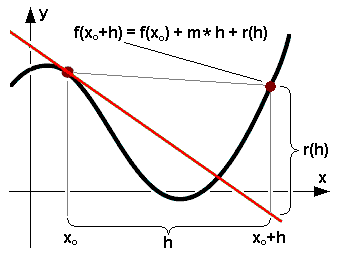
\includegraphics[width=0.4\textwidth]{pictures/diff-definition.png}\end{center} %70% der Textbreite%TODO: Bild selber machen
\end{*anmerkung}

\begin{*anmerkung}
	Neben der oben genannten Definition gibt es noch eine weitere Definition, die sich des Differentialquotienten bedient:
	\begin{align}
		f\text{ differentierbar in }x_0 \iff \lim\limits_{x\to x_0}\frac{f(x)-f(x_0)}{x-x_0}= \lim\limits_{h\to 0}\frac{f(x_0+h)-f(x_0)}{h}\text{ exisitiiert}\notag
	\end{align}
	Diese Definition lässt sich im Kontext komplexer oder mehrdimensionaler Funktionen nicht anwenden, zudem sind Beweise wegen des Quotienten leichter zu führen.
\end{*anmerkung}

\begin{*remark}
	Affin lineare Abbildung $\tilde{A}(x) := f(x_0) + f'(x_0)\cdot(x-x_0)$ approximiert die Funktion $f$ in der Nähe von $x_0$ und heißt \begriff{Linearisierung} von $f$ in $x_0$ (man nennt \propref{definition_ableitung} auch Approximation 1. Ordnung von $f$ in der Nähe von $x_0$).
\end{*remark}

\begin{proposition}
	\proplbl{definition_ableitung_proposition}
	Sei $f:D\subset K^n\to K^m$, $D$ offen. Dann: \\
	$f$ ist differenzierbar in $x_0\in D$ mit Ableitung $f'(x_0) \in L(K^n, K^m)$ \gls{gdw} eine der folgenden Bedingungen erfüllt ist:
	\begin{enumerate}[label={\alph*)},mode=unboxed]
		\item \label{satz_equivalenz_ableitungen_a} \itemEq{\proplbl{definition_ableitung_eins}f(x) &= f(x_0) + f'(x_0) \cdot (x-x_0) + r(x) \quad \forall x\in D}
		für ein $r: D\to K^m$ mit $\lim\limits_{\substack{x\to x_0 \\ x\neq x_0}} \frac{r(x)}{\vert x - x_0 \vert} = 0$
		\item \proplbl{satz_equivalenz_ableitungen_b} \itemEq{f(x) =f(x_0) + f'(x_0) \cdot (x-x_0) + R(x) (x-x_0)\quad\forall x\in D\proplbl{definition_ableitung_zwei}}
		für ein $R:D \to L(K^n, K^m)$ ($\cong K^{m\times n}$) mit $\lim\limits_{x\to x_0} R(x) = 0$ (d.h. Matrizen $R(x) \xrightarrow{x\to x_0}$ Nullmatrix in $K^{m\times n}$)
		\item \label{satz_equivalenz_ableitungen_c} \itemEq{\proplbl{definition_ableitung_drei}f(x) = f(x_0) + Q(x) (x - x_0) \quad \forall x\in D} für ein $Q:D\to L(K^n, K^m)$ ($\cong K^{m\times n}$) mit $\lim\limits_{x\to x_0} Q(x) = f'(x_0)$ (d.h. Matrizen $Q(x) \xrightarrow{x\to x_0}$ Matrix $f'(x_0)$ in $K^{m\times n}$)
	\end{enumerate}
\end{proposition}

\begin{*remark}
	Es gilt:
	\begin{align*}
	\text{\propref{definition_ableitung_eins}}\; \Leftrightarrow\; \lim\limits_{\substack{x\to x_0 \\ x\neq x_0}} \frac{f(x) - f(x_0) - f'(x_0) (x - x_0)}{\vert x - x_0 \vert} = 0
	\end{align*}
\end{*remark}

\begin{proof}
	\NoEndMark
	Aussage \ref{satz_equivalenz_ableitungen_a} ist leicht zu zeigen, anschließend erfolgt per Ringschluss die Äquivalenz der anderen Definitionen.
	\begin{enumerate}[label={zu \alph*)},leftmargin=\widthof{\ zu a)\ }]
		\item Offensichtlich ist $r(x) = o(\vert x - x_0 \vert ),$ $x\to x_0$ \\
		$\Rightarrow\;$ \ref{satz_equivalenz_ableitungen_a} $\Leftrightarrow$ $f$ ist differenzierbar in $x_0$ mit Ableitung $f'(x_0)$
	\end{enumerate}
	Ringschluss:
	\begin{itemize}[leftmargin=\widthof{\ a) $\rightarrow$ b):\ },topsep=-5pt]
		\item[a) $\Rightarrow$ b):] Sei $R: D\to K^{m\times n}$ gegeben durch \marginnote{$\otimes$: Tensorprodukt (siehe \cpageref{definition_tensorprodukt})}\begin{align*}
			R(x) &= \begin{cases}
				0, & x = x_0 \\
				\frac{r(x)}{\vert x - x_0\vert} \otimes (x - x_0)^T, & x\neq x_0
			\end{cases}\\
			\Rightarrow \;R(x) (x - x_0) &= \left( \frac{r(x)}{\vert x - x_0\vert^2} \otimes (x - x_0)^T \right) \cdot (x - x_0)\\
			 &= \frac{r(x)}{\vert x - x_0\vert ^2} \cdot \langle x - x_0 , x - x_0 \rangle = r(x) \quad \forall x\neq x_0
		\end{align*}
		Wegen $0 = r(x_0) = R(x_0)\cdot (x - x_0)$ folgt \begin{align*}
			\lim\limits_{x\to x_0} \vert R(x) \vert = \lim\limits_{\substack{x\to x_0 \\ x\neq x_0}} \frac{\vert r(x) \otimes (x - x_0)^T\vert }{\vert x - x_0 \vert^2} = \lim\limits_{\substack{x\to x_0 \\ x\neq x_0}} \frac{\vert r(x)\vert}{\vert x - x_0\vert} = 0
			\end{align*}
			
		\item[b) $\Rightarrow$ c):] Setzte $Q(x) := f'(x_0) + R(x) \; \forall x\in D$ $\Rightarrow$ \propref{definition_ableitung_drei}. Wegen $\lim\limits_{x\to x_0} Q(x) = f'(x_0)$ folgt \ref{satz_equivalenz_ableitungen_c}.
			
		\item[c) $\Rightarrow$ a):] Setzte $r(x) := (Q(x) - f'(x))\cdot (x - x_0) \;\forall x\in D$ $\Rightarrow$ \propref{definition_ableitung_eins}. Wegen $\vert r(x) \vert \le \vert Q(x) - f'(x_0) \vert \cdot \vert x - x_0 \vert $ folgt \zeroAmsmathAlignVSpaces \begin{align*}
			\lim\limits_{\substack{x\to x_0 \\ x\neq x_0}} \frac{\vert r(x) \vert}{\vert x - x_0 \vert} =  \lim\limits_{\substack{x\to x_0 \\ x\neq x_0}} \vert Q(x) - f'(x_0) \vert = 0
		\end{align*}
		\hfill$\square$
	\end{itemize}
\end{proof}

\begin{proposition}
	\proplbl{diffbar_impl_stetig}
	Sei $f:D\subset K^n \to K^m$, $D$ offen, differenzierbar in $x_0\in D$. Dann:
	\begin{enumerate}[label={\arabic*)}]
		\item $f$ ist stetig in $x_0$
		\item Die Ableitung $f'(x_0)$ ist eindeutig bestimmt.
	\end{enumerate}
\end{proposition}

\begin{proof}
	\begin{enumerate}
		\item Sei $A,\tilde{A}\in L(K^n,K^m)$ Ableitungen von $f$ in $x_0$, betrachte $x=x_0+ty$, wobei $y\in K^n$ mit $\vert y\vert =1$ fest, $t\in\real_{>0}$ (offenbar $\vert x-x_0\vert=t$) \\
		$\Rightarrow (A-\tilde{A})(ty)=o(\vert ty\vert)\Rightarrow (A-\tilde{A})(y)=\frac{o(t)}{t}\to 0$ \\
		$\Rightarrow (A-\tilde{A})(y)=0\Rightarrow A-\tilde{A}=0\Rightarrow A=\tilde{A}\beha$
		\item $\lim f(x)=1=\lim\big(f(x_0)+f'(x_0)(x-x_0)+o(\vert x-x_0\vert)\big)=f(x_0)\beha$
	\end{enumerate}
\end{proof}

\subsection{Spezialfälle für \texorpdfstring{$K=\mathbb{R}$}{K=R}}
\begin{enumerate}[label={\arabic*)},leftmargin=\widthof{1)\ },topsep=-5pt]
	\item \proplbl{spezialfall_ableitung_m1_item} \uline{$m=1\negthickspace:\, f\negthickspace:\mathbb{R}^n\to \mathbb{R}$}\\[0.6ex]
	$f'(x_0)\in \mathbb{R}^{1\times n}$ ist Zeilenvektor, $f'(x_0)$ betrachtet als Vektor im $\mathbb{R}^n$ auch \begriff{Gradient} genannt.
	
	Offenbar gilt $f'(x_0)\cdot y = \langle f'(x_0), y\rangle\;\forall y\in\mathbb{R}^n$ (Matrizenmultiplikation = Skalarprodukt) \\
	$\Rightarrow$ \propref{definition_ableitung_zwei} hat die Form \begin{align}
		\proplbl{spezialfall_ableitung_m1}
		f(x) = \underbrace{f(x_0) + \langle f'(x_0), x - x_0\rangle}_{\mathclap{\text{affin lineare Funktion: }\tilde{A}: \mathbb{R}\to \mathbb{R} \,(\text{in }x)}} + o\big( \vert x - x_0\vert \big)
	\end{align}
	Graph von $f$ ist Fläche im $\mathbb{R}^{n\times 1}$, genannt \begriff{Tangentialebene} vom Graphen von $f$ in $\big(x_0, f(x_0)\big)$.
	
	\item \proplbl{spezialfall_ableitung_n1} \uline{$n=1\negthickspace: f\negthickspace: D\subset \mathbb{R}\to \mathbb{R}^n$}\\[0.6ex]
	$f$ (bzw.  Bild $f[D]$) ist Kurve im $\mathbb{R}^n$ ($\cong \mathbb{R}^{m\times 1}$). \propref{definition_ableitung_zwei} kann man schreiben als \begin{align*}
		f(x_0 + t) = \underbrace{f(x_0) + t\cdot f'(x_0)}_{\mathclap{\text{Affin lineare Abb. }\tilde{A}:\mathbb{R}\to \mathbb{R}^m \text{ (in $t$)}}} + o(t), t\to 0, t\in\mathbb{R}
	\end{align*}
	\zeroAmsmathAlignVSpaces
	\begin{alignat}{2}
		\notag &\Leftrightarrow\quad& \underbrace{\frac{f(x_0 + t) - f(x_0)}{t}}_{\mathclap{\text{\begriff{Differenzenquotient} von $f$ in $x_0$}}} &= f'(x_0) + o(1), t\to 0 \\
		\proplbl{differentialquotient} &\Leftrightarrow& \underbrace{\lim\limits_{t\to 0} \frac{f(x_0 + t) - f(x_0)}{t}}_{\mathclap{\text{Differentialquotient}}} &= f(x_0)
	\end{alignat}
	
	\emph{beachte:} \begin{itemize}
		\item $f$  \gls{diffbar} in $x_0$ $\Leftrightarrow$ Differentialquotient existiert in $x_0$
		\item \propref{differentialquotient} nicht erklärt im Fall von $n>1$
	\end{itemize}

	\begin{interpretation}[ für $m > 1$]
		$f'(x_0)$ heißt \begriff{Tangentenvektor} an die Kurve in $f(x_0)$. Falls $f$ nicht  \gls{diffbar} in $x_0$ bzw. $x_0$ Randpunkt in $D$ und ist $f(x_0)$ definiert, so betrachtet man in \propref{differentialquotient} auch einseitige Grenzwerte (vgl. \propref{einseitige_grenzwerte}).
		
		$\lim\limits_{t\downarrow 0} \frac{f(x_0 + t) - f(x_0)}{t} = f_r'(x_0)$ heißt \begriff[Ableitung!]{rechtsseitige} \uline{Ableitung} von $f$ in $x_0$ (falls existent), analog ist $\lim\limits_{t\uparrow 0}$ die \begriff[Ableitung!]{linksseitige} \uline{Ableitung} $f_l'(x_0)$.
	\end{interpretation}

	\item \uline{$n=m=1\negthickspace:\;f\negthickspace: D\subset \mathbb{R}\to \mathbb{R}$} (vgl. Schule)\\[0.6ex]
	$f'(x_0)\in \mathbb{R}$ ist Zahl und \propref{differentialquotient} gilt (da Spezialfall von \propref{spezialfall_ableitung_n1}).
	
	\emph{Beobachtung:} \propref{spezialfall_ableitung_n1} gilt allgemein für $n=1$, nicht für $n>1$!
\end{enumerate}
\vspace*{1.5
	em}

\begin{conclusion}
	Sei $f:D\subset K\to K^n$, $D$ offen. Dann:
	\begin{align}
		\notag& \text{$f$ ist differenzierbar in $x_0\in D$ mit Ableitung $f'(x_0)\in L(K, K^m)$} \\
		\Leftrightarrow\quad
		& \proplbl{differentialquotient_prop} \exists f'(x_0) \in L(K, K^m): \lim\limits_{y\to 0} \frac{f(x_0 + y) - f(x_0)}{y} = f'(x_0) \\
		\notag 
		& \text{alternativ: } \lim\limits_{x\to x_0} \frac{f(x) - f(x_0)}{x - x_0} = f'(x_0)
	\end{align}
\end{conclusion}

\subsection{Einfache Beispiele für Ableitungen}
\begin{example}[affin lineare Funktionen]
	\proplbl{ableitung_linear}
	Sei $f:K^n\to K^m$ affin linear, d.h. \begin{align*}
		f(x) = A\cdot x + a\quad \forall x\in K^n, \text{ mit } A\in L(K^n, K^m), \, a\in K^m \text{ fest}
	\end{align*}
	Dann gilt für beliebiges $x_0\in K^n$:
	\zeroAmsmathAlignVSpaces**
	\begin{align*}
		f(x) &= A\cdot x_0 + a + A(x - x_0) \\
		&=f(x_0) + A(x - x_0)
	\end{align*}
	\zeroAmsmathAlignVSpaces
	\begin{align*}
		\xRightarrow{(\ref{definition_ableitung})}\;\; \text{$f$ ist  \gls{diffbar} in $x_0$ mit } f'(x_0) = A
	\end{align*}
	Insbesondere gilt für konstante Funktionen $f'(x_0) = 0$
	\begin{center}\begin{tikzpicture}
		\begin{axis}[
		xmin=-5, xmax=5, xlabel=$x$,
		ymin=-5, ymax=5, ylabel=$y$,
		samples=400,
		axis y line=middle,
		axis x line=middle,
		]
		\addplot+[mark=none] {2*x};
		\addlegendentry{$2x$}
		\addplot+[mark=none, dashed] {2};
		\addlegendentry{$2$}
		\end{axis}
		\end{tikzpicture}\end{center}
\end{example}

\begin{example}[quadratische Funktion]
	\proplbl{ableitung_beispiel_euklidische_norm}
	Sei $f:\real^n\to \real$ mit $f(x)=\vert x\vert^2$ \\
	für beliebiges $x_0$ gilt:
	\begin{align}
		\vert x-x_0\vert^2 &= \langle x-x_0,x-x_0\rangle \notag \\
		&= \vert x\vert^2 - \vert x_0\vert^2 - 2\langle x_0,x-x_0\rangle \notag
	\end{align}
	$\Rightarrow f(x) = f(x_0) + 2\langle \underbrace{2x_0}_{\text{Ableitung}},x-x_0\rangle + \underbrace{\vert x-x_0\vert^2}_{o(\vert x-x_0\vert)}$ \\
	$\Rightarrow f$ ist differenzierbar in $x_0$ mit $f'(x_0)=2x_0$, offenbar ist $f'$ stetig, also $f\in C^1(\real^n)$
 	\begin{center}\begin{tikzpicture}
 		\begin{axis}[
 		xmin=-5, xmax=5, xlabel=$x$,
 		ymin=-5, ymax=5, ylabel=$y$,
 		samples=400,
 		axis y line=middle,
 		axis x line=middle,
 		]
 		\addplot+[mark=none] {abs(x)^2};
 		\addlegendentry{$\vert x\vert^2$}
 		\addplot+[mark=none, dashed] {2*x};
 		\addlegendentry{$2x$}
 		\end{axis}
 		\end{tikzpicture}\end{center}
\end{example}

\begin{example}[Funktionen mit höherem Exponent]
	Sei $f:K\to K$, $f(x) = x^k$, $k\in\mathbb{N}$.
	\begin{itemize}[leftmargin=\widthof{$\,k=0$:\ }]
		\item[$k=0$:] $f(x) = 1\;\forall x$ $\Rightarrow$ $f'(x_0) = 0\;\forall x_0\in\mathbb{C}$ (vgl. \propref{ableitung_linear})
		\item[$k\ge 1$:] Es gilt \\
		\renewcommand{\arraystretch}{1.2}
		\begin{tabularx}{\linewidth}{r@{\ \ }r@{$\,$}X}
			& $(x_0 + y)^k$ & $\displaystyle = \sum_{j=0}^{k}\binom{k}{j} x_0^{k-j}\cdot y^j = x_0^k + k\cdot x_0^{k-1}\cdot y + o(y),\;y\to 0$ \\
			$\Rightarrow$ & $f(x_0 + y)$ & $= f(x_0) + k\cdot x_0^{k-1}\cdot y + o(y), y\to 0$ \\
			$\xRightarrow{(\ref{definition_ableitung})}$ & $f'(x_0)$ & $= k\cdot x_0^{k-1}$
		\end{tabularx}
	\end{itemize}
	\emph{beachte:} gilt in $\mathbb{C}$ und $\mathbb{R}$.
	\begin{center}\begin{tikzpicture}
		\begin{axis}[
		xmin=-5, xmax=5, xlabel=$x$,
		ymin=-5, ymax=5, ylabel=$y$,
		samples=400,
		axis y line=middle,
		axis x line=middle,
		]
		\addplot+[mark=none] {x^3};
		\addlegendentry{$x^3$}
		\addplot+[mark=none, dashed] {3*x^2};
		\addlegendentry{$3x^2$}
		\end{axis}
		\end{tikzpicture}\end{center}
\end{example}

\begin{example}[Exponentialfunktion]
	$f:K\to K$ mit $f(x)=e^x$ \\
	mit Differentialquotient $\Rightarrow$ $f$ ist differenzierbar mit $f'(x_0)=e^{x_0}\Rightarrow f\in C^1(K)$
	\begin{center}\begin{tikzpicture}
		\begin{axis}[
		xmin=-5, xmax=5, xlabel=$x$,
		ymin=-5, ymax=5, ylabel=$y$,
		samples=400,
		axis y line=middle,
		axis x line=middle,
		]
		\addplot+[mark=none] {e^x};
		\addlegendentry{$e^x$}
		\addplot+[mark=none, dashed] {e^x};
		\addlegendentry{$e^x$}
		\end{axis}
		\end{tikzpicture}\end{center}
\end{example}

\begin{example}[Betragsfunktion]
	\proplbl{ableitung_beispiel_betrag}
	$f:\real^n\to \real$ mit $f(x)=\vert x\vert$ \\
	$f$ ist nicht differenzierbar in $x_0=0$, denn angenommen, $f'(x_0)\in\real^n$ existiert und fixiere $y\in\real^n$, $\vert y\vert=1$ \\
	$\Rightarrow \vert ty\vert=0+\langle f'(0),ty\rangle + o(\vert t\vert)$, $t\to 0$ \\
	$\Rightarrow t\neq 0\Rightarrow \frac{\vert t\vert}{t}=\langle f'(0),y\rangle+\frac{o(t)}{t}\Rightarrow\pm 1 =$ feste Zahl in $\real_+\to 0\Rightarrow\lightning\beha$
	
	\emph{Folglich:} $f$ stetig in $x_0\not\Rightarrow f$ differenzierbar in $x_0$, das heißt Umkehrung von \propref{diffbar_impl_stetig} gilt nicht!
	
	\begin{hint}
		Es gibt stetige Funktion $f:\mathbb{R}\to \mathbb{R}$, die in keinem Punkt $x$ \gls{diffbar} ist (siehe Hildebrand, Analysis 1 S. 192 oder Königsberger Analysis 1, Kap. 9.11)
	\end{hint}

	\begin{center}\begin{tikzpicture}
		\begin{axis}[
		xmin=-5, xmax=5, xlabel=$x$,
		ymin=-5, ymax=5, ylabel=$y$,
		samples=400,
		axis y line=middle,
		axis x line=middle,
		]
		\addplot+[mark=none] {abs(x)};
		\addlegendentry{$\vert x \vert$}
		\end{axis}
	\end{tikzpicture}\end{center}
\end{example}

\begin{proposition}[Rechenregeln]
	\proplbl{ableitung_rechenregeln}
	Sei $D\in K^n$ offen, $f,g: D\to K^m$, $\lambda: D\to K$  \gls{diffbar} in $x_0\in D$ \\
	$\Rightarrow$ $(f\pm g): D\to K^m, (\lambda\cdot f):D\to K^m, (f\cdot g):D\to K$ sind  \gls{diffbar} in $x_0\in D$ und $\frac{1}{\lambda}:D\to K$ ist  \gls{diffbar} in $x_0$, falls $\lambda(x_0)\neq 0$
	mit
	\begin{enumerate}[label={\alph*)}]
		\item $(f\pm g)'(x_0) = f'(x_0) \pm g'(x_0)\in K^{m\times 1}$
		\item $(\lambda\cdot f)'(x_0) = \lambda (x_0)\cdot f'(x_0) + f(x_0)\cdot \lambda'(x_0)\in K^{m\times n}$
		\item $(f\cdot g)' (x_0) = \transpose{f(x_0)}\cdot g'(x_0) + \transpose{g(x_0)}\cdot f'(x_0)\in K^{m\times n}$
		\item $\left( \frac{\mu}{\lambda}\right)'(x_0) = \frac{\mu'(x_0)\cdot\lambda(x_0)-\mu(x_0)\cdot \lambda'(x_0)}{(\lambda(x_0))^2}$
	\end{enumerate}
\end{proposition}
\begin{proof}
	\begin{itemize}
		\item $f(x_0)\pm g(x_0)+(f'(x_0))(x-x_0)\pm (g'(x_0))(x-x_0)+o(\vert x-x_0\vert) =f(x_0)\pm g(x_0)+\big(f'(x_0)\pm g'(x_0)\big)(x-x_0)+o(\vert x-x_0\vert)\beha$
		\item $\lambda(x)f(x)=\big(\lambda(x_0)+\lambda'(x_0)(x-x_0)+o(\vert x-x_0\vert)\big)\cdot\big(f(x_0)+f'(x_0)(x-x_0)+o(\vert x-x_=\vert)\big) = \lambda(x_0)f(x_0) - \big(\lambda'(x_0)f(x_0)+\lambda(x_0)f'(x_0)\big)(x-x_0)+o(\vert x-x_0\vert)\beha$
		\item analog
		\item zeige $\left(\frac{1}{\lambda}\right)'(x_0)=-\frac{\lambda'(x_0)}{\lambda(x_0)^2}$, Rest folgt mit $f=\mu$ \\
		$\frac{1}{\lambda(x)}-\frac{1}{\lambda(x_0)}=\frac{\lambda(x_0)-\lambda(x)}{\lambda(x)\lambda(x_0)} = ... = \left(\frac{-\lambda'(x_0)}{\lambda(x_0)^2}\right)(x-x_0)+o(\vert x-x_0\vert)\beha$
	\end{itemize}
\end{proof}

\begin{example}
	Sei $f:D\in K^n\to K^m$, $c\in K$, $f$  \gls{diffbar} in $x_0\in D$\\
	$\xRightarrow{\ref{ableitung_rechenregeln}\ b)} (c\cdot f) = c\cdot f'(x_0)$ (da $c$ konst. Funktion $D\to K$)
\end{example}

\begin{example}[Polynom]
	Sei $f:K\to K$, Polynom $f(x) = \sum\limits_{l=0}^{k}a_l x^l$ \\
	$\Rightarrow$ $f$  \gls{diffbar} $\forall x_0\in K$ mit $f'(x_0) = \sum\limits_{l=1}^k l a_l x_0^{l-1}$
\end{example}

\begin{example}
	Sei $f=\frac{f_1}{f_2}$ rationale Funktion auf $\mathbb{R}$ (d.h. $f_1, f_2:K\to K$ Polynom) \\
	$\Rightarrow$ $f$ ist  \gls{diffbar} auf $K\setminus \{ \text{Nullstellen von }f_2 \}$
\end{example}

\begin{example}[Sinus und Cosinus]
	$\sin, \cos: K\to K$ ($\mathbb{R}$ bzw. $\mathbb{C}$) $\forall x_0\in K$.
	
	Denn:{\zeroAmsmathAlignVSpaces
	\begin{align*}
		 \frac{\sin y}{y} = \frac{e^{iy} - e^{-iy}}{2iy} = \frac{1}{2}\cdot \left( \frac{e^{iy} - 1}{iy} + \frac{e^{-iy} - 1}{-iy} \right) \xrightarrow[\text{vgl. \eqref{exp_limit_1}}]{y\to 0} 1,
	\end{align*}}
	folglich {\zeroAmsmathAlignVSpaces*
	\begin{align*}
		\lim\limits_{y\to 0} \frac{\sin(x_0 + y) - \sin(x_0)}{y} &\overset{\star}{=} \lim\limits_{y\to 0} \frac{2}{y} \cos\left( x_0 + \frac{y}{2}\right) \cdot \sin \left( \frac{y}{2}\right) \marginnote{$\star$: Additionstheoreme} \\
		&= \lim\limits_{y\to 0} \frac{2}{y}\cdot\sin\left(\frac{y}{2}\right)\cdot\cos\left(x_0 + \frac{y}{2}\right)\\
		&= \cos x_0 \quad\forall x_0\in K
		\end{align*}}
		
	Analog für den Kosinus.
	
	\begin{center}\begin{tikzpicture}
		\begin{axis}[
		xmin=-5, xmax=5, xlabel=$x$,
		ymin=-5, ymax=5, ylabel=$y$,
		samples=400,
		axis y line=middle,
		axis x line=middle,
		]
		\addplot+[mark=none] {sin(deg(x))};
		\addlegendentry{$\sin(x)$}
		\addplot+[mark=none, dashed] {cos(deg(x))};
		\addlegendentry{$\cos(x)$}
		\end{axis}
		\end{tikzpicture}
		\begin{tikzpicture}
		\begin{axis}[
		xmin=-5, xmax=5, xlabel=$x$,
		ymin=-5, ymax=5, ylabel=$y$,
		samples=400,
		axis y line=middle,
		axis x line=middle,
		]
		\addplot+[mark=none] {cos(deg(x))};
		\addlegendentry{$\cos(x)$}
		\addplot+[mark=none, dashed] {- sin(deg(x))};
		\addlegendentry{$-\sin(x)$}
		\end{axis}
		\end{tikzpicture}\end{center}
\end{example}

\subsection{Rechenregeln}
\begin{*definition}
	Sei $f:D\subset K^n \to K^m$, $D$ offen.
	
	Falls $f$  \gls{diffbar} in allen $x_0\in D$, dann heißt $f$ \begriff{differenzierbar} auf $D$ und Funktion $f':D\to L(K^n, K^m)$ heißt \begriff{Ableitung} von $f$.
	
	Ist zusätzlich Funktion $f': D\to L(K^n, K^m)$ stetig, dann heißt Funktion $f$ \begriff{stetig differenzierbar} (auf $D$) bzw. \mathsymbol{C1}{$C^1$}\emph{-Funktion} (auf $D$).
	
	$C^1(D, K^m):= \left\lbrace f: D\to K^m \mid f \text{ stetig  \gls{diffbar} auf } D \right\rbrace$
\end{*definition}

\begin{example}
	\begin{enumerate}[label={\alph*)}]
		\item $f(x) = x^k\;\forall x\in\mathbb{R},\, k\in\mathbb{N}_{\ge 0}$ \\
		$\Rightarrow$ $f'(x) = k\cdot x^{k-1}\;\forall x\in \mathbb{R}$ \\
		$\Rightarrow$ offenbar stetige Funktion \\ $\Rightarrow$ $f\in C^1(\mathbb{R}, \mathbb{R})$
		
		\item $f(x) = e^x\;\forall x\in\mathbb{C}$ \\
		$\Rightarrow f'(x) = e^x \;\forall x\in\mathbb{C}$ stetig \\
		$\Rightarrow$ $f\in C^1(\mathbb{C},\mathbb{C})$
		
		\item $f(x) = \vert x \vert^2\;\forall x\in\mathbb{R}^n$ \\
		$\Rightarrow$ $f(x) = 2x\;\forall x\in\mathbb{R}^n$, offenbar stetig \\
		$\Rightarrow$ $f\in C^1(\mathbb{R}^n, \mathbb{R})$
	\end{enumerate}
\end{example}

\begin{example}
	\proplbl{ableitung_beipsiel_unstetige_ableitung}
	Sei $f:\mathbb{R}\to \mathbb{R}$ mit $f(0) = 0$, $f(x)=x^2\cdot \sin\left(\frac{1}{x}\right)$ $\forall x\neq 0$.
	
	\begin{center}\begin{tikzpicture}
		\begin{axis}[
		xmin=-5, xmax=5, xlabel=$x$,
		ymin=-5, ymax=5, ylabel=$y$,
		samples=400,
		axis y line=middle,
		axis x line=middle,
		]
		\addplot+[mark=none] {x^2*sin(deg(1/x))};
		\addlegendentry{$x^2\cdot \sin(\frac{1}{x})$}
		\end{axis}
		\end{tikzpicture}\end{center}
	
	Wegen \begin{align*}
		\frac{\vert x^2 \cdot \sin \frac{1}{x}\vert}{\vert x \vert} \le \vert x \vert \xrightarrow{x\neq 0} 0
	\end{align*}
	folgt{ \zeroAmsmathAlignVSpaces \begin{align*}
		& f(x) = o(\vert x \vert), x\to 0 \\
		\Rightarrow\;& f(x) = f(0) + 0\cdot (x - 0) + o(\vert x - 0\vert), x\to 0 \\
		\Rightarrow\;& f \text{  \gls{diffbar} in $x=0$ mit $f'(0) = 0$}
	\end{align*}}
	
	Rechenregeln liefern $x\neq 0$: \begin{align*}
		f'(x) = 2x\cdot\sin\frac{1}{x}- \cos\frac{1}{x} \quad\forall x\neq 0
	\end{align*}
	
	Für $x_k := \frac{1}{k\pi}$ gilt: \begin{align*}
		& \lim\limits_{k\to\infty} 2 x_k \cdot \sin \frac{1}{x_k} = 0,\; \lim\limits_{k\to\infty} \cos \frac{1}{x_k} = \pm 1 \\
		\Rightarrow\;& \lim\limits_{x\to 0} f'(x) \text{ existiert nicht} \\
		\Rightarrow\;& f\notin C^1(\mathbb{R}, \mathbb{R}),
	\end{align*}
	d.h. Ableitung einer stetigen Funktion muss \emph{nicht} stetig sein.
\end{example}

\begin{boldenvironment}[Man beobachtet]
	\hspace{0pt}
\begin{itemize}[topsep=-2pt]
	\item \propref{definition_ableitung} bzw. \propref{definition_ableitung_zwei_stern} sind häufig ungeeignet zum Bestimmen von $f'(x_0)$
	\item \propref{differentialquotient_prop} ist durchaus nützlich für konkrete Fälle im Fall $n=1$
	
	\emph{$\rightarrow$ Strategie:} Zurückführung auf einfachere Fälle durch Rechenregeln und Reduktion
\end{itemize}
\end{boldenvironment}



\begin{conclusion}
	\proplbl{ableitung_quotientenregel}
	Seien $\lambda$, $\mu:D\to K$  \gls{diffbar} in $x_0$, $D$ offen und $\lambda(x_0)\neq 0$ \\
	$\Rightarrow$ $\left( \frac{\mu}{\lambda} \right): D\to K$  \gls{diffbar} in $x_0$ mit \begin{align*}
		\left( \frac{\mu}{\lambda} \right)' (x_0) = \frac{\lambda(x_0)\cdot \mu'(x_0) - \mu(x_0) \cdot \lambda'(x_0)}{\lambda(x_0)^2}\in K^{1\times n}
	\end{align*}
\end{conclusion}

\begin{proof}[\propref{ableitung_quotientenregel}]
	Setzte in \propref{ableitung_rechenregeln} $f=\mu$ (d.h. $m=1$) und betr. Produkt $\frac{1}{\lambda}\cdot \mu$.
\end{proof}

\begin{proposition}[Kettenregel]
	\proplbl{ableitung_kettenregel}
	Sei $f:D\subset K^n\to K^m$, $g:\tilde{D}\subset K^m\to K^l$, $D$,$\tilde{D}$ offen, $f$  \gls{diffbar} in $x_0\in D$, $g$  \gls{diffbar} in $f(x_0)\in\tilde{D}$ \\
	$\Rightarrow$ $g\circ f: D\to K^l$  \gls{diffbar} in $x_0$ mit $(g\circ f)' = g'(f(x))\cdot f'(x)$ ($\in K^{l\times n}$)
\end{proposition}
\begin{proof}
	\begin{align}
		(g\circ f)(x)  = g(f(x)) &= g(f(x_0)) + g'(f(x_0))(f(x)-f(x_0)) + o(\vert f(x)-f(x_0)\vert) \notag \\
		&= (g\circ f)(x_0) + g'(f(x_0))\cdot f(x_0)(x-x_0) + o(\vert x-x_0\vert)
	\end{align}
	$\Rightarrow$ Behauptung
\end{proof}

\begin{example}[$x$ im Exponenten]
	\proplbl{ableitung_beispiel_exponentialfunktion}
	$f:\mathbb{R}\to \mathbb{R}$, $f(x) = a^x$ ($a\in\mathbb{R}_{\ge 0}$, $a\neq 1$).
	Offenbar $a^x = \left(e^{\ln a}\right)^x = e^{x\cdot \ln a}$\\
	$\Rightarrow$ $f(x) = g(h(x))$ mit $g(y) = e^y$, $h(x) = x\cdot \ln a$
	$\Rightarrow g'(y)=e^y$, $h'(x)=\ln a\Rightarrow f'(x)=e^{x\cdot \ln a}\cdot \ln a=a^x\cdot\ln a$
	\begin{center}\begin{tikzpicture}
		\begin{axis}[
		xmin=-5, xmax=5, xlabel=$x$,
		ymin=-5, ymax=5, ylabel=$y$,
		samples=400,
		axis y line=middle,
		axis x line=middle,
		]
		\addplot+[mark=none] {2^x};
		\addlegendentry{$2^x$}
		\addplot+[mark=none, dashed] {2^x*ln(2)};
		\addlegendentry{$2^x\cdot \ln(2)$}
		\end{axis}
		\end{tikzpicture}\end{center}
\end{example}

\begin{example}[Logarithmus]
	\proplbl{ableitung_beispiel_logarithmus}
	$f:\real_{>0}\to \real$ mit $f(x)=\log_a x$, $a\in\real_{>0}$ und $a\neq 1$, $x_0\in \real_{>0}$ \\
	mit $y=\log_a x$, $y_0=\log_a x_0$ ist $x-x_0=a^y-a^{y_0}$ \\
	Differentialquotient $\Rightarrow f'(x)=\frac{1}{x\cdot\ln a}$, also $f\in C^1(\real_{>0})$
	
	Spezialfall: $(\ln(x))' = \frac{1}{x}$ $\forall x>0$
	\begin{center}\begin{tikzpicture}
		\begin{axis}[
		xmin=-5, xmax=5, xlabel=$x$,
		ymin=-5, ymax=5, ylabel=$y$,
		samples=400,
		axis y line=middle,
		axis x line=middle,
		]
		\addplot+[mark=none] {log2(x)};
		\addlegendentry{$\log_2(x)$}
		\addplot+[mark=none, dashed] {1/(x*ln(2))};
		\addlegendentry{$\frac{1}{x\cdot\ln(2)}$}
		\end{axis}
		\end{tikzpicture}\end{center}
\end{example}

\begin{example}
	Sei $f:\mathbb{R}_{>0}\to \mathbb{R}$, $f(x) = x^r$ ($r\in\mathbb{R}$)
	
	Wegen $x^r = e^{r\cdot \ln x}$ liefert Kettenregeln (analog zu \propref{ableitung_beispiel_exponentialfunktion}) \begin{align*}
	f'(x_0) = \frac{r\cdot e^{r\cdot \ln x_0}}{x_0} = \frac{r\cdot x_0^r}{x_0} = r\cdot x_0^{r - 1} \quad\forall x_0>0
	\end{align*}
	
	Spezialfall: $f(x) = \frac{1}{x^k}$ $\Rightarrow$ $f'(x) = - \frac{k}{x^{k+1}}$
	
	Zu \propref{ableitung_beipsiel_unstetige_ableitung}:\begin{align*}
	f'(x) = 2x\cdot \sin\frac{1}{x} + x^2\cdot \cos\frac{1}{x} \cdot \left( - \frac{1}{x^2}\right) = 2x\cdot \sin\frac{1}{x} - \cos\frac{1}{x}
	\end{align*}
\end{example}

\begin{example}[Tangens und Cotangens]
	\proplbl{ableitung_beispiel_tangens}
	$\tan: K\setminus \{ \frac{\pi}{2} + k\cdot \pi \mid k\in\mathbb{Z} \}\to K$, $\cot:K\setminus \{ k\cdot \pi \mid k\in\mathbb{Z} \} \to K$ \\[\dimexpr - \baselineskip / 2 \relax]
	\zeroAmsmathAlignVSpaces \begin{alignat*}{3}
	\xRightarrow{\text{Quotientenregel}}&\;\;& \tan'(x_0)&= \frac{\sin'(x_0)\cos (x_0) - \cos (x_0) \cdot \sin(x_0)}{\left( \cos(x_0)\right)^2} &&\\
	&& &= \frac{\cos^2(x_0) + \sin^2(x_0)}{\cos^2(x_0)} = \frac{1}{\cos^2(x_0)} && \forall x_0\in \text{ Definitionsbereich} \\
	&& \cot'(x_0) &= - \frac{1}{\sin^2(x_0)}&&\forall x_0\in\text{ Definitionsbereich}
	\end{alignat*}
	\begin{center}\begin{tikzpicture}
		\begin{axis}[
		xmin=-5, xmax=5, xlabel=$x$,
		ymin=-5, ymax=5, ylabel=$y$,
		samples=400,
		axis y line=middle,
		axis x line=middle,
		restrict y to domain=-5:5
		]
		\addplot+[mark=none] {tan(deg(x))};
		\addlegendentry{$\tan(x)$}
		\addplot+[mark=none, dashed] {1/(cos(deg(x)))^2};
		\addlegendentry{$\frac{1}{\cos^2(x)}$}
		\end{axis}
		\end{tikzpicture}
		\begin{tikzpicture}
		\begin{axis}[
		xmin=-5, xmax=5, xlabel=$x$,
		ymin=-5, ymax=5, ylabel=$y$,
		samples=400,
		axis y line=middle,
		axis x line=middle,
		restrict y to domain=-5:5
		]
		\addplot+[mark=none] {cot(deg(x))};
		\addlegendentry{$\cot(x)$}
		\addplot+[mark=none, dashed] {-1/(sin(deg(x))^2)};
		\addlegendentry{$-\frac{1}{\sin^2(x)}$}
		\end{axis}
		\end{tikzpicture}\end{center}
\end{example}





\begin{proposition}[Reduktion auf skalare Funktionen]
	\proplbl{ableitung_proposition_reduktion}
	Sei $f=(f_1, \dotsc, f_m): D\subset K^n\to K^m$, $D$ offen, $x_0\in D$. Dann gilt:\begin{center}
		$f$  \gls{diffbar} in $x_0$ $\Leftrightarrow$ alle $f_j$  \gls{diffbar} in $x_0$ $\forall j=1,\dotsc,m$
	\end{center}

	Im Fall der Differenzierbarkeit hat man: \begin{align}
		\proplbl{ableitung_jacobimatrix}
		f'(x_0) = \begin{pmatrix}
			f_1'(x_0) \\
			\vdots \\
			f_m'(x_0)
		\end{pmatrix} \in K^{m\times n}
	\end{align}
\end{proposition}
\smiley{} Wenn Sie das nächste mal aus der Disko kommen, zuviel getrunken haben und den Namen 
ihrer Freundin nicht mehr kennen, sollten sie sich daran aber noch erinnern: \smiley{} \\

\begin{remark}
	Mit \propref{ableitung_proposition_reduktion} kann man die Berechnungen der Ableitungen stets auf skalare Funktionen $f:D\subset K^n\to K$ zurückführen. Die Matrix in \propref{ableitung_jacobimatrix} besteht aus $m$ Zeilen $f_j'(x_0)\in K^{1\times m}$.
\end{remark}

\begin{example}
	Sei $f:\mathbb{R}\to \mathbb{R}^2$ mit \begin{align*}
		f(t) &= \begin{pmatrix}
			t\cdot \cos( 2\pi t) \\ t\cdot \sin(2\pi t)
		\end{pmatrix}, & f'(t) &= \begin{pmatrix}
			\cos(2\pi t) - t\cdot \sin(2\pi t)\cdot 2\pi \\ \sin(2\pi t)+ t\cdot\cos(2\pi t)\cdot 2\pi
		\end{pmatrix} \in \mathbb{R}^{2\times 1},
	\end{align*}
	und $f'(0) = \binom{1}{0}$, $f'(1) = \binom{1}{2\pi}$.
\end{example}

\begin{lemma}
	\proplbl{ableitung_spezialfall_reduktion_proposition}
	Sei $f=(f_1, f_2):D\subset K^n\to K^k\times K^l$, $D$ offen, $x_0\in D$.
	
	Funktion $f$ ist  \gls{diffbar} in $x_0$ genau dann, wenn $f_1:D\to K^k$ und $f_2 :D\to K^l$  \gls{diffbar} in $x_0$.
	
	Im Falle der Differenzierbarkeit gilt\begin{align}
		\proplbl{ableitung_spezialfall_reduktion}
		f'(x_0) = \begin{pmatrix}
			f_1'(x_0) \\ f_2'(x_0)
		\end{pmatrix} \in K^{(k+l)\times n}
	\end{align}
	
	\begin{hint}
		Da $K^k\times K^l$ mit $K^{k+l}$ identifiziert werden kann, kann man $f$ auch als Abbildung von $D$ nach $K^{k+l}$ ansehen. Dementsprechend kann die Matrix in \propref{ableitung_spezialfall_reduktion} der Form \begin{align*}
			\begin{pmatrix}
				(k\times n) \text{ Matrix} \\
				(l\times n) \text{ Matrix}
			\end{pmatrix}
		\end{align*}
		auch als $((k+l)\times n)$-Matrix aufgefasst werden.
	\end{hint}
\end{lemma}

\begin{proof}\hspace*{0pt}
	\NoEndMark
	\begin{itemize}[topsep=\dimexpr - \baselineskip / 3\relax]
		\item["`$\Rightarrow$"'] Man hat
		\zeroAmsmathAlignVSpaces[3pt][3pt]
		\begin{alignat}{2}
				\proplbl{ableitung_beweis_lemma_spezialfall_reduktion} && f(x) &= f(x_0) + f'(x_0)\cdot(x - x_0) + R(x)\cdot (x - x_0), \, \;R(x) \xrightarrow{x\to x_0}0
			\intertext{da $f'(x_0)$, $R(x)\in L(K^n, K^k\times K^l)$}
				\notag\Rightarrow&\;\;& f'(x_0) &= (A_1, A_2), \; R(x) = \big( R_1(x), R_2(x) \big))
			\intertext{mit $A_1, R_1(x)\in L(K^n, K^k)$, $A_2, R(x)\in L(K^n, K^l)$}
				\proplbl{ableitung_beweis_lemma_spezialfall_reduktion_einzelableitung} \xRightarrow{\eqref{ableitung_beweis_lemma_spezialfall_reduktion}}&& f_j(x)&= f_j(x_0) + A_j \cdot (x - x_0) + R_j(x) (x - x_0),\;R_j(x)\xrightarrow{x\to x_0}0 \\
				\notag\Rightarrow&& f_j & \text{ ist  \gls{diffbar} in $x_0$ mit $f_j'(x_0) = A_j$, $j=1,2$}
		\end{alignat}
		$\Rightarrow$ Behauptung
		\item["`$\Leftarrow$"'] (es gilt auch \eqref{ableitung_beweis_lemma_spezialfall_reduktion_einzelableitung} mit $A_j = f_j'(x_0)$)
		
		Setzte \begin{align*}
		 &A=\begin{pmatrix}
			f_1'(x) \\ f_2'(x)
		\end{pmatrix},\; R(x) = \begin{pmatrix}
			R_1(x) \\ R_2(x)
		\end{pmatrix} \\
		\xRightarrow{\eqref{ableitung_beweis_lemma_spezialfall_reduktion_einzelableitung}}\;& A, R(x)\in L(K^n, K^k\times K^l) \\
		\xRightarrow{\text{mit }A_j=f_j'(x_0)}\; & f(x)= f(x_0) + A(x - x_0) + R(x)(x - x_0), R(x)\xrightarrow{x\to x_0}0
		\end{align*}
		$\Rightarrow$ $f$  \gls{diffbar} in $x_0$ und \eqref{ableitung_spezialfall_reduktion} gilt.\hfill\csname\InTheoType Symbol\endcsname
	\end{itemize}
\end{proof}

\begin{proof}[\propref{ableitung_proposition_reduktion}]
	Mehrfache Anwendung von \propref{ableitung_spezialfall_reduktion_proposition} (z.B. mit $k=1, l = m - j$ für $j=1,\dotsc, m-1$)
\end{proof}
\section{Richtungsableitung und partielle Ableitung}\proplbl{richtungsableitung}  \setcounter{equation}{0}
Sei $f:D\subset K^n\to K^m$, $D$ offen, $x\in D$.

\begin{underlinedenvironment}[Ziel]
	Zurückführung der Berechnung der Ableitung $f(x)$ auf die Berechnung der Ableitung für Funktionen $\tilde{f}:\tilde{D}\subset K\to K$
	\begin{itemize}
		\item Reduktionssatz $\Rightarrow$ man kann sich bereits auf $m=1$ einschränken
		\item für Berechnung der Ableitung von $f$ ist neben den Rechen- und Kettenregeln auch der Differentialquotient verfügbar
	\end{itemize}
\end{underlinedenvironment}

\begin{underlinedenvironment}[Idee]
	Betrachte $f$ auf Geraden $t\to x + t\cdot z$ durch $x$ $\Rightarrow$ skalares Argument $t$, $t\in K$ $\Rightarrow$ Differentialquotient.
	
	Spezialfall: $z = e_j$ $\Rightarrow$ Partielle Ableitung
\end{underlinedenvironment}

\begin{*definition}
	Sei $f:D\subset K^n\to K^m$, $D$ offen, $x\in D$, $z\in K^n$.
	
	Falls $a\in L(K, K^m)$ ($\cong K^m$) existiert mit\begin{align}
		\proplbl{richtungsableitung_definition}
		f(x + t\cdot z) = f(x) + t\cdot a + o(t),\;t\to 0,\; t\in K,
	\end{align}
	dann heißt $f$ \gls{diffbar} in $x$ \begriff[differenzierbar!]{in Richtung $z$} und \mathsymbol{Dz}{$\mathrm{D}_z$}$f(x) := a$ heißt \begriff{Richtungsableitung} von $f$ in $x$ in Richtung $z$ (andere Bezeichnungen: $f(x; z)$, $\partial_z f(x)$, $\frac{\partial f}{\partial z}(x)$, $\partial f(x,z)$, $\dotsc$)
\end{*definition}
\begin{*remark}
	\begin{itemize}[topsep=\dimexpr -\baselineskip / 2\relax]
		\item Wegen $B_\epsilon(x)\subset D$ für ein $\epsilon > 0$ existiert $\tilde{\epsilon}$ mit $x + t\cdot z \in D$ $\forall t\in B_{\tilde{\epsilon}} (0) \subset K$
		\item $f'(x;0)$ existiert offenbar stehts für $z=0$ mit $f'(x;0) = 0$
	\end{itemize}
\end{*remark}

\begin{proposition}
	\proplbl{richtungsableitung_prop_equivalente_definition}
	Sei $f:D\subset K^n\to K^m$, $D$ offen, $x\in D$, $z\in K^n$. Dann:
	\begin{align}
		\notag &\text{$f$ \gls{diffbar} in $x$ in Richtung $z$ mit $\mathrm{D}_z f(x)\in L(K, K^m)$} \\
		\proplbl{richtungsableitung_definition_prop_eins}
		\Leftrightarrow\;\; & \text{für }\phi(t) = f(x + t\cdot z) \text{ existiert }\phi'(0) \text{ und } \mathrm{D}_z f(x) = \phi'(0) \\
		\proplbl{richtungsableitung_definitnion_prop_zwei}
		\Leftrightarrow\;\; & \lim\limits_{t\to 0} \frac{f(x + t\cdot z) - f(x)}{t} = a \;(\in L(K, K^m)) \text{ existiert und } \mathrm{D}_z f(x) = a
	\end{align}
\end{proposition}

\begin{example}
	Sei $f:\mathbb{R}^2\to\mathbb{R}$ mit $f(x) = x_1^2 + \vert x_2\vert$. Existiert eine Richtungsableitung in $x=(x_1, 0)$ in Richtung $z=(z_1, z_2)$?
	
	Sei $\phi(t) := f(x + t\cdot z) = (x_1 + t\cdot z_1)^2 + \vert t\cdot z_2\vert = \underbrace{x_1^2 + 2t\cdot x_1 z_1 + t^2 z_1^2}_{=\phi_1(t)} + \underbrace{\vert t \vert \cdot \vert z_2 \vert} _{=\phi_2(t)}$
	
	$\Rightarrow$ $\phi_1'(0) = 2\cdot x_1 z_1$ existiert $\forall x_1, z_1\in\mathbb{R}$ \\
	\phantom{$\Rightarrow$} $\phi_2'(0) = 0$ existiert \emph{nur} für $z_2 = 0$ (vgl. \propref{ableitung_beispiel_betrag}) \\
	$\Rightarrow$ $\phi_1'(0) = 2x_1z_1$ existiert \emph{nur} für $x_1$, $z_1\in\mathbb{R}$, $z_2 = 0$ \\
	$\xRightarrow{\eqref{richtungsableitung_definition_prop_eins}}$ Richtungsableitung von $f$ existiert für alle $ x = (x_1, 0)$ \emph{nur} in Richtung $z=(z_1, 0)$ mit $\mathrm{D}_z f(x) = 2x_1 z_1$
\end{example}

\begin{underlinedenvironment}[Frage]
	Existiert $\mathrm{D}_z f(x)$ $\forall z$, falls $f$ \gls{diffbar} in $x$?
\end{underlinedenvironment}

\begin{proposition}
	\proplbl{richtungsableitung_prop_existenz_prop}
	Sei $f:D\subset K^n\to K^m$, $D$ offen, $f$ \gls{diffbar} in $x\in D$.\\
	$\Rightarrow$ Richtungsableitung $\mathrm{D}_z f(x)$ existiert $\forall z\in K^n$ und \begin{align}
		\proplbl{richtungsableitung_prop_existenz}
		\mathrm{D}_z f(x) = f'(x) \cdot z \;(\in K^{m\times 1})
	\end{align}
	\emph{Hinweis:} Richtungsableitung ist linear in $z$!
\end{proposition}

\begin{proof}
	\NoEndMark
	$f$ \gls{diffbar} in $x$ \\
	\begin{tabularx}{\linewidth}{r@{\ \ }X}
		$\Rightarrow$ &$f(y) = f(x) + f'(x) (y - x) + o(\vert y - x\vert)$, $y\to x$ \\
		$\xRightarrow{y=x+t\cdot z}$& $f(x + tz) = f(x) + t\cdot f'(x)\cdot z + o(t)$, $t\to 0$ \\
		$\xRightarrow{\eqref{richtungsableitung_definition}}$&  Behauptung\hfill\csname\InTheoType Symbol\endcsname
	\end{tabularx}
\end{proof}

\begin{example}
	\proplbl{richtungsableitung_example_euklidische_norm}
	Betrachte $f:\mathbb{R}^n\to \mathbb{R}$ mit $f(x) = \vert x \vert ^2$ $\forall x$
	\begin{enumerate}[label={\alph*)}]
		\item Es gilt \zeroAmsmathAlignVSpaces \begin{alignat*}{2}
		 && \phi(t) &= \vert x + tz\vert ^2 = \sum_{i=1}^{n} (x_i + t z_i)^2 = \sum_{i=1}^n x_i^2 + 2t x_i z_i + t^2 z_i^2 \\
		 \Rightarrow && \phi'(t) &= \sum_{i=1}^n 2x_i z_i + 2t z_i^2 \\
		\xRightarrow{\eqref{richtungsableitung_definition_prop_eins}} &\;\;& \phi'(0) &= 2\sum_{i=1}^n x_i z_i = 2 \langle x,z\rangle = \mathrm{D}_z f(x)\quad\forall x, z\in\mathbb{R}^n
		\end{alignat*}
		\item \propref{ableitung_beispiel_euklidische_norm} liefert $f'(x) = 2x$ $\forall x\in\mathbb{R}^n$ \\
		$\xRightarrow{\eqref{richtungsableitung_prop_existenz}} $ $\mathrm{D}_z f(x) = 2x\cdot z = 2 \langle x,z\rangle$ $\forall x,z\in\mathbb{R}^n$
	\end{enumerate}
	folglich gilt: $\vert z \vert = 1$ und $x\in\mathbb{R}^n$ fest \begin{itemize}
		\item $\mathrm{D}_z f(x) = 0$ $\Leftrightarrow$ $x\perp z$
		\item $\mathrm{D}_z f(x) = \,$maximal ($x$ fest) $\Leftrightarrow$ $z = \frac{x}{\vert x \vert}$
	\end{itemize}
\end{example}

\subsection{Anwendung: Eigenschaften des Gradienten}
\begin{*definition}
	Sei $f:D\subset\mathbb{R}^n\to \mathbb{R}$, $D$ offen, $f$ \gls{diffbar} in $x\in D$.
	
	$N_C:= \{ y\in D \mid f(x) = f(y) \}$ heißt \begriff{Niveaumenge} von $f$ für $x\in \mathbb{R}$.

\end{*definition}	

\begin{*definition}
	Sei $\gamma: (-\delta, \delta)\to N_C$ ($\delta > 0$) Kurve mit $\gamma(0) = 0$, $\gamma$ \gls{diffbar} in $0$.
	
	Ein $z\in\mathbb{R}\setminus \{0\}$ mit $z = \gamma'(0)$ für eine derartige Kurve $\gamma$ heißt \begriff{Tangentialvektor} an $N_C$ in $x$.
	
	Offenbar gilt \zeroAmsmathAlignVSpaces
	\begin{align}
	 \notag & \phi(t) = f(\gamma(t)) = c \\
	 \notag \Rightarrow\;\;& \phi'(0) = f'(\gamma(0))\cdot \gamma'(0) = 0 \\
	 \proplbl{richtungsableitung_tangentialvektor_eigenschaft}
	 \Rightarrow\;\; &\mathrm{D}_{\gamma'(0)} f(x) \overset{\star}{=} \langle f'(x), \gamma'(0)\rangle = 0\marginnote{\star: vgl. \propref{richtungsableitung_prop_existenz_prop}}[\dimexpr -\baselineskip / 2 \relax]
	 \end{align}
\end{*definition}

\begin{proposition}[Eigenschaften des Gradienten]
	\proplbl{richtungsableitung_gradient_eigenschaften}
	Sei $f:D\subset\mathbb{R}^n\to\mathbb{R}$, $D$ offen, $f$ \gls{diffbar} in $x\in D$. Dann:
\begin{enumerate}[label={\arabic*)}]
	\item Gradient $f'(x)$ steht senkrecht auf der Niveaumenge $N_{f(x)}$, d.h. $\langle f'(x), z\rangle = 0$ $\forall$ Tangentialvektoren $z$ an $N_{f(x)}$ in $x$
	\item Richtungsableitung $\mathrm{D}_z f(x) = 0$ $\forall$ Tangentialvektoren $z$ an $N_{f(x)}$ in $x$
	\item Gradient $f(x)$ zeigt in Richtung des steilsten Anstieges von $f$ in $x$ und $\vert f'(x)\vert$ ist der steilste Anstieg, d.h. falls $f'(x)\neq 0$ gilt für Richtung $\tilde{z} := \frac{f'(x)}{\vert f'(x)\vert}$ \begin{align*}
		D_{\tilde{z}} f(x) = \max \left\lbrace \mathrm{D}_z f(x) \in\mathbb{R} \mid z\in\mathbb{R}^n \text{ mit } \vert z \vert = 1 \right\rbrace = \vert f(x)\vert
	\end{align*}
	
	(beachte: \person{euklid}ische Norm wichtig!)
\end{enumerate}
\end{proposition}

\begin{proof}\hspace*{0pt}
	\begin{enumerate}[label={\arabic*)},topsep=\dimexpr -\baselineskip / 2 \relax]
		\item folgt direkt aus \eqref{richtungsableitung_tangentialvektor_eigenschaft},\eqref{richtungsableitung_prop_existenz}
		\item analog oben
		\item für $\vert z \vert = 1$ gilt
		\zeroAmsmathAlignVSpaces \begin{align*}
			&\mathrm{D}_z f(x) = \langle f'(x), z \rangle = \vert f'(x) \vert \langle \tilde{z},z\rangle \\
			\overset{\star}{\le}\; &\vert f'(x) \vert  \vert \tilde{z}\vert \vert z \vert = \vert f'(x)\vert = \frac{\langle f'(x), f'(x)\rangle}{\vert f'(x) \vert} = \langle f'(x), \tilde{z} \rangle \overset{\eqref{richtungsableitung_prop_existenz}}{=} \mathrm{D}_{\tilde{z}}f(x)\marginnote{\star:\person{Cauchy} - \person{Schwarz}}
		\end{align*}
		$\Rightarrow$ Behauptung
	\end{enumerate}
\end{proof}

\begin{underlinedenvironment}[Feststellung]
	für $f:D\subset K^n\to K^m$: die lineare Abbildung $f'(x):K^n\to K^m$ ist durch Kenntnis für $n$ linear unabhängige Vektoren bestimmt\\
	$\xRightarrow{\eqref{richtungsableitung_prop_existenz}}$ $f'(x)$ eindeutig bestimmt durch Kenntnis von \begin{align*}
		\mathrm{D}_{e_j} f(x) = f'(x) \cdot e_j \;(\in K^{m\times 1}) \text{ für } j = 1,\dotsc,n
	\end{align*}
\end{underlinedenvironment}

\begin{*definition}
	Sei $f:D\subset K^n\to K^m$, $D$ offen, $x\in D$ (nicht notwendigerweise \gls{diffbar} in $x$).
	
	Falls Richtungsableitung $D_{e_j} f(x)$ existiert, heißt $f$ \begriff{partiell \gls{diffbar}} bezüglich $x_j$ im Punkt $x$ und $D_{e_j} f(x)$ heißt \begriff{partielle Ableitung} von $f$ bezüglich $x_j$ in $x$.
	
	\emph{Bezeichnung:} $\frac{\partial }{\partial z}f(x), \frac{\partial f}{\partial x_j}(x), \mathrm{D}_j f(x), f_{x_j}(x), \dotsc$
\end{*definition}

Wegen $f(x + t e_j) = f(x_1, \dotsc, x_{j-1}, x_j + t, x_{j+1}, \dotsc, x_n)$ liefert \propref{richtungsableitung_prop_equivalente_definition}:
\begin{conclusion}
	Sei $f:D\subset\mathbb{R}^n\to K^m$, $D$ offen. Dann:	\zeroAmsmathAlignVSpaces\begin{align}
		\notag & f \text{ ist partiell \gls{diffbar} bezüglich $x_j$ in $x$ mit Ableitung $\frac{\partial}{\partial x_j}f(x)$} \\
		\Leftrightarrow\;\; & \lim\limits_{t\to 0} \frac{f(x_1, \dotsc, x_{j-1}, x_j, x_{j+1}, \dotsc, x_n) - f(x_1, \dotsc, x_j, \dotsc, x_n)}{t} = a \text{ existiert}\\
		\notag & \text{ und } \frac{\partial }{\partial x_j}f(x) = a
	\end{align}
\end{conclusion}

\begin{remark}
	Zur Berechnung von $\frac{\partial}{\partial x_j} f(x)$ differenziert man skalare Funktionen \\ $x_j\to f(x_1, \dotsc, x_j, \dotsc, x_n)$ (d.h. alle $x_k$ mit $k\neq j$ werden als Parameter angesehen).
\end{remark}

\begin{example}
	Sei $f:\mathbb{R}^3 \to \mathbb{R}$ mit $f(x_1, x_2, x_3) = x_1^2 \sin x_2 + e^{x_3 - x_1}$, damit \begin{align*}
		\frac{\partial}{\partial x_1}f(x) &= 2x_1 \sin x_2 - e^{x_3 - x_1} & \frac{\partial}{\partial x_2} &= f(x) = x_1^2 \cos x_2 & \frac{\partial}{\partial x_3} f(x) &= e^{x_3 - x_1}
	\end{align*}
\end{example}

\begin{conclusion}
	\proplbl{richtungsableitung_prop_partielle_ableitung_ausrechnen}
	Sei $f:D\subset K^n\to K^m$, $D$ offen, $f$ \gls{diffbar} in $x\in D$ \zeroAmsmathAlignVSpaces  \begin{align}
	\proplbl{richtungsableitung_partielle_ableitung_ausrechnen}
	\Rightarrow \;\; D_z f(x) = \sum_{j=1}^n z_j \frac{\partial}{\partial x_j} f(x) \quad \forall z = (z_1, \dotsc, z_n)\in\mathbb{R}
	\end{align}
\end{conclusion}

\begin{proof}
	\NoEndMark
	\eqref{richtungsableitung_prop_existenz} liefert \zeroAmsmathAlignVSpaces\begin{align*}
		D_z f(x) = f'(x) \cdot z = f'(x) \cdot \sum_{j=1}^n z_j \cdot e_j = \sum_{j=1}^n z_j \left(f'(x)\cdot e_j\right) = \sum_{j=1}^n z_j \frac{\partial}{\partial x_j} f(x)\tag*{\csname\InTheoType Symbol\endcsname}
	\end{align*}
\end{proof}

\begin{example}
	Sei $f:\mathbb{R}^n\to \mathbb{R}$ mit $f(x) = \vert x \vert ^2 = \sum_{j=1}^n x_j^2$. $f$ ist \gls{diffbar} nach \propref{richtungsableitung_example_euklidische_norm} \\
	$\rightarrow$ $\frac{\partial}{\partial x_j} f(x) = 2 x_j$ und $j=1,\dotsc,n$ \\
	$\xRightarrow{\eqref{richtungsableitung_partielle_ableitung_ausrechnen}}$ $\mathrm{D}_z f(x) = \sum_{j=1}^n 2x_j\cdot z_j = 2\langle x,z\rangle$ (vgl. \propref{richtungsableitung_example_euklidische_norm})
\end{example}

\begin{theorem}[Vollständige Reduktion]
	\proplbl{richtungsableitung_vollstaendige_reduktion}
	Sei $f=(f_1, \dotsc, f_m): D\subset K^n\to K^m$, $D$ offen, $f$ \gls{diffbar} in $x\in D$. Dann:
	\begin{align}
		\proplbl{richtungsableitung_vollstaendige_reduktion_eq}
		f'(x) \overset{(a)}{=}\begin{pmatrix}
			f_1'(x) \\ \vdots \\ f_m'(x)
		\end{pmatrix} \overset{(b)}{=} \left( \frac{\partial}{\partial x_1} f(x)\;\dotsc\;\frac{\partial}{\partial x_n}f(x) \right) \overset{(c)}{=} \underbrace{\begin{pmatrix}
			\frac{\partial }{\partial x_1} f_1(x) & \dots & \frac{\partial}{\partial x_n} f_1(x) \\
			\vdots & & \vdots
			\\ \frac{\partial}{\partial x_n} f_m(x) & \dots & \frac{\partial}{\partial x_n} f_m(x)
		\end{pmatrix}}_{\mathcal{\text{\begriff{\person{Jacobi}-Matrix}}}}\in K^{m\times n}
	\end{align}
\end{theorem}

\begin{remark}
	Falls $f$ \gls{diffbar} in $x$, dann reduziert \propref{richtungsableitung_vollstaendige_reduktion} die Berechnung von $f'(x)$ auf Ableitung skalarer Funktionen $\tilde{f}:\tilde{D}\subset K\to K$.
\end{remark}

\begin{proof}[\propref{richtungsableitung_vollstaendige_reduktion}]\hspace*{0pt}
\begin{enumerate}[label={zu \alph*)},topsep=\dimexpr -\baselineskip / 2 \relax]
	\item \propref{ableitung_proposition_reduktion}
	\item Benutze $f'(x)\cdot z = \mathrm{D}_z f(x)$ und \propref{richtungsableitung_prop_partielle_ableitung_ausrechnen}
	\item Entweder $\frac{\partial}{\partial x_j} f(x) = \transpose{\left( \frac{\partial}{\partial x_j} f_1(x), \dotsc, \frac{\partial}{\partial x_j} f_n(x)\right)}$ oder $f_j'(x) = \left( \frac{\partial}{\partial x_1} f_j(x), \dotsc, \frac{\partial}{\partial x_n} f_j(x) \right)$, sonst analog zu b)
\end{enumerate}
\end{proof}

\begin{underlinedenvironment}[Frage]
	Gilt die Umkehrung von \propref{richtungsableitung_vollstaendige_reduktion} (\propref{richtungsableitung_prop_existenz_prop}), d.h. falls alle partiellen Ableitungen $\frac{\partial}{\partial x_j} f(x)$ bzw. alle Richtungsableitungen $\mathrm{D}_z f(x)$ existieren, ist dann $f$ \gls{diffbar} in $x$? Nein!
\end{underlinedenvironment}

\begin{example}
	Betrachte $f:\mathbb{R}^2\to\mathbb{R}$ mit \begin{align*}
		f(x_1, x_2) = \begin{cases}
			\frac{x_2^2}{x_1},& x_1\neq 0 \\
			0,& x_1 = 0
		\end{cases}
	\end{align*}
	
	Berechne Richtungsableitungen in $x=0$ mittels \eqref{richtungsableitung_definitnion_prop_zwei}.
	\begin{alignat*}{4}
		&\mathrm{D}_z f(0) = \lim\limits_{t\to 0} \frac{f(0 + tz)- f(0)}{t} = \lim\limits_{t\to 0} \frac{f(tz)}{t} \\
		\Rightarrow\;\; & \mathrm{D}_z f(0) = \lim\limits_{t\to 0} \frac{t^2 z_2^2}{t^2 z_1^2} = \frac{z_2^2}{z_1^2} \quad \forall z= (z_1, z_2)\in\mathbb{R}^2,\;z = 0
		\intertext{Betrachte möglicherweise problematische Richtung $z=(0,z_2)$}
		& D_{(0,z_2)} f(0) = \lim\limits_{t\to 0} \frac{0}{t} = 0 \\
		\Rightarrow\;\;& \mathrm{D}_z f(0) \text{ existiert } \forall z\in\mathbb{R}^2
	\end{alignat*}
	\emph{aber} ist $f$ überhaupt \gls{diffbar}? $\lim\limits_{n\to 0} f\left(\frac{1}{n^2},\frac{1}{n}\right) = \lim\limits_{n\to 0} \dfrac{\frac{1}{n^2}}{\frac{1}{n^2}} = 1 \; \neq \; 0 = f(0)$ \\
	$\Rightarrow$ $f$ nicht stetig in $x=0$ $\xRightarrow{\propref{diffbar_impl_stetig}}$ $f$ \emph{nicht \gls{diffbar}}.
\end{example}

\begin{underlinedenvironment}[Ausblick]
	Sind alle partiellen Ableitungen $\frac{\partial}{\partial x_j} f_j(x)$ stetige Funktionen in $x\in D$ \\
	$\Rightarrow$ $f$ \gls{diffbar} in $x$ und \propref{richtungsableitung_vollstaendige_reduktion_eq} gilt.
\end{underlinedenvironment}

\subsection{$\mathbf{\mathbb{R}}$-differenzierbar und $\mathbf{\mathbb{C}}$-differenzierbar}
Sei $f:D\subset K^n\to K^m$ ist \gls{diffbar} in $z_0 \in D$, $D$ offen

$\Leftrightarrow$ eine $k$-lineare Abbildung $A:K^n\to K^m$ existiert, die die Funktion $f$ in $z_0$ "`lokal approximiert"'.

$\rightarrow$ man müsste eigentlich genauer sagen: $f$ ist $k$-\gls{diffbar} in $z_0$ wegen $\mathbb{R}\subset\mathbb{C}$. Jeder \gls{vr} über $\mathbb{C}$ kann auch als \gls{vr} über $\mathbb{R}$ betrachtet werden (nicht umgekehrt!) und jede $\mathbb{C}$-lineare Abbildung zwischen $\mathbb{C}$-\gls{vr} kann auch als $\mathbb{R}$-linear betrachtet werden

$\Rightarrow$ jede $\mathbb{C}$-\gls{diffbar}e Funktion $f:D\subset \mathbb{C}^n\to \mathbb{C}^m$ ist auch $\mathbb{R}$-\gls{diffbar}.

Die Umkehrung gilt i.A. nicht!

\begin{example}
	Sei $f:\mathbb{C}\to\mathbb{C}$ mit $f(z) = \overline{z}$.
	\begin{enumerate}[label={\alph*)}]
		\item $f$ ist additiv und $f(tz) = t\cdot f(z)$ $\forall t\in \mathbb{R}$. \\
		$\Rightarrow$ $f$ ist $\mathbb{R}$-linear.
		
		Wegen $f(z) = \overline{z} = \overline{z_0} + \overline{z - z_0} = f(z_0) + f(z - z_0) + 0$ folgt: $\mathbb{R}$-\gls{diffbar} in $z_0$ $\forall Z-0\in\mathbb{C}$ mit $\mathbb{R}$-Ableitung $f'(z_0) = 1$
		
		\item Angenommen, $f$ ist $\mathbb{C}$-\gls{diffbar} in $z_0\in\mathbb{C}$.\\
		$\Rightarrow$ $f'(z_0) = \lim\limits_{z\to 0} \frac{\overline{z_0 + z} - \overline{z}}{z} = \lim\limits_{z\to 0} \frac{\overline{z}}{z} = \pm 1$ $\Rightarrow$ \Lightning\ (Grenzwert existiert nicht) \\
		$\Rightarrow$ $f$ nicht $\mathbb{C}$-\gls{diffbar}
	\end{enumerate}
\end{example}

\begin{*definition}
	$f:D\subset X\to Y$, $D$ offen, $(X,Y) = (\mathbb{R}^n, \mathbb{C}^m)$ bzw. $(\mathbb{C}^n,\mathbb{R}^m)$ oder $(\mathbb{C}^n, \mathbb{C}^m)$ heißt \begriff{$\mathbb{R}$-\gls{diffbar}} in $z_0\in D$, falls \eqref{definition_ableitung} im \propref{section_ableitung} gilt mit entsprechender $\mathbb{R}$-linearer Abbildung $A:X\to Y$ gibt.
	
	\uline{beachte:} falls $X$ oder $Y$ nur \gls{vr} über $\mathbb{R}$, dann $\mathbb{C}$-\gls{diffbar} nicht erklärt.
	\vspace*{1.5em}
\begin{underlinedenvironment}[Spezialfall]
	Sei $f:D\subset\mathbb{C}\to\mathbb{C}$, $D$ offen, $z_0\in D$. Vergleiche $\mathbb{R}$-\gls{diffbar} und $\mathbb{C}$-\gls{diffbar}:
	
	Sei $f$ $\mathbb{R}$-\gls{diffbar} in $z_0$, d.h. es existiert eine $\mathbb{R}$-lineare Abbildung $A:\mathbb{C}\to \mathbb{C}$ mit {\zeroAmsmathAlignVSpaces**\begin{align}
		\proplbl{richtungsableitung_differenzierbarkeit_r_diffbar}
		f(z_0 + z) = f(z_0) + A\cdot z + o(\vert z \vert z),\; z\to z_0
	\end{align}}
	\zeroAmsmathAlignVSpaces*
	\begin{alignat}{5}
	\notag &\text{für }& z=&x,\;&x\in\mathbb{R}:\;& A(1) &= \lim\limits_{\substack{x\to 0 \\ x\in\mathbb{R}}} \frac{f(z_0 + x) - f(z_0)}{x} &=: f_x(z_0) \\
	\proplbl{richtungsableitung_differenzierbar_partiell_y}
	&\text{für }& z=&iy,\;& y\in\mathbb{R}:\;& A(i) &= \lim\limits_{\substack{y\to 0 \\ y\in\mathbb{R}}} \frac{f(z_0 + iy) - f(z_0)}{y} &=: f_y (z_0)
	\end{alignat}
\end{underlinedenvironment}

	Nenne $f_x(z_0)$, $f_y(z_0)$ \begriff[Ableitung!]{partielle Ableitung}[!$\mathbb{C}$] von $f$ in $z_0$. Sei $f$ \begriff[Ableitung!]{$\mathbb{C}$-\gls{diffbar}} in $x_z$, d.h. \begin{align}
		\notag &f(z_0 + z) = f(z_0) + \underbrace{f'(z_0)}_{\in\mathbb{C}}\cdot z + o(\vert z \vert) \\
		\proplbl{richtungsableitung_differenzierbarkeit_vorform_cauchy_riemann}
		\xRightarrow{\eqref{richtungsableitung_differenzierbar_partiell_y}} \;& f'(z_0) = f_x(z_0) = -i f_y(x_0)
	\end{align}
\end{*definition}

\begin{proposition}
	Sei $f:D\subset\mathbb{C}\to\mathbb{C}$, $D$ offen, $z_0\in D$. Dann: \begin{align}
		\proplbl{richtungsableitung_differenzierbarkeit_equivalenz_c_r_diffbar}
		f\;\mathbb{C}\text{-\gls{diffbar} in }z_0 \; \; \Leftrightarrow \;\;f\;\mathbb{R}\text{-\gls{diffbar} in }z_0 \text{ mit }f_x(z) = -i f_y(z_0)
	\end{align}
\end{proposition}

\begin{proof}\hspace*{0pt}
	\NoEndMark
	\begin{itemize}[topsep=\dimexpr - \baselineskip / 2 \relax]
		\item["`$\Rightarrow$"'] vgl. oben \eqref{richtungsableitung_differenzierbarkeit_vorform_cauchy_riemann}\\
		\item["`$\Leftarrow$"'] mit $z=x + iy$ liefert \eqref{richtungsableitung_differenzierbarkeit_r_diffbar} 
			\begin{alignat*}{2}
			f(z_0 + z) &= f(z_0) + A(x + iy) + o(\vert z \vert) 
			&\;=\;& f(z_0) + x\cdot A(1) + yA(i) + o(\vert z \vert) \\
			&= f(z_0) - f_x(z_0)x + f_y(z_0) y + o(\vert z \vert)
			&\overset{\eqref{richtungsableitung_differenzierbarkeit_equivalenz_c_r_diffbar}}{=}& f(z_0) + f_x(z_0)(x + iy) + o(\vert z \vert) \\
			&= f(z_0) + \underbrace{f_x(z_0)}_{\mathclap{=:f'(z_0)\in\mathbb{C} \text{ als }\mathbb{C}\text{-Ableitung}}} \cdot z + o(\vert z \vert)&&
			\end{alignat*}
			\hfill\csname\InTheoType Symbol\endcsname
	\end{itemize}
\end{proof}

\subsection{\person{Cauchy}-\person{Riemann}-Differentialgleichungen}
Identifiziere $f:D\subset\mathbb{C}\to \mathbb{C}$ mit $\tilde{f}:\tilde{D}\subset\mathbb{R}^2\to\mathbb{R}^2$ gemäß $z = x + iy \equalhat \binom{x}{y}$, $f(z) = u(x,y) + iv(x,y) \equalhat \binom{u(x,y)}{v(x,y)} = \tilde{f}(x,y)$

Lineare Algebra: $A:\mathbb{C}\to\mathbb{C}$ linear $\Leftrightarrow$ $\exists w\in\mathbb{C}: Az = wz$ $\forall z\in\mathbb{C}$\marginnote{(Eigenwert)}\\
\phantom{Lineare Algebra:} $\tilde{A}:\mathbb{R}^2 \to \mathbb{R}^2$ $\mathbb{R}$-linear $\Leftrightarrow$ $\tilde{A} = \begin{pmatrix} a & b \\ c & d \end{pmatrix}\in\mathbb{R}^{2\times 2}$ bezüglich Standardbasis.

\begin{lemma}
	Sei $A:\mathbb{C}\to\mathbb{C}$ $\mathbb{R}$-linear. Dann: \begin{align*}
		&\text{$A$ ist auch $\mathbb{C}$-linear, d.h. $\exists w=\alpha + i\beta: Az = wz$ $\forall z\in\mathbb{C}$} \\ \Leftrightarrow\;\;& \text{$\exists \alpha,\beta\in\mathbb{R}: A(x + iy) \equalhat \begin{pmatrix} \alpha & -\beta \\ \beta & \alpha \end{pmatrix} \begin{pmatrix}
			x \\ y
		\end{pmatrix}$ $\forall x,y\in\mathbb{R}$}
	\end{align*}
\end{lemma}

\begin{proof}
	Selbststudium
\end{proof}

\begin{underlinedenvironment}[Somit]
	$\mathbb{C}$-lineare Abbildung $A:\mathbb{C}\to \mathbb{C}$ entspricht \emph{spezieller} $\mathbb{R}$-linearen Abbildung $\mathbb{R}^2\to\mathbb{R}^2$
\end{underlinedenvironment}

\begin{*definition}
Falls $\mathbb{R}$-\gls{diffbar} in $z_0$ liefert \eqref{richtungsableitung_differenzierbarkeit_vorform_cauchy_riemann} \begin{align*}
	f_x(z_0) &= u_x(x_0, y_0) + i v_x(x_0, y_0),& f_y(z_0) &= u_y(x_0, y_0) + iv_y(x_0, y_0)
\end{align*}
folglich \begin{align}
	\text{\propref{richtungsableitung_differenzierbarkeit_equivalenz_c_r_diffbar}} \;\Leftrightarrow\;\underbrace{\begin{alignedat}{2}
		u_x(x_0, y_0) &=& &v_y(x_0, y_0) \\
		u_y(x_0, y_0) &=&-&v_x(x_0, y_0)
	\end{alignedat}}_{\mathclap{\text{\begriff{\person{Cauchy}-\person{Riemann}-Differentialgleichungen}}}}
\end{align}
\end{*definition}

\begin{underlinedenvironment}[Somit]
	$\mathbb{C}$-lineare Abbilung $z \to f'(z_0)$ entspricht $\mathbb{R}$-linearer Abbildung \begin{align*}
	\begin{pmatrix}
		x \\ y
	\end{pmatrix}\to \begin{pmatrix}
		u_x & u_y \\ - u_y & u_x
	\end{pmatrix} \begin{pmatrix}
		x \\ y
	\end{pmatrix}
	\end{align*}
\end{underlinedenvironment}

\begin{hint}
	$\mathbb{C}$-\gls{diffbar}e Funktionen $f:D\subset \mathbb{C}\to\mathbb{C}$ werden in der Funktionentheorie untersucht.
	
	Es gilt z.B. $f$ $\mathbb{C}$-\gls{diffbar} auf $D$ $\Rightarrow$ Ableitung $f':D\to\mathbb{C}$ auch $\mathbb{C}$-\gls{diffbar} auf $D$ $\Rightarrow$ $f$ beliebig oft \gls{diffbar} auf $D$!
\end{hint}
\section{Mittelwertsatz und Anwendung}\setcounter{equation}{0}
\begin{*definition}[Maximum, Minimum]
	Wir sagen, $f:D\subset \mathbb{R}^n\to \mathbb{R}$ besitzt \begriff{Minimum} bzw. \begriff{Maximum} auf $D$, falls eine \begriff{Minimalstelle} bzw. \begriff{Maximalstelle} $x_0\in D$ existiert mit \begin{align}
		\proplbl{mittelwertsatz_extremalstellen}
		f(x_0) &\le f(x) & f(x) &\ge f(x) & \forall x&\in D
	\end{align}
	$f$ hat ein lokales Minimum bzw. lokales Maximum in $x_0\in D$ falls\begin{align}
		\proplbl{mittelwertsatz_lokale_extremstellen}
		\exists \epsilon > 0: f(x_0) &\le f(x) & f(x_0) &\ge f(x) & \forall x&\in B_{\epsilon}(x_0 \cap D)
	\end{align}
	Hat man in \eqref{mittelwertsatz_extremalstellen} bzw. \eqref{mittelwertsatz_lokale_extremstellen} für $x$ und $x_0$ "`$<$"' bzw. "`$>$"', so sagt man \begriff[Maximum!]{strenges} \begriff*[Minimum!]{streng} (lokales) Minimum bzw. Maximum.
\end{*definition}

\begin{hint}
	Es gilt:\\
	\begin{tabularx}{\linewidth}{XcX}
		\hfill$f$ hat Minimum auf $D$ & $\xLeftrightarrow{\text{vgl. \cref{chap_5}}}$ & $\min\{ f(x) \mid x\in D \}$ existiert (das heißt, $\inf \{\dotsc\}$ wird angenommen)
	\end{tabularx}
	Analog für Maximum.
\end{hint}

\begin{theorem}[notwendige Optimalitätsbedingung]
	\proplbl{mittelwertsatz_optimalitaetsbedingung}
	Sei $f:D\subset \mathbb{R}^n \to \mathbb{R}$, $D$ offen, $f$ sei \gls{diffbar} in $x\in D$ und habe lokales Minimum bzw. Maximum in $x_0$. Dann:	\begin{align}
		\proplbl{mittelwertsatz_optimalitaetsbedingung_eq}
		f'(x_0) &= 0 \quad (\in\mathbb{R}^{1\times n})
	\end{align}
\end{theorem}


\begin{remark}
	\vspace*{0pt}
	\begin{itemize}
		\item \propref{mittelwertsatz_optimalitaetsbedingung} ist neben dem Satz von Weierstraß (\propref{satz_von_weierstrass}) der wichtigste Satz für Optimierungsprobleme, denn \eqref{mittelwertsatz_optimalitaetsbedingung_eq} dient der Bestimmung von "`Kandidaten"' für Minimal- und Maximalstellen.
		\item \eqref{mittelwertsatz_optimalitaetsbedingung_eq} besagt, dass die Tangentialebene an den Graphen von $f$ in $(x_0, f(x_0))$ horizontal ist.
	\end{itemize}
\end{remark}

\begin{proof}
	\NoEndMark
	Für Minimum (Maximum analog) fixiere beliebiges $z\in\mathbb{R}^n$.
	
	$D$ offen\\
	\begin{tabularx}{\linewidth}{rX}
		\parbox{\widthof{\phantom{$\xRightarrow{t\to 0}$}}}{\hfill$\Rightarrow$} & $\exists \delta > 0: x_0 + t\cdot z\in D$ $\forall t\in (-\delta, \delta)$
	\end{tabularx}
	
	$f$ \gls{diffbar} in $x_0$, Minimum in $x_0$ \\
	\begin{tabularx}{\linewidth}{rX}
		$\Rightarrow$ & $ 0\le f(x_0 + t\cdot z) - f(x_0) = t\cdot f'(z_0) \cdot z + o(t)$, $t\to 0$ \marginnote{$\left| \cdot \frac{1}{t}\right.$} \\
		$\xRightarrow{t>0}$ & $0\le f'(x_0)\cdot z + o(1)$ \\
		$\xRightarrow{t\to 0}$ & $0 \le f'(x_0)\cdot z$ $\forall z\in\mathbb{R}^n$ \\
		$\xRightarrow{\pm z}$ & $f'(x_0) \cdot z = 0$ $\forall z\in\mathbb{R}^n$\marginnote{$\pm z$: gilt für $z$ und additiv Inverses} \\
		$\Rightarrow$ & $f'(x_0) = 0$\hfill\csname\InTheoType Symbol\endcsname
	\end{tabularx}
\end{proof}

Einfache, aber wichtige Anwendung:
\begin{proposition}[Satz von Rolle]
	\proplbl{mittelwertsatz_rolle}
	Sei $f:[a,b]\in\mathbb{R}\to\mathbb{R}$ stetig, $-\infty < a < b < \infty$, $f$ \gls{diffbar} auf $(a,b)$ und $f(a) = f(b)$.\\
	$\Rightarrow$ $\exists \xi\in(a,b): f(\xi) = 0$
\end{proposition}

\begin{proof}
	\NoEndMark
	$f$ stetig, $[a,b]$ kompakt \\
	$\xRightarrow{\text{\propref{chap_15_3}}}$ $\exists x_1, x_2\in [a,b]: f(x_1) \le f(x) \le f(x_2)$ $\forall x$
	\begin{itemize}
		\item Angenommen, $f(x_1) = f(x_2) = f(a)$ $\Rightarrow$ $f$ konstante Funktion $\Rightarrow$ $f'(\xi) = 0$ $\forall \xi \in (a,b)$
		\item Andernfalls sei $f(x_1) < f(a)$ $\Rightarrow$ $\xi := x_1\in(a,b)$ $\xRightarrow{\text{\propref{mittelwertsatz_optimalitaetsbedingung}}}$ $f'(\xi) = 0$
		\item analog $f(x_2) > f(a)$\hfill\csname\InTheoType Symbol\endcsname
	\end{itemize}
\end{proof}

\begin{*definition}[abgeschlossenes, offenes Segment]
	Setze für $x,y\in K^n$
	\begin{itemize}
		\item $[x,y] := \{ x + t(y - x)\in\mathbb{R}^n \mid t\in [0,1] \}$ \begriff[Segment!]{abgeschlossenes} \begriff{Segment} (abgeschlossene Verbindungsstrecke)
		\item $(x,y) := \{ x + t(y - x)\in\mathbb{R}^n \mid t\in (0,1) \}$ \begriff[Segment!]{offenes} \begriff{Segment} (offene Verbindungsstrecke)
	\end{itemize}
\end{*definition}

\begin{theorem}[Mittelwertsatz]
	\proplbl{mittelwertsatz_mittelwertsatz}
	Sei $f:D\subset\mathbb{R}^n\to \mathbb{R}$, $D$ offen, $f$ \gls{diffbar} auf $D$ und seien $x,y\in D$ mit $[x,y]\subset D$. Dann \begin{align}
		\proplbl{mittelwertsatz_mittelwertsatz_eq}
		\exists \xi\in(x,y): f(y) - f(x) = f'(\xi) \overset{\star}{\cdot} (y - x)\marginnote{$\star$: Skalarprodukt}
	\end{align}
\end{theorem}

\begin{remark}\vspace*{0pt}
	\begin{itemize}
		\item Für $n=1$ schreibt man \eqref{mittelwertsatz_mittelwertsatz_eq} auch als \begin{align*}
			f'(\xi) = \frac{f(y) - f(x)}{y - x} \quad\text{falls }x\neq y.
		\end{align*}
		\item Der \gls{mws} gilt \emph{nicht} für $\mathbb{C}$ oder $m\neq 1$.
		\item \propref{mittelwertsatz_mittelwertsatz} gilt bereits für $D\subset\mathbb{R}^n$ beliebig, $f$ stetig auf $[x,y]\subset D$, $f$ \gls{diffbar} auf $(x,y) \subset \inn D$.
	\end{itemize}
\end{remark}

\begin{proof}
	\NoEndMark
	Setzte $\phi(t) = f(x + t(y - x)) - \big( f(y) - f(x) \big) t$ $\forall t\in[0,1]$ \\
	\begin{tabularx}{\linewidth}{rX}
	\parbox{\widthof{$\xRightarrow{\text{\propref{mittelwertsatz_rolle}}}$}}{\hfill$\xRightarrow{\text{$f$ \gls{diffbar}}}$}& $\phi: [0,1]\to \mathbb{R}$ stetig, $\phi(0) = \phi(1) = f(x)$
	\end{tabularx}

	$\phi$ \gls{diffbar} auf $(0,1)$ (verwende Kettenregel) mit \begin{align}
	\proplbl{mittelwertsatz_mittelwertsatz_beweis_eq}
	\phi'(t) = f'(x + t(y - x)) \cdot (y - x) - \big( f(y) - f(x) \big)
	\end{align}
	\begin{tabularx}{\linewidth}{rX@{}}

	$\xRightarrow{\eqref{mittelwertsatz_mittelwertsatz_beweis_eq}}$ & $f(y) - f(x) = f'(\underbrace{x + \tau (y - x)}_{=: \xi \in (x,y)}) \cdot (y - x)$ \\
	$\Rightarrow$ & Behauptung\hfill\csname\InTheoType Symbol\endcsname
	\end{tabularx}
\end{proof}

\begin{proposition}[Verallgemeinerter Mittelwertsatz in $\mathbb{R}$]
	\proplbl{mittelwertsatz_mittelwertsatz_verallgemeinert}
	Seien $f,g: [x,y]\subset \mathbb{R}\to\mathbb{R}$ stetig und \gls{diffbar} auf $(x,y)$ ($x,y\in\mathbb{R}$, $x < y$). Dann \begin{align*}
		\exists \xi\in (x,y): \big( f(y) - f(x) \big)\cdot g'(\xi) = \big( g(y) - g(x) \big) f'(\xi)
	\end{align*}
\end{proposition}

\begin{proof}
	\NoEndMark
	Sei $h(t) := \big( f(y) - f(x) \big) g(t) - \big( g(y) - g(x) \big) f(t)$ $\forall t\in [x,y]$ \\
	\begin{tabularx}{\linewidth}{rX@{}}
		$\Rightarrow$ & $h:[x,y]\to\mathbb{R}$ stetig, \gls{diffbar} auf $(x,y)$, $h(x) = h(y)$ \\
		$\xRightarrow{\text{\propref{mittelwertsatz_rolle}}}$ & $\exists \xi \in(x,y): 0 = h'(\xi) = \big( f(y) - f(x) \big) g'(\xi) - \big( g(y) - g(x) \big) f'(\xi)$ \\
		$\Rightarrow$ & Behauptung\hfill\csname\InTheoType Symbol\endcsname
	\end{tabularx}
\end{proof}

\textbf{Frage:} Der \gls{mws} gilt für $m=1$. Was ist bei $m > 1$?
	
\begin{conclusion}
	Sei $f = (f_1, \dotsc, f_m): D\subset\mathbb{R}^n \to \mathbb{R}^m$, $D$ offen, \gls{diffbar} auf $D$, $[x,y]\subset D$. Dann
	\begin{align}
		\proplbl{mittelwertsatz_mittelwertsatz_m_gt_eins_eq}
		\exists \xi_1, \dotsc, \xi_m \in (x,y): f(y) - f(x) = \left( \begin{matrix}
			f_1'(\xi_1) \\ \vdots \\ f_m'(\xi_m) 
		\end{matrix} \right) \cdot (y - x)
	\end{align}
\end{conclusion}

\begin{proof}
	\propref{mittelwertsatz_mittelwertsatz_m_gt_eins_eq} ist äquivlanet zu $m$ skalaren Gleichungen \begin{align*}
		f_j(y) - f_j(x) = f_j'(\xi_j) \cdot (y - x), \quad j = 1,\dotsc,m
	\end{align*}
	und diese Folgen direkt aus \propref{mittelwertsatz_mittelwertsatz} für $f_j: D\to \mathbb{R}$.
\end{proof}

\textbf{Frage:} Ist in \eqref{mittelwertsatz_mittelwertsatz_m_gt_eins_eq} auch $\xi_1 = \dotsc = \xi_m$ möglich? Im Allgemeinen nein.

\begin{example}
	Sei $f:\mathbb{R}\to\mathbb{R}^2$ mit $f(x) = \binom{\cos x}{\sin x}$ $\forall x\in\mathbb{R}$.
	
	Angenommen, $\exists \xi\in (0,2\pi): f(2\pi) - f(0) = f'(\xi) \cdot (2\pi - 0) = 0$ \\
	\begin{tabularx}{\linewidth}{rX}
		$\Rightarrow$ & $0 = f'(\xi) = \binom{-\sin \xi}{\cos \xi}$, d.h. $\sin\xi = \cos\xi = 0$ \\
		$\Rightarrow$ & \Lightning \\
		$\Rightarrow$ & $\xi_1 = \xi_2$ in \eqref{mittelwertsatz_mittelwertsatz_m_gt_eins_eq} ist nicht möglich.
	\end{tabularx}
\end{example}

\textbf{Ausweg:} Für $m>1$ gilt statt \eqref{mittelwertsatz_mittelwertsatz_eq} Abschätzung \eqref{mittelwertsatz_schrankensatz_eq}, die meist ausreicht und ebenso richtig ist wie der \gls{mws}.

\begin{theorem}[Schrankensatz]
	\proplbl{mittelwertsatz_schrankensatz}
	Sei $f:D\subset K^n\to K^m$, $D$ offen, $f$ \gls{diffbar} auf $D$. Seien $x,y\in D$, $[x,y]\subset D$. Dann\begin{align}
		\proplbl{mittelwertsatz_schrankensatz_eq}
		\exists \xi\in (x,y): \vert f(y) - f(x) \vert \le \vert f'(\xi) (y - x)\vert \le \Vert f'(\xi) \Vert \cdot \vert y - x\vert 
	\end{align}
	\emph{beachte:} \propref{mittelwertsatz_schrankensatz} gilt auch für $K=\mathbb{C}$.
\end{theorem}

\begin{proof}
	\NoEndMark
	Sei $f(x) \neq f(y)$ (sonst klar). Setzte $v:= \frac{f(y) - f(x)}{\vert f(y) - f(x)\vert} \in K^m$, offenbar $\vert v \vert = 1$.
	
	Betrachte $\phi: [0,1]  \to\mathbb{R}$ mit $\phi(t) := \Re \langle f(x + t (y - x)), v\rangle\marginnote{$\langle u,v\rangle = \sum_{i=1}^{n}\overline{u_i} v_i$}$
	Da $f$ \gls{diffbar}, gilt \begin{align*}
		\langle f(x + s(y - x)), v\rangle = \langle f(x + t(y - x)), v\rangle + \langle f'(x + t(y - x))\cdot (s  - t)(y - x), v \rangle + \underbrace{o(\vert s -  t\vert \cdot \vert y - x\vert)}_{=o(\vert s - t\vert)}, \; s\to t
	\end{align*} und damit ist auch $\phi$ \gls{diffbar} auf $(0,1)$ mit \begin{align*}
		\phi'(t) &= \Re \langle f'(x + t(y - x))\cdot (y - x), v \rangle \quad \forall t\in (0,1)
	\end{align*}
	\propref{mittelwertsatz_mittelwertsatz} liefert: $\exists \tau \in (0,1): \underbrace{\phi(1) - \phi(0)}_{=\Re \langle f(y) - f(x), v\rangle} = \phi(\tau) \cdot (1 - 0)$ \\
	\begin{alignat*}{8}
		&\xRightarrow{\xi = x + \tau (y - x)}\;\;& \vert f(y) - f(x) \vert &&\,=\,& \Re \langle f(y) - f(x), v \rangle &&&\,=\,& \phi(1) - \phi(0) &&&\,=\,& \Re \langle f'(\xi) \cdot (y - x), v\rangle& \\
		&& &&\le& \vert \langle f'(\xi) \cdot (y - x), v \rangle \vert& &&\overset{\star}{\le}&\marginnote{$\star$: \person{Cauchy}-\person{Schwarz}} \vert f'(\xi) \cdot (y - x)\vert \cdot \underbrace{\vert v \vert}_{=1}&  \\
		&& &&\le& \Vert f'(\xi) \Vert \cdot \vert y - x\vert&
	\end{alignat*} \hfill\csname\InTheoType Symbol\endcsname
\end{proof}

\textbf{Wiederholung:} $M\subset K^n$ heißt konvex, falls $[x,y]\subset M$ $\forall x,y\in M$

\begin{proposition}[\person{Lipschitz}-Stetigkeit]
	Sei $f:D\subset K^n\to K^m$, $D$ offen, $f$ stetig \gls{diffbar} auf $D$. Sei $M\subset D$ kompakt und konvex. Dann \begin{align}
		\proplbl{mittelwertsatz_lipschitzstetigkeit_eq}
		\vert f(y) - f(x) \vert \le L \cdot \vert y - x\vert \quad \forall x,y\in M
	\end{align}
	mit $L = \max\limits_{\xi \in M} \Vert f'(\xi)\Vert \le +\infty$, d.h. $f$ ist \person{Lipschitz}-stetig auf $M$ mit \person{Lipschitz}-Konstante $L$.
\end{proposition}

\begin{remark}
	Wegen $\Vert f'(\xi) \Vert \le \vert f'(\xi)\vert$ (vgl. \propref{section_wiederholung_und_motivation}) kann man in \eqref{mittelwertsatz_schrankensatz_eq} und \eqref{mittelwertsatz_lipschitzstetigkeit_eq} auch $\vert f'(y)\vert$ benutzen.
\end{remark}

\begin{proof}
	Seien $x,y\in M$ $\xRightarrow{M \text{ konvex}}$ $[x,y]\subset M$
	
	$f':M\to L(K^n, K^m)$ stetig, $M$ kompakt \\
	$\xRightarrow{\text{\propref{chap_15_3}}}$ $\Vert f'(\xi)\Vert$ besitzt Maxium auf $M$ und die Behauptung folgt aus \propref{mittelwertsatz_schrankensatz}.
\end{proof}

\textbf{bekanntlich:} $f(x) = \mathrm{const}$ $\forall x$ $\Rightarrow$ $f'(x) = 0$

\begin{proposition}
	\proplbl{mittelwertsatz_ableitung_null_konstante_funktion}
	Sei $f:D\subset K^n\to K^m$, $D$ offen, und zusammenhängend.
	
	\begin{tabularx}{\linewidth}{XcX}
		\hfill$f$ \gls{diffbar} auf $D$ mit $f'(x) = 0$ $\forall x\in D$ & $\Rightarrow$ & $f(x) = \mathrm{const}$ $\forall x\in D$.
	\end{tabularx}
\end{proposition}

\begin{proof}
	\NoEndMark \hspace*{0pt}
	\begin{enumerate}[label={\arabic*.},topsep=-\baselineskip]
		\item 
	\begin{itemize}
	\item $D$ offen, zusammenhängend, $K^n$ normierter Raum  $\xRightarrow{\text{\propref{satz_15_8}}}$ $D$ bogenzusammenhängend
	\item Wähle nun $x,y\in D$ $\Rightarrow$ $\exists \phi: [0,1] \to D$ stetig, $\phi(0) = x$, $\phi(1) = y$
	\item $D$ offen $\Rightarrow$ $\forall t\in [0,1]$ existiert $r(t) > 0: B_{r(t)}(\phi(t)) \subset D$ 
	\item Nach \propref{satz_15_1} ist $\phi([0,1])$ kompakt und $\{ B_{r(t)}(\phi(t)) \mid t \in [0,1] \}$ ist offene Überdeckung von $\phi([0,1])$ \\
	$\Rightarrow$ existiert endliche Überdeckung, d.h. $\exists t_1, \dotsc, t_n \in [0,1]$ mit $\phi([0,1]) \subset \bigcup\limits_{i = 1, \dotsc, n} B_{r(t_i)} (\phi(t_i))$.
	\end{itemize}
	
	\item Falls wir noch zeigen, dass $f$ konstant ist auf jeder Kugel $B_r(z)\subset D$ ist, dann wäre $f(x) = f(y)$ \\
	$\xRightarrow{x,y \text{ bel.}}$ Behauptung.
	
	\item 
	
	Sei $B_r(z)\subset D$, $x,y\in B_r(z)$
	
	\begin{tabularx}{\linewidth}{rX}
		$\xRightarrow{\text{\propref{mittelwertsatz_schrankensatz}}}$ & $\vert f(y) - f(x) \vert \le \underbrace{\Vert f'(\xi) \Vert}_{= 0} \cdot \vert y - x\vert = 0$ \\
		$\Rightarrow$ & $f(x) = f(y)$ \\
		$\xRightarrow{x,y\text{ bel.}}$ & $f$ konst. auf $B_r(z)$\hfill\csname\InTheoType Symbol\endcsname
	\end{tabularx}
	\end{enumerate}
\end{proof}

\begin{example}
	Sei $f:D = (0,1)\cup (2,3) \to \mathbb{R}$ \gls{diffbar}, sei $f'(x) = 0$ auf $D$ \\
	\begin{tabularx}{\linewidth}{rX}
	$\xRightarrow{\text{\propref{mittelwertsatz_ableitung_null_konstante_funktion}}}$ & $f(x) = \mathrm{const}$ auf $(0,1)$ und $(2,3)$, aber auf jedem Intervall kann die Konstante anders sein.
	\end{tabularx}
\end{example}
\rule{0.4\linewidth}{0.1pt}

Zurück zur Frage nach 18.11: \\ \begin{tabularx}{\linewidth}{XcX}
	\hfill partielle Ableitung existiert & $\Rightarrow$ & Ableitung existiert?
\end{tabularx}
Nein! \uline{Aber:}

\begin{theorem}
	\proplbl{mittelwertsatz_existenz_partieller_ableitung}
	Sei $f:D\subset K^n\to K^m$, $D$ offen, $x\in D$.
	
	Falls partielle Ableitung $f_{x_j}(y)$, $j=1,\dotsc,n$ für alle $y\in B_r(x)\subset D$ für ein $r > 0$ existierten und falls $y\to f_{x_j}(y)$ stetig in $x$ für $j=1,\dotsc,n$ \\
	$\Rightarrow$ $f$ ist differentierbar in $x$ mit $f'(x) = \big( f_{x_1}(x), \dotsc, f_{x_n}(x) \big) \in K^{m\times n}$
\end{theorem}

\begin{proof}
	\NoEndMark
	Fixiere $y = (y_1, \dotsc, y_n)\in B_r(0)$.
	
	Betrachte die Eckpunkt eines Quaders in $D$: $a_0 = x, a_k := a_{k - 1} + y_k e_k$ für $k = 1,\dotsc,n$ \\
	$\Rightarrow$ $a_n = x + y$.
	
	Offenbar $\phi_k(t) = f(a_{k-1} + t e_k y_k) - f(a_{k - 1}) - tf_{x_k}(a_{k - 1}) y_k$ stetig auf $[0,1]$, \gls{diffbar} auf $(0,1)$ mit \begin{align*}\phi_k'(t) = f_{x_k}(a_{k - 1} + t e_k y_k) y_k - f_{x_k}(a_{k-1}) y_k
	\end{align*}
	$\xRightarrow{\text{\propref{mittelwertsatz_schrankensatz}}}$ $\vert \phi_k(1) - \phi_k(0)\vert = \vert f(a_k) - f(a_{k  - 1}) - f_{x_k} (a_{k  +1}) y_k \vert \le \sup\limits_{t\in (0,1)} \vert \phi_k'(\xi)\vert$, $k = 1,\dotsc,n$
	
	Es gilt mit $A := \big( f_1(x), \dotsc, x_{x_n}(x) \big)$:
	
	\begin{tabularx}{\linewidth}{r@{$\;$}c@{$\;$}c@{}l}
		\hfill $\vert f(x + y) - f(x) - Ay\vert$ & $=$ & & $\displaystyle\left\vert \sum_{k=1}^{n} f(a_k) - f(a_{k -1}) - f_{x_k}(x)y_k\right\vert$ \\
		& $\overset{\triangle\text{-Ungl}}{\le}$& & $\displaystyle\sum_{k=1}^n \big\vert f(a_k) - f(a_{k - 1}) - f_{x_k}(x) y_k \big\vert$ \\
		& $\underset{\text{Def. $\phi_k$}}{\overset{\triangle\text{-Ungl}}{\le}}$& & $\displaystyle\sum \vert \phi_k(1) - \phi_k(0)\vert + \vert f_{x_k} (a_{k - 1}) y_k - f_{x_k}(x) y_k \vert$ \\
		& $\le$ & $\vert y \vert$ & $\displaystyle\sum \sup\limits_{t\in(0,1)} \vert f_{x_k}( a_{ k - 1} + t \cdot e_k y_k) - f_{x_k}(a_{k - 1})\vert + \vert f_{x_k}(a_{k - 1}) - f_{x_k}(x) \vert$ \\
		& $\overset{\triangle\text{-Ungl}}{\le}$ & $\vert y \vert$ & $\displaystyle \underbrace{\sum_{k=1}^n \sup \vert f_{x_k} (a_{k-1} + t e_k y_k ) - f_{x_k}(x) \vert + 2 \vert f_{x_k}\ (a_{k - 1}) - f_{x_k}(x) \vert} _{=:\rho(y) \xrightarrow{y\to 0}0\text{, da part. Ableitung $f_{x_k}$ stetig in $x$}}$
	\end{tabularx}
	
	\begin{tabularx}{\linewidth}{rX@{}}
	$\Rightarrow$ & $f(x + y) = f(y) + Ay + R(y)$ mit $\frac{\vert R(y)\vert}{y} \le \rho(y) \xrightarrow{y\to 0} 0$ (d.h. $R(y) = o(\vert y)$) \\
	$\xLeftrightarrow{\propref{definition_ableitung_proposition}}$ & $f$ ist \gls{diffbar} in $x$ mit $f'(x) = A$\hfill\csname\InTheoType Symbol\endcsname
\end{tabularx}
\end{proof}

\subsection{Anwendung des Mittelwertsatzes in \texorpdfstring{$\mathbb{R}$}{R}}
\begin{proposition}[Monotonie]
	\proplbl{mittelwertsatz_anwendung_monotonie}
	Sei $f:(a,b)\subset\mathbb{R}\to \mathbb{R}$ \gls{diffbar}, dann gilt:
	\begin{enumerate}[label={\roman*)}]
		\item \proplbl{mittelwertsatz_anwendung_monotonie_aussage_eins}$f'(x) \ge 0$ ($\le 0$) $\forall x\in (a,b)$ $\Leftrightarrow$ $f$ monoton wachsend (monoton fallend)
		\item \proplbl{mittelwertsatz_anwendung_monotonie_aussage_zwei} 	$f'(x) > 0$ ($< 0$) $\forall x\in (a,b)$ $\Rightarrow$ $f$ streng monoton wachsend (fallend)
		\item \proplbl{mittelwertsatz_anwendung_monotonie_aussage_drei} $f'(x) = 0$ $\forall x\in (a,b)$ $\Leftrightarrow$ $f$ konst.
	\end{enumerate}
\end{proposition}

\begin{remark}
	In \ref{mittelwertsatz_anwendung_monotonie_aussage_zwei} gilt die Rückrichtung nicht! (Betr. $f(x) = x^3$ und $f'(0) = 0$)
\end{remark}

\begin{proof}[jeweils für wachsend, fallend analog]
	Sei $x,y\in (a,b)$ mit $x < y$.
	\begin{itemize}[topsep=\dimexpr -\baselineskip / 2 \relax]
		\item["`$\Rightarrow$"'] in \ref{mittelwertsatz_anwendung_monotonie_aussage_eins}, \ref{mittelwertsatz_anwendung_monotonie_aussage_zwei}, \ref{mittelwertsatz_anwendung_monotonie_aussage_drei}
		
		Nach \propref{mittelwertsatz_mittelwertsatz} $\exists \xi\in(a,b): f(y) - (x) = f'(\xi) (y - x) \stackrel{>}{=} 0$ $\xRightarrow{\text{$x,y$ bel.}}$ Behauptung
		
		\item["`$\Leftarrow$"'] in \ref{mittelwertsatz_anwendung_monotonie_aussage_eins}, \ref{mittelwertsatz_anwendung_monotonie_aussage_drei}
		
		$0 \stackrel{\le}{=} \frac{f(y) - f(x)}{y - x} \xrightarrow{y\to x} f'(x)$ $\Rightarrow$ Behauptung
	\end{itemize}
\end{proof}

\begin{proposition}[Zwischenwertsatz für Ableitungen]
	Sei $f:(a,b)\subset\mathbb{R}\to\mathbb{R}$ \gls{diffbar}, $a < x_1 < x_2 < b$. Dann
	
	\begin{center}
	\begin{tabular}{r@{$\;\;$}c@{\ \ }l}
		$f'(x_1) < \gamma < f'(x_2)$ & $\Rightarrow$ & $\exists \tilde{x}\in(x_1,x_2): f'(\tilde{x})=\gamma$
	\end{tabular}
	\end{center}
	(analog $f(x_2) < \gamma < f(x_1)$)
\end{proposition}

\begin{proof}
	Sei $g:(a,b)\to \mathbb{R}$ mit $g(x) = f(x) - \gamma x$ ist \gls{diffbar} auf $(a,b)$
	
	\begin{tabularx}{\linewidth}{r@{\ \ }X@{}}
		$\xRightarrow{\text{Weierstraß}}$ & $\exists \tilde{x}\in [x_1,x_2]$ mit $g(\tilde{x}) \le g(x)$ $\forall x\in[x_1,x_2]$ \\
		\multicolumn{2}{l}{Angenommen, $\tilde{x} = x_1$} \\
		$\Rightarrow$ & $0 \le \frac{g(x) - g(x_1)}{x - x_1} \xrightarrow{x\to x_1} g'(x_1) = f'(x_1) - \gamma < 0$ \\
		$\Rightarrow$ & \Lightning (für Minimum: $f'(x) \ge 0$) \\
		$\Rightarrow$ & $x_1 < \tilde{x}$, analog $\tilde{x} < x_2$
	\end{tabularx}
	$\xRightarrow{\text{\propref{mittelwertsatz_optimalitaetsbedingung}}}$ $0 = g'(\tilde{x}) = f'(\tilde{x}) - \gamma$ $\Rightarrow$ Behauptung 
\end{proof}

\rule{0.4\linewidth}{0.1pt}

Betrachte nun "`unbestimme Grenzwerte"' $\lim\limits_{y\to x} \frac{f(x)}{g(x)}$ der Form $\frac{0}{0}, \frac{\infty}{\infty}$, wie z.B. $\lim\limits_{x\to 0} \frac{x^2}{x} = \lim\limits_{x\to 0} x$, $\lim\limits_{x\to 0} \frac{\sin x}{x}$.

\begin{proposition}[Regeln von \person{de l'Hospital}]
	\proplbl{mittelwertsatz_krankenhaus}
	Seien $f,g:(a,b)\subset\mathbb{R}\to\mathbb{R}$ \gls{diffbar}, $g'(x) \neq 0$ $\forall x\in(a,b)$ und entwender
	\begin{enumerate}[label={\roman*)}]
		\item $\lim\limits_{x\downarrow a} f(x) = 0$, $\lim\limits_{x\downarrow 0} g(x) = 0$, oder
		\item $\lim\limits_{x\downarrow a} f(x) =\infty$, $\lim\limits_{x\downarrow a} g(x) = \infty$
	\end{enumerate}

	Dann gilt:
	\begin{align}
		\text{Falls $\lim\limits_{y\downarrow a} \frac{f'(y)}{g'(y)} \in\mathbb{R}\cup \{ \pm\infty \}$ ex.} \;\; \Rightarrow \;\; \lim\limits_{y\downarrow a} \frac{f(y)}{g(y)} \in\mathbb{R}\cup \{ \pm\infty \}\text{ ex. und }\lim\limits_{y\downarrow a} \frac{f(y)}{g(y)} = \lim\limits_{y\to a} \frac{f'(y)}{g'(y)}
	\end{align}
	
	(Analoge Aussagen für $x\uparrow b$, $x\to +\infty$, $x\to-\infty$)
\end{proposition}

\begin{remark}
	\vspace*{0pt}
	\begin{enumerate}[label={\arabic*)},topsep=\dimexpr-\baselineskip/2\relax]
		\item Vgl. Analgie zum Satz von Stolz und Folgen (9.34)
		\item Satz kann auch auf Grenzwerte der Form $0\cdot \infty$, $1^{\infty}$, $0^0$, $\infty^0$, $\infty - \infty$ angewendet werden, falls man folgende Identitäten verwendet: \begin{align*}
			\alpha\cdot\beta &= \frac{\alpha}{\frac{1}{\beta}} & \alpha^\beta &= e^{\beta \cdot \ln \alpha} & \alpha - \beta &= \alpha \left( 1 - \frac{\beta}{\alpha} \right)
		\end{align*}
	\end{enumerate}
\end{remark}

\begin{proof}\hspace*{0pt}
	\NoEndMark
	\begin{enumerate}[topsep=\dimexpr-\baselineskip/2\relax,label={zu \roman*)},leftmargin=\widthof{\texttt{zu ii)}}]
		\item Mit $f(a) := 0$, $g(a) := 0$ sind $f,g$ stetig auf $[a,b)$] \\
		$\xRightarrow{\text{\propref{mittelwertsatz_mittelwertsatz_verallgemeinert}}}$ $\forall x\in(a,b)\;\exists\xi = \xi(x) \in (a,x): \frac{f(x)}{g(x)} = \frac{f'(\xi)}{g'(\xi)}$. Wegen $\xi(x)\to a$ für $x\to a$ folgt die Behauptung
		\item Sei $\lim\limits_{x\downarrow a} \frac{f'(x)}{g'(x)} =: \gamma\in\mathbb{R}$ ($\gamma = \pm \infty$ ähnlich)
		
		Sei \gls{obda} $f(x)\neq 0$, $g(x)\neq 0$ auf $(a,b)$. Sei $\epsilon> 0$ fest \\
		$\Rightarrow$ $\exists \delta > 0: \left\vert \frac{f'(\xi)}{g'(\xi)} - \gamma \right\vert < \epsilon$ $\forall \xi\in(a,a+\delta)$ und
		\begin{align*}
			\left\vert \frac{f(y) - f(x)}{g(y) - g(x)} - \gamma \right\vert \underset{\exists \xi\in(a,a+\delta)}{\overset{\propref{mittelwertsatz_mittelwertsatz_verallgemeinert}}{\le}} \underbrace{\left\vert \frac{f(y) - f(x)}{g(y) - g(x)} - \frac{f'(\xi)}{g'(\xi)}\right\vert}_{=0} + \left\vert \frac{f'(\xi)}{g'(\xi)} - \gamma\right\vert < \epsilon\quad\forall x,y\in(a,a+\delta),\;g(x)\neq g(y)
		\end{align*}
		Fixiere $y\in(a,a+\delta)$, dann $f(x)\neq f(y)$, $g(x) \neq g(y)$ $\forall x\in(a,a+\delta_1)$ für ein $0 < \delta_1 < \delta$ und \begin{align*}
			\frac{f(x)}{g(x)} = \frac{f(y) - f(x)}{g(y) - g(x)} \cdot \underbrace{\dfrac{1 - \frac{g(y)}{g(x)}}{1 - \frac{f(y)}{f(x)}}}_{\xrightarrow{x\downarrow a} 1}
		\end{align*}
		\begin{tabularx}{\linewidth}{r@{\ \ }X}
		$\Rightarrow$ & $\exists \delta_2 > 0: \delta_2 < \delta_1$ und $\left\vert \frac{f(x)}{g(x)} - \frac{f(y) - f(x)}{g(y) - g(x)} \right\vert < \epsilon \quad\forall x\in(a, a+\delta_2)$ \\
		$\Rightarrow$ & $\left\vert \frac{f(x)}{g(x)} - \gamma\right\vert \le \left\vert \frac{f(x)}{g(x)} - \frac{f(y) - f(x)}{g(y) - g(x)} \right\vert + \left\vert \frac{f(y) - f(x)}{g(y) - g(x)} - \gamma \right\vert < 2\epsilon \quad\forall x\in(a, a+ \delta_2)$
		\end{tabularx}
		\end{enumerate}
		$\xRightarrow{\text{$\epsilon > 0$ beliebig}}$ Behauptung
		
		andere Fälle:\begin{itemize}[topsep=\dimexpr -\baselineskip / 2\relax]
				\item $x\uparrow b$ analog
				\item $x\to +\infty$ mittels Transformation $x = \frac{1}{y}$ auf $y\downarrow 0$ zurückführen
				\item $x\to -\infty$ analog\hfill\csname\InTheoType Symbol\endcsname
			\end{itemize}
\end{proof}

\begin{example}
	\proplbl{mittelwertsatz_beispiel_sinx_x}
	$\lim\limits_{x\to 0} \frac{\sin x}{x} = 1$, denn $\lim\limits_{x\to 0} \frac{(\sin x)'}{x'} = \lim\limits_{x\to 0} \frac{\cos x}{1} = 1$ \\
	\begin{center}\begin{tikzpicture}
		\begin{axis}[
		xmin=-5, xmax=5, xlabel=$x$,
		ymin=-5, ymax=5, ylabel=$y$,
		samples=400,
		axis y line=middle,
		axis x line=middle,
		]
		\addplot+[mark=none] {sin(deg(x))/x};
		\addlegendentry{$\frac{\sin(x)}{x}$}
		\end{axis}
		\end{tikzpicture}\end{center}
\end{example}

\begin{example}
	$\lim\limits_{x \to 0} x\cdot \ln x = \lim\limits_{x \to 0} \dfrac{\ln x}{\frac{1}{x}} = 0$, denn $\lim\limits_{x \to 0} \dfrac{(\ln x)'}{\left( \frac{1}{x}\right)'} = \lim\limits_{x \to 0}\dfrac{\frac{1}{x}}{-\frac{1}{x^2}} = 0$\\
	\begin{center}\begin{tikzpicture}
		\begin{axis}[
		xmin=-5, xmax=5, xlabel=$x$,
		ymin=-5, ymax=5, ylabel=$y$,
		samples=400,
		axis y line=middle,
		axis x line=middle,
		]
		\addplot+[mark=none] {x*ln(x)};
		\addlegendentry{$x\cdot\ln(x)$}
		\end{axis}
		\end{tikzpicture}\end{center}
\end{example}

\begin{example}
	$\lim\limits_{x \to 0} \frac{2 - 2\cos x}{x^2} = 1$, denn es ist $\lim\limits_{x \to 0} \frac{(2 - 2\cos x)'}{(x^2)'} = \lim\limits_{x \to 0} \frac{2\sin x}{2x} \overset{\propref{mittelwertsatz_beispiel_sinx_x}}{=} 1$.
	
	\emph{beachte:} \propref{mittelwertsatz_krankenhaus} wird in Wahrheit zweimal angewendet.\\
	\begin{center}\begin{tikzpicture}
		\begin{axis}[
		xmin=-5, xmax=5, xlabel=$x$,
		ymin=-5, ymax=5, ylabel=$y$,
		samples=400,
		axis y line=middle,
		axis x line=middle,
		]
		\addplot+[mark=none] {(2-2*cos(deg(x)))/(x^2)};
		\addlegendentry{$\frac{2-2\cos(x)}{x^2}$}
		\end{axis}
		\end{tikzpicture}\end{center}
\end{example}

\begin{example}
	$\lim\limits_{x\to\infty} \left( 1 + \frac{y}{x}\right) ^x = e^y$ $\forall y\in\mathbb{R}$ mit \begin{align*}
		\left( 1 + \frac{y}{x}\right)^x &= e^{x\cdot \ln \left( 1 + \frac{y}{x}\right)} = e^{\frac{\ln \left( 1 + \sfrac{y}{x}\right)}{\sfrac{1}{x}}}, &
		\lim\limits_{x\to\infty} \dfrac{\left(\ln \left( 1 + \frac{y}{x}\right) \right)'}{\left(\frac{1}{x}\right)'} &= \lim\limits_{x\to\infty} \dfrac{yx^2}{\left(1 + \frac{y}{x}\right) x^2} = \lim\limits_{x\to\infty} \dfrac{y}{1 + \frac{y}{x}} = y
	\end{align*}
	
	(vgl. Satz 13.9)
\end{example}
\section{Stammfunktionen} \proplbl{stammfunktion} \setcounter{equation}{0}
Sei $f:D\subset K^n\to K^{m\times n}$ ($\cong L(K^n, K^m)$)

\textbf{Frage:} Existiert eine Funktion $F$ mit $F' = f$ auf $D$?

\begin{*definition}[Stammfunktion, unbestimmtes Integral]
	$F: D\subset K^n\to K^m$ heißt \begriff{Stammfunktion} oder \emph{unbestimmtes} \begriff{Integral}[!unbestimmt] von $f$ auf $D$, falls $F$ \gls{diffbar} und $F'(x) = f(x)$ $\forall x\in D$
\end{*definition}

\begin{proposition}
	\proplbl{stammfunktion_uneindeutigkeit_stammfunktion}
	Sei $F:D\subset K^n\to K^m$ Stammfunktion von $f:D\to K^{m\times n}$ und sei $D\subset K^n$ Gebiet\marginnote{Gebiet = offen \& zusammenhängend}. Dann:
	
	\begin{tabularx}{\linewidth}{X@{\ \ }c@{\ \ }X}
		\hfill$\tilde{F}$ ist Stammfunktion von $f$ auf $D$ & $\Leftrightarrow$ & $\tilde{F} = F + c$ für $c\in K^{m}$
	\end{tabularx}

	Falls $f$ eine Stammfunktion besitzt, dann gibt es eine Menge von Stammfunktionen, die auf einem Gebiet bis auf eine additive Konstante eindeutig bestimmt sind. Für eine Stammfunktion schreibt man auch \begin{align*}
		\int f \D x \text{ bzw. } \int f(x) \D x
	\end{align*}
	Das Symbol steht für die \emph{Menge} aller Stammfunktionen. Man schreibt aber auch \begin{align*}
		F = \int f \D x,
	\end{align*} falls es \emph{eine} Stammfuznktion gleich $F$ gibt.
	
	Weiterhin verwendet man $\int f\D x$ auch als Bezeichnung für den \emph{Funktionswert} $F(x)$ einer Stammfunktion $F$ von $f$. Somit Vorsicht bei der Bezeichnung (vgl. Kontext).
\end{proposition}

\begin{proof}
	\marginnote{Intervall $I\subset\mathbb{R}$ sind zusammenhängend} \hspace*{0pt}
	\begin{itemize}[topsep=\dimexpr -\baselineskip / 2\relax]
		\item["`$\Leftarrow$"'] Offenbar $F$ \gls{diffbar} mit $\tilde{F}' = F' = f$
		\item["`$\Rightarrow$"'] Offenbar $\tilde{F}'(x) - F'(x) = 0$ $\forall x\in D$ 
		$\xRightarrow{\text{\propref{mittelwertsatz_ableitung_null_konstante_funktion}}}$ $\tilde{F}(x) - F(x) = c$ für ein $c\in K^m$
	\end{itemize}
\end{proof}

Sei $f,g:D\subset K^n\to K^{m\times n}$, $D$ Gebiet, $c\in K$. Dann liefert \propref{stammfunktion_uneindeutigkeit_stammfunktion} und Differentiationsregeln
\begin{equation}\label{xx}
\begin{split}
\int (f\pm g) \D x &= \int f \D x \pm \int g \D x \\
\int c f \D x &= c \int f \D x
\end{split}
\end{equation}
Falls jeweils die rechte Seite existiert, d.h. $f\to \int f\D x$ ist in gewisser Weise linear. \\
Aussage bleibt richtig, wenn $D$ nur offen, wir beschränken uns meist aber auf Gebiete.

Betrachte zunächst den \emph{Spezialfall} $n=m=1$. Sei $f:D\subset K\to K$, $D$ offen. Die Beispiele zur Differentiation liefern folgende Stammfunktionen

\begin{minipage}{0.45\linewidth}
	\begin{flushleft}
		für $K=\mathbb{R}$ und $K = \mathbb{C}$:
	\end{flushleft}
	\vspace*{1mm}
	\renewcommand{\arraystretch}{1.2}
	\begin{tabularx}{\linewidth}{llX}
		\toprule
		$f(x)$ & \multicolumn{2}{l}{Stammfunktion $F(x)$} \\
		\midrule
		$\sin x$ & $-\cos x$ & \\
		$\cos x$ & $\sin x$ & \\
		$e^x$ & $e^x$ & \\
		$x^k$ & $\frac{1}{k+1} x^{k+1}$ & ($k\in\mathbb{Z}\setminus\{-1\})$ \\
		\bottomrule
	\end{tabularx}
\end{minipage}
\hfill%
\begin{minipage}{0.45\linewidth}
	\begin{flushleft}
		für $K=\mathbb{R}$:
	\end{flushleft}
	\vspace*{1mm}
	\renewcommand{\arraystretch}{1.2}
	\begin{tabularx}{\linewidth}{llX}
		\toprule
		$f(x)$ & \multicolumn{2}{l}{Stammfunktion $F(x)$} \\
		\midrule
		$a^x$ & $\frac{a^x}{\ln a}$ & \\
		$x^\alpha$ & $\frac{1}{\alpha + 1} x^{\alpha + 1}$ & ($x > 0$, $\alpha \in \mathbb{R}\setminus \{ - 1\})$ \\
		$\frac{1}{x}$ & $\ln\vert x\vert$ & ($x\in\mathbb{R}\setminus \{0\}$) \\
		$\frac{1}{1+x^2}$ & $\arctan x$ & \\
		\bottomrule
	\end{tabularx}
\end{minipage}

\textbf{Strategie:} Rechenregeln für weitere Stammfunktionen
	
\begin{proposition}[partielle Integration]
	\proplbl{stammfunktion_partielle_integration}
	Seien $f,g:D\subset K\to K$, $D$ Gebiet mit zugehörigen Stammfunktion $F, G:D\to K$.
	
	Falls $f\cdot G:D\to K$ Stammfunktion, dann auch $(F\cdot g):D\to K$ mit \begin{align}
		\proplbl{stammfunktion_partielle_integration_eq}
		\int F\cdot g \D x = F(x) G(x) - \int f\cdot G\D x
	\end{align}
\end{proposition}

\begin{underlinedenvironment}[Interpretation von \eqref{stammfunktion_partielle_integration_eq}]
	Es gibt eine Stammfunktion $\widehat{F\cdot g}$ von $F\cdot g$ und eine Stammfunktion $\widehat{f \cdot G}$ von $f\cdot G$ mit \begin{align}
		\tag{2'} \widehat{F\cdot g}(x) = F(x) G(x) - \widehat{f\cdot G}(x)
	\end{align}
\end{underlinedenvironment}

\begin{remark}
	\eqref{stammfunktion_partielle_integration_eq} kann als Umkehrung der Produktregel betrachtet werden.
\end{remark}

\begin{proof}
	Sei $H:D\to K$ Stammfunktion von $f\cdot G$ \\
	$\Rightarrow$ $\frac{\D}{\D x} \left(F(x) G(x) - H(x)\right) = F'(x)\cdot G(x) + F(x) \cdot G'(x) - H'(x) = f(x)\cdot G(x) + F(x) \cdot g(x) - f(X)\cdot G(x) = F(x) \cdot g(x)$ \\
	$\Rightarrow$ Behauptung
\end{proof}

\begin{example}
	\proplbl{stammfunktion_beispiel_lnx}
	Zeige $\int \ln x \D x = x\ln x - x$ auf $\mathbb{R}_{>0}$, denn \begin{align*}
		\int \ln x \D x = \int \underbrace{1\cdot \ln x}_{g\cdot F} \overset{\eqref{stammfunktion_partielle_integration_eq}}{=} x\cdot \ln x - \int x\cdot \frac{1}{x} \D x  = x\cdot \ln x - x\end{align*}
\end{example}

\begin{example}
	Bestimme $\int x^2 e^x\D x$.
	
	Es ist \begin{align*}
		\int \underbrace{x^2 e^x}_{F\cdot g} \D x &\overset{\eqref{stammfunktion_partielle_integration_eq}}{=} x^2 e^x - \int \underbrace{2x\cdot e^x}_{f\cdot G} \\
		\int \underbrace{2x\cdot e^x}_{\tilde{F}\cdot \tilde{g}} \D x &\overset{\eqref{stammfunktion_partielle_integration_eq}}{=} \underbrace{2x\cdot e^x}_{\tilde{F}\cdot \tilde{G}} - \int \underbrace{2 e^x}_{\tilde{f}\cdot \tilde{G}} \D x = 2 x e^x - 2 e^x
	\end{align*}
	$\Rightarrow$ $\int x^2 e^x \D x = x^2 e^x - 2 x e^x + 2 e^x = e^x (x^2 - 2x + 2)$
\end{example}

\begin{proposition}[Integration durch Substitution]
	\proplbl{stammfunktion_substitution}
	Sei $f:D\subset K\to K$, $D$ Gebiet, mit Stammfunktion $F:D\to K$ und sei $\phi:D\to D$ \gls{diffbar}. Dann hat $f(\phi(.))\cdot \phi'(.):D\to K$ eine Stammfunktion mit \begin{align}
		\proplbl{stammfunktion_substitution_eq}
		\int f(\phi(x))\cdot\phi'(x)\D x &= F(\phi(x))
	\end{align}
\end{proposition}

\begin{underlinedenvironment}[Interpretation]
	analog zu \eqref{stammfunktion_partielle_integration_eq}
\end{underlinedenvironment}

\begin{remark}
	\eqref{stammfunktion_substitution_eq} kann als Umkehrung der Kettenregel angesehen werden.
\end{remark}

\begin{proof}
	$F(\phi(.))$ ist nach der Kettenregel auf $D$ \gls{diffbar} mit \begin{align*}
		\frac{\D}{\D x} F(\phi(x)) &= F'(\phi(x)) \cdot \phi'(x) = f(\phi(x)) \cdot \phi'(x)
	\end{align*}
\end{proof}

\begin{example}
	Bestimme $\int \frac{\ln x}{x^2} \D x$ auf $\mathbb{R}_{>0}$:
	
	\begin{itemize}
		\item Offenbar ist $\frac{\ln x}{x^2} = - \frac{1}{x^2}\cdot \ln \frac{1}{x}$.
	
		\item Wähle $\phi(x):= \frac{1}{x}$, $f(y):= \ln y$\\
		 $\Rightarrow$ $\phi'(x) = -\frac{1}{x^2}$ $F(y) = y\cdot \ln y - y$ Stammfunktion von $f$ (siehe \propref{stammfunktion_beispiel_lnx}),
	
		\item  $f(\phi(x))\cdot \phi'(x) = - \frac{1}{x^2} - \ln \frac{1}{x}$ \\
		$\xRightarrow{\eqref{stammfunktion_substitution_eq}}$ $\displaystyle F(\phi(x)) = \frac{1}{x}\cdot \ln \frac{1}{x} - \frac{1}{x} = - \frac{1 + \ln x}{x} = \int \frac{\ln x}{x^2} \D x$
	\end{itemize}
\end{example}

Weitere Regeln prüft man leicht durch Differentiation:
\begin{proposition}
	Sei $f:I\subset \mathbb{R}\to \mathbb{R}$, $I$ offenes Intervall, $f(x)\neq 0$ auf $I$, dann gilt \begin{align}
		\int \frac{f'(x)}{f(x)} \D x = \ln \vert f(x) \vert
	\end{align}
\end{proposition}

\begin{example}
	Betrachte $f(x) = \tan x$ $\forall x\in I_k:= \left( - \frac{\pi}{2} + k\cdot \pi, \frac{\pi}{2} + k\cdot \pi\right)$, $k\in\mathbb{Z}$. Dann \begin{align*}
		\int \tan x \D x = \int \frac{\sin x}{\cos x} = - \int \frac{(\cos x)'}{\cos x} = - \ln \vert \cos x \vert
	\end{align*}
\end{example}

\textbf{Wieder der allgemeine Fall:} mit $f:D\subset K^n\to K^{m\times n}$\\

\textbf{Reduktion} Nach \propref{richtungsableitung_vollstaendige_reduktion} kann man sich auf $m=1$ beschränken, d.h. falls \begin{align*}
		f = \begin{pmatrix}
		 f_{11} & \dotsc & f_{1k} \\ \vdots & & \vdots \\ f_{m1} & \dotsc & f_{mn}
		\end{pmatrix}
	\end{align*}
	reicht eine Untersuchung der Zeilen. \\
	
\textbf{Ziel:} Reduktion auf $n=1$. Betrachte somit $f:D\subset K^n\to K^n$, $D$ Gebiet ($m=1$, $n$ beliebig).
	
	Sei $F:D\subset K^n\to K$ Stammfunktion von $f=(f_1, \dotsc, f_n)$ \\
	\begin{tabularx}{\linewidth}{r@{\ \ }X}
	$\xRightarrow{\ref{richtungsableitung_vollstaendige_reduktion}}$ & $F_{x_j}(x) = f_j(x)$ $\forall x\in D$, $j = 1,\dotsc, n$ \\
	$\Rightarrow$ & $x_j \to F(x_1, \dotsc, x_j, \dotsc, x_n)$ ist Stammfunktion von $x_j \to f_j(x_1, \dotsc, x_j, \dotsc, x_n)$. Hierbei sind $x_i$ mit $i\neq j$ als Parameter anzusehen. \\
	$\Rightarrow$ & Ist $x_j \to F_j(x_1, \dotsc, x_j, \dotsc, x_n)$ \emph{eine} Stammfunktion von $x_j\to f_j(x_1, \dotsc, x_j, \dotsc, x_n)$, dann erhält man \emph{alle} Stammfunktionen durch Addition einer Konstanten, die jedoch von den Parametern abhängen kann, d.h. durch
	\end{tabularx}
	{
		\stepcounter{equation} \zeroAmsmathAlignVSpaces
		\begin{align}\proplbl{stammfunktion_reduktion_konstante}
			x_j\to F_j(x_1, \dotsc, x_j, \dotsc, x_n) + \phi_j(x_1, \dotsc, x_{j-1}, x_{j+1}, \dotsc, x_n)
		\end{align}}
		\vspace*{1mm}
		\begin{tabularx}{\linewidth}{r@{\ \ }X}
		\parbox{\widthof{$\xRightarrow{\ref{richtungsableitung_vollstaendige_reduktion}}$}}{\hfill} & mit beliebiger Funktion $\phi_j$. Schließlich muss gelten
	\end{tabularx}
	\begin{align}
	\proplbl{stammfunktion_reduktion_bedingung_konstante}
	\frac{\partial}{\partial x_j} \left( F_j(x_1, \dotsc, x_{j-1}, x_{j+1}, \dotsc, x_n)\right) &= f_i(x)\quad\forall i\neq j, j=1\dotsc, n
	\end{align}

\begin{example}
	\proplbl{stammfunktion_beispiel_11}
	Betrachte $f:\mathbb{R}^2\to \mathbb{R}^2$ mit $f(x,y) = \begin{pmatrix}
		\alpha xy \\ x² + y^2
	\end{pmatrix}$ ($\alpha$ ist Parameter)
	
	\begin{enumerate}[label={\arabic*)}]
		\item Suche eine Stammfunktion von $x\to f_1(x,y)$: \begin{align*}
		F(x,y) &= \underbrace{\frac{\alpha}{2} x^2 y}_{=F_1(x,y)} + \phi_1(y)\;\; \text{$\phi_1$ unbekannte Funktion}
		\end{align*}
		\item Suche eine Stammfunktion von $y\to f_2(x,y)$: \begin{align*}
		F(x,y) &= \underbrace{x^2 y + \frac{1}{3}y^3}_{F_2(x,y)} + \phi_2(x) \;\; \text{($\phi_2$ unbekannte Funktion)}
		\end{align*}
		\item 
		$\xRightarrow{\eqref{stammfunktion_reduktion_bedingung_konstante}}$ $F_y(x,y) = \frac{\partial}{\partial y} \big(F_1(x,y) + \phi_1(y)\big) \overset{\eqref{stammfunktion_reduktion_bedingung_konstante}}{=} f_2(x,y)$, d.h. \begin{equation}
			\begin{split}
			\proplbl{stammfunktion_beispiel_reduktion_schritt1}
			\frac{\alpha}{2} x^2 + \phi_1'(y) &= x^2 + y^2 \\
			\phi_1'(y) &= \left( 1 - \frac{\alpha}{2}\right) x^2 + y^2 \quad \forall x,y
			\end{split}
			\end{equation}
			Offenbar kann \eqref{stammfunktion_beispiel_reduktion_schritt1} nur gelten, falls rechte Seite unabhängig von $x$, d.h. für $\alpha=2$ (für $\alpha\neq 2$ existiert \emph{keine} Stammfunktion von $f$). \\
			$\xRightarrow{\eqref{stammfunktion_beispiel_reduktion_schritt1}}$ $\phi_1(y) = \frac{1}{3} y^3 + c_1$ ($c_1$ Konstante)
	
	\item analog: $F_y(x,y) = \frac{\partial}{\partial x} \big(F_2(x,y) + \phi_2'(x) \big) = f_1(x, y)$ \\
	$\Rightarrow$ $\phi_2'(x) = (\alpha - 2) xy \overset{\alpha = 2}{=} 0$ \\
	$\Rightarrow$ $\phi_2(x) = c_2$ ($c_2$ Konstante)
	\end{enumerate}
	
	$\Rightarrow$ $F(x,y) = F_1(x,y) + \phi_1(y) = F_2(x,y) + \phi_2(x,y) = x^2 y + \frac{1}{3} y^3 + c$, $c\in \mathbb{R}$ beliebig, sind alle Stammfunktionen von $f$ (Probe!).
\end{example}

\begin{remark}
	\vspace*{0pt}
	\begin{itemize}
		\item Mit obiger Strategie wird die Bestimmung einer Stammfunktion auf $n=1$ zurückgeführt.
		\item Nicht alle Funktionen besitzen eine Stammfunktion
	\end{itemize}
\end{remark}

\textbf{Ausblick:} In Kapitel 27 formulieren wir eine notwendige Bedingung im Satz 27.18 ("`Integrabilitätsbedingung"') für die Existenz einer Stammfunktion (die in gewissen Mengen $D$ auch hinreichend ist): \begin{align*}
		\frac{\partial}{\partial x_j} f_i(x) &= \frac{\partial}{\partial x_i} f_j(x) \quad \forall i,j,x\in D
	\end{align*}

\chapter{Integration}
Integration kann betrachtet werden als
\begin{itemize}
	\item verallgemeinerte Summation, d.h. $\int_\mu f\D x$ ist Grenzwert von Summen
	\item lineare Abbildung $\int: \mathcal{F}\marginnote{$\mathcal{F}$: Menge der Funktionen}\to \mathbb{R}$ über $\int_a^b (\alpha f + \beta g)\D x = \alpha \int_a^b f \D x + \beta \int_a^b g \D x$ Funktionen, d.h. als Grundlage benötigt man ein "`Volumen"' (Maß) für allgemeine Mengen $M\subset\mathbb{R}$.
	
	Wir betrachten Funktionen $f:D\subset\mathbb{R}^n\to \mathbb{R}\cup \{ \pm \infty \}$, welche komponentenweise auf $f:D\subset\mathbb{R}\to K^k$ erweitert werden kann. Benutze $C^m \cong \mathbb{R}^{2m}$ für $K=\mathbb{C}$.
	
	Vgl. Buch:  Evans, Lawrence C.; Gariepy, Ronald F.: Measure theory and fine properties of functions
\end{itemize}
\section{Messbare Mengen und messbare Funktionen}\setcounter{equation}{0}

Wir führen zunächst das \lebesque-Maß ein und behandeln dann messbare Mengen und messbare Funktionen.

\subsection{\lebesque-Maß}
\begin{*definition}[Quader, Volumen]
	Wir definieren die Menge \begin{align*}
		\mathcal{Q} &:= \left\{ I_1 \times \dotsc \times I_n \subset\mathbb{R}^n \mid I_j\subset\mathbb{R}\text{ beschränktes Intervall} \right\}
	\end{align*}
	$\emptyset$ ist auch als beschränktes Intervall zugelassen. $Q\in\mathcal{Q}$ heißt \begriff{Quader}.
	
	Sei $\vert I_j\vert :=$ Länge des Intervalls $I_j\subset\mathbb{R}$ (wobei $\vert\emptyset\vert = 0$), dann heißt \begin{align}
		\proplbl{messbarkeit_definition_volumen_eq}
		v(Q) &:= \vert I_1\vert \cdot \dots \cdot \vert I_n\vert \quad \text{für}\; Q = I_1\times \dotsc\times I_n \in\mathbb{Q}
	\end{align}
	\begriff{Volumen} von $Q$
	
	\emph{beachte:} $v(q) = 0$ für "`dünne"' Quader (d.h. falls ein $\vert I_j\vert = 0$). Insbesondere $v(\emptyset) = 0$.
\end{*definition}

Wir möchten für beliebige Mengen $M\subset\mathbb{R}^n$ ein "`Volumenmaß"' definieren, das mit dem Volumen für Quader kompatibel ist.
\begin{*definition}[\person{Lebesgue}-Maß]
	Dafür betrachte eine (Mengen-) Funktion $\vert .\vert :\mathcal{P}(\mathbb{R}^n)\to [0,\infty]$ mit \begin{align}
		\proplbl{messbarkeit_definition_lebesque_mass}
		\vert \mu \vert &= \inf \left\{ \left. \sum_{j=1}^{\infty} v(Q_j) \;\right|\; M\subset\bigcup\limits_{j=1}^\infty Q_j, \; \text{$Q_j\in\mathcal{Q}$ Quader} \right\}\quad\forall M\subset\mathbb{R}^n,
	\end{align}
	die man \begriff{\person{Lebegue}-Maß} auf $\mathbb{R}^n$ nennt.
	
	$\vert \mu \vert$ heißt (\lebesque-Maß) von $M$, oft schreibt man auch $\mathcal{L}^{\mu}(M)$.
\end{*definition}

\begin{*anmerkung}
	Man versucht das zu untersuchende Intervall mit Quadern zu überdecken und sucht dabei die 
	Überdeckung, bei der die Summe der Volumen am kleinsten wird. Also z.B. $\vert [2,3] \vert\in
	\natur=\vert\{2,3\}\vert=0$, da man für jede der beiden Zahlen genau einen Punkt als Quader braucht. 
	Der Punkt hat per Definition keine Dimension, also auch ein Volumen von 0. Damit gilt: $\vert [2,3]
	\vert=0+0=0$. Mit der gleichen Begründung gilt auch $\vert\natur\vert=0$.
\end{*anmerkung}

\begin{underlinedenvironment}[Hinweis]
	Das \lebesque-Maß wird in der Literatur vielfach nur für messbare Mengen definiert ($M\subset\mathbb{R}^n$) und die Erweiterung auf alle $M\subset\mathbb{R}^n$ wie in \eqref{messbarkeit_definition_lebesque_mass} wird dann als äußeres \lebesque-Maß bezeichnet.
\end{underlinedenvironment}

\begin{lemma}
	\proplbl{messbarkeit_nur_offene_mengen}
	Mann kann sich in \eqref{messbarkeit_definition_lebesque_mass} auf offene Mengen beschränken.
\end{lemma}
\begin{proof}
	Fixiere $\epsilon > 0$. Sei $M\subset\bigcup_{j=1}^\infty Q_j$, $Q_j\in\mathcal{Q}$ und $\alpha := \sum_{j=1}^\infty v(Q_j) < \vert M \vert + \epsilon$.
	
	Wähle offene Quader $\tilde{Q_j}\in\mathcal{Q}$ mit $Q_j\subset\tilde{Q_j}$, $v(\tilde{Q}_j)< v(Q_j) + \frac{\epsilon}{\alpha}$ \\
	$\Rightarrow$ $M\subset\bigcup_{j=1}^\infty \tilde{Q_j}$ und $\vert M \vert \le \sum_{j=1}^\infty v(\tilde{Q_j}) < \alpha + \epsilon < \vert M \vert + 2\epsilon$.
	
	Wegen $\epsilon > 0$ beliebig folgt die Behauptung.
\end{proof}

\begin{proposition}
	Es gilt: \begin{align}
		\proplbl{messbarkeit_satz_teilmenge_kleineres_mass_eq}
		M_1 \subset M_2 &\Rightarrow \vert M_1 \vert \le \vert M_2\vert
	\end{align}
	und die Abbildung $\mu\mapsto \vert \mu\vert$ ist \begriff{$\sigma$-subadditiv}, d.h. \begin{align}
		\proplbl{messbarkeit_sigma_subadditiv_eq}
		\left\vert \bigcup_{j=1}^\infty M_k\right\vert &\le \sum_{k=1}^\infty \vert M_k\vert, \quad\text{für } M_j\subset\mathbb{R}^n, \;j\in\mathbb{N}_{\ge 1}
	\end{align}
\end{proposition}

\begin{proof}
	\eqref{messbarkeit_satz_teilmenge_kleineres_mass_eq} folgt direkt aus \eqref{messbarkeit_definition_lebesque_mass} (Definition, das Infimum über eine größere Menge ist größer).
	
	Für \eqref{messbarkeit_sigma_subadditiv_eq} fixiere $\epsilon > 0$. Dann \begin{align*}
		\exists Q_{k_j} \in \mathcal{Q}&: M_k \subset\bigcup_{j=1}^\infty Q_{k_j},& \sum_{j=1}^\infty v(Q_{k_j}) &\le \vert M_k\vert + \frac{\epsilon}{2^k}
	\end{align*}
	Wegen $\bigcup_{k=1}^\infty M_k\subset \bigcup_{j,k=1}^\infty v(Q_{k_j}) \le \sum_{k=1}^\infty \vert M_k\vert + \epsilon$ folgt \begin{align*}
		\left\vert\bigcup_{k=1}^\infty M_k\right\vert \le \sum_{j,k=1}^\infty v(Q_{k_j}) \le \sum_{k=1}^\infty \vert M_k\vert + \epsilon
	\end{align*}
	Da $\epsilon>0$ beliebig, folgt die Behauptung.
\end{proof}

\begin{*definition}[Nullmenge]
	$N\subset\mathbb{R}^n$ heißt \begriff{Nullmenge}, falls $\vert N \vert = 0$. Offenbar gilt:\begin{align}
		\tilde{N}\subset N,\;\vert N \vert = 0 &\Rightarrow \;\vert \tilde{N}\vert = 0 \\
		\vert N_k\vert = 0 \;\forall k\in\mathbb{N}&\Rightarrow \;\left\vert \bigcup_{k=1}^\infty N_k \right\vert = 0
	\end{align}
\end{*definition}
Nach \eqref{messbarkeit_satz_teilmenge_kleineres_mass_eq} und \eqref{messbarkeit_sigma_subadditiv_eq} gilt:{\zeroAmsmathAlignVSpaces** \begin{align}
	\proplbl{messbarkeit_m_gleich_m_ohne_nullmenge}
	M\subset\mathbb{R}^n,\;\vert N \vert = 0 \;&\Rightarrow\; \vert M \vert = \vert M \setminus N\vert
\end{align}}
\begin{proof}\NoEndMark Dann $\vert M \setminus N\vert \overset{\eqref{messbarkeit_satz_teilmenge_kleineres_mass_eq}}{\le} \vert M \vert \overset{\eqref{messbarkeit_sigma_subadditiv_eq}}{\le} \underbrace{\vert M\cap N\vert}_{=0} + \vert M \setminus N\vert = \vert M \setminus N\vert$ $\Rightarrow$ Behauptung.\hfill\csname\InTheoType Symbol\endcsname\end{proof}

\begin{example} Es sind Nullmengen
	\begin{enumerate}[label={(\alph*)}]
		\item $\vert \emptyset\vert = 0$
		\item $\vert \{ x\} \vert = 0$ $\forall x\in\mathbb{R}^n$
		
		$\vert$abzählbar viele Punkte$\vert = 0$, folglich $\mathcal{L}^1(\mathbb{Q}) = 0$, $\mathcal{L}^1(\mathbb{N}) = 0$ (d.h. wir betrachten $\mathbb{Q}, \mathbb{N}$ als Teilmengen von $\mathbb{R}$, d.h. $n=1$)
		\item $\vert M \vert = 0$ falls $M\subsetneqq \mathbb{R}^n$ (echter affiner Unterraum)
		\item $\vert \partial Q\vert = 0$ für $Q\in\mathcal{Q}$
		\item "`schöne"' Kurven im $\mathbb{R}^2$
		
		"`schöne"' Kurven und Flächen im $\mathbb{R}^3$
	\end{enumerate}
\end{example}

\begin{conclusion}
	Es ist $v(q) = \vert Q\vert$ $\forall Q\in\mathcal{Q}$
	
	Damit im folgenden Stets $\vert Q\vert$ statt $v(Q)$
\end{conclusion}
\begin{proof}
	Sei $Q\in\mathcal{Q}$. Da offenbar $v(Q) = v(\cl Q)$ und $\vert Q\vert = \vert \cl Q\vert$ können wir $Q$ als abgeschlossen annehmen.
	
	Für ein fixiertes $\epsilon > 0$ existieren nach \propref{messbarkeit_nur_offene_mengen} offene $Q_j\in\mathcal{Q}$ mit \begin{alignat*}{3}
		Q&\subset\bigcup_{j=1}^\infty Q_j &\quad\text{und}\quad& \sum_{j=1}^\infty v(Q_j) &\le \vert Q \vert + \epsilon
	\end{alignat*}
	Da $Q$ kompakt ist, wird es durch endlich viele $Q_j$ überdeckt d.h. \gls{obda} $Q\subset\bigcup_{j=1}^\infty Q_j$. Mittels einer geeigneten Zerlegung der $Q_j$ folgt aus \eqref{messbarkeit_definition_volumen_eq}, dass $v(Q)\le \sum_{j=1}^\infty v(Q_j)$. Somit gilt: \begin{align*}
		\vert Q \vert \overset{\eqref{messbarkeit_definition_lebesque_mass}}{\le} v(Q) \le \vert Q \vert + \epsilon
	\end{align*}
	Da $\epsilon > 0$ beliebig, folgt die Behauptung.
\end{proof}

\begin{*definition}
	Eine Eigenschaft gilt \gls{fü} auf $M\subset\mathbb{R}^n$, falls eine Nullmenge existiert, sodass die Eigenschaft $\forall x\in M\setminus N$ gilt. Man sagt auch, dass die Eigenschaft für \gls{fa} $x\in M$ gilt.
\end{*definition}

\begin{example}
	\proplbl{messbarkeit_einfuehrung_dirichlet_funktion}
	Für die \person{Dirichlet}-Funktion \begin{align*}
		f(x) &=\begin{cases}
			1, &x\in\mathbb{Q} \\ 0,&x\in\mathbb{R}\setminus\mathbb{Q}
		\end{cases}
	\end{align*}
	ist $f=0$ \gls{fü} auf $\mathbb{R}$.
\end{example}

\subsection{Messbare Mengen}
\begin{underlinedenvironment}[Frage]
	gilt für paarweise disjunkte Mengen $M_k$ in  \eqref{messbarkeit_sigma_subadditiv_eq} Gleichheit?
	
	Obwohl es wünschenswert wäre, gibt es "`sehr exotische"' Mengen, für die dies nicht gilt (vgl. Bemerkung zum Auswahlaxiom in Kap. 2).
	
	Deshalb betrachten wir "`gutartige"' Mengen.
\end{underlinedenvironment}

\begin{*definition}[messbar]
Eine Menge $M\subset\mathbb{R}^n$ heißt \begriff{messbar}, falls \begin{align}
		\vert \tilde{M}\vert = \vert \tilde{M}\cap M\vert + \vert \tilde{M}\setminus M\vert \quad\forall \tilde{M}\in\mathbb{R}\marginnote{"`Sie können sich keine Menge vorstellen, die nicht messbar ist."' (Hr. Schönherr, 2014)}
	\end{align}
	
	Man beachte, dass nach \eqref{messbarkeit_sigma_subadditiv_eq} stets \begin{align}
		\proplbl{messbarkeit_definition_messbar_folgerung}
		\vert \tilde{M} \vert \le \vert \tilde{M} \cap M\vert + \vert \tilde{M}\setminus M\vert \quad\forall M,\tilde{M}\subset\mathbb{R}^n
	\end{align}
	Beim Nachweis der Messbarkeit muss man nur "`$\ge$"' prüfen.
\end{*definition}

\begin{proposition}
	\proplbl{messbarkeit_satz_grundlegende_messbare_mengen}
	\begin{enumerate}[label={(\alph*)}]
		\item \proplbl{messbarkeit_satz_sigma_algebra_eins} $\emptyset$, $\mathbb{R}^n$ sind messbar
		\item \proplbl{messbarkeit_satz_sigma_algebra_zwei} $M\subset\mathbb{R}^n$ messbar $\Rightarrow$ $M^C = \mathbb{R}^n\setminus M$ messbar 
		\item \proplbl{messbarkeit_satz_sigma_algebra_drei} $M_1, M_2, \dotsc\subset\mathbb{R}^n$ messbar $\Rightarrow$ $\bigcup_{j=1}^\infty M_j$, $\bigcap_{j=1}^\infty M_j$ messbar
	\end{enumerate}
\end{proposition}

\begin{*definition}[$\sigma$-algebra]
	Eine Menge von Teilmengen $\mu\subset X$  (hier $X=\mathbb{R}^n$) mit den Eigenschaften \cref{messbarkeit_satz_sigma_algebra_eins,messbarkeit_satz_sigma_algebra_zwei,messbarkeit_satz_sigma_algebra_drei} heißt \begriff{$\sigma$-algebra}
\end{*definition}

\begin{proof}\hspace*{0pt}
	\begin{itemize}[topsep=\dimexpr-\baselineskip / 2\relax]
		\item[\ref{messbarkeit_satz_sigma_algebra_eins}] wegen $\vert\emptyset\vert = 0$ und \eqref{messbarkeit_m_gleich_m_ohne_nullmenge}: $\vert \tilde{M}\vert \le \vert\tilde{M}\setminus\emptyset\vert = \vert\tilde{M}\vert$
		
		\item[\ref{messbarkeit_satz_sigma_algebra_zwei}] wegen $\tilde{M}\cap M = \tilde{M}\setminus M^C$, $\tilde{M}\setminus M = \tilde{M}\cap M^C$ $\Rightarrow$ Behauptung
	
		\item[\ref{messbarkeit_satz_sigma_algebra_drei}] \eqref{messbarkeit_sigma_subadditiv_eq} liefert \begin{align*}
			\vert\tilde{M}\vert \le \vert \tilde{M}\cap M\vert + \vert\tilde{M}\setminus M\vert \quad\forall \tilde{M}, \;M\subset\mathbb{R}^n,
		\end{align*}
		sodass man nur noch "`$\ge$"' zeigen muss.
		
		\begin{itemize}
		
			\item Seien $M_1$, $M_2$ messbar, dann gilt für beliebige $\tilde{M}\subset\mathbb{R}^n$: \begin{align*}
				\tilde{M}\cap (M_1\cup M_2) &=(\tilde{M}\cap M_1)\cup \big( (\tilde{M}\setminus M_1)\cap M_2 \big), \\
				\tilde{M}\setminus (M_1\cup M_2) &= (\tilde{M}\setminus M_1)\setminus M_2
			\end{align*}
			folglich \begin{align*}
				\vert \tilde{M}\vert &= \vert \tilde{M}\cap M_1\vert + \vert \tilde{M}\setminus M_1 \vert = \vert\tilde{M}\cap M_1\vert + \vert (\tilde{M}\setminus M_1)\cap M_2\vert + \vert (\tilde{M}\setminus M_1)\setminus M_2\vert \\
				&\ge \vert \tilde{M}\cap (M_1\cup M_2)\vert + \vert \tilde{M} \setminus (M_1\cup M_2) \vert,
			\end{align*}
			daher $M_1\cup M_2$ messbar.
			
			\item Da $(M_1\cap M_2)^C = M_1^C\cup M_2^C$ ist auch $M_1\cap M_2$ messbar.\\
			\begin{tabularx}{\linewidth}{r@{\ \ }X}
				$\Rightarrow$ & $M_1,\dotsc,M_k$ messbar \\
				$\Rightarrow$ & $M_1\cup \dotsc\cup M_k$ sowie $M_1\cap\dotsc\cap M_2$ messbar (Induktion).
			\end{tabularx}
		
			\item Seien jetzt $M_1,\dotsc\subset\mathbb{R}^n$ messbar und paarweise disjunkt \\
			\begin{tabularx}{\linewidth}{r@{\ \ }X}
				$\Rightarrow$ & alle $A_k := \bigcup_{j=1}^k M_j$ messbar. Für beliebige $\tilde{M}\subset\mathbb{R}^n$ folgt schrittweise
			\end{tabularx}
			\begin{align*}
				\vert \tilde{M} \cap A_k \vert + \sum_{j=2}^k \vert \tilde{M}\cap M_j\vert = \sum_{j=1}^k \vert \tilde{M}\cap M_j\vert
			\end{align*}
			Mit $A = \bigcup_{j=1}^\infty M_j$ folgt \begin{align}
				\proplbl{messbarkeit_sigma_algebra_beweis_eq}
				\vert \tilde{M}\vert = \vert \tilde{M}\cap A_k\vert + \vert \tilde{M}\setminus A_k\vert \ge \sum_{j=1}^k \vert \tilde{M}\cap M_j\vert + \vert \tilde{M}\setminus A\vert \quad \forall k\in\mathbb{N},
			\end{align}
			\begin{tabularx}{\linewidth}{r@{\ \ }X}
			$\xRightarrow{k\to\infty}$ & $\vert \tilde{M} \vert \ge \sum_{j=1}^\infty \vert \tilde{M}\cap M_j\vert + \vert \tilde{M} \setminus A\vert \overset{\eqref{messbarkeit_sigma_subadditiv_eq}}{\ge} \vert \tilde{M}\cap A\vert + \vert\tilde{M}\setminus A\vert$ \\
			$\Rightarrow$ & $A$ messbar
			\end{tabularx}
			
			\item Folglich sind die $M_j$ nicht paarweise disjunkt, ersetze $M_j$ durch $\underbrace{A_j \setminus A_{j-1}}_{=M_j'}$ und argumentiere wie oben (da $\bigcup_{k=1}^\infty M_k = \bigcup_{k=1}^\infty M_k^C$ $\Rightarrow$ $\bigcup_{k=1}^\infty M_k$ messbar, $\bigcap$ analog).
		\end{itemize}
	\end{itemize}
\end{proof}

\begin{proposition}
	\proplbl{messbarkeit_mengen_ober_unter_mengen}
	Seien $M_1$, $M_2$, $\dotsc\subset\mathbb{R}^n$ messbar. Dann \begin{enumerate}[label={(\alph*)}]
		\item \proplbl{messbarkeit_sigma_additiv}
		$M_j$ paarweise disjunkt $\Rightarrow$ $\left\vert \bigcup_{k=1}^\infty M_k\right\vert = \sum_{k=1}^\infty \vert M_k\vert$ ($\sigma$-additiv)
		\item \proplbl{messbarkeit_teilmengen_grenzwert_gleich_mass_vereinigung}
		$M_1\subset M_2\subset\dotsc$ $\Rightarrow$ $\lim\limits_{k\to\infty} \vert M_k\vert = \left\vert \bigcup_{k=1}^\infty M_k\right\vert$
		\item \proplbl{messbarkeit_mengen_ober_unter_mengen_c}
		 $M_1\supset M_2 \supset \dotsc$ und $\vert M_1 \vert < \infty$ $\Rightarrow$ $\lim\limits_{k\to\infty} \vert M_k\vert = \left\vert \bigcup_{k=1}^\infty M_k\right\vert$
	\end{enumerate}
\end{proposition}

\begin{proof}\hspace*{0pt}
	\begin{enumerate}[label={\alph*)}]
		\item Aus \eqref{messbarkeit_sigma_algebra_beweis_eq} mit $\tilde{M} = \mathbb{R}^n$ erhält man \begin{align*}
			\sum_{k=1}^{m} \vert M_k\vert = \left\vert\bigcup_{k=1}^m M_k\right\vert \overset{\eqref{messbarkeit_sigma_subadditiv_eq}}{\le} \sum_{k=1}^\infty \vert M_k\vert
		\end{align*}
		Der Grenzübergang $m\to\infty$ liefert die Behauptung.
		
		\item Nach \ref{messbarkeit_sigma_additiv} gilt: $\vert M_k\vert = \vert M_1 \vert + \sum_{k=1}^k \vert M_j\setminus M_{j-1}$, und folglich \begin{align*}
			\vert M_k\vert = \vert M_1 \vert + \sum_{k=1}^\infty \vert M_k\setminus M_{k-1}\vert \overset{\ref{messbarkeit_sigma_additiv}}{=} \left\vert \bigcup_{k=1}^\infty M_k\right\vert
		\end{align*}
		
		\item $A:= \bigcap_{k=1}^\infty M_k$. Wegen $\vert M_1\setminus M_k\vert = \vert M_1 \vert - \vert M_k\vert$ nach \eqref{messbarkeit_sigma_subadditiv_eq} hat man \begin{alignat*}{5}
			&\vert M_1\vert &\;\overset{\eqref{messbarkeit_sigma_subadditiv_eq}}{\le}\;& \vert A \vert + \vert M_1 \setminus A\vert &\;=\;& \vert A \vert + \left\vert \bigcup_{k=1}^\infty M_1 \setminus M_k\right\vert\\ &&\overset{\ref{messbarkeit_teilmengen_grenzwert_gleich_mass_vereinigung}}{=}\;& \vert A \vert + \lim\limits_{k\to\infty} \vert M_1 \setminus M_k\vert&=\;& \vert A \vert + \vert M_1\vert - \lim\limits_{k\to\infty} \vert M_k\vert \\
			&&\le\;\,& \lim\limits_{k\to\infty} \vert M_k\vert + \vert M_1\vert - \lim\limits_{k\to\infty} \vert M_k\vert &=\;& \vert M_1\vert&
		\end{alignat*}
		Subtraktion von $\vert M_1\vert$ liefert die Behauptung.
	\end{enumerate}
\end{proof}

\begin{proposition}
	\proplbl{messbarkeit_mengen_satz_acht}
	Es gilt: \begin{enumerate}[label={(\alph*)}]
		\item alle Quader sind Messbar ($Q\in\mathcal{Q}$)
		\item Offene und abgeschlossene $M\subset\mathbb{R}^n$ sind messbar
		\item alle Nullmengen sind messbar
		\item Sei $M\subset\mathbb{R}^n$ messbar, $M_0\subset\mathbb{R}^n$, beide Mengen unterscheiden sich voneinander nur um eine Nullmenge, d.h. $\vert (M\setminus M_0)\cup (M_0\setminus M)\vert = 0$ \\
		$\Rightarrow$ $M_0$ messbar.
	\end{enumerate}
\end{proposition}

\begin{proof}\hspace*{0pt}
	\begin{enumerate}[label={\alph*)},topsep=\dimexpr -\baselineskip / 2 \relax]
		\item Sei $Q\in\mathbb{Q}$ Quader. Für $\tilde{M}\subset\mathbb{R}^n$, $\epsilon > 0$ wähle $Q_j$ mit \begin{align*}
			\tilde{M} &\subset \bigcup_{j=1}^\infty Q_j,& \sum_{j=1}^\infty \vert Q_j\vert &\le \vert \tilde{M}\vert + \epsilon
		\end{align*}
		Aus \eqref{messbarkeit_definition_volumen_eq} folgert man $\vert Q_j\vert = \vert Q_j\cap Q\vert + \vert Q_j\setminus Q\vert$, da man $Q_j\setminus Q$ in endlich viele disjunkte Quader zerlegen kann.
		\begin{flalign*}
		\;\;\Rightarrow\;\; & \vert \tilde{M}\cap Q\vert + \vert \tilde{M}\setminus Q\vert \overset{\eqref{messbarkeit_sigma_subadditiv_eq}}{\le} \sum_{j=1}^\infty \vert Q_j\cap Q\vert + \sum_{j=1}^\infty \vert Q_j\setminus Q\vert = \sum_{j=1}^\infty \vert Q_j\vert\le \vert \tilde{M} \vert + \epsilon &
		\end{flalign*}
		Da $\epsilon$ beliebig, $\vert \tilde{M} \vert \ge \vert \tilde{M} \cap Q\vert + \vert \tilde{M} \setminus Q\vert$ und \eqref{messbarkeit_definition_messbar_folgerung}, ergibt sich die Behauptung.
		
		\item Sei $M\subset\mathbb{R}^n$ offen. Betrachte die Folge $\{x_n\}_{k=1}^\infty$ aller rationale Punkte in $M$ und $w_k\subset M$ sei jeweils der größte offene Würfel mit dem Mittelpunkt $x_k$ und Kantenlänge $\le 1$.
		
		Dann $M = \bigcup_{k=1}^\infty w_k$, denn für jedes $x\in M$ ist $B_{\epsilon}(x)\subset M$ für ein $\epsilon > 0$ und somit ist $x\in w_k$ für ein $x_k$ nahe genug bei $x$. Folglich ist $M$ messbar nach \propref{messbarkeit_satz_grundlegende_messbare_mengen}.
		
		Für $M\subset\mathbb{R}^n$ abgeschlossen ist das Komplement $\mathbb{R}^n\setminus M$ offen und somit messbar. Damit ist $M=\mathbb{R}^n\setminus (\mathbb{R}^n\setminus M)$ messbar.
		
		\item Für eine Nullmenge $N$, $\tilde{M}\subset\mathbb{R}^n$ ist $\vert \tilde{M} \vert \overset{\eqref{messbarkeit_sigma_subadditiv_eq}}{\le} \vert \tilde{M}\cap N\vert + \vert \tilde{M} \setminus N\vert \overset{\eqref{messbarkeit_satz_teilmenge_kleineres_mass_eq}}{\le} \vert N \vert + \vert \tilde{M} \setminus N\vert \overset{\eqref{messbarkeit_m_gleich_m_ohne_nullmenge}}{=} \vert\tilde{M}\vert$
		
		\item Mit den Nullmengen $N_1 := M\setminus M_0$, $N_2 = M_0\setminus M$ gilt $M_0 = (M\setminus N_1)\cup N_2$. Da $M\setminus N_1$ messbar ist, erhält man für beliebiges $\tilde{M}\subset \mathbb{R}^n$
		\begin{center}
		\begin{tabular}{r@{\ }c@{\ }l}
			$\vert \tilde{M}\cap M_0\vert + \vert \tilde{M}\setminus M_0\vert$ &=& $\vert\tilde{M} \cap ((M\setminus N_1)\cup N_2)\vert + \vert \tilde{M} \setminus ((M\setminus N_1)\cup N_2)\vert$ \\
			& $\overset{\eqref{messbarkeit_satz_teilmenge_kleineres_mass_eq},\eqref{messbarkeit_sigma_subadditiv_eq}}{\le}$ & $\vert M\cap(M\setminus N_1)\vert + \vert \tilde{M} \cap N_2\vert + \vert \tilde{M} \setminus (M \setminus N_1)\vert$ \\
			&=& $\vert \tilde{M}\vert$
		\end{tabular}
		\end{center}
	
		Mit \eqref{messbarkeit_definition_messbar_folgerung} folgt dann, dass $M_0$ messbar ist.
	\end{enumerate}
\end{proof}

\subsection{Messbare Funktionen}
Wir führen nun eine für die Integrationstheorie grundlegende Klasse von Funktionen ein. Dabei erlauben wir $\pm \infty$ als Funktionswerte und benutzen die Bezeichnung \begin{align*}
	\overline{\mathbb{R}} &= \mathbb{R}\cup \{ \pm \infty \} = [ -\infty, \infty ]
\end{align*}
sowie für $a\in\mathbb{R}$ \begin{align*}
	(a,\infty] &= (0,\infty)\cup\{ \infty \},
\end{align*}
und analog $[a,\infty]$, $(-\infty,a)$, $[-\infty,a]$. \marginnote{vgl. Kap. 5}

Für $\epsilon > 0$ definieren wir offene $\epsilon$-Kugeln um $\pm\infty$ durch \begin{align*}
	B_\epsilon(\infty) &:= \left( \frac{1}{\epsilon}, \infty \right] & &\text{bzw.} & B_\epsilon(\-\infty) := \left[ -\infty, -\frac{1}{\epsilon} \right)
\end{align*}

$U\subset\overline{\mathbb{R}}$ \emph{offen}, falls für jedes $x\in U$ ein $\epsilon > 0$ existiert, sodass $B_\epsilon \subset U$. Damit sind inbsesondere die offenen Mengen aus $\mathbb{R}$ auch offen in $\overline{\mathbb{R}}$ und die offenen Mengen in $\overline{\mathbb{R}}$ bilden eine Topologie. \marginnote{vgl. Kap. 8}

\begin{*definition}[messbar]
	Eine Funktion $f:D\subset\mathbb{R}\to\overline{\mathbb{R}}$ heißt \begriff{messbar}, falls $D$ messbar ist und $f^{-1}(U)$ für jede offene Menge $U\subset\overline{\mathbb{R}}$ messbar ist.
\end{*definition}

\begin{conclusion}
	Sei $f:D\subset\mathbb{R}\to\overline{\mathbb{R}}$ mit $D$ messbar. Dann sind folgende Aussagen äquivalent:\begin{enumerate}[label={(\alph*)}]
		\item \proplbl{messbarkeit_funktionen_satz_neun_eins}
		$f$ ist messbar
		\item \proplbl{messbarkeit_funktionen_satz_neun_zwei}
		$f^{-1}\left( [-\infty, a)\right)$ messbar $\forall a\in\mathbb{Q}$
		\item \proplbl{messbarkeit_funktionen_satz_neun_drei}
		$f^{-1}\left( [-\infty, a] \right)$ ist messbar $\forall a\in \mathbb{Q}$
	\end{enumerate}
\end{conclusion}

\begin{proof}
	Aus den Eigenschaften messbarer Mengen folgt mit \begin{align*}
		f^{-1}\left( [-\infty, a]\right) &= \bigcap_{k=1}^\infty f^{-1}\left( \left[ -\infty, a + \frac{1}{k} \right]\right) \\
		f^{-1} \left([-\infty, a)\right) &= \bigcup_{k=1}^\infty f^{-1}\left( \left[ -\infty, a - \frac{1}{k}\right] \right)
	\end{align*}
	die Äquivalenz von \ref{messbarkeit_funktionen_satz_neun_zwei} und \ref{messbarkeit_funktionen_satz_neun_drei}.
	
	Offenbar ist \ref{messbarkeit_funktionen_satz_neun_eins} $\Rightarrow$ \ref{messbarkeit_funktionen_satz_neun_zwei} $\Leftrightarrow$ \ref{messbarkeit_funktionen_satz_neun_drei}.
	
	Für $a,b\in\mathbb{Q}$ ist dann \begin{align*}
		f^{-1}\big( (a,b) \big) &= f^{-1}\left( [-\infty, b]\right) \cap f^{-1}\left( [a,\infty] \right) = f^{-1}\left( [-\infty, a)\right) \cap \left( f^{-1} \big( [-\infty, a] \big)\right)^C
	\end{align*}
	messbar und offensichtlich $f^{-1}\big( (a,\infty] \big)$ ebenfalls.
	
	Da jede offene Menge $U\subset\overline{\mathbb{R}}$ die abzählbare Vereinigung von Mengen der Form $(a,b)$, $[-\infty, a)$, $(a,]$ mit $a,b\in\mathbb{Q}$ ist, folgt die Messbarkeit von $f^{-1}(U)$ und somit \ref{messbarkeit_funktionen_satz_neun_eins}.
\end{proof}
\begin{underlinedenvironment}[Hinweis]
	Wir werden sehen, dass die Menge aller messbaren Funktionen die Menge der stetigen Funktionen enthält, aber auch noch viele Weitere.
\end{underlinedenvironment}

\begin{*definition}[charakteristische Funktion]
	Für $M\subset\mathbb{R}^n$ heißt $\chi_\mu:\mathbb{R}^n\to\mathbb{R}$ mit \begin{align*}
		\chi_\mu = \begin{cases}
			1, &x\in M\\ 0, &x\in\mathbb{R}^n\setminus M
		\end{cases}
	\end{align*}
	\begriff{charakteristische Funktion} von $M$.
\end{*definition}

Offenbar gilt
\begin{conclusion}
	$\chi_\mu:\mathbb{R}^n\to\mathbb{R}$ ist messbar \gls{gdw} $M\subset\mathbb{R}^n$ messbar ist.
\end{conclusion}

\begin{*definition}[Treppenfunktion]
	Eine Funktion $h:\mathbb{R}^n\to\mathbb{R}$ heißt \begriff{Treppenfunktion}, falls es $M_1, \dotsc, M_k\subset\mathbb{R}^n$  und $c_1,\dotsc,c_k\in\mathbb{R}$ gibt mit \begin{align}
		\proplbl{messbarkeit_definition_treppenfunktion_eq}
		h(x) = \sum_{j=1}^k a_j \chi_{\mu_j}(x)
	\end{align}
	
	Die Menge der Treppenfunktionen \mathsymbol{T}{$T(\mathbb{R})$} ist mit der üblichen Addition und skalarer Multiplikation für Funktionen ein Vektorraum.
	
	Man beachte, dass die Darstellung in \eqref{messbarkeit_definition_treppenfunktion_eq}, d.h. die Wahl der $\mu_j$ und $c_j = a_j$ nicht eindeutig ist. Insbesondere kann man $\mu_j$ stets paarweise disjunkt wählen.
\end{*definition}

Man sieht leicht
\begin{conclusion}
	\ \\
	\begin{tabularx}{\linewidth}{X@{\ }c@{\ }X}
		\hfill Die Treppenfunktion $h\in T(\mathbb{R}^n)$ ist messbar & $\Leftrightarrow$ & es gibt mindestens eine Darstellung \eqref{messbarkeit_definition_treppenfunktion_eq}, bei der alle $\mu_j$ messbar sind.
	\end{tabularx}
\end{conclusion}

\begin{*definition}[Nullfortsetzung]
	Für $f:D\subset\mathbb{R}^n\to\overline{\mathbb{R}}$ definieren wir die \begriff{Nullfortsetzung} $\overline{f}:\mathbb{R}^n\to\overline{\mathbb{R}}$ durch \begin{align}
		\overline{f}(x) &:= \begin{cases}
			f(x), &x\in D\\ 0,&x\in\mathbb{R}^n\setminus D
		\end{cases}
	\end{align}
\end{*definition}

\begin{proposition}
	\proplbl{messbarkeit_funktion_nullfortsetzung}
	Es gilt:\begin{enumerate}[label={\alph*)}]
		\item Sei $f:D\subset\mathbb{R}^n\to\overline{\mathbb{R}}$ messbar. Dann ist auch die Nullfortsetzung $\overline{f}:\mathbb{R}^n\to\overline{\mathbb{R}}$ messbar
		\item Sei $f:D\subset\mathbb{R}^n\to\overline{\mathbb{R}}$ messbar und $D'\subset D$ messbar. Dann ist $f$ auf $D'$ messbar, d.h. insbesondere $\left. f\right|_{D'}$ ist messbar.
		\item Seien $f,g:D\subset\mathbb{R}^n\to\overline{\mathbb{R}}$. Sei $f$ messbar und $f=g$ \gls{fü} auf $D$. Dann ist $g$ messbar.
	\end{enumerate}
\end{proposition}

\begin{example}
	Die \person{Dirichlet}-Funktion ist auf $\mathbb{R}$ messbar.
	
	$h=0$ ist messbare Treppenfunktion auf $\mathbb{R}$ und stimmt mit der \person{Dirichlet}-Funktion \gls{fü} überein.
\end{example}

\begin{proof}\hspace*{0pt}
	\begin{enumerate}[label={(\alph*)},topsep=\dimexpr -\baselineskip / 2\relax]
		\item Für ein offenes $U\subset\overline{\mathbb{R}}$ ist $\overline{f}^{-1}(U) = f^{-1}(U)$ falls $0\notin U$ und andernfalls $\overline{f}^{-1}(U) = f^{-1}(U)\cup (\mathbb{R}^n\setminus D)$.
		\item Für offenes $U\subset\overline{\mathbb{R}}$ ist $\left(\left. f\right|_{D'}\right)^{-1} (U) = f^{-1} (U)\cap D$.
		\item Für $U\subset\overline{R}$ offen: $f^{-1}(U)$ ist messbar und $g^{-1}(U)$ unterscheidet sich von $f^{-1}(U)$ nur um eine Nullmenge. Somit ist $g^{-1}(U)$ nach \propref{messbarkeit_mengen_satz_acht} messbar.
	\end{enumerate}
\end{proof}

\rule{0.4\linewidth}{0.1pt}

\begin{*definition}[positiver, negativer Teil]
Für $f:D\subset\mathbb{R}^n\to\overline{\mathbb{R}}$ und $\alpha\in\overline{\mathbb{R}}$ schreibt man verkürzt
\begin{align*}
\{ f > \alpha \} := \{ x\in D \mid f(x) > \alpha \}
\end{align*}
Man definiert mit \begin{align*}
	f^{+} &:= f\cdot \chi_{\{f > 0\}}, & f^{-} &:= -f\cdot \chi_{\{f \le 0\}}
\end{align*}
den \begriff{positive Teil} bzw. \begriff{negative Teil} von $f$, und man hat $f = f^+ - f^-$.

Weiterhin ist 
\begin{align*}
f:=\max(f_1, f_2):\mathbb{R}^n\to\mathbb{R},\;\;f(x) = \max \{ f_1(x), f_2(x) \} \quad \forall x\in\mathbb{R}^n
\end{align*}
und analog: $\min(f_1, f_2)$, $\sup\limits_{k\in\mathbb{N}} f_k$, $\inf\limits_{k\in\mathbb{N}} f_k$, $\limsup\limits_{k\to\infty} f_k$, $\liminf\limits_{k\in\mathbb{N}} f_k$

Bei punktweiser Konvergenz $f_k(x)\to f(x)$ für \gls{fa} $x\in D$ schreibt man auch $f_k\to f$ \gls{fü} auf $D$.
\end{*definition}

\begin{proposition}[zusammengesetzte messbare Funktionen]
	\proplbl{messbarkeit_funktionen_komposition}
	Für $D\subset\mathbb{R}^n$ messbar gilt \begin{enumerate}[label={\alph*)}]
		\item \proplbl{messbarkeit_funktion_zusammensetzung_addition_eins}
		$f,g:D\subset\mathbb{R}^n\to\mathbb{R}$ messbar $\Rightarrow$ $f\pm g$, $f\cdot g$ messbar,
		
		falls $g\neq 0$ auf $D$ $\Rightarrow$ $\frac{f}{g}$ messbar
		\item \proplbl{messbarkeit_funktion_zusammensetzung_addition_zwei}
		$f,g:D\subset\mathbb{R}^n\to\overline{\mathbb{R}}$ messbar, $c\in\mathbb{R}$ $\Rightarrow$ $f^{\pm}$, $\vert f \vert$, $\max(f,g)$, $\min(f,g)$ messbar
		\item \proplbl{messbarkeit_funktion_zusammensetzung_addition_drei}
		$f_k:D\subset\mathbb{R}^n\to\overline{\mathbb{R}}$ messbar $\forall k\in\mathbb{N}$ $\Rightarrow$ $\sup\limits_{k} f_k$, $\inf\limits_{k} f_k$, $\liminf\limits_{k} f_k$, $\limsup\limits_{k} f_k$ messbar
	\end{enumerate}
\end{proposition}

\begin{underlinedenvironment}[Hinweis]
	In \ref{messbarkeit_funktion_zusammensetzung_addition_eins} nur Funktionen mit Wertein in $\mathbb{R}$, nicht $\overline{\mathbb{R}}$, sonst ist die zusammengesetzte Funktion eventuell nicht erklärt.
\end{underlinedenvironment}

\begin{proof}\hspace*{0pt}
	\NoEndMark
	\begin{itemize}
	\item $\forall a\in\mathbb{Q}$ gilt: \begin{align*}
		\left( f + g\right)^{-1}\big( [-\infty, a) \big) &= \bigcup\limits_{\substack{\alpha,\beta\in\mathbb{Q}\\ a + \beta \le \alpha}} f^ {-1} ([-\infty,\alpha])\cap g^{-1}([-\infty,\beta))
	\end{align*}
	ist messbar, folglich $f+g$ messbar
	
	\item Für $c > 0$ ist \begin{align*}
		(cf)^{-1}([-\infty, a]) &= f^{-1} \left(\left[ -\infty,\frac{a}{c}\right)\right)&&\text{messbar als Menge,} \\
		(-cf)^{-1}) ([-\infty,a)) &= f^{-1}\left( \left(-\frac{a}{c},+\infty \right]\right)&&\text{messbar}
	\end{align*}
	$\Rightarrow$ $cf$ messbar ($c=0$ trivial) \\
	$\Rightarrow$ $-f$, $f+(-g)$ messbar
	
	\item Wegen \begin{align*}\left(f^2\right)^{-1}([-\infty,a)) = f^{-1}([-\infty,\sqrt{a}))\setminus f^{-1}([-\infty,-\sqrt{a}])\quad \forall a\ge 0\end{align*} ist $f^2$ messbar \\
	$\Rightarrow$ $f\cdot g = \frac{1}{2}\left( (f+g)^2 - f^2 - g^2\right)$ messbar
	
	\item Falls $g\neq 0$ auf $D$ ist für $a\ge 0$ \begin{align*}
		\left( \frac{1}{g}\right)^{-1} ([-\infty, -a)) &= g^{-1}\left( \left( -\frac{1}{a}, 0\right)\right) & \left( \frac{1}{g}\right)^{-1} ([a,\infty]) &= g^{-1} \left( \left( 0,\frac{1}{a}\right) \right)
	\end{align*}
	und mit $\left( \frac{1}{g}\right)^{-1}([-\infty,0)) = g^{-1}([\infty, 0))$ folgt $\frac{1}{g}$ messbar \\
	$\Rightarrow$ Produkt $f\cdot \frac{1}{g} = \frac{f}{g}$ messbar
	
	\item Aus der Messbarkeit der Niveaumengen $\{ f > 0\}$, $\{ f < 0\}$ folgt die Messbarkeit von $f^{\pm} = f\chi_{\{ f \substack{>\\<}0\}}$, $\vert f\vert = f^{+} + f^{-}$, $\max(f,g) = (f - g)^+ + g$, $\min(f,g) = -(f\cdot g)^- + g$ \\
	$\Rightarrow$ \ref{messbarkeit_funktion_zusammensetzung_addition_eins}, \ref{messbarkeit_funktion_zusammensetzung_addition_zwei}
	
	\item Zu \ref{messbarkeit_funktion_zusammensetzung_addition_drei}: Verwende \begin{align*}
		\left(\inf_{k\in\mathbb{N}} f_k\right)^{-1}([-\infty,a)) &= \bigcup_{k=1}^\infty f_k^{-1}([-\infty,a]) \\
		\left(\sup_{k\in\mathbb{N}} f_k\right)^{-1}([-\infty,a]) &= \bigcap_{k=1}^\infty f_k^{-1}([-\infty,a])
	\end{align*}
	$\Rightarrow$ $\inf f_k$, $\sup f_k$ messbar.
	
	\item Folglich \begin{align*}
		\left.\begin{aligned}
			\liminf\limits_{a\to\infty} f_k &= \sup\limits_{j\ge 1} \underbrace{\inf\limits_{k\ge j}}_{=g_j} f_k \\
			\limsup\limits_{k\to\infty} f_k &= \adjustlimits{\inf}_{j\ge 1} {\sup}_{k\ge j} f_k
		\end{aligned}\right\} \begin{gathered}
			\text{messbar}
		\end{gathered}
	\end{align*}
	\end{itemize}
	\hfill\csname\InTheoType Symbol\endcsname
\end{proof}

\begin{proposition}[Approximation messbarer Funktionen]
	\proplbl{messbarkeit_funktion_approximation}
	Sei $f:D\subset\mathbb{R}^n\to\overline{\mathbb{R}}$, $D$ messbar. Dann
	\begin{center}
	\begin{tabularx}{\linewidth}{r@{\ \ }c@{\ \ }X}
		\hspace*{0.19\linewidth} $f$ messbar & $\Leftrightarrow$ & $\exists$ Folge $\{ h_k\}$ von Treppenfunktionen mit $h_k\to f$ \gls{fü} auf $D$
	\end{tabularx}
	\end{center}
\end{proposition}
\begin{proof}\hspace*{0pt}
	\begin{itemize}[topsep=\dimexpr-\baselineskip/2\relax]
		\item["`$\Rightarrow$"'] $f$ messbar, somit auch $f^{\pm}$. Setzte mit $h_0^{\pm} := 0$ schrittweise \begin{align*}
			\left.\begin{aligned}
			M_k^{\pm} &:= \left\{ x\in D \;\left|\; f^{\pm}(x) \ge \frac{1}{k} + h_{k-1}^\pm \right.\right\}, \\
			h_k^{\pm} &:= \sum_{j=1}^k \frac{1}{j}\chi_{M_j^{\pm}}
			\end{aligned}\right\}\begin{gathered}
				\;\,\text{für $k\ge 1$}
			\end{gathered}
		\end{align*}
		da $h_{k-1}^\pm$ messbar ist, ist $M_k^{\pm} = \left( f^{\pm} - \frac{1}{k} - h_{k-1}^\pm\right)([0,\infty])$ messbar und 
		$h_k^{\pm}$ ist Treppenfunktion; $f^{\pm}\ge h_k^{\pm}$ auf $D$.
		
		\begin{itemize}
		\item Falls $f^\pm(x) = \infty$, dann $x\in M_k^\pm$ $\forall k\in\mathbb{N}$ und $h_k^\pm(x)\to f^{\pm}(x)$
		
		\item Falls $0\le f^{\pm}(x) < \infty$, dann gilt für unendlich viele $k\in\mathbb{N}$: $x\notin M_k^\pm$, somit $0\le f^{\pm}(x) - h_{k-1}^\pm < \frac{1}{k}$
		
		$\Rightarrow$ $h_k^\pm(x) \to f^{\pm}(x)$\\
		$\Rightarrow$ $h_k^+(x) - h_k^-(x) \to f^+(x) - f^-(x) = f(x)$
		\end{itemize}
		
		\item["`$\Leftarrow$"']
		Sei $\tilde{f}(x) := \limsup\limits_{k\to\infty} h_k(x)$ $\forall x\in D$ $\Rightarrow$ $f(x) = \tilde{f}(x)$ \gls{fü} auf $D$ \\
		Nach \propref{messbarkeit_funktionen_komposition}: $h_k$ messbar $\Rightarrow$ $\tilde{f}$ messbar
		
		Da $f=\tilde{f}$ \gls{fü} folgt $f$ messbar.
	\end{itemize}
\end{proof}

\begin{conclusion}
	\proplbl{messbarkeit_funktion_existenz_monotone_treppenfunktionen}
	Sei $f:D\subset\mathbb{R}^n\to\overline{\mathbb{R}}$ messbar mit $f\ge 0$
	
	$\Rightarrow$ $\exists$ Folge $\{h_k\}$ von Treppenfunktionen mit $0 \le h_1 \le h_2 \le \dotsc \le f$ auf $D$ und $h_k\to f$ \gls{fü} auf $D$.
\end{conclusion}

\begin{proposition}
	\proplbl{messbarkeit_funktion_funktion_messbar}
	Sei $f:D\subset\mathbb{R}^n\to \mathbb{R}$ und $D$ messbar, $N\subset\mathbb{R}^n$ mit $\vert N \vert = 0$ und $f$ stetig auf $D\subset N$
	
	$\Rightarrow$ $f$ messbar auf $D$
\end{proposition}

\begin{proof}
	\NoEndMark
	Offenbar $\tilde{D} = D\setminus N$ messbar. Da $f$ stetig auf $\tilde{D}$ ist, ist $f^{-1}(U)\setminus N$ offen in $\tilde{D}$ für $U\subset \mathbb{R}$ offen, d.h. $f^{-1}(U)\setminus N = M\cap \tilde{D}$ für ein $M\subset\mathbb{R}^n$ offen.
	
	\begin{tabularx}{\linewidth}{r@{\ }X}
	$\Rightarrow$ & $f^{-1}(U)\setminus N$ messbar \\
	$\xRightarrow{\text{\propref{messbarkeit_mengen_satz_acht}}}$ & $f^{-1}(U)$ messbar\\
	$\Rightarrow$ & $f$ messbar.\hfill\csname\InTheoType Symbol\endcsname
	\end{tabularx}
\end{proof}

\begin{example}
	Folgende Funktionen sind messbar
	\begin{itemize}
		\item Stetige Funktionen auf offenen und abgeschlossenen Mengen (wähle $N=\emptyset$ im obigen Satz), insbesondere konstante Funktionen sind messbar
		\item Funktionen auf offenen und abgeschlossenen Mengen, die \gls{fü} mit einer stetigen Funktion übereinstimmen
		\item $\tan$, $\cot$ auf $\mathbb{R}$ (setzte z.b. $\tan\left(\frac{\pi}{2}+k\pi\right) = \cot(k\pi) = 0$ $\forall k$)
		\item $x\to \sin\frac{1}{x}$ auf $[-1,1]$ (setzte beliebigen Wert in $x=0$)
		\item $\chi_M:\mathbb{R}\to\mathbb{R}$ ist für $\vert\partial M\vert = 0$ messbar auf $\mathbb{R}$ (dann ist $\chi$ auf $\inn M$, $\ext M$ stetig)
	\end{itemize}
\end{example}

\begin{underlinedenvironment}[Hinweis]
	Die \person{Dirichlet}-Funktion ist stetig auf $\mathbb{R}\setminus\mathbb{Q}$ und somit nach \propref{messbarkeit_funktion_funktion_messbar} messbar. Man beachte aber, das dies nicht bedeutet, dass die \person{Dirichlet}-Funktion auf $\mathbb{R}$ \gls{fü} stetig ist! (sie ist nirgends stetig auf $\mathbb{R}$)
\end{underlinedenvironment}

\begin{lemma}[Egorov]
	\proplbl{messbarkeit_funktion_egorov}
	Seien $f_k:D\subset\mathbb{R}^n\to\mathbb{R}$ messbar $\forall k\in\mathbb{N}$. Sei $A\subset D$ messbar mit $\vert A \vert < \infty$ und gelte $f_k(x)\to f(x)$ für \gls{fa} $x\in A$
	
	$\Rightarrow$ $\forall \epsilon > 0$ existieren messbare Menge $B\subset A$ mit $\vert A \setminus B \vert < \epsilon$ und $f_k \to f$ gleichmäßig auf $B$.
\end{lemma}

\begin{proof}\hspace*{0pt}
	\begin{itemize}[topsep=\dimexpr -\baselineskip / 2 \relax]
	\item 
	Offenbar $f$ messbar auf $A$ und Mengen \begin{align*}
		M_{m,l} := \bigcup_{j=l}^\infty \left\{ x\in A \;\left| \; \vert f_j(x) - f(x)\vert > \frac{1}{2^m} \right. \right\},\quad m,l\in\mathbb{N}
	\end{align*}
	sind messbar mit $M_{m,1} \supset M_{m,2} \supset \dotsc$ $\forall m\in\mathbb{N}$.
	
	Wegen $f_k(x) \to f(x)$ $\forall x\in A\setminus N$ für eine Nullmenge $N$ folgt $\bigcap_{l\in\mathbb{N}} M_{m,l} \subset N$ und $\vert \bigcap_{l\in\mathbb{N}} M_{m,l} \vert = 0$ $\forall m\in\mathbb{N}$ \\
	$\Rightarrow$ $\forall m\in\mathbb{N}$ $\exists l_m \in\mathbb{N}$ mit $\vert M_{m,l_m} \vert < \frac{\epsilon}{2^m}$ (vgl. \propref{messbarkeit_mengen_ober_unter_mengen} \ref{messbarkeit_mengen_ober_unter_mengen_c})
	
	Mit $M:=\bigcup_{m\in\mathbb{N}} M_{m,l_m}$ und $B:= A\setminus M$ folgt \begin{align*}
		\vert A \setminus B \vert &= \vert M \vert \le \sum_{m=1}^\infty \vert M_{m,l_m} \vert \le \underbrace{\sum_{m=1}^\infty \frac{\epsilon}{2^m}}_{\mathclap{\frac{1}{2^m}\text{ ist geometrische Reihe}}} = \epsilon
	\end{align*}
	\item Weiterhin hat man $\forall m\in\mathbb{N}$ \begin{align*}
		\vert f_k(x) - f(x) \vert \le \frac{1}{2^m}\quad\forall x\in B,\;k \ge l_m
	\end{align*}
	$\Rightarrow$ gleichmäßige Konvergenz auf $B$
	\end{itemize}
\end{proof}

\begin{example}
	Betrachte $f_k(x) = x^k$ auf $[0,1]$.
	
	Man hat $f_k(x) \to 0$ \gls{fü} auf $[0,1]$ und gleichmäßige Konvergenz auf $[0,\alpha]$ $\forall \alpha\in (0,1)$.
\end{example}
\subsection{Integral für Treppenfunktionen}
Sei $h:\mathbb{R}\to \mathbb{R}$ messbare Treppenfunktion mit \begin{align*}
	h &= \sum_{j=1}^{k} c_j \chi_{M_j}, \text{d.h. $c_j\in\mathbb{R}$, $M_j\subset\mathbb{R}$ messbar}
\end{align*}

\begin{*definition}
	Sei $M\subset\mathbb{R}$ messbar.
	
	$h$ heißt \begriff{integrierbar} auf $M$, falls $\vert M_j\cap M\vert < \infty$ $\forall j: c_j\neq 0$ und \begin{align}
		\proplbl{integral_treppenfunktion_definition}
		\int_M h \D x := \int_M h(x) \D x := \sum_{j=1}^k c_m \vert M_j\cap M\vert
	\end{align}
	heißt (elementares) \begriff{Integral} von $h$ auf $M$.
	
	Menge der auf $M$ integrierbaren Treppenfunktionen ist \mathsymbol{T1}{$T^1(M)$}. $\int_M:T^1(M)\to\mathbb{R}$ mit $h\to \int_M h\D x$ ist die \begriff{Integral-Abbildung}.
\end{*definition}

Man verifiziert leicht
\begin{conclusion}
	\proplbl{integral_treppenfunktion_grundlegende_folgerung}
	Sei $M\subset\mathbb{R}^n$ messbar. Dann gilt:\begin{enumerate}[label={\alph*)}]
		\item (Linearität) Integralabbildung $\int_M:T^1(M)\to\mathbb{R}$ ist linear
		\item (Monotonie) Integral-Abbildung ist monoton auf $T^1(M)$ ,.d.h \begin{align*}
			h_1 \le h_2 \text{ auf $M$} \;\Rightarrow\;\int_M h_1 \D x \le \int_M h_2 \D x
		\end{align*}
		\item \proplbl{integral_treppenfunktion_grundlegende_folgerung_beschraenktheit}
		(Beschränktheit) Es ist $\vert \int_M h\D x \vert \le \int _M \vert h \vert \D x$ $\forall h\in T^{1}(M)$
		\item Für $h\in T^1(M)$ gilt: \\
		\begin{tabularx}{\linewidth}{X@{\ \ }c@{\ \ }X}
			\hfill $\displaystyle \int_M \vert h \vert \D x = 0$ & $\Leftrightarrow$ & $h=0$ \gls{fü} auf $M$
		\end{tabularx}
	\end{enumerate}

	\begin{underlinedenvironment}[Hinweis]
		$\int_M \vert h \vert \D x$ ist Halbnorm auf dem Vektorraum $T^1(M)$.
	\end{underlinedenvironment}
\end{conclusion}

\subsection{Erweiterung auf messbare Funktionen}
sinnvoll:
\begin{itemize}[topsep=-2\baselineskip]
	\item Linearität und Monotonie erhalten
	\item eine gewisse Stetigkeit der Integral-Abbildung
\end{itemize}
\vspace*{1em}
\begin{align}
	\proplbl{integral_messbare_funktion_forderung}
	h_k\to f\text{ in geeigneter Weise }\;\; &\Rightarrow\;\;\int_M h_k \D x \to \int_m f \D x
\end{align}
nach \propref{messbarkeit_funktion_approximation} sollte man in \eqref{integral_messbare_funktion_forderung} eine Folge von Treppenfunktionen $\{ h_k\}$ mit $h_k(x)\to f(x)$ \gls{fü} auf $M$ betrachten, \emph{aber} es gibt zu viele konvergente Folgen für einen konsistenten Integralbegriff.

\begin{example}
	\proplbl{integral_funktion_beispiel_striktere_konvergenz}
	Betrachte $f=0$ auf $\mathbb{R}$, wähle beliebige Folge $\{\alpha_k\}\subset\mathbb{R}$, dazu eine Treppenfunktion \begin{align*}
		h_k(x) = \begin{cases}
			k\cdot \alpha_k&\text{auf }(0,\frac{1}{k}) \\ 0&\text{sonst}
		\end{cases}
	\end{align*}
	Offenbar konvergiert $h_k$ gegen $0$ \gls{fü} auf $\mathbb{R}$ und man hat $h_k\to 0$ \gls{fü} auf $\mathbb{R}$ und $\int_{\mathbb{R}} h_k \D x = \alpha_k$
	\begin{tabularx}{\linewidth}{r@{\ \ }X}
		$\Rightarrow$ & je nach Wahl der Folge $\alpha_n$ liegt ganz unterschiedliches Konvergenzverhalten der Folge $\int_{\mathbb{R}} h_k \D x$ vor \\
		$\Rightarrow$ & kein eindeutiger Grenzwert in \eqref{integral_messbare_funktion_forderung} möglich \\
		$\Rightarrow$ & stärkerer Konvergenzbegriff in \eqref{integral_messbare_funktion_forderung} nötig
	\end{tabularx}
\end{example}

\begin{underlinedenvironment}[Motivation]
	\hspace*{0pt}
	\begin{itemize}[topsep=\dimexpr -\baselineskip / 2\relax]
		\item Nur monotone Folgen von Treppenfunktionen, oder
		\item Beschränktheit aus \propref{integral_treppenfunktion_grundlegende_folgerung} erhalten
	\end{itemize}
	$\Rightarrow$ jeweils gleiches Ergebnis, jedoch ist die 1. Variante technisch etwas aufwendiger
	
	Beschränktheit aus \propref{integral_treppenfunktion_grundlegende_folgerung} \ref{integral_treppenfunktion_grundlegende_folgerung_beschraenktheit} bedeutet insbesondere \begin{align*}
		\left\vert \int_M h_k\D x - \int_M f \D x \right\vert = \left\vert \int_M h_k - f \D x \right\vert \le \int_M \vert h_k - f\vert \D x \quad\forall k
	\end{align*}
\end{underlinedenvironment}
\begin{underlinedenvironment}[man definiert]
	$h_k\to f$ \gls{gdw} $\int_M \vert h_k - f\vert \D x\to 0$\\
	$\Rightarrow$ Integralabbildung stetig bezüglich dieser Konvergenz.
	
	Wegen $\int_M \vert h_k - h_l\vert \D x \le \int_m \vert h_k - f\vert \D x + \int_M \vert h_l -f \vert \D x$ müsste $\int_M \vert h_k - h_l\vert \D x$ klein sein $\forall h,l$ groß.
\end{underlinedenvironment}

\subsection{\lebesque-Integral}
\begin{*definition}
	Sei $M\subset\mathbb{R}^n$ messbar, Folge $\{ h_k\}$ in $T^1(M)$ heißt \begriff{$L^1$-\person{Cauchy}-Folge} (kurz $L1$-CF), falls \begin{align*}
		\forall \epsilon > 0 \; \exists k_0\in\mathbb{N}:\;\int_M \vert h_k - h_l\vert \D x < \epsilon \quad\forall h,l > k_0
	\end{align*}
	
	\stepcounter{equation}
	Messbare Funktion $f:D\subset\mathbb{R}^n\to\overline{\mathbb{R}}$ heißt \begriff{integrierbar} auf $M\subset D$, falls Folge von Treppenfunktionen $\{ h_k\}$ in $T^1(M)$ existiert mit $\{ h_k\}$ ist $L1$-CF auf $M$ und $H_k\to f$ \gls{fü} auf $M$.\marginnote{\leqnos\begin{align}\proplbl{integral_funktion_definition}\,\end{align}Formel (3) unbekannt}[-1.5\baselineskip]
	
	Für integrierbare Funktion $f$ heißt eine solche Folge $\{h_k\}$ \begriff{zugehörige $L^1$-CF} auf $M$.
	
	Wegen\begin{align}
		\left\vert\int_M h_k\D x - \int_M h_l\D x\right\vert = \left\vert \int_M (h_k - h_l) \D x\right\vert \overset{\propref{integral_treppenfunktion_grundlegende_folgerung}}{\le} \int_M \vert h_k - h_l\vert \D x
	\end{align}
	ist $\{\int_M h_k\D x\}$ \person{Cauchy}-Folge in $\mathbb{R}$ und somit konvergent.
	
	Der Grenzwert \begin{align}
		\proplbl{integral_lebesque_funktion_definition}
		\int_m f \D x &:= \int_M f(x) \D x := \lim\limits_{k\to\infty} \int_M h_k\D x
	\end{align}
	
	heißt (\lebesque)-\begriff{Integral} von $f$ auf $M$.
\end{*definition}
\begin{underlinedenvironment}[Hinweis]
	Integrale unter dem Grenzwert in \eqref{integral_lebesque_funktion_definition} sind elementare Integrale gemäß \eqref{integral_treppenfunktion_definition}.
\end{underlinedenvironment}
\begin{underlinedenvironment}[Sprechweise]
	$f$ integrierbar auf $M$ bedeutet stets $f:D\subset\mathbb{R}^n\to\overline{\mathbb{R}}$ messbar und $M\subset D$ messbar
\end{underlinedenvironment}

\begin{*definition}
Menge der auf $M$ integrierbaren Funktionen ist \mathsymbol*{L1}{$L^1$} \begin{align*}
	L^1(M) := \left\{ f:M\subset\mathbb{R}^n\to\overline{\mathbb{R}} \mid f \text{ integierbar auf $M$} \right\}
\end{align*}
\end{*definition}

\begin{remark}\vspace*{0pt}
	\begin{enumerate}[label={\alph*)},topsep=\dimexpr -\baselineskip / 2\relax]
		\item Integral in \eqref{integral_lebesque_funktion_definition} kann als vorzeichenbehaftetes Volumen des Zylinders im $\mathbb{R}^{n+1}$ unter (über) dem Graphen von $f$ interpretiert werden.
		\item Sei $0\le h_1 \le h_2 \le \dotsc$ monotone Folge von integrierbaren Treppenfunktionen mit $h_k\to f$ \gls{fü} auf $M$ und sei Folge $\{ \int_M h_k\D x\}$ in $\mathbb{R}$ beschränkt \\
		$\Rightarrow$ \eqref{integral_lebesque_funktion_definition} gilt und monotone Folge $\{ \int_m h_k \D x \}$ konvergiert in $\mathbb{R}$ (d.h. $\{ h_k \}$ ist $L^1$-CF zu $f$)
		\item $\{ h_k\}$ aus \propref{integral_funktion_beispiel_striktere_konvergenz} ist nur dann $L^1$-CF, falls $\alpha_k\to 0$.
	\end{enumerate}
\end{remark}

\begin{underlinedenvironment}[Frage]
	Ist die Definition des Integrals in \eqref{integral_lebesque_funktion_definition} unabhängig von der Wahl einer konkreten $L^1$-CF $\{ h_k\}$ zu $f$?
\end{underlinedenvironment}

\begin{proposition}
	\proplbl{integral_funktion_unabhaengigkeit_leins_folge}
	Definition des Integrals in \eqref{integral_lebesque_funktion_definition} ist unabhängig von der speziellen Wahl einer $L^1$-CF $\{h_k\}$ zu $f$.
\end{proposition}

Vgl. Integral $\int_{M} h \D x$ einer Treppenfunktion gemäß \eqref{integral_treppenfunktion_definition} mit dem in \eqref{integral_lebesque_funktion_definition}:

Offenbar ist konstante Folge $\{ h_k\}$ mit $h_k = h$ $\forall k$ $L^1$-CF zu $h$ \\
$\xRightarrow[\eqref{integral_lebesque_funktion_definition}]{\propref{integral_funktion_unabhaengigkeit_leins_folge}}$ Integral $\int_M h \D x$ in \eqref{integral_lebesque_funktion_definition} stimmt mit elementarem Integral in \eqref{integral_treppenfunktion_definition} überein.

\begin{conclusion}
	Für eine Treppenfunktion stimmt das in \eqref{integral_treppenfunktion_definition} definierte elementare Integral mit dem in \eqref{integral_lebesque_funktion_definition} definierte Integral überein. Insbesondere ist der vor \eqref{integral_treppenfunktion_definition} eingeführte Begriff integrierbar mit dem in \eqref{integral_funktion_definition} identisch\\
	$\Rightarrow$ wichtige Identität \eqref{integral_treppenfunktion_definition} mit Treppenfunktion $\chi_M$ für $\vert M \vert < \infty$: \begin{align*}
		\vert M \vert &= \int_M 1\D x = \int_M \D x\quad\forall M\in\mathbb{R},\text{ $M$ messbar},
	\end{align*}
	d.h. das Integral liefert Maß für messbare Mengen.
\end{conclusion}

\begin{proof}[\propref{integral_funktion_unabhaengigkeit_leins_folge}]
	\NoEndMark
	beachte: alle Integrale im Beweis sind elementare Integrale gemäß \eqref{integral_treppenfunktion_definition}.
	
	\begin{itemize}
	
	\item Sei $f:M\subset\mathbb{R}\to\overline{\mathbb{R}}$ integrierbar und seien $\{ h_k\}$, $\{ \tilde{h}_k \}$ zugehörigen $L^1$-CF in $T^1(M)$.\\
	\begin{tabularx}{\linewidth}{r@{\ \ }X}
		$\Rightarrow$ & $\forall \epsilon > 0$ $\exists k_0$ mit \[ \int_M \vert (h_k + \tilde{h}_k) - (h_l + \tilde{h}_l)\vert \D x \le \int_M \vert h_k - h_l\vert + \vert \tilde{h}_k - \tilde{h}_l \vert \D x < \epsilon \quad\forall k,l\ge k_0  \] \\
		$\Rightarrow$ & $\{ h_k - \tilde{h}_k \}$ ist $L^1$-CF mit $(h_k - \tilde{h}_k)\to 0$ \gls{fü} auf $M$.
	\end{tabularx}

	Da $\{ \int_M h_k \D x\}$, $\{ \int_M \tilde{h}_k \D x \}$ in $\mathbb{R}$ konvergieren, bleibt zu zeigen: $\{ h_k\}$ ist $L^1$-CF 	in $T^1(M)$ mit $h_k\to 0$ \gls{fü} auf $M$
	\begin{flalign}
		\Rightarrow &\int_M h_k \D x \xrightarrow{k\to\infty} 0&
	\end{flalign}
	
	Da Konvergenz von $\{ \int_M h_k \D x \}$ bereits bekannt ist, reicht es, den Grenzwert für eine \gls{tf} zu zeigen.
	
	\item Wähle \gls{tf} derart, dass $\int_M \vert h_k - h_l \vert \D x \le \frac{1}{2^l}$ $\forall k\ge l$
	
	Fixiere $l\in\mathbb{N}$ und definiere $M_l := \{ x\in M\mid h_l(x) \neq 0 \}$, offenbar ist $M$ messbar mit $\vert M_l\vert < \infty$.
	
	Sei nun $\epsilon_l := \frac{1}{2^l \cdot \vert M_l\vert}$ falls $\vert M_l\vert > 0$ und $\epsilon_l = 1$ falls $\vert M_l\vert = 0$.
	
	Weiterhin sei $M_{l,k} := \{ x\in M_l \mid \vert h_k(x)\vert > \epsilon_l \}$, und für $k > l$ folgt
	\begin{align*}
		\left\vert\int_M h_k\D x \right\vert &\le \int_M \vert h_k\vert \D x = \int_{M_l} \vert h_k\vert \D x + \int_{M\setminus M_l} \vert h_k\vert \D x \\
		&\le \int_{ M\setminus M_{l,k}} \vert h_k\vert \D x + \int_{M_{l,k}} \vert h_k\vert \D x + \int_{M\setminus M_l} \vert h_k - h_l\vert \D x + \underbrace{\int_{M\setminus M_l} \vert h_l\vert \D x}_{=0} \\
		&\le \epsilon_l \vert M_l\vert + \int_{M_{l,k}} \vert h_k - h_l\vert \D x + \int_{M_{l,k}} \vert h_l\vert \D x + \frac{1}{2^l} \\
		&\le \frac{1}{2^l} + \frac{1}{2^l} + c_l \cdot \vert M_{l,k}\vert + \frac{1}{2^l}
	\end{align*}
	mit $c_l := \sup\limits_{x\in M} \vert h_l(x)\vert$, $\exists k_l > l$ mit \propref{messbarkeit_funktion_egorov} folgt $\vert \{ x\in M_l\mid \vert h_k(x)\vert > \epsilon_l \} \vert \le \frac{1}{2^l \cdot (c_l + 1)}$ $\forall k > k_l$
	
	\begin{tabularx}{\linewidth}{r@{\ \ }X}
	$\Rightarrow$ & $\displaystyle \left\vert \int_M h_k\D x \right\vert \le \frac{4}{2^l}$ $\forall k>k_l$ \\
	$\xRightarrow[\text{beliebig}]{l\in\mathbb{N}}$ & $\displaystyle \int_M h_k \D x\to 0$
	\end{tabularx}
	\end{itemize}
	\ \hfill\csname\InTheoType Symbol\endcsname
\end{proof}

\begin{proposition}[Rechenregeln]
	\proplbl{integral_funktion_rechenregeln}
	Seien $f$, $g$ integrierbar auf $M\subset\mathbb{R}^n$, $c\in\mathbb{R}$. Dann
	\begin{enumerate}[label={\alph*)}]
		\item \proplbl{integral_funktion_rechenregeln_a}
		(Linearität) $f\pm g$, $cf$ sind integrierbar auf $M$ mit \begin{align*}
			\int_M f \pm g \D x &= \int_M f\D x + \int_M g \D x \\
			\int_M c f \D x &= c \int_M f \D x
		\end{align*}
		\item \proplbl{integral_funktion_rechenregeln_b}
		Sei $\tilde{M}\subset\mathbb{M}$ messbar\\
		\begin{tabularx}{\linewidth}{r@{\ \ }X}
			$\Rightarrow$ & $f \chi_{\tilde{M}}$ ist integrierbar auf $M$ und $f$ ist integrierbar auf $\tilde{M}$ mit \[
				\int_M f\cdot \chi_{\tilde{M}} \D x = \int_{\tilde{M}} f \D x \]
		\end{tabularx}
		\item\proplbl{integral_funktion_rechenregeln_c}
		Sei $M = M_1\cup M_2$ für $M_1$, $M_2$ disjunkt und messbar \\
		\begin{tabularx}{\linewidth}{r@{\ \ }X}
			$\Rightarrow$ & $f$ ist integrierbar auf $M_1$ und $M_2$ mit 
		\end{tabularx}
		\begin{align*}
			\int_M f \D x &= \int_{M_1}  f \D x + \int_{M_2} f \D x
		\end{align*}
		\item\proplbl{integral_funktion_rechenregeln_d}
		Sei $f = \tilde{f}$ \gls{fü} auf $M$ \\\begin{tabularx}{\linewidth}{r@{\ \ }X}
			$\Rightarrow$ & $\tilde{f}$ ist integrierbar auf $M$ mit
		\end{tabularx}
		\begin{align*}
			\int_M f \D x = \int_M \tilde{f} \D x
		\end{align*}
		\item\proplbl{integral_funktion_rechenregeln_e}
		Die Nullfortsetung $\tilde{f}:\mathbb{R}^n\to\overline{\mathbb{R}}$ von $f$ (vgl. \propref{messbarkeit_funktion_nullfortsetzung}) ist auf jeder messbaren Menge $\tilde{M}\subset\mathbb{R}^n$ integrierbar mit \begin{align*}
			\int_{M\cap \tilde{M}} f \D x &= \int_{\tilde{M}} \overline{f}\D x
		\end{align*}
	\end{enumerate}
\end{proposition}

Aussage \ref{integral_funktion_rechenregeln_d} bedeutet, dass eine Änderung der Funktionswerte von $f$ auf einer Nullmenge das Integral nicht verändert.

\begin{proof}
	Seien $\{ h_k\}$ und $\{ \tilde{h}_k \}$ aus $T^1(\mathbb{R})^n$ $L^1$-CF zu $f$ und $g$.
	
	\begin{enumerate}[label={zu \alph*)},leftmargin=\widthof{\texttt{zu a) }},topsep=\dimexpr-\baselineskip/2\relax]
		\item Es ist $h_k + \tilde{h}_k\to f + g$ \gls{fü} auf $M$.
		
		Wegen \begin{align*}
			\int_M \vert (h_k + \tilde{h}_k) - (h_l + \tilde{h}_l)\vert \D x &\le \underbrace{\int_M \vert h_k - h_l\vert \D x}_{=\text{$L^1$-CF, $<\epsilon$}} + \underbrace{\int_M \vert \tilde{h}_k - \tilde{h}_l \vert \D x}_{=\text{$L^1$-CF, $<\epsilon$}}
		\end{align*}
		ist $\{ h_k + \tilde{h}_k\}$ $L^1$-CF zu $f+g$. \\
		$\Rightarrow$ $f+g$ ist integrierbar auf $M$ und Grenzübergang in \begin{align*}
			\int_M h_k + \tilde{h}_k \D x &= \int_M h_k \D x + \int_M \tilde{h}_k \D x
		\end{align*}
		liefert die Behauptung für $f+g$.
		
		Analog zu $cf$. Wegen $f - g$ = $f + (-g)$ folgt die letzte Behauptung.
		
		\item Offenbar ist $\{ \chi_{\tilde{m} h_k} \}$ $L^1$-CF zu $\chi_{\tilde{M}}f$ und $\{ h_k \}$ $L^1$-CF zu $f$ auf $\tilde{M}$.
		
		Mit \begin{align*}
			\int_M h_k \chi_{\tilde{M}} \D x &= \int_{\tilde{M}} h_k \D x\quad\forall k\in\mathbb{N}
		\end{align*}
		folgt die Behauptung durch Grenzübergang.
		\item Nach \ref{integral_funktion_rechenregeln_b} ist $f$ auf $M_1$ und $M_2$ integrierbar. Wegen $f = \chi_{M_1} f + \chi_{M_2} f$ folgt die Behauptung aus \ref{integral_funktion_rechenregeln_a} und \ref{integral_funktion_rechenregeln_b}.
		\item Da $\{ h_k\}$ auch $L^1$-CF zu $\tilde{f}$ ist, folgt die Integrierbarkeit mit dem gleichen Integral.
		\item Es ist $\{ \chi_{M\cap \tilde{M}} h_k \}$ $L^1$-CF zu $f$ auf $M\cap \tilde{M}$ und auch zu $\overline{f}$ auf $\tilde{M}$. Damit folgt die Behauptung.
	\end{enumerate}
\end{proof}

\begin{proposition}[Eigenschaften]
	\proplbl{integral_funktion_eigenschaften}
	Es gilt \begin{enumerate}[label={\alph*)}]
		\item \proplbl{integral_funktion_eigenschaften_integrierbarkeit}
		(Integierbarkeit) Für $f:M\subset\mathbb{R}^n\to\overline{\mathbb{R}}$ messbar gilt:\begin{center}
				$f$ integrierbar auf $M$ \ \ $\Leftrightarrow$ \ \  $\vert f \vert$ integrierbar auf $M$
		\end{center}
		\item\proplbl{integral_funktion_eigenschaften_beschraenktheit}
		(Beschränktheit)
		Sei $f$ integrierbar auf $M$, dann \begin{align*}
			\left\vert \int_M f \D x \right\vert &\le \int_M \vert f \vert \D x
		\end{align*}
		\item\proplbl{integral_funktion_eigenschaften_monotonie}
		(Monotonie)
		Seien $f$, $g$ integrierbar auf $M$. Dann \begin{center}
			$f\le g$ \gls{fü} auf $M$ \ \ $\Rightarrow$ \ \ $\displaystyle\int_M f\D x \le \int_M g \D x$
		\end{center}
		\item\proplbl{integral_funktion_eigenschaften_nullfunktion}
		 Sei $f$ integrierbar auf $M$, dann \begin{center}
				$\displaystyle \int_M \vert f \vert \D x = 0$\ \ $\Leftrightarrow$ \ \ $f = 0$ \gls{fü}
		\end{center}
	\end{enumerate}
	In Analogie zur Treppenfunktion ist $\Vert f\Vert _1 := \int_M \vert f \vert \D x$ auf $L^1(M)$ eine Halbnorm, aber keine Norm ($\Vert f \Vert = 0$ $\cancel{\Leftrightarrow}$ $f = 0$). $\Vert f\Vert_1$ heißt \begriff{$L^1$-Halbnorm} von $f$.
\end{proposition}

\begin{underlinedenvironment}[Hinweis]
	Eine lineare Abbildung $A:X\to Y$ ist beschränkt, wenn $\Vert Ax\Vert_Y \le c\Vert x \Vert _X$ \\
	$\Rightarrow$ Begriff der Beschränktheit in \ref{integral_funktion_eigenschaften_beschraenktheit}.
\end{underlinedenvironment}
\begin{proof}\hspace*{0pt}
	\NoEndMark
	\begin{enumerate}[label={zu \alph*)},topsep=\dimexpr -\baselineskip / 2\relax,leftmargin=\widthof{\texttt{zu b)\ }}]
		\item Sei $f$ integrierbar auf $M$ und sei $\{ h_k \}$ $L^1$-CF zu $f$ \\
		\ $\Rightarrow$ $\vert h_k \vert\to \vert f \vert$ \gls{fü} auf $M$.
		
		Wegen $\int_M \left\vert \vert h_k \vert - \vert h_l \vert\right\vert \D x$\marginnote{$\vert\vert \alpha\vert - \vert\beta\vert\vert \le \vert \alpha - \beta\vert$ $\forall \alpha,\beta\in\mathbb{R}$} $\overset{\cref{integral_treppenfunktion_grundlegende_folgerung}}{\le}$ $\int_M \vert h_k - h_l \vert \D x$ ist $\{ \vert h_k\vert \}$ $L^1$-CF zu $\vert f \vert$ \\
		\ $\Rightarrow$ $\vert f \vert$ ist integrierbar.
		
		\emph{beachte:} andere Richtung später
		
		\item Für eine $L^1$-CF $\{ h_k\}$ zu $f$ gilt nach \propref{integral_treppenfunktion_grundlegende_folgerung} c): \begin{align*}
			\left\vert \int_M h_k \D x \right\vert \le \int_M \vert h_k\vert \D x
		\end{align*}
		Da $\{ \vert h_k \vert \}$ $L^1$-CF zu $\vert f \vert$ ist, folgt die Behauptung durch Grenzübergang.
		
		\item Nach den Rechenregeln ist $g - f$ integrierbar, wegen $\vert g - f\vert = g - f$ \gls{fü} auf $M$ folgt \begin{align*}
			0 \le \left\vert \int_M g - f\D x\right\vert\overset{\ref{integral_funktion_eigenschaften_beschraenktheit}}{\le} \int_M \vert g - f\vert \D x \overset{ \cref{integral_funktion_rechenregeln}\;\ref{integral_funktion_rechenregeln_a}}{=} \int_M g \D x - \int_M f \D x
		\end{align*}
		$\Rightarrow$ Behauptung
		
		\item[zu a)] für "`$\Leftarrow$"' wähle $f^\pm$ ($ f = f^+ - f^-$) jeweils eine monotone Folge von \gls{tf} $\{ h_k^\pm \}$ gemäß \propref{messbarkeit_funktion_existenz_monotone_treppenfunktionen}. Folglich liefert $H_k = h_k^+ - h_k^-$ eine Folge von \gls{tf} mit $h_k\to f$ \gls{fü} auf $M$.
		
		Wegen $\vert h_k \vert \le \vert f \vert$ \gls{fü} auf $M$ ist $\int_M \vert h_k\vert \D x \le \int_M \vert f \vert \D x$.
		
		Folglich ist die monotone Folge $\int_M \vert h_k\vert \D x$ in $\mathbb{R}$ beschränkt \\
		$\Rightarrow$ konvergent.
		
		Da $h_k^\pm$ jeweils das Vorzeichen wie $f^\pm$ haben und die Folge monoton ist, gilt \begin{align*}
			\left\vert \vert h_l\vert - \vert h_k\vert \right\vert &= \vert h_l\vert - \vert h_k\vert = \vert h_l -  h_k \vert \quad\forall l>k
		\end{align*}
		und somit auch \begin{align*}
			\int_M \vert h_l - h_k \vert \D x &= \int_M \vert h_l\vert - \vert h_k\vert \D x = \left \vert \int_M \vert h_l\vert \D x - \int_M \vert h_k\vert \D x\right\vert \quad\forall l>k
		\end{align*}
		Als konvergente Folge ist $\{ \int_M \vert h_k \vert \D x \}$ \person{Cauchy}-Folge in $\mathbb{R}$ und folglich ist $\{ h_k \}$ $L^1$-CF und sogar $L^1$-CF zu $f$ \\
		$\Rightarrow$ $f$ integrierbar
		\item Für $f=0$ \gls{fü} auf $M$ ist offenbar $\int_M \vert f\vert \D x = 0$.
		
		Sei nun $\int_M \vert f \vert \D x = 0$, mit $M_k := \{ x\in M \mid \vert f \vert \ge \frac{1}{k} \}$ $\forall k\in\mathbb{N}$ ist \begin{align*}
			0 = \int_{M\setminus M_k} \vert f \vert \D x + \int_{M_k} \vert f \vert \D x \ge \int_{M\setminus M_k}0 \D x + \int_{M_k}\frac{1}{k}\D x \ge \frac{1}{k}\vert M_k\vert \ge 0
		\end{align*}
		\begin{tabularx}{\linewidth}{r@{\ \ }X}
			$\Rightarrow$ & $\vert M_k\vert = 0$ $\forall k$, wegen $\{ f \neq 0\} = \bigcup_{k\in\mathbb{N}} M_k$ \\
			$\Rightarrow$ & $\displaystyle \vert \{ f\neq 0 \} \vert \le \sum_{k=1}^\infty \vert M_k\vert= 0$ \\
			$\Rightarrow$ & Behauptung\hfill\csname\InTheoType Symbol\endcsname
		\end{tabularx}
	\end{enumerate}
\end{proof}

\begin{conclusion}
	\proplbl{integral_funktion_lemma_weitere_eigenschaften}
	Sei $f$ auf $M$ integrierbar\begin{enumerate}[label={\alph*)}]
		\item Für $\alpha_1$, $\alpha_2\in\mathbb{R}$ gilt:\begin{center}
			$\alpha_1\le f \le \alpha_2$ \gls{fü} auf $M$ \ \ $\Rightarrow$ \ \ $\displaystyle \alpha_1 \vert M \vert \le \int_M f \D x \le \alpha_2 \vert M \vert$
		\end{center}
		\item Es gilt $f\ge 0$ \gls{fü} auf $M$ \ \ $\Rightarrow$ \ \ $\int_M f \D x\ge 0$
		\item Es gilt: $\tilde{M}\subset M$ messbar, $f\ge 0$ \gls{fü} auf $M$ \\
		\ $\Rightarrow$ \ \ $\displaystyle \int_{\tilde{M}} f \D x \le \int_M f \D x$
		
		(linkes Integral nach \propref{integral_funktion_rechenregeln} \ref{integral_funktion_rechenregeln_b})
	\end{enumerate}
\end{conclusion}

\begin{proof}\hspace*{0pt}
	\NoEndMark
	\begin{enumerate}[label={zu \alph*)},topsep=\dimexpr-\baselineskip/2\relax,leftmargin=\widthof{\texttt{zu a)\ }}]
		\item 
		Wegen $\int_M \alpha_j \D x = \alpha_j \vert M \vert $ für $\vert M \vert$ endlich folgt a) direkt aus der Monotonie des Integrals.
		\item folgt mit $\alpha_1=0$ aus a)
		\item folgt, da $\chi_{\tilde{M}}\cdot f \le f$ \gls{fü} auf $M$ und aus der Monotonie\hfill\csname\InTheoType Symbol\endcsname
	\end{enumerate}
\end{proof}

In der Vorüberlegung zum Integral wurde eine gewisse Stetigkeit der Integralabbildung angestrebt. Das Integral ist bezüglich der $L^1$-Halbnorm stetig.
\begin{proposition}
	\proplbl{integral_funktionen_differenz_null_gleichheit}
	Seien $f$, $f_k:D\subset\mathbb{R}^n\to\overline{\mathbb{R}}$ integrierbar auf $M\subset\mathbb{R}^n$ und sei \begin{align*}
		& \lim\limits_{k\to\infty} \int_M \vert f_k - f\vert \D x = 0 \quad(\Vert f_k - f\Vert\to0)\\
		\Rightarrow\;\;&\lim\limits_{k\to\infty} \int_M f_k \D x = \int_M f\D x
	\end{align*}
	Weiterhin gibt es eine Teilfolge $\{ f_{k'}\}$ mit $f_{k'}\to f$ \gls{fü} auf $M$.
\end{proposition}

\begin{proof}
	\NoEndMark
	Aus der Beschränktheit nach \propref{integral_funktion_eigenschaften} folgt \begin{align*}
		\left\vert\int_M f_k\D x - \int_M f \D x \right\vert \le \int_M \vert f_k - f\vert \D x \xrightarrow{k\to 0} 0
	\end{align*}
	\ $\Rightarrow$\ \ 1. Konvergenzaussage
	
	Wähle nun eine \gls{tf} $\{ f_{k_l}\}_l$ mit $\int_M \vert f_{k_l} - f\vert \D x \le \frac{1}{2^{l+1}}$ $\forall l\in\mathbb{N}$.
	
	Für $\epsilon>0$ sei $M_\epsilon := \{ x\in M \mid \limsup\limits_{l\to\infty} \vert f_{k_l} - f\vert > \epsilon \}$ \\
	\begin{tabularx}{\linewidth}{r@{\ \ }X}
	$\Rightarrow$ & $\displaystyle M_\epsilon \subset\bigcup_{l=j}^\infty \{ \vert f_{k_l} - f \vert > \epsilon \}$ $\forall j\in\mathbb{N}$ \\
	$\Rightarrow$ & $\displaystyle M_\epsilon \le \sum_{l=j}^\infty \left\vert \left\{ f_{k_l} - f\vert > \epsilon \right\} \right\vert \le \frac{1}{\epsilon} \sum_{l=j}^\infty \int _M \vert f_{k_l} - f\vert \D x \le \frac{1}{\epsilon} \sum_{l=j}^\infty \frac{1}{2^{l+1}} = \frac{1}{2^j \epsilon}\quad\forall j\in\mathbb{N}$\\
	$\Rightarrow$ & $M_\epsilon = 0$ $\forall\epsilon > 0$ \\
	$\Rightarrow$ & $f_{k_l} \xrightarrow{l\to\infty} f$ \gls{fü} auf $M$ \hfill\csname\InTheoType Symbol\endcsname
	\end{tabularx}
\end{proof}

\begin{proposition}[Majorantenkriterium]
	\proplbl{integral_funktion_majorantenkriterium}
	Seien $f$, $g:D\subset\mathbb{R}^n\to\overline{\mathbb{R}}$ messbar, $M$ messbar, $\vert f \vert \le g$ \gls{fü} auf $M$, $g$ integrierbar auf $M$ \\
	$\;\Rightarrow$ $f$ integrierbar auf $M$
	
	Man nennt $g$ auch \begriff{integrierbare Majorante} von $f$.
\end{proposition}

\begin{lemma}
	\proplbl{integral_funktion_lemma_majorante}
	Sei $f:D\subset\mathbb{R}^n\to\overline{\mathbb{R}}$ messbar auf $M$, sei $f\ge 0$ auf $M$ und sei $\{ h_k\}$ Folge von Treppenfunktionen mit \begin{align}
		\proplbl{integral_funktion_lemma_majorante_eq}
		0 \le h_1 \le h_2 \le \dotsc \le f\quad \text{ und }\quad  \int_M h_k \D x\text{ beschränkt}
	\end{align}
	$\Rightarrow$ $\{ h_k\}$ ist $L^1$-CF zu $f$ und falls $\{ h_k\}\to f$ \gls{fü} auf $M$ ist $f$ integrierbar (vgl \propref{messbarkeit_funktion_existenz_monotone_treppenfunktionen})
\end{lemma}

\begin{proof}
	Offenbar sind alle $h_k$ integrierbar und wegen der Monotonie gilt \begin{align*}
		\left\vert \int_M h_k\D x - \int_M h_l\D x \right\vert &=\int_M \vert h_k - h_l\vert \D x\quad\forall k\ge l
	\end{align*}
	Da $\{ \int_M h_k \D x \}$ konvergent ist in $\mathbb{R}$ als monoton beschränkte Folge ist diese CF in $\mathbb{R}$ \\
	$\Rightarrow$ $\{ h_k\}$ ist $L^1$-CF
	
	Falls noch $h_k\to f$ \gls{fü} $\Rightarrow$ $\{h_k\}$ ist $L^1$-CF zu $f$ $\Rightarrow$ $f$ ist integrierbar
\end{proof}

\begin{proof}[\propref{integral_funktion_majorantenkriterium}]
	\NoEndMark
	(mit $f$ auch $\vert f \vert$ mesbbar nach \propref{messbarkeit_funktion_existenz_monotone_treppenfunktionen})
	
	Es existiert eine Folge $\{ h_k \}$ von Treppenfunktionen mit \begin{align*}
		0 \le h_1 \le h_2 \le \dotsc \le \vert f \vert \le g
	\end{align*}
	auf $M$ und $\{ h_k\}\to\vert f \vert$ \gls{fü} auf $M$.
	
	Da $\{ \int_M h_k \D x \}$ beschränkt ist in $\mathbb{R}$ da $g$ integrierbar ist \\
	{\renewcommand{\arraystretch}{1.3}\begin{tabularx}{\linewidth}{r@{\ \ }X}
		$\xRightarrow{\propref{integral_funktion_lemma_majorante}}$ & $\{ h_k\}$ ist $L^1$-Cf zu $\vert f \vert$ \\
		$\Rightarrow$ & $\vert f \vert$ integrierbar \\
		$\xRightarrow{\propref{integral_funktion_eigenschaften}}$ & $f$ integrierbar auf $M$\hfill\csname\InTheoType Symbol\endcsname
	\end{tabularx}}
\end{proof}

\begin{conclusion}
	Seien $f$, $g:M\subset\mathbb{R}^n\to\overline{\mathbb{R}}$ messbar, $\vert M \vert$ endlich. Dann\begin{enumerate}[label={\alph*)}]
		\item Falls $f$ beschränkt ist auf $M$, dann ist $f$ integrierbar auf $M$
		\item Sei $f$ beschränkt und $g$ integrierbar auf $M$\\
		$\Rightarrow$\ \ $f\cdot g$ ist integrierbar auf $M$
	\end{enumerate}
\end{conclusion}
\begin{underlinedenvironment}[Hinweis]
	Folglich sind stetige Funktionen auf kompaktem $M$ integrierbar (vgl. Theorem von Weierstraß)
\end{underlinedenvironment}

\begin{proof}
	Sei $\vert f \vert \le \alpha$ auf $M$ für $\alpha\in\mathbb{Q}$
	\begin{enumerate}[label={zu \alph*)},topsep=\dimexpr-\baselineskip/2\relax,leftmargin=\widthof{\texttt{zu a)\ }}]
	\item 
	$\Rightarrow$ \ \ konstante Funktion $f_1 = \alpha$ ist integrierbare Majorante von $\vert f \vert$
	\item Mit $f_2 = \alpha\cdot \vert g \vert$ ist $f_2$ integrierbare Majorante zu $\vert f\cdot g\vert$ \ \ 
	$\xRightarrow[\text{kriterium}]{\text{Majoranten-}}$ Behauptung
\end{enumerate}
\end{proof}

\subsection{Grenzwertsätze}
$\int_M f_k\D x \xrightarrow{?} \int_M f\D x$ Vertauschbarkeit von Integration und Grenzübergang ist zentrale Frage $\to$ grundlegende Grenzwertsätze $\int_M \vert f_k - f\vert \D x \to 0$
\begin{theorem}[Lemma von Fatou]
	\proplbl{integral_grenzwertsatz_fatou}
	Seien $f_k:D\subset\mathbb{R}^n\to [0,\infty]$ integrierbar auf $M\subset D$ $\forall k\in\mathbb{N}$ \\
	\ $\Rightarrow$ $f(x) := \liminf\limits_{k\to\infty} f_k(x)$ $\forall x\in M$ ist integrierbar auf $M$ und \begin{align*}
		\left( \int_M f\D x =\right) \int_M \liminf_{k\to\infty} f_k \D x &\le \liminf\limits_{k\to\infty} \int_M f_k \D x,
	\end{align*}
	falls der Grenzwert rechts existiert.
\end{theorem}

Keine Gleichheit hat man z.B. für $\{ h_k\}$ aus \propref{integral_funktion_beispiel_striktere_konvergenz} mit $\alpha_k = 1$ $\forall k$ \begin{align*}
	h_k &= \begin{cases}
		h\cdot \alpha_k & x\in \left[0,\frac{1}{k}\right] \\
		0 & \text{sonst}
	\end{cases}
	\intertext{Dann}
	\int_M \liminf\limits_{k\to\infty} h_k \D x &= \int_M 0 \D x = 0 < \liminf\limits_{k\to\infty} \int_{\mathbb{R}} h_k \D x = 1
\end{align*}

\begin{proof}
	Auf $M$ ist $0\le g_k := \inf\limits_{l\ge k} f_l \le f_j$ $\forall j\ge k$, $k\in\mathbb{N}$, $g_1 \le g_2 \le \dotsc$ und $\lim\limits_{k\to\infty} g_k = \liminf\limits_{k\to\infty} f_k = f$
	
	Alle $g_k$ sind messbar nach \propref{messbarkeit_funktionen_komposition}, \propref{integral_funktion_majorantenkriterium}
	
	Für jedes $k\in\mathbb{N}$ wählen wir gemäß \propref{messbarkeit_funktion_existenz_monotone_treppenfunktionen} eine Folge $\{ h_{k_l} \}_l$ von Treppenfunktionen mit $0\le h_{k_1} \le h_{k_2} \le \dotsc \le g_k$, $h_{k_l}\xrightarrow{l\to\infty} g_k$ \gls{fü} auf $M$.
	
	Nach \propref{integral_funktion_lemma_majorante} ist $\{ h_{k_l}\}_l$ $L^1$-CF zu $g_k$.
	
	Anwendung von \propref{messbarkeit_funktion_egorov} auf $g_k - f$ auf $B_k(0)\cap M$ \\
	$\Rightarrow$ $\exists A_k' \subset\mathbb{R}^n$ messbar mit $\vert A_k'\vert \le \frac{1}{2^{k+1}}$ und (ggf. \gls{tf}) $\vert g_k - f\vert < \frac{1}{k}$ auf $(B_k(0) \cap M)\setminus A_K'$.
	
	Analog für Folge $h_{k_l}\xrightarrow{l\to\infty} g_k: \exists A_K''\subset\mathbb{R}^k$ mit $\vert A_k''\vert < \frac{1}{2^{k+1}}$ und (evtl. \gls{tf}) $\vert h_{k_l} - g_k \vert < \frac{1}{k}$ auf $(B_k(0)\cap M)\setminus A_k''$
	
	Setzte $A_k = A_k'\cup A_k''$, offenbar $\vert A_k\vert < \frac{1}{2^k}$, $h_k := h_{k_l}$
	
	Definiere rekursiv $\tilde{h}_1 := h_1$, $\tilde{h}_k := \max( \tilde{h}_{k-1}, h_k)$ \\
	$\Rightarrow$ $h_k \le \tilde{h}_k \le g_k \le f_k$ und $\tilde{h}_{k-1} \le \tilde{h}_k$ $\forall k\in\mathbb{N}$ \\
	$\Rightarrow$ $\vert \tilde{h}_k - f\vert \overset{\triangle-\text{Ungl}}{\le}\vert \tilde{h}_k - g_k\vert + \vert g_k -f \vert \le \vert h_k - g_k\vert + \vert g_k -f \vert \le \frac{2}{k}$ auf $(B_k(0)\cap M)\setminus A_k$.
	
	Mit $\tilde{A}_l := \bigcup_{k=l}^\infty A_k$ folgt $\vert \tilde{A}_l\vert \le \frac{1}{2^{l-1}}$ und $\vert \tilde{h}_k - f \vert \le \frac{2}{k}$ auf $(B_k(0)\cap M)\setminus \tilde{A}_l$ $\forall k>l$.
	
	Folglich $\tilde{h}_l\to f$ \gls{fü} auf $M$ und wegen der Monotonie ist $\{ \tilde{h}_k\}$ $L^1$-CF zu $f$ \\
	$\Rightarrow$ $\int_M f \D x \overset{\text{Def}}{=} \lim\limits_{k\to\infty} \int_M \tilde{h}_k \D x \overset{\text{Monotonie}}{\le}\liminf\limits_{k\to\infty} \int_M f_k \D x$\\
	$\Rightarrow$ Behauptung
\end{proof}

\begin{theorem}[Monotone Konvergenz]
	\proplbl{integral_grenzwertsatz_monotone_konvergenz}
	Seien $f_k:D\subset\mathbb{R}^n\to\overline{\mathbb{R}}$ integrierbar auf $M\subset D$ $\forall k\in\mathbb{N}$ mit $f_1 \le f_2 \le \dotsc $ \gls{fü} auf $M$ \\
	\ $\Rightarrow$ $f$ ist integrierbar auf $M$ und \begin{align*}
		\left( \int_M f \D x = \right) \int_M \lim\limits_{k\to\infty} f_k(x) \D x &= \lim\limits_{k\to\infty} \int_M f_k \D x
	\end{align*}
	falls der rechte Grenzwert existiert.
\end{theorem}

\begin{remark}
	\propref{integral_grenzwertsatz_monotone_konvergenz} bleibt richtig, falls man $f_1 \ge f_2 \ge \dotsc$ \gls{fü} auf $M$ hat.
	
	Ferner ist wegen der Monotonie die Beschränktheit der Folge $\{ \int_M f_k \D x \}$ für die Existenz des Grenzwertes ausreichend.
\end{remark}

\begin{proof}[\propref{integral_grenzwertsatz_monotone_konvergenz}]
	Nach \propref{integral_grenzwertsatz_fatou} ist $f - f_1 = \lim\limits_{k\to\infty} f_k - f_1$ integrierbar auf $M$ und damit auch $f = (f - f_1) + f_1$
	\begin{align*}
	\Rightarrow\;\;\int_M f - f_1 \D x &\le \lim\limits_{k\to\infty} \int_M f_k - f_1 \D x\\
	&= \lim\limits_{k\to\infty} \int_M f_k \D x - \int_M f_1 \D x
	\overset{\text{Monotonie}}{\le} \int_M f \D x - \int_M f_1\D x\\
	&= \int_M f - f_1 \D x
	\end{align*}
\end{proof}

\begin{theorem}[Majorisierte Konvergenz]
	\proplbl{integral_grenzwertsatz_majorisierte_konvergenz}
	Seien $f_k$, $g:D\subset\mathbb{R}^n\to\overline{\mathbb{R}}$ messbar für $k\in\mathbb{N}$ und sei $g$ integrierbar auf $M\subset D$ mit $\vert f_k\vert \le g$ \gls{fü} auf $M$ $\forall k\in\mathbb{N}$ und $f_k\to:f$ \gls{fü} auf $M$
	\begin{align}
		\proplbl{integral_grenzwertsatz_majorisierte_konvergenz_eq}
		\Rightarrow\;\;\lim\limits_{k\to\infty} \int_M \vert f_k - f\vert \D x = 0
	\end{align}
	und \begin{align*}
		\left(\int_M f\D x = \right) \int_M \lim\limits_{k\to\infty} f_k \D x = \lim\limits_{k\to\infty} \int_M f_k \D x,
	\end{align*}
	wobei alle Integrale existieren.
\end{theorem}

\begin{proof}
	Nach dem Majorantenkriterium sind alle $f_k$ \gls{fü} integrierbar auf $M$.
	
	Nach \propref{integral_grenzwertsatz_fatou} gilt:\begin{align*}
		\int_M 2g \D x = \int_M \liminf\limits_{k\to\infty} \vert 2g - \vert f_k - f\vert \vert \D x \le \liminf\limits_{k\to\infty} \int_M 2g - \vert f_k - f \vert \D x
	\end{align*}
	$\Rightarrow$ $0 = \liminf\limits_{k\to\infty} -\int_M \vert f_k - f\vert \D x$ $\Rightarrow$ \eqref{integral_grenzwertsatz_majorisierte_konvergenz_eq} $\xRightarrow{\propref{integral_funktionen_differenz_null_gleichheit}}$ Behauptung
\end{proof}

\begin{conclusion}
	\proplbl{integral_grenzwertsatz_folgerung_fatou}
	Seien $f_k:D\subset\mathbb{R}^n\to\overline{\mathbb{R}}$ integrierbar auf $M$ $\forall k\in\mathbb{N}$. Sei $\vert M \vert < \infty$ und konvergieren die $f_k \to: f$ gleichmäßig auf $M$ \\
	\ $\Rightarrow$ $f$ ist integrierbar auf $M$ und $\int_M f \D x = \lim\limits_{k\to\infty} \int_M f_k \D x$
\end{conclusion}

\begin{proof}
	$\exists k_0\in \mathbb{N}$ mit $\vert f_k(x) \vert \le \vert f_{k_0}(x) + 1\vert$ $\forall x\in\mathbb{M}$, $k > k_0$.
	
	Da $f_{k_0}+1$ integrierbar auf $M$ folgt die Behauptung aus \propref{integral_grenzwertsatz_majorisierte_konvergenz}.
\end{proof}

\begin{theorem}[Mittelwertsatz der Integralrechnung]
	\proplbl{integral_grenzwertsatz_mittelwertsatz_integralrechnung}
	Sei $M\subset\mathbb{R}^n$ kompaket und zusammenhängend, und sei $f:M\to\mathbb{R}$ stetig
	\begin{align*}
	\Rightarrow\;\;\exists \xi\in M: \int_M f \D x = f(\xi) \cdot \vert M \vert
	\end{align*}
\end{theorem}

\begin{proof}
	Aussage klar für $\vert M \vert = 0$, deshalb wähle $\vert M \vert > 0$.
	
	Da $f$ stetig auf $M$ kompakt \\
	{\renewcommand{\arraystretch}{1.3}\begin{tabularx}{\linewidth}{r@{\ \ }X}
	$\xRightarrow[\propref{satz_von_weierstrass}]{\text{Weierstrass}}$ & $\exists$ Minimalstelle $x_1\in M$, Maximalstelle $x_2\in M$ und $\displaystyle\gamma := \int_M f \D x$ \\ $\xRightarrow{\text{\cref{integral_funktion_lemma_weitere_eigenschaften}}}$ & $f(x_1) \le \frac{\gamma}{\vert M \vert} \le f(x_2)$ \\
	$\xRightarrow[\propref{zwischenwertsatz}]{\text{Zwischenwertsatz}}$ & $\displaystyle\exists \xi\in M: f(\xi) = \frac{\gamma}{\vert M \vert}$ \\
	$\Rightarrow$ & Behauptung
	\end{tabularx}}
\end{proof}

\subsection{Parameterabhängige Integrale}
Sei $M\subset\mathbb{R}^n$ messbar, $P\subset\mathbb{R}^n$ eine Menge von Parametern und sei $f:M\times P\to\mathbb{R}$.

Betrachte parameterabhängige Funktion \begin{align}
\proplbl{integral_parameterabhaengig_grundgleichung_eq}
	F(p) &:= \int_M f(x,p) \D x
\end{align}

\begin{proposition}[Stetigkeit]
	Seien $M\subset\mathbb{R}^n$ messbar, $P\subset\mathbb{R}^n$ und $f:M\times P\to\mathbb{R}$ eine Funktion mit \begin{itemize}
		\item $f(\,\cdot\,,p)$ messbar $\forall p\in P$
		\item $f(x,\,\cdot\,)$ stetig für \gls{fa} $x\in M$
	\end{itemize}
Weiterhin gebe es integrierbare Funktion $g:M\to\mathbb{R}$ mit \begin{itemize}
		\item $\vert f(x,p)\vert \le g(x)$ für \gls{fa} $x\in M$
	\end{itemize}

$\Rightarrow$ Integrale in \eqref{integral_parameterabhaengig_grundgleichung_eq} existieren $\forall p\in P$ und $F$ ist stetig auf $P$.
\end{proposition}

\begin{proof}
	$f(\,\cdot\, ,p)$ ist integrierbar auf $M$ $\forall p\in P$ nach \cref{integral_funktion_majorantenkriterium}.
	
	Fixiere $p$ und $\{ p_k\}$ in $P$ mit $p_k\to p$.
	
	Setzte $f_k(x) := f(x, p_k)$
	
	Stetigkeit von $f(x,\,\cdot\,)$ liefert $f_k(x) = f(x, p_k)\xrightarrow{x\to\infty} f(x,p)$ für \gls{fa} $x\in M$.\\ \begin{tabularx}{\linewidth}{r@{\ \ }X}
	$\xRightarrow{\cref{integral_grenzwertsatz_majorisierte_konvergenz}}$ & $F(p_k) = \int_M f_k(x) \D x \to \int_M f(x,p)\D x = F(p)$ \\
	$\xRightarrow[\text{beliebig}]{p\in P}$ & Behauptung
	\end{tabularx}
\end{proof}

\begin{proposition}[Differenzierbarkeit]
	Seien $M\subset\mathbb{R}^n$ messbar, $P\subset\mathbb{R}^m$ offen und $f:M\times P\to\mathbb{R}$ mit $f(\,\cdot\, ,p)$ integrierbar auf $M$ $\forall p\in P$. und \begin{itemize}
		\item $f(x,\,\cdot\,)$ stetig \gls{diffbar} auf $P$ für \gls{fa} $x\in M$
	\end{itemize}
	Weiterhin gebe es eine integrierbare Funktion $g:M\to\mathbb{R}$ mit \begin{itemize}
		\item $\vert f_P(x,p)\vert \le g(x)$ für \gls{fa} $x\in M$ und $\forall p\in P$
	\end{itemize}

	$\Rightarrow$ $F$ aus \eqref{integral_parameterabhaengig_grundgleichung_eq} ist \gls{diffbar} auf $P$ mit \begin{align}
	\proplbl{integral_parameterabhaengig_differenzierbarkeit_eq}
		F'(p) &= \int_M f_p(x,p) \D x
	\end{align}
\end{proposition}

\begin{underlinedenvironment}[Hinweis]
	Das Integral in \eqref{integral_parameterabhaengig_differenzierbarkeit_eq} ist komponentenweise zu verstehen und liefert für jedes $p\in P$ einen Wert im $\mathbb{R}^m$.
	
	Betrachtet man für $p=(p_1, \dotsc, p_m)\in\mathbb{R}^n$ nur $p_j$ als Parameter und fixiert andere $p_i$, dann liefert \eqref{integral_parameterabhaengig_differenzierbarkeit_eq} die partielle ABleitung $F_{p_j} (p) = \int_m f_{p_j}(x,p) \D x$ für $j=1,\dotsc, m$.
\end{underlinedenvironment}

\begin{proof}
	Königsberger: Analysis 2 (Abschnitt 8.4)
\end{proof}

\subsection{\person{Riemann}-Integral}
Der klassische Integralbegriff hat konzeptionelle Bedeutung (Einführung etwas einfacher, keine messbaren Mengen und Funktionen) \\
$\Rightarrow$ weniger Leistungsfähig (Anwendung nur in speziellen Situationen)

\begin{underlinedenvironment}[ebenfalls]
	Approximation von der zu integrierenden Funktion $f$ durch geeignete Treppenfunktionen
	
	Sei $f:Q\subset\mathbb{R}^n\to\mathbb{R}$ mit $Q\in\mathcal{Q}$ eine beschränkte Funktion. Betrachte die Menge der Treppenfunktionen $T_{\mathcal{Q}}(Q)$, der Form \begin{alignat*}{3}
		h &= \sum_{j=1}^l c_j \chi_{Q_j} & &\quad\text{mit}\quad & \bigcup_{j=1}^l Q_j&= Q,
	\end{alignat*}
	$Q_j\in\mathcal{Q}$ paarweise disjunkt, $c_j\in \mathbb{R}$.
	
	Quader $\{ Q_j\}_{j=1,\dotsc,l}$ werden als Zerlegung zugehörig zu $h$ bezeichnet.
\end{underlinedenvironment}

\begin{*definition}
	Für Quader $Q' = F_1'\times \dotsc\times F_n'\in\mathcal{Q}$ mit Intervallen $F_j\subset\mathbb{R}$ heißt $\sigma_{Q'} := \max\limits_{j} \vert I_j'\vert$ ($\vert I_j'\vert$ - Intervalllänge) \begriff{Feinheit} von $Q'$ (setzte $\sigma_\emptyset = 0$).
	
	Für $h=\sum_{j=1}^l c_j \chi_{Q_j}$ heißt $\sigma_h := \max \sigma_{Q_j}$ Feinheit zur \begriff{Treppenfunktion} $h$.
	
	Treppenfunktion $h=\sum_{j=1}^l c_j \chi_{Q_j}\in T_{\mathcal{Q}}(Q)$ heißt \begriff{zulässig} (\person{Riemann}-zulässsig) für $f$ falls $\forall j$ $\exists x_j\in Q_j:$ $c_j = f(x_j)$, d.h. auf jedem Quader $Q_j$ stimmt $h$ mit $f$ in (mindestens) einem Punkt $x_j$ überein.
	
	Zu zulässigen $h$ nennen wir $S(h) := \sum_{j=1}^l c_j \vert Q_j\vert = \sum_{j=1}^l f(x_j) \cdot \vert Q_j\vert$ \begriff{\person{Riemann}-Summe} zu $h$.
	
	Folge $\{ h_k\}$ zulässiger Treppenfunktionen zu $f$, deren Feinheit gegen Null geht (d.h. $\sigma_{h_k}\to 0$) heißt \begriff{\person{Riemann}-Folge} zu $f$.
	
	$f$ heißt \person{Riemann}-integrierbar (kurz R-integrierbar) auf $Q$, falls $S\in \mathbb{R}$ existiert mit \begin{align}
	S = \lim\limits_{k\to\infty} S(h_k)\end{align} für \emph{alle} \person{Riemann}-Folgen $\{ h_k \}$ zu $f$.
	
	Grenzwert $\int_Q f(x) \D x := S$ heißt \begriff{\person{Riemann}-Integral} (kurz R-Integral) von $f$ auf $Q$.
\end{*definition}

\begin{proposition}
	\proplbl{integral_riemann_stetig_r_integrierbar}
	Sei $f:Q\subset\mathbb{R}^n\to\mathbb{R}$ stetig und $Q\in\mathcal{Q}$ abgeschlossen \\
	$\Rightarrow$ $f$ ist (\lebesque) integrierbar und \person{Riemann}-Integrierbar auf $Q$ mit R-$\int_Q f \D x = \int_Q f \D x$.
\end{proposition}

\begin{remark}
	Sei $f:Q\subset\mathbb{R}^n\to\mathbb{R}$ beschränkt und es sei $N:=\{ x\in Q \mid f$ nicht stetig in $x \}$.
	
	Dann kann man zeigen: $f$ ist \person{Riemann}-Integrierbar, wenn $n$ Nullmenge ist.
	
	\begin{center}
	\begin{tabular}{r@{\ \ }c@{\ \ }l}
		$f$ ist $R$-integrierbar & $\Leftrightarrow$ $N$ ist Nullmenge.
	\end{tabular}
	\end{center}

	Man sieht leicht: die \person{Dirichlet}-Funktion (\propref{messbarkeit_einfuehrung_dirichlet_funktion}) ist auf $[0,1]$ nicht R-integrierbar, da die Treppenfunktionen $h_0 = 0$ und $h_1 = 1$ auf $[0,1]$ mit belieb feiner Zerlegung $\{Q_j\}$ jeweils stets zulässig sind, sich jedoch in der \person{Riemann}-Summe $0$ bzw. $1$ unterscheiden. (Die \person{Dirichlet}-Funktion ist jedoch L-integrierbar)
\end{remark}

\begin{proof}[\propref{integral_riemann_stetig_r_integrierbar}]
	Als stetige Funktion ist $f$ auf $Q$ messbar und beschränkt und somit L-integrierbar.
	
	Fixiere $\epsilon > 0$ und sei $h=\sum_{j=1}^{l_k} f(x_{k_j}) \chi_{Q_j}$ \person{Riemann}-Folge von Treppenfunktionen zu $f$.
	
	Für $\vert Q \vert = 0$ folgt die Behauptung leicht, da $S(h_k) = 0$ $\forall k\in\mathbb{N}$
	
	Sei nun $\vert Q \vert > 0$. Da $f$ auf kompakter Menge $Q$ gleichmäßig stetig ist, existiert $\delta > 0$ mit $\vert f(x) - f(\tilde{x})\vert < \frac{\epsilon}{\vert Q \vert}$ falls $\vert x - \tilde{x}\vert < \delta$.
	
	Da $\sigma_{h_k}\to 0$ $\exists k_0\in\mathbb{N}:$ $\sigma_{h_k} < \frac{\delta}{\sqrt{n}}$ $\forall k\ge k_0$ \\
	\begin{tabularx}{\linewidth}{r@{\ \ }X}
	$\Rightarrow$ & $\vert x - \tilde{x}\vert < \delta$ $\forall x,\tilde{x}\in Q_{k_j}$ falls $k\ge k_0$ und $\vert f(x) - f(x_{j})\vert < \frac{\epsilon}{\vert Q \vert}$ $\forall x\in Q_{k_j}$ mit $k\ge k_0$\\
	$\Rightarrow$ & $\left\vert \int_Q f\D x - \int_Q h_k \D x \right\vert \le \int_Q \vert f - h_k\vert \D x \le \frac{\epsilon}{\vert Q \vert}\cdot \vert Q \vert = \epsilon$ $\forall k\ge k_0$
	\end{tabularx}
	
	Da $S(h_k) = \int_Q h_k \D x$ und $\epsilon > 0$ beliebig folgt $S(h_k)\to \int_Q f\D x$.
	
	Für jede \person{Riemann}-Folge $\{h_k\}$ zu $f$ ist $f$ R-integrierbar und Behauptung folgt.
\end{proof}
\section{Integration auf $\mathbb{R}$} \setcounter{equation}{0}

\subsection{Integrale konkret ausrechnen}
$\int_I f \D x$ auf Intervalle $I=(\alpha,\beta)\subset\overline{\mathbb{R}}$ (mit $\alpha\le\beta$) (da Randpunkte eines Intervalls $I\subset\mathbb{R}$ nur Nullmenge sind, könnte man statt offenem Intervall auch abgeschlossene bzw. halboffene Intervalle verwenden, ohne den Integralwert zu ändern)

Schreibweise:\begin{align*}
	\int_{\alpha}^{\beta} f \D x &:= \int_I f \D x & &\text{und}&  \int_{\beta}^{\alpha} f \D x &:= -\int_{\alpha}^{\beta} f \D x
\end{align*}
($\alpha = -\infty$ bzw. $\beta = +\infty$ zugelassen)

\begin{underlinedenvironment}[beachte]
	alle Intervalle sind messbare Mengen nach \propref{messbarkeit_satz_grundlegende_messbare_mengen}, \propref{messbarkeit_mengen_satz_acht}.
	
	$\int_{\alpha}^{\beta} f \D x$ heißt auch \begriff{bestimmtes Integral} von $f$ auf $I$.
\end{underlinedenvironment}

Nach \propref{messbarkeit_satz_grundlegende_messbare_mengen} \ref{messbarkeit_satz_sigma_algebra_zwei}:
\begin{proposition}
	\proplbl{integral_r_integrierbar_auf_teilintervalle}
	Sei $f:I\to\mathbb{R}$ integrierbar auf $I$. Dann ist $I$ auch auf allen Teilintervallen $\tilde{I}\subset I$ integrierbar.
\end{proposition}

\begin{theorem}[Hauptsatz der Differential- und Integralrechnung]
	\proplbl{integral_r_hauptsatz}
	Sei $f:I\to\mathbb{R}$ stetig und integrierbar auf Intervall $I\subset\mathbb{R}$ und sei $x_0\in I$. Dann
	\begin{enumerate}[label={\alph*)}]
		\item $\tilde{F}:I\to \mathbb{R}$ mit $\tilde{F}(x) := \int_{x_0}^x f(y) \D y$ $\forall x\in I$ ist Stammfunktion von $f$ auf $I$.
		\item Für jede Stammfunktion $F:I\to \mathbb{R}$ auf $F$ gilt: \begin{align}
			\proplbl{integral_r_hauptsatz_eq}
			F(b) - F(a) = \int_a^b f(x) \D x \quad\forall a,b\in I
		\end{align}
	\end{enumerate}
\end{theorem}

\begin{remark}\vspace*{0pt}
	\begin{itemize}[topsep=\dimexpr-\baselineskip/2\relax]
		\item damit besitzt jede stetige Funktion auf $I$ eine Stammfunktion
		\item \eqref{integral_r_hauptsatz_eq} ist zentrale Formel zur Berechnung von Integralen auf $f$ der reelen Achse; die linke Seite in \eqref{integral_r_hauptsatz_eq} schreibt man auch kurz \begin{align*}
			F(b) - F(a) &= \left.F(x)\right|_a^b = \left. F\right|_a^b = [ F(x) ]_a^b = [ F ]_a^b
		\end{align*}
	\end{itemize}
\end{remark}

\begin{proof}\hspace*{0pt}
	\NoEndMark
	\begin{enumerate}[label={zu \alph*},topsep=\dimexpr-\baselineskip/2\relax,leftmargin=\widthof{\texttt{zu a)\ }}]
		\item Fixiere $x\in I$. Dann gilt für $t\neq 0$ \begin{align*}
			\frac{\tilde{F}(x + t) - \tilde{F}(x)}{t} &= \frac{1}{t} \left( \int_{x_0}^{x + t} f \D y - \int_{x_0}^{x} f \D y \right) = \frac{1}{t} \int_x^{x + t} f \D y =: \phi(t),
		\end{align*}
		wobei nach \propref{integral_r_integrierbar_auf_teilintervalle} alle Integrale existieren. \\
		$\xRightarrow{\cref{integral_grenzwertsatz_mittelwertsatz_integralrechnung}}$ $\forall t\neq 0$ $\exists \xi_t\in [x, x+t]$ (bzw. $[x + t, x]$ für $t < 0$): $\phi(t) = \frac{1}{\vert t \vert} f(\xi) \vert t \vert = f(\xi_t)$ \\
		$\xRightarrow{\text{$f$ stetig}}$ $\tilde{F}'(x) = \lim\limits_{t\to 0} \phi(t) = f(x)$ \\
		$\Rightarrow$ Behauptung
		
		\item Für eine beliebige Stammfunktion $F$ von $f$ gilt: $F(x) = \tilde{F}(x) + C$ für ein $c\in \mathbb{R}$ (vgl \propref{stammfunktion_uneindeutigkeit_stammfunktion}) \\ \begin{tabularx}{\linewidth}{r@{\ \ }X}
		$\Rightarrow$ & $F(b) - F(a) = \tilde{F}(b) - \tilde{F}(a) = \int_{x_0}^{b} f \D x - \int_{x_0}^{a} f \D x = \int_a^b f \D x$ \\
		$\Rightarrow$ & Behauptung \hfill\csname\InTheoType Symbol\endcsname
		\end{tabularx}
	\end{enumerate}
\end{proof}

\begin{example}
	\begin{align*}
		\int_a^b \gamma x \D x &= \left.\frac{\gamma}{2} x^2\right|_a^b = \frac{\gamma}{2} (b^2 - a^2)
	\end{align*}
	\begin{tabularx}{\linewidth}{r@{\ }l@{\ }X}
	für $a = 0$: & Integral = $\frac{b( \gamma b)}{2}$ & (Flächenformel für's Dreieck) \\
	$a = -b <
	 0$: & Integral = 0 & (d.h. vorzeichenbehaftete Fläche)
	\end{tabularx}
\end{example}

\begin{example}
	\proplbl{integration_r_beispiel_5}
	\begin{align*} \int_0^\pi \sin x \D x = -\cos x | _0^\pi = 1 - (-1) = 2\end{align*}
\end{example}\begin{proposition}[Substitution für bestimmte Integrale]
	Sei $f:I\to\mathbb{R}$ stetig, $\phi:I\to\mathbb{R}$ stetig \gls{diffbar} und streng monoton, $a,b\in I$. Dann:
	\begin{align}
		\int_a^b f(x) \D x &= \int_{\phi(a)}^{\phi(b)}f (\phi(y)) \phi'(y) \D y
	\end{align}
	
	\begin{underlinedenvironment}[formal]
		ersetzte $\alpha = \phi(y)$ und $\D x = \frac{\D x}{\D y} \D y = \phi'(y) \D y$. 
		
		Ersetzung des Arguments von $f$ durch $x=\phi(y)$ bezeichnet man als \begriff{Substitution} bzw. Variablentransformation
	\end{underlinedenvironment}
\end{proposition}

\begin{proof}
	\NoEndMark
	Sei $F:I\to\mathbb{R}$ Stammfunktion von $f$ auf $I$ (existiert nach \propref{integral_r_hauptsatz}) \\
	\renewcommand{\arraystretch}{2}
	\begin{tabularx}{\linewidth}{r@{\ \ }X}
	$\xRightarrow{\text{\propref{stammfunktion_substitution}}}$ & $F(\phi(\,\cdot\,))$ ist Stammfunktion zu $f(\phi(\,\cdot\,))\phi'(\,\cdot\,)$ \\
	$\xRightarrow{\text{\propref{integral_r_hauptsatz}}}$ & $\displaystyle \int_{\phi^{-1}(a)}^{\phi^{-1}(b)} f(\phi(y))\phi'(y) \D y = F(\phi(y))|_{\phi^{-1}(a)}^{\phi^{-1}(b)} = F(b) - F(a) = \int_a^b f(x) \D x$\hfill\csname\InTheoType Symbol\endcsname
	\end{tabularx}
\end{proof}

\begin{example}
	\proplbl{integral_r_beispiel_7}
	\zeroAmsmathAlignVSpaces*
	\begin{align*}
		\int_0^1 \frac{1}{\sqrt{1 - x^2}} \D x \overset{x = \phi(x) = \sin y}{=} \int_0^{\sfrac{\phi}{2}} \frac{1}{\sqrt{1 - \sin^2 y}} \cdot \cos y \D y = \int_0^{\sfrac{\pi}{2}} 1 \D y = \frac{\pi}{2}
	\end{align*}
	\begin{center}\begin{tikzpicture} 
		\begin{axis}[
		xmin=-0.5, xmax=1.5, xlabel=$x$,
		ymin=0, ymax=5, ylabel=$y$,
		samples=400,
		axis y line=middle,
		axis x line=middle,
		]
		\addplot[name path=f,blue] {1/(sqrt(1-x^2))};
		
		\path[name path=axis] (axis cs:0,0) -- (axis cs:1.5,0);
		
		\addplot [
		thick,
		color=blue,
		fill=blue, 
		fill opacity=0.3
		]
		fill between[
		of=f and axis,
		soft clip={domain=0:1},
		];
		\end{axis}
		\end{tikzpicture}\end{center}
\end{example}

\begin{proposition}[partielle Integration für bestimmte Integrale]
	Seien $f$, $g:I\to\mathbb{R}$ stetig und $F$ bzw. $G$ die zugehörigen Stammfunktionen, $a$,$b\in I$. Dann \begin{align*}
		\int_a^b f G \D x = FG|^b_a - \int_a^b F g \D x
	\end{align*}
\end{proposition}

 \begin{proof}
 	Es gilt nach \propref{stammfunktion_partielle_integration}
 	\begin{align*}
	 	\int f G\D x &= F(x) G(x) - \int F g \D x
 	\end{align*}
 	und somit folgt aus \eqref{integral_r_hauptsatz_eq} \begin{align*}
	 	\int_a^b f G \D x = \left[ \int f G \D x \right]_a^b = [F \cdot G]_a^b - \left[ \int F g \D x \right] _a^b = F \cdot G |_a^b - \int_a^b F g \D x
 	\end{align*}
 \end{proof}

\begin{example}
	Fläche des Einheitskreises: betrachte $y = \sqrt{1 - x^2}$ und \begin{align*}
		\int_0^1 \sqrt{1-x^2}\D x &= \int_0^1 1 \cdot\sqrt{1 - x^2} \D x = \left[ x \cdot \sqrt{1 - x^2} \right]_0^1 - \int_0^1 x \cdot \frac{-2x}{2 \sqrt{1 - x^2}} \D x\\
		&= \int_0^1 \frac{1}{\sqrt{1 - x^2}} - \int \frac{1-x^2}{\sqrt{1-x^2}} \D x \overset{\text{\cref{integral_r_beispiel_7}}}{=} \frac{\pi}{2} - \int_0^1 \sqrt{1 - x^2} \D x
	\end{align*}
	$\Rightarrow$ Der Viertelkreis hat die Fläche $\int_0^1 \sqrt{1-x^2}\D x = \dfrac{\frac{\pi}{2}}{2} = \frac{\pi}{4}$ und folglich die Kreisfläche von $\pi$.
	\begin{center}\begin{tikzpicture} 
		\begin{axis}[
		xmin=0, xmax=1.5, xlabel=$x$,
		ymin=0, ymax=1.5, ylabel=$y$,
		samples=400,
		axis y line=middle,
		axis x line=middle,
		]
		\addplot[name path=f,blue] {sqrt(1-x^2)};
		
		\path[name path=axis] (axis cs:0,0) -- (axis cs:1.5,0);
		
		\addplot [
		thick,
		color=blue,
		fill=blue, 
		fill opacity=0.3
		]
		fill between[
		of=f and axis,
		soft clip={domain=0:1},
		];
		\end{axis}
		\end{tikzpicture}\end{center}
\end{example}

\begin{example}
	Berechne die Fläche zwischen den Graphen von $f(x) = x^2$, $g(x) = x+2$.
	
	Schnittpunkte: $x_1 = -1$, $x_2 = 2$
	\begin{align*}
		\int_{-1}^2 g - f \D x = \int_{-1}^2 x + 2 - x^2 \D x = \left[ \frac{1}{2}x^2 + 2x - \frac{1}{3} x^3 \right]_{-1}^2 = \frac{9}{2}
	\end{align*}
	\begin{center}\begin{tikzpicture} 
		\begin{axis}[
		xmin=-5, xmax=5, xlabel=$x$,
		ymin=-5, ymax=5, ylabel=$y$,
		samples=400,
		axis y line=middle,
		axis x line=middle,
		]
		\addplot[name path=f,blue] {x^2};
		\addplot[name path=g,blue] {x+2};
		
		\addplot [
		thick,
		color=blue,
		fill=blue, 
		fill opacity=0.3
		]
		fill between[
		of=f and g,
		soft clip={domain=-1:2},
		];
		\end{axis}
		\end{tikzpicture}\end{center}
\end{example}

\begin{example}
	Berechne die Fläche zwischen den Graphen von $f(x) = x (x - 1)(x + 1) = x^3 - x$ und $g(x) = x_0$.
	
	Schnittpunkte: $x_{1,3} = \pm\sqrt{2}$, $x_2 = 0$
	
	Betrachte $g - f$ auf $[0,\sqrt{2}]$ \begin{align*}
		\int_0^{\sqrt{2}}g - f \D x &= \int_0^{\sqrt{2}} 2x - x^3 \D x = \left[ x^2 - \frac{x^4}{4} \right]_0^{\sqrt{2}} = 1,
	\end{align*}
	analog $\int_{-\sqrt{2}}^0 f - g \D x = 1$ \\
	$\Rightarrow$ Gesamtfläche = 2
\end{example}

\begin{proposition}[Differenz von Funktionswerten]
	Sei $f:D\subset\mathbb{R}^n\to\mathbb{R}^m$, $D$ offen, $f$ stetig \gls{diffbar}, $[x,y]\subset D$. Dann \begin{align*}
		f(y) - f(x) &= \int_0^1 f'(x + t(y - x)) \cdot (y - x) \D t = \int_0^1 f(x + t(y - x)) \D t (y - x)
	\end{align*}
	
	\begin{underlinedenvironment}[Hinweis]
		die linke Seite ist Element in $\mathbb{R}^n$ und die Integrale sind jeweils komponentenweise zu verstehen (Mitte = $\mathbb{R}^m$, rechts $\mathbb{R}^{n\times m}$). Man vergleiche den Mittelwertsatz (\propref{mittelwertsatz_mittelwertsatz}) und Schrankensatz (\propref{mittelwertsatz_schrankensatz}).
	\end{underlinedenvironment}
\end{proposition}

\begin{proof}
	\NoEndMark
	Sei $f = (f_1, \dotsc, f_n)$, $\phi_k: [0,1]\to\mathbb{R}$ mit $\phi_k(t) := f_K(x + t(y - x))$ \\\begin{tabularx}{\linewidth}{r@{\ \ }X}
	$\Rightarrow$ & $\phi_t$ ist \gls{diffbar} auf $[0,1]$ mit $\phi_k'(t) = f'(x + t(y - x)) \cdot (y - x)$ \\
	$\xRightarrow{\text{\propref{integral_r_hauptsatz}}}$ & $f_k(y) - f_k(x) = \phi_k(1) - \phi_k(0) = \int_0^1 \phi_k'(t) \D t$ \\
	$\Rightarrow$ & Behauptung \hfill\csname\InTheoType Symbol\endcsname
	\end{tabularx}
\end{proof}

\subsection{Uneigentliche Integrale}
\textbf{Frage:} $\int_I f \D x$ für $I$ unbeschränkt bzw. $f$ unbeschränkt?\\

\textbf{Strategie:} Verwende den Hauptsatz mittels Grenzprozess.

\begin{proposition}
	\proplbl{integral_r_uneigentlich_satz}
	Sei $f:[a,b]\to\mathbb{R}$ stetig für $a$, $b\in\mathbb{R}$. Dann \begin{center}
			$f$ integrierbar auf $(a,b]$ \ \ $\Leftrightarrow$ \ \ $\displaystyle \lim\limits_{\substack{x\downarrow a \\ x\neq a}} \int_a^b \vert f \vert \D x$ existiert
	\end{center}
\begin{flalign}
\proplbl{integral_r_uneigentlich_satz_eq}
\Rightarrow \;\; \int_a^b f\D x &= \lim\limits_{k\to \infty} \int_{\alpha_k}^a f \D x \text{ für eine Folge $\alpha_k \downarrow a$}&
\end{flalign}
\end{proposition}

\begin{remark}\vspace*{0pt}
	\proplbl{integral_r_uneigentlich_bemerkung}
	\begin{enumerate}[label={\alph*)},topsep=\dimexpr-\baselineskip/2\relax]
		\item Eine analoge Aussage gilt für $f:[a,b)\to\mathbb{R}$
		\item Falls $f$ beschränkt auf $(a,b]$, dann stets integrierbar (vgl. \propref{integral_grenzwertsatz_folgerung_fatou})
		\item Nutzen: Integrale können mittels Hauptsatz berechnet werden
		\item Für uneigentliche Integrale $\int_a^b f \D x$ im Sinne von \person{Riemann}-Integralen muss nur $\lim\limits_{\alpha\downarrow a} \int_{\alpha}^b f \D x$ existieren (vgl. \propref{integral_r_uneigentlich_beispiel_19} unten)
	\end{enumerate}
\end{remark}

\begin{proof}
	Sei $\alpha_k\downarrow a$, $a < \alpha_k$ $\forall k$ und \begin{align*}
		f_k(x) &:= \begin{cases}
			f(x) & \text{auf $(\alpha_k, b]$} \\
			0 & \text{auf $(a, \alpha_k)$}
		\end{cases}
	\end{align*}
	Offenbar ist $\vert f_k\vert \le \vert f\vert$, $f_k\to f$, $\vert f_k\vert \to \vert f \vert$ \gls{fü} auf $(a,b)$.
	\begin{itemize}
		\item["`$\Rightarrow$"'] $f$ integrierbar auf $(a,b)$. Mit \propref{integral_grenzwertsatz_majorisierte_konvergenz} (Majorisierte Konvergenz) folgt \begin{align*}
		\lim\limits_{k\to\infty} \int_{\alpha_k}^b \vert f \vert \D x &= \lim\limits_{k\to\infty} \int_a^b \vert f_k\vert \D x = \int_a^b \vert f \vert \D x
		\end{align*}
		$\Rightarrow$ Behauptung $\xRightarrow[\text{Beträge}]{\text{ohne}}$ \eqref{integral_r_uneigentlich_satz_eq}
		
		\item["`$\Leftarrow$"'] Folge $\{ \vert f_k\vert \}$ monoton wachsend, \begin{align*}
			\lim\limits_{k\to\infty} \int_a^b \vert f_k\vert \D x &= \lim\limits_{k\to\infty} \int_{\alpha_k}^b \vert f \vert \D x\quad\text{existiert}
		\end{align*}
		$\xRightarrow[\text{Konvergenz}]{\text{majorisierte}}$ $f$ integrierbar
	\end{itemize}
\end{proof}

\begin{example}
	$\int_0^1 \frac{1}{x^\gamma} \D x$ existiert für $0 < \gamma < 1$ und \emph{nicht} für $\gamma \ge 1$
	
	Für $\gamma \neq 1$: $\displaystyle \int_{\alpha_k}^1 \frac{1}{x^\gamma} \D x = \left.\frac{1}{1 - \gamma}x^{1 - \gamma}\right|_{\alpha_k}^1 = \frac{1}{1-\gamma} (1 - \alpha_k)^{1 - \gamma} \xrightarrow{\alpha_k \downarrow 0} \frac{1}{1 - \gamma}$
	
	(keine Konvergenz für $1 - \gamma \le 0$, $\gamma=1$: analog mit Stammfunktion $\ln x$)
\end{example}

\begin{proposition}
	sei $f:[a,+\infty]\to\mathbb{R}$ stetig, dann \begin{center}
		$f$ integrierbar auf $[a,+\infty]$ \ \ $\Leftrightarrow$ \ $\displaystyle \lim\limits_{\beta \to \infty}  \int_a^\beta \vert f \vert \D x$ existiert
	\end{center}
	$\Rightarrow$ $\displaystyle \int_0^\infty f \D x = \lim\limits_{k\to\infty} \int_0^{\beta_k} f \D x$ für eine Folge $\beta_k\to\infty$
\end{proposition}

\begin{remark}
	Analoge Bemerkungen wie in \propref{integral_r_uneigentlich_bemerkung}
\end{remark}
\begin{proof}
	Analog zu \propref{integral_r_uneigentlich_satz}
\end{proof}

\begin{example}
	\proplbl{integral_r_unbestimmt_beispiel_18}
	{\zeroAmsmathAlignVSpaces*
	\begin{flalign*}
	\int_1^\infty &\frac{1}{x^\gamma} \D x \text{existiert für $\gamma > 1$ und nicht für $0 \le \gamma \le 1$}&
	\end{flalign*}}
	
	Für $\gamma \neq 1$:\begin{align*}
		\int_1^{\beta_k} \frac{1}{x^\gamma} \D x &= \left.\frac{1}{\gamma} x^{1 - \gamma}\right|_1^{\beta_k} = \frac{1}{\gamma - 1} (1 - \beta_k^{1 - \gamma}) \xrightarrow{\beta_k\to\infty} \frac{1}{\gamma - 1},
	\end{align*}
	falls $1 - \gamma < 0$ (keine Konvergenz für $1 - \gamma \ge 0$, $\gamma = 1$ analog mit Stammfunktion $\ln x$)
\end{example}

\begin{example}
	\proplbl{integral_r_uneigentlich_beispiel_19}
	{\zeroAmsmathAlignVSpaces\begin{flalign*}
	\int_0^\infty &\frac{\sin x}{x} \D x &
	\end{flalign*}}
	
	Offenbar ist $\int_{(k - 1)\pi}^{k\pi} \left\vert \frac{\sin x}{x} \right\vert \D x \ge \frac{1}{k\pi} \int_{(k - 1)\pi}^{k\pi} \vert \sin x \vert \D x = \frac{2}{k\pi}$ $\forall k\ge 1$ (vgl. \propref{integration_r_beispiel_5}) \\
	$\Rightarrow$ $\int_0^{k\pi} \left\vert \frac{\sin x}{x}\right\vert \D x \ge \frac{2}{\pi} \sum_{j=1}^k \frac{1}{j} \xrightarrow{k\to\infty} \infty$ \\
	$\Rightarrow$ $\frac{\sin x}{x}$ \emph{nicht} integrierbar auf $(0,\infty)$
	
	\emph{aber} $\int_1^\beta \frac{1}{x} \sin x \D x = \frac{\cos 1}{1} - \frac{\cos \beta}{\beta} - \int_1^\beta \frac{\cos x}{x^2} \D x$
	
	Wegen $\left\vert\frac{\cos x}{x^2}\right\vert\le\frac{1}{x^2}$ $\forall x\neq 0$, $\frac{1}{x^2}$ ist integrierbar nach \propref{integral_r_unbestimmt_beispiel_18} \\
	$\Rightarrow$ $\lim\limits_{\beta\to\infty} \int_1^\beta \frac{\cos x}{x^2} \D x$ existiert nach \propref{integral_funktion_majorantenkriterium} \\
	$\Rightarrow$ $\lim\limits_{\beta\to\infty} \int_1^\beta \frac{\sin x}{x}\D x$ existiert $\Rightarrow$ $\int_0^\infty \frac{\sin x}{x} \left( = \frac{\pi}{2}\right)$ existiert als uneigentliches Integral im Sinne des \person{Riemann}-Integral (vgl \propref{integral_r_uneigentlich_bemerkung}), aber nicht als \lebesque-Integral.
\end{example}
\section{Satz von \person{Fubini} und Mehrfachintegrale} \setcounter{equation}{0}

\begin{underlinedenvironment}[Ziel]
	Reduktion der Berechnung von Integralen auf $\mathbb{R}^n$ $\int_{\mathbb{R}^n} f \D x$ auf Integrale über $\mathbb{R}$.
\end{underlinedenvironment}

Betrachte Integrale auf $X\times Y$ mit $X=\mathbb{R}^p$, $Y=\mathbb{R}^q$, $(x,y)\in X\times Y$. $\vert M \vert_X$ Maß auf $X$, $\mathcal{Q}_X$ Quader in $X$ usw.

\begin{theorem}[\person{Fubini}]
	\proplbl{fubini_fubini}
	Sei $f:X\times Y\to\mathbb{R}$ integrierbar auf $X\times Y$. Dann \begin{enumerate}[label={\alph*)}]
		\item Für Nullmenge $N\subset Y$ ist $x\to f(x,y)$ integrierbar auf $X$ $\forall y\in Y\setminus N$
		\item Jedes $F:Y\to\mathbb{R}$ mit $F(y) := \int_X f(x,y) \D x$ $\forall y\in Y\setminus N$ ist integrierbar auf $Y$ und \begin{align}
			\proplbl{fubini_fubini_eq}
			\int_{X\times Y} f(x,y) \D(x,y) &= \int_Y F(y) \D y = \int_Y \left( \int_X f(x,y) \D x \right) \D y
		\end{align}
	\end{enumerate}
\end{theorem}

\begin{*definition}
	Rechte Seite in \eqref{fubini_fubini_eq} heißt \begriff{iteriertes Integral} bzw. \begriff{Mehrfachintegral}.
\end{*definition}

\begin{remark}
	Analoge Aussage gilt bei Vertauschungen von $X$ und $Y$ mit \begin{align}
		\proplbl{fubini_fubini_eq_2}
		\int_{X\times Y} f(x,y) \D (x,y) = \int_X \int_Y f(x,y) \D y \D x
	\end{align}
	
	\propref{fubini_fubini} mit $f=\chi_{N}$ für Nullmenge $N\subset X\times Y$ liefert Beschreibung von Nullmengen in $X\times Y$.
\end{remark}

\begin{conclusion}
	\proplbl{fubini_folgerung_nullmenge}
	Sei $N\subset X\times Y$ Nullmenge und $N_Y := \{ x\in X \mid (x,y) \in N \}$ \\
	$\Rightarrow$ $\exists$ Nullmenge $\tilde{N}\subset Y$ mit $\vert N_Y\vert_X = 0$ $\forall y\in Y\setminus \tilde{N}$
	
	\begin{underlinedenvironment}[Hinweis]
		$\tilde{N}\neq \emptyset$ tritt z.B. auch auf für $N=\mathbb{R}\times \mathbb{Q} \subset \mathbb{R}\times\mathbb{R}$ ($\tilde{N} = \mathbb{Q}$)
	\end{underlinedenvironment}
\end{conclusion}

\begin{proof}[\propref{fubini_fubini}, \propref{fubini_folgerung_nullmenge}]\hspace*{0pt}
	\begin{enumerate}[label={\alph*)},topsep=\dimexpr-\baselineskip/2\relax]
		\item \proplbl{fubini_fubini_beweis_teil_a}
		Zeige: \propref{fubini_fubini} gilt für $f=\chi_M$ mit $M\subset X\times Y$ messbar, $\vert M \vert _{X\times Y} < \infty$
		
		\begin{itemize}
		\item $\exists Q_{k_j}\in \mathcal{Q}_{X\times Y}$, paarweise disjunkt für festes $k$ mit $M\subset\bigcup_{j\in\mathbb{N}} Q_ {k_j} =: R_k$ \begin{align}
			\proplbl{fubini_fubini_beweis_3}
			\vert M \vert &\le \sum_{j=1}^\infty \vert Q_{k_j}\vert \le \vert M \vert + \frac{1}{k}, R_{k+1}\subset R_k
		\end{align}
		
		
		\item Wähle $Q_{k_j}' \in \mathcal{Q}_X$, $Q_{k_j}''\in \mathcal{Q}_Y$ mit $Q_{k_j} = Q_{k_j}'\times Q_{k_j}''$ $\forall k,j\in\mathbb{N}$
		
		\item Mit $M_Y := \{ x\in X \mid (x,y)\in M \}$ gilt: \begin{align}
			\proplbl{fubini_fubini_beweis_4}
			\vert M_Y\vert _X &\le \sum_{j=1}^\infty \vert Q_{k_j}' \vert_X \cdot \chi_{Q_{k_j}''}(y) =: \psi_k(y) \in [0,\infty]\quad\forall y\in Y
		\end{align}
		
		\item Für festes $k$ ist $y\to \psi_{k_l}(y) := \sum_{j=1}^l \vert Q_{k_j}'\vert_X \cdot  \chi_{Q_{k_j}}(y)$ monoton wachense Folge und Treppenfuntion in $T^1(Y)$ mit $\psi_k(y) = \lim\limits_{l\to\infty} \psi_{k_l} (y)$ \\
		\begin{tabularx}{\linewidth}{r@{\ \ }X}
		$\Rightarrow$ & $\displaystyle\int_Y \psi_{k_l}(y) \D y = \sum_{j=1}^l \vert Q_{k_j}'\vert_X \cdot \vert Q_{k_j}''\vert_Y = \sum_{j=1}^l \vert Q_{k_j}\vert_{X\times Y} \overset{\eqref{fubini_fubini_beweis_3}}{\le} \vert M \vert + \frac{1}{k}$
		\end{tabularx}
		
		\item Nach \propref{integral_funktion_lemma_majorante} ist $\{ \psi_{k_l}\}_l$ $L^1$-CF zu $\psi_k$ und $\psi_k$ ist integrierbar auf $Y$ mit \begin{align}
			\proplbl{fubini_fubini_beweis_5}
			\vert M \vert \overset{\eqref{fubini_fubini_beweis_3}}{\le}\int_Y \psi_k \D y &= \sum_{j=1}^\infty \vert Q_{k_j}\vert _{X\times Y} \overset{\eqref{fubini_fubini_beweis_3}}{\le} \vert M \vert + \frac{1}{k}
		\end{align}
		
		\item Da $\{ \psi_k \}$ monoton fallend (wegen $R_{k+1}\subset R_k$), existiert $\psi(y) = \lim\limits_{k\to\infty} \psi_k(y) \ge 0$ $\forall y\in Y$.
		
		\item Grenzwert \eqref{fubini_fubini_beweis_5} mittels majorisierter Konvergenz liefert \begin{align}
			\proplbl{fubini_fubini_beweis_6}
			\vert M \vert = \int_Y \psi \D y
		\end{align}
		
		\item Falls $\vert M \vert = 0$, folgt $\psi(y) = 0$ \gls{fü} auf $Y$ \\ \begin{tabularx}{\linewidth}{r@{\ \ }X}
		$\Rightarrow$ & \propref{fubini_folgerung_nullmenge} bewiesen.
		\end{tabularx}
		\end{itemize}
		\vspace*{\dimexpr-\baselineskip/2}
		\rule{0.5\linewidth}{0.1pt}
		
		\begin{itemize}
		\item $\{ \chi_{R_k}\}$ monoton fallend mit $\psi_{R_k}\to\chi_M$ \gls{fü} auf $X\times Y$ und $\chi_{R_k}$ integrierbar auf $X\times Y$ \\
		\begin{tabularx}{\linewidth}{r@{\ \ }X}
		$\Rightarrow$ & $\{ \chi_{R_k}\}$ ist $L^1$-CF zu $\chi_M$ und \[\int_{X\times Y} \psi_{R_k} \D (x,y) \to \int_{X\times Y} \chi_M \D (x,y).\]
		\end{tabularx}
		
		\item Nach \propref{fubini_folgerung_nullmenge} existiert Nullmenge $\tilde{N}\subset Y$ mit $\chi_{R_k}(\,\cdot\, , y)\to \chi_M(\,\cdot \, , y)$ \gls{fü} auf $X$ $\forall y\in Y\setminus\tilde{N}$ \\
		\begin{tabularx}{\linewidth}{r@{\ \ }X}
		$\xRightarrow{\eqref{fubini_fubini_beweis_3},\eqref{fubini_fubini_beweis_4}}$ & $\chi_{R_k} (\,\cdot\, , y)$ integrierbar auf $X$ $\forall k\in \mathbb{N}$, $y\in Y\setminus\tilde{N}$ \\
		$\xRightarrow[\text{Konvergenz}]{\text{majorisierte}}$ & $\chi_M(\,\cdot\, ,y)$ integrierbar auf $X$ $\forall y\in Y\setminus\tilde{N}$ mit
		\[\psi(y) = \int_X \chi_{R_k}(x,y)\D x \to \int_X \chi_M (x,y) \D y\] für \gls{fa} $y\in Y$ \\
		$\xRightarrow{\eqref{fubini_fubini_beweis_6}}$&  $\displaystyle \int_{X\times Y} \chi_M (x,y) \D (x,y) = \vert M \vert = \int_Y \left( \int_X \chi_m (x,y) \D x\right) \D y$
		\end{tabularx}
		
		\item D.h. Behauptung für $f=\chi_M$ \\ \begin{tabularx}{\linewidth}{r@{\ \ }X}
		$\xRightarrow[\text{des Integrals}]{\text{Linearität}}$ & Behauptung richtig für alle Treppenfunktionen
		\end{tabularx}
		\end{itemize}
		\item Sei $f\ge 0$ integrierbar auf $X\times Y$
		
		Wähle zu $f$ monotone Folge von Treppenfunktionen $\{ h_k\}$ gemäß \propref{messbarkeit_funktion_existenz_monotone_treppenfunktionen} \\ \begin{tabularx}{\linewidth}{r@{\ \ }X}
		$\Rightarrow$ & $\displaystyle \int_{X\times Y} h_k(x,y) \D (x,y) \overset{\text{a)}}{=} \int_Y \left( \int_X h_k \D x\right) \D y$
		\end{tabularx}
		
		Analog zu \ref{fubini_fubini_beweis_teil_a} folgt: $h_k(\,\cdot\, , y)\to f(\,\cdot\,,y)$ \gls{fü} auf $X$ für \gls{fa} $y\in Y$ \\ \begin{tabularx}{\linewidth}{r@{\ \ }X}
		$\xRightarrow[\text{Konvergenz}]{\text{Majorisierte}}$ & Behauptung für $f$.
		\end{tabularx}
		
		Allgemein: Zerlege $f = -f^- + f^+$ und argumentiere für $f^\pm$ separat.
	\end{enumerate}
\end{proof}

\begin{proposition}[Satz von \person{Tonelli}]
	\proplbl{fubini_tonelli}
	Sei $f:X\times Y\to\mathbb{R}$ messbar. Dann \begin{align}
		\proplbl{fubini_tonelli_eq}
		\text{$f$ integrierbar} \;\;\Leftrightarrow\;\; \int_Y \left( \int_X \vert f(x,y)\vert \D x\right) \D y \quad\text{oder}\quad\int_X \left(\int_Y \vert f(x,y)\vert \D y \right) \D x
	\end{align}
	existiert.
\end{proposition}

\begin{remark}\vspace*{0pt}
	\begin{enumerate}[label={\alph*)},topsep=\dimexpr -\baselineskip/2\relax]
		\item Falls eines der iterierten Integrale \eqref{fubini_tonelli_eq} mit $\vert f\vert$ existieren, dann gelte \eqref{fubini_fubini_eq}, \eqref{fubini_fubini_eq_2}
		\item Existiert z.B. $\int_Y \left( \int_X \vert f \vert \D x \right) \D y$ heißt dies: $\exists$ Nullmenge $\tilde{N}\subset Y$ mit \[F(y) := \int_X \vert f(x,y)\vert \D x\quad\forall y\in Y\setminus \tilde{N}\] und mit $F(y) := 0$ $\forall y\in \tilde{N}$ ist $F$ integrierbar auf $Y$
	\end{enumerate}
\end{remark}

\begin{proof}\hspace*{0pt}
	\NoEndMark
	\begin{itemize}
		\item["`$\Rightarrow$"'] Mit $f$ auch $\vert f \vert$ integrierbar und die Behauptung folgt aus \propref{fubini_fubini}
		
		\item["`$\Leftarrow$"'] Sei $W_k := (-k,k)^{p+q}\subset X\times Y$ Würfel, $f_k := \in \{ \vert f \vert, k\cdot \chi_{W_k} \}$ \\
		\begin{tabularx}{\linewidth}{r@{\ \ }X}
		$\Rightarrow$ & $f$ ist integrierbar auf $X\times Y$
		\end{tabularx}
		
		Offenbar sind die $\{ f_k \}$ wachsend, $f_k\to \vert f \vert$ \gls{fü} auf $X\times Y$. Falls oberes Integral in \eqref{fubini_tonelli_eq} existiert, gilt \begin{align*}
			\int_{X\times Y} f(x,y) \D(x,y) \overset{\text{Fubini}}{=} \int_Y \left( \int_X f_k \D x\right) \D y \le \int_Y \left( \int_X \vert f \vert \D x \right)\D y < \infty
		\end{align*}
		\begin{tabularx}{\linewidth}{r@{\ \ }X}
		$\Rightarrow$ & $\{\int_{X\times Y} f_k \D (x,y)\}$ beschränkte Folge \\
		$\xRightarrow[\text{Konvergenz}]{\text{Majorisierte}}$ & $\vert f \vert$ integrierbar $\xRightarrow{\text{\cref{integral_funktion_eigenschaften}}}$ $f$ integrierbar $\Rightarrow$ Behauptung \hfill\csname\InTheoType Symbol\endcsname
	\end{tabularx}
	\end{itemize}
\end{proof}

\begin{conclusion}
	\proplbl{fubini_tonelli_folgerung}
	Sei $f:\mathbb{R}^n\to\mathbb{R}$ integrierbar auf $\mathbb{R}^n$, $x = (x_1, \dotsc, x_n)\in\mathbb{R}^n$ \\
	\begin{flalign}
		\proplbl{fubini_tonelli_folgerung_eq}
		\Rightarrow\;\;\int_{\mathbb{R}^n} f(x) \D x = \int_\mathbb{R} \dotsc \left( \int_\mathbb{R} f(x_1, \dotsc, x_n) \D x_1 \right) \dotsc \D x_n
	\end{flalign}
\end{conclusion}
\begin{proof}
	Mehrfachanwendung von \propref{fubini_fubini}
\end{proof}

\begin{remark}\vspace*{0pt}
	\begin{enumerate}[label={\arabic*)},topsep=\dimexpr -\baselineskip / 2\relax]
		\item Die Reihenfolge der Integration in \eqref{fubini_tonelli_folgerung_eq} ist beliebig
		\item Integrale reduzieren die Integration auf reelle Integrale über $\mathbb{R}$
		\item Für $\int_M f \D x$ ist $(\chi_M f)$ gemäß \eqref{fubini_tonelli_folgerung_eq} zu integrieren, wo ggf. $\int_{\mathbb{R}}\dotsc$ durch $\int_a^b\dotsc$ mit geeigneten Grenzen ersetzt wird.
	\end{enumerate}
\end{remark}

\begin{example}
	Sei $f:M\subset\mathbb{R}^2\to\mathbb{R}$ stetig, $M=[a,b]\times[c,d]$ \\ \begin{tabularx}{\linewidth}{r@{\ \ }X}
		$\Rightarrow$ & $f$ messbar, beschränkt auf $M$ \\
		$\Rightarrow$ & $f$ integrierbar auf $M$ \\
		$\Rightarrow$ & $\chi_M f$ ist integrierbar auf $\mathbb{R}^2$
	\end{tabularx}
	\zeroAmsmathAlignVSpaces*
	\begin{flalign*}
		\;\; & \begin{aligned} \Rightarrow\;\; \int_M f \D x &= \int_{\mathbb{R}^2} \chi_M f \D x = \int_{\mathbb{R}}\int_\mathbb{R} \chi_M (x_1, x_2) f(x_1, x_2) \D x_1 \D x_2 \\
		&= \int_\mathbb{R} \int_a^b \chi_{[c,d]} (x_2) f(x_1, x_2) \D x_1 \D x_2 = \int_c^d \int_a^b f(x_1, x_2) \D x_1 \D x_2\end{aligned} &
	\end{flalign*}
	
	Z.B. $f(x_1, x_2) = x_1\cdot \sin x_2$, $M=[0,1]\times [0,\pi]$
	\zeroAmsmathAlignVSpaces*
	\begin{flalign*}
		\;\;& \begin{aligned}\Rightarrow\;\; \int_M f \D x &= \int_0^\pi \int_0^1 x_1 \sin x_2 \D x_1 \D x_2 = \int_0^\pi \left[ \frac{1}{2} x_1^2 \sin x_2 \right]_0^1 \D x_2 \\
		&= \int_0^\pi \frac{1}{2}\sin x_2 \D x_2 = \left[ - \frac{1}{2} \cos x_2 \right]_0^\pi = 1
		\end{aligned} &
	\end{flalign*}
\end{example}

\begin{example}
	Sei $f:M\subset\mathbb{R}^2\to\mathbb{R}$ stetig, $M=\{ (x,y) \mid x^2 + y^2 = 1\}$ \\
	\begin{tabularx}{\linewidth}{r@{\ \ }X}
		$\Rightarrow$ & $\chi_M f$ integrierbar auf $\mathbb{R}^2$ \\
		$\Rightarrow$ & $\displaystyle \int_M f \D (x,y) = \int_{\mathbb{R}}\int_{\mathbb{R}} \chi_M f \D y \D x = \int_{-1}^1 \int_{\sqrt{1 - x^2}}^{\sqrt{1 - x^2}} f(x,y) \D y \D x$
	\end{tabularx}

	Z.B. $f(x,y) = \vert y \vert$
	\zeroAmsmathAlignVSpaces*
	\begin{flalign*}
		\;\;& \begin{aligned} \Rightarrow\;\; \int_M \vert y \vert \D (x,y) &= 2 \int_{-1}^1 \int_0^{\sqrt{1 - x^2}} y \D y \D x = 2 \int_{-1}^1 \left[ \frac{1}{2} y^2 \right]_0^{\sqrt{1 - x^2}} \D x \\
		&= 2 \int_{-1}^1 \frac{1}{2} (1 - x^2) \D x = \left[ x - \frac{1}{3}x^3 \right]_{-1}^1 = \frac{4}{3}\end{aligned} &
	\end{flalign*}
\end{example}

\begin{example}
	Sei $f:M\subset\mathbb{R}^3\to\mathbb{R}$ stetig, $M$ Tetraeder mit Ecken $0$, $e_1$, $e_2$, $e_3$
	\begin{align*}
		\int_M f \D (x,y,z) = \int_0^1 \int_0^{1-x} \int_0^{1-x-y} f(x,y,z) \D z \D y \D x
	\end{align*}
	
	Z.B: $f(x,y,z) = 1$: \begin{align*}
		\int_M 1 \D (x,y,z) &= \int_0^1 \int_0^{1-x} \int_0^{1-x-y} f(x,y,z) \D z \D y \D x = \int_0^1 \int_0^{1-x} [z]_0^{1-x-y} \D y \D x \\
		&= \int_0^1 \int_0^{1-x} 1 - x - y \D y \D z = \int_0^1 [y - xy - \frac{y^2}{2}]_{y=0}^{1-x} \D x = \int_0^1 \frac{1}{2} - x + \frac{x^2}{2} \D x\\
		& = \frac{1}{6},
	\end{align*}
	das Volumen eines Tetraeders.
\end{example}

\subsection{Integration durch Koordinatentransformation}
\begin{*definition}
Sei $f:U\subset K^n\to V\subset K^m$ bijektiv, wobei $U$, $V$ offen.

$f$ heißt \begriff{Diffeomorphismus}, falls $f$ und $f^{-1}$ stetig \gls{diffbar} auf $U$ bzw. $V$ sind.

$U$ und $V$ heißen dann \begriff{diffeomorph}.
\end{*definition}

\begin{theorem}[Transformationssatz]
	\proplbl{fubini_trafo_trafosatz}
	Seien $U$, $V\subset\mathbb{R}^n$ offen, $\phi: U\to V$ Diffeomorphismus. Dann 
	
	\begin{tabularx}{\linewidth}{X@{\ \ }c@{\ \ }X}
		\hfill$f:V\to\mathbb{R}$ integrierbar  & $\Leftrightarrow$ & $f(\phi(\,\cdot\,))\vert \det \phi'(y) \vert: U\to\mathbb{R}$ integrierbar
	\end{tabularx}
	und es gilt
	\begin{align}
		\proplbl{fubini_trafo_trafosatz_eq}
		\int_U f(\phi(y))\cdot\vert\phi'(y)\vert \D y = \int_V f(x) \D x
	\end{align}
\end{theorem}

\begin{proof}
	Vgl. Literatur (z.B. Königsberger Analysis 2, Kapitel 9)
\end{proof}

Sei $U=Q\in\mathcal{Q}$ Würfel, $V:= \phi(Q)$, $\tilde{y}\in \mathcal{Q}$, $x:= \phi(\tilde{y})$ \\
$\xRightarrow{\eqref{fubini_trafo_trafosatz_eq}}$ $\vert V \vert = \int_V 1 \D y = \int_Q \vert \det \phi'(y) \vert \D y \overset{\text{$Q$ klein}}{\approx} \vert \det \phi'(\tilde{y})\vert \cdot \vert Q \vert$, d.h. $\vert \det \phi'(y) \vert$ beschreibt (infinitesimale) relative Veränderung des Maßes unter Transformation $\phi$.

\begin{example}
	Sei $V=B_R(0) \subset\mathbb{R}^3$ Kugel mit Radius $R > 0$.
	
	Zeige: $\displaystyle \vert B_R(0) \vert = \int_V 1\D (x,y,z) = \frac{4}{3}\pi R^3$
	
	Benutze Kugelkoordinaten (Polarkoordinaten in $\mathbb{R}^2$) mit \begin{align*}
		\begin{pmatrix}
			x \\ y \\ z
		\end{pmatrix} &= \phi(r, \alpha, \beta) := \begin{pmatrix}
			r \cos \alpha \cos \beta \\ r\sin \alpha \cos \beta \\ r \sin \beta
		\end{pmatrix}
	\end{align*}
	Für $(r,\alpha,\beta)\in U: (0,R)\times(-\pi,\pi)\times\left(-\frac{\pi}{2},\frac{\pi}{2}\right)$.
	
	Mit $H:= \{ (x,0,z)\in\mathbb{R}\mid x\le 0 \}$ und $\tilde{V} := V\setminus H$ gilt: $\vert H\vert_{\mathbb{R}^3} = 0$
	
	$\phi: U\to\tilde{V}$ \gls{diffbar}, injektiv, und \begin{align*}
		\phi'(r,\alpha,\beta) &= \begin{pmatrix}
			\cos\alpha \cos \beta & -r\sin \alpha\cos\beta & -r\cos\alpha\sin\beta \\
			\sin\alpha\cos\beta & r \cos\alpha\cos\beta & -r\sin\alpha\sin\beta \\
			\sin\beta & 0 & r\cos\beta
		\end{pmatrix}
	\end{align*}
	$\Rightarrow$ Definiere $\phi'(r,\alpha,\beta) = r^2\cos\beta\neq 0$ auf $U$ \\
	% @TODO: Label setzen
	$\xRightarrow{Satz 27.8}$ $\phi:U\to\tilde{V}$ ist Diffeomorphismus
	\begin{flalign*}
	\;\;&\begin{aligned}\Rightarrow\;\; \vert B_R(0)\vert &= \int_V 1 \D (x,y,z) = \int_{\tilde{V}} 1 \D (x,y,z) + \int_H 1 \D (x,y,z) \\ & \overset{\eqref{fubini_trafo_trafosatz_eq}}{=} \int_U \vert \det \phi'(r,\alpha,\beta)\vert \D r \D \alpha \D \beta + \vert H \vert 
	\overset{\text{Fubini}}{=} \int_0^R \int_{-\pi}^\pi \int_{-\frac{\pi}{2}}^{\frac{\pi}{2}} r^2 \cos\beta \D \beta \D \alpha \D r \\
	&= \int_0^R \int_{-\pi}^\pi [r^2\sin \beta]_{-\frac{\pi}{2}}^{\frac{\pi}{2}} \D \alpha  \D r = \int_0^R \int_{-\pi}^\pi 2 r^2 \D \alpha \D r
	= \int_0^R 4 \pi r^2 \D r \\
	& = \left.\frac{4}{3}\pi r^3\right|_0^R  = \frac{4}{3}\pi R^3
	\end{aligned}\end{flalign*}
\end{example}

\begin{example}[Rotationskörper im $\mathbb{R}^3$]
	Sei $g:[a,b]\to[0,\infty]$ stetiger, rotierender Graphen von $g$ um die $z$-Achse. \\
	$\rightarrow$ Bestimme das Volumen des (offenen) Rotationskörpers $V\subset\mathbb{R}^3$.
	
	Benutze Zylinderkoordinaten:\begin{align*}
		\begin{pmatrix}
			x \\ y \\ z
		\end{pmatrix} = \phi(r,\alpha, z) := \begin{pmatrix}
			r\cos \alpha \\ r \sin\alpha \\ z
		\end{pmatrix}
	\end{align*}
	auf \[U= \{ (r,\alpha,z) \in\mathbb{R}^3 \mid r \in (0, g(z)), \alpha\in (-\pi,\pi),z\in(a,b) \},\] mit $H:= \{ (x,0,z) \in\mathbb{R}^3 \mid x \le 0 \}$, $\tilde{V} := V \setminus H $ gilt $\vert H \vert = 0$ und $\phi:U\to\tilde{V}$ \gls{diffbar}, injektiv, sowie \begin{align*}
		\phi'(r,\alpha,z) = \begin{pmatrix}
			\cos \alpha & - r\sin \alpha & 0 \\ \sin \alpha & r \cos \alpha & 0 \\ 0 & 0 & 1
		\end{pmatrix} = r > 0\text{ auf $U$}
	\end{align*}
	%@TODO: label setzten
	$\xRightarrow{\text{Satz 27.8}}$ $\phi:U\to\tilde{V}$ ist Diffeomorphismus
	
	$V$ messbar (da offen) $\Rightarrow$ $\tilde{V}$ messbar, und offenbar $f=1$ integrierbar auf $\tilde{V}$ \\
	\renewcommand{\arraystretch}{3}
	\begin{tabularx}{\linewidth}{r@{\ \ }r@{\ }c@{\ }l@{\ }c@{\ }X}
		$\Rightarrow$ & $\vert V \vert = \vert \tilde{V} \vert$ &=& $\displaystyle\int_{\tilde{V}} 1 \D (x,y,z)$ &$ \overset{\eqref{fubini_trafo_trafosatz_eq}}{=}$ &  $\displaystyle\int_U \vert \det \phi'(r,\alpha,z)\vert \D (x,y,z)$ \\
		& & $\overset{\text{Fubini}}{=}$ &  $\displaystyle \int_a^b \int_{-\pi}^\pi \int_0^{g(z)} r \D r \D \alpha \D z$ &=& $\displaystyle\int_a^b \int_{-\pi}^\pi \left[ \frac{r^2}{2} \right]_0^{g(z)} \D \alpha \D z$ \\
		& & =  & $\displaystyle\int_a^b \int_{-\pi}^\pi \frac{g(z)^2}{2} \D \alpha \D z$ &=& $\displaystyle\pi \int_a^b g(z)^2\D z$
	\end{tabularx}
	
	
	Z.B. $g(z) = R$ auf $[a,b]$: $\vert V \vert = \pi \int_a^b R^2 \d z = \pi R^2(b - a)$ (Volumen des Kreiszylinders)
\end{example}

\chapter{Differentiation II}
\section{Höhere Ableitungen und \person{Taylor}-scher Satz}\setcounter{equation}{0}

\textbf{Vorbetrachtung:} Sei $X$ endlich dimensionaler, normierter Raum über $K$ (d.. Vektorraum über $K$ mit Norm $\Vert \,\cdot \Vert$, $\dim X =l\in\mathbb{N}$).
	
	Offebar sind $X$ und $K^l$ isomorph als Vektorraum, schreibe $X\cong K^l$, z.B. $X = L(K^n,K^m)\cong K^{m\cdot n}$.
	
	Für $g:D\subset K^n\to X$, $D$ offen, kann man die bisherigen Resultate bezüglich der Ableitung übertragen. $g'(x)\in L(K^n, X)$ heißt Ableitung von $g$ im Punkt $x\in D$, falls \begin{align*}
		g(x + y) = g(x) + g'x() y + o(\vert y\vert), \;y\to 0
	\end{align*}
	
	\begin{*definition}[zweite Ableitung]
	Betrachte nun $f:D\subset K^n\to K^m$, $D$ offen, $f$ \gls{diffbar} auf $D$. Falls $g:= f':D\to L(K^n, K^m) =: y_1$ \gls{diffbar} in $x\in D$ ist, heißt \begin{align}
		f''(x) := g'(x)\in L(K^n, Y_1) = L\big( K^n, \underbrace{L(K^n, K^m)}_{\cong K^{m\times n}}\big)
	\end{align}
	\begriff{zweite Ableitung} von $f$ in $X$.
	\end{*definition}

\begin{underlinedenvironment}
	Offenbar gilt dann: \begin{align}
	\notag f'(x + y) &= f'(x) + f''(x)y + o(\vert y \vert),\; y\to 0
	\intertext{bzw.}
	\proplbl{taylor_definition_hoehere_ableitung_zwei}
	f'(x+y)\cdot z &= f'(x)\cdot z + \underbrace{\big( \underbrace{f''(x)\cdot y}_{\in K^{m\times n}} \big) z}_{\in K^m} + o(\vert y \vert)\cdot z\quad\forall z\in K^n
	\end{align}
\end{underlinedenvironment}

\begin{underlinedenvironment}[Interpretation]
	Betrachte $f''(x)$ als kubische bzw. $3$-dimensionale "`Matrix"' (heißt auch \emph{Tensor} 3. Ordnung).
	
	\emph{beachte:} Ausdruck für $f''(x + y)\cdot z$ ist jeweils linear in $y$ und $z$.
\end{underlinedenvironment}

\textbf{Frage:} höhere Ableitungen, d.h. von $f'':D\to L(K^n, Y_1)$ usw.
	
	Offenbar: \begin{align*}
		g_2&:= L(K^n, Y_1) = L\big(K^n, L(K^n K^m)\big) \cong L(K^n, K^{m\times n}) \cong L(K^n, K^{m\times n}) \cong K^{m\cdot n^2}\\
		g_3&:= L(K^n, Y_2) \cong L(K^n, K^{m\cdot n^2}) \cong K^{k\cdot n^3}
	\end{align*}
	Endlich dimenionale, normierte Räume, man kann rekursiv $\forall k\in \mathbb{N}$ definieren: \begin{enumerate}[label={(\roman*)}]
		\item (Räume)
		
		\begin{tabularx}{\linewidth}{l@{\ }c@{\ }l@{\ }X}
			$Y_0$ & = & $K^n$ &  mit $\vert\,.\,\vert$ \\
			$Y_{k+1}$ &  :=  & $L(K^n, Y_k)$ & mit Standardnormen $\Vert A\Vert_{k+1} = \sup\limits_{\vert z \vert \le 1} \Vert Az\Vert_{Y_k}$ (vgl. Satz 13.8),
		\end{tabularx}
		analog zu oben ist $Y_k\cong K^{m\cdot n^k}$, $Y_k$ normierter Raum
		
		\item (Ableitungen)
		
		\begin{tabularx}{\linewidth}{l@{\ }c@{\ }X}
			$f^{(0)}$ & := & $f:D\subset K^n\to K^m$, $D$ offen.\\
		\end{tabularx}
		Falls $f^{(k)}:D\to Y_k$ \gls{diffbar} in $x\in D$ heißt \[ f^{(k+1)}(x) := \left( f^{(k)} \right) (x)\in L(K^n, Y_k)  \]
		\begriff{$(k+1)$-te Ableitung} von $f$ in $x$. (\emph{beachte:} $f^{(1)}(x) = f'(x)$)
		
		Somit gilt: \begin{align}
			f^{(k)} (x + y) = f^{(k)}(x) + f^{(k+1)}(x) \cdot y + o(\vert y \vert) \;(\in Y_k), \;y\to 0
		\end{align}
	\end{enumerate}

\begin{*definition}[$k$-fach differenzierbar]
	$f$ heißt \begriff{$k$-fach differenzierbar} (auf $D$), falls $f^{(k)}$(x) existiert $\forall x\in D$.
	
	$f$ heißt $k$-fach stetig \gls{diffbar} (auf $D$) oder $C^k$-Funktion, falls $f$ $k$-fach \gls{diffbar} und $f^{(k)}:D\to Y_k$ stetig.
	
	$C^k(D, K^m) := \{ f:D\to K^m\mid $f$ \text{ $k$-fach stetig \gls{diffbar} auf $D$} \}$
\end{*definition}

\begin{underlinedenvironment}[Hinweis]
	Falls $f^(k)(x)$ existiert $\Rightarrow$ $f^{(k-1)}$ stetig in $X$  (vgl. \propref{diffbar_impl_stetig})
\end{underlinedenvironment}
\begin{underlinedenvironment}[Speziafall $n=1$]
	$f:D\subset K\to K^m$\\
	\begin{tabularx}{\linewidth}{r@{$\;$}l@{$\,$}c@{$\,$}X}
	$f'(x)$ & $\in Y_1 = L(K, K^n)$ & $\cong$ & $K^m$ \\
	$f''(x)$ & $\in Y_2 = L(K, Y_1)$ & $\cong$ &  $L(K, K^m)\cong K^m$
	\end{tabularx}
	Allgemein: $f^{(k)}(x) \in Y_k = L(K, Y_{k-1}) \cong L(K, K^m)\cong K^m$, d.h. für $n=1$ kann $f^{(k)}(x)$ stets als $m$-Vektor in $K^m$ betrachtet werden.
\end{underlinedenvironment}

\begin{example}
	Für $f:\mathbb{R}\to\mathbb{R}$ mit $f(x) = x\cdot \sin x$\\ \begin{tabularx}{\linewidth}{r@{\ \ }r@{\ }c@{\ }l}
		$\Rightarrow$ & $f'(x)$ & = & $\sin x + x\cdot \cos x $ \\
		$\Rightarrow$ & $f''(x)$ & = & $\cos x + \cos x - x \sin x = 2 \cos x - x \sin x$ \\
		$\Rightarrow$ & $f'''(x)$ & = & $-3\sin x - x\cos x$ usw.
	\end{tabularx}
	\begin{center}\begin{tikzpicture}
		\begin{axis}[
		xmin=-5, xmax=5, xlabel=$x$,
		ymin=-5, ymax=5, ylabel=$y$,
		samples=400,
		axis y line=middle,
		axis x line=middle,
		]
		\addplot+[mark=none] {x*sin(deg(x))};
		\addlegendentry{$x\cdot\sin(x)$}
		\addplot+[mark=none, dashed] {sin(deg(x))+x*cos(deg(x))};
		\addlegendentry{$\sin(x)+x\cdot\cos(x)$}
		\addplot+[mark=none, dotted] {2*cos(deg(x))-x*sin(deg(x))};
		\addlegendentry{$2\cos(x)-x\cdot\sin(x)$}
		\end{axis}
		\end{tikzpicture}\end{center}
\end{example}

\begin{example}
	sei $f:\mathbb{R}_{> 0}\to\mathbb{R}^2$ mit $f(x) = \binom{x^3}{\ln x}$. \begin{align*}
		\Rightarrow\;f'(x) &= \begin{pmatrix}
			3x^2 \\ \frac{1}{x}
		\end{pmatrix} & \Rightarrow\; f''(x) &= \begin{pmatrix}
			6x \\ -\frac{1}{x^2}
		\end{pmatrix} & \Rightarrow\; f'''(x) &= \begin{pmatrix}
			6 \\ \frac{2}{x^3}
		\end{pmatrix}
	\end{align*}
\end{example}

\begin{example}
	Sei $f:\mathbb{R}\to\mathbb{R}$ mit \begin{flalign*}
		f(x) &= \begin{cases}
			x^3 & x\ge 0 \\
			-x^3 & x < 0
		\end{cases} &
	\end{flalign*}
	Folglich
	\begin{align*}
		\Rightarrow\; f'(x) &= \begin{cases}
			3x^2 \\ -3x^2
		\end{cases} & \Rightarrow \; f''(x) &= \begin{cases}
			6x \\ -6x
		\end{cases}
	\end{align*}
	$\Rightarrow$ $f'''(0)$ existiert nicht, d.h. $f\in C^2(K, \mathbb{R})$ aber $f\notin C^3(\mathbb{R},\mathbb{R})$
\end{example}

\begin{example}
	\proplbl{tayler_hoehere_ableitungen_beispiel_4}
	Sei $f:\mathbb{R}\to\mathbb{R}$ mit \begin{align*}
		f(x) &= \begin{cases}
			e^{-\frac{1}{x}} & x > 0 \\
			0 & x\le 0
		\end{cases}
	\end{align*}
	$\Rightarrow$ $f^{(k)}(x)$ existiert $\forall x\in\mathbb{R}$, $k\in\mathbb{N}$ mit $f^{(k)}(0) = 0$ $\forall k$, d.h. $f\in C^k(\mathbb{R},\mathbb{R})$ $\forall k\in \mathbb{N}$.
	
	Man schreibt auch $f\in C^\infty(\mathbb{R},\mathbb{R})$
\end{example}

\textbf{Räume $Y_k$} $=L(K^n, Y_{k-1}) \cong K^{m\times n^k}$.

Für $A\in Y_k = L(K^n, Y_{k-1})$ und $y_1, \dotsc, y_k\in K^n$ gilt:

\begin{tabularx}{\linewidth}{l@{$\,$}l@{$\,$}X}
$A\cdot y_1$ & $\in Y_{k-1}$ & $= L(K^n, Y_{k-2})$,\\
$(A y_1)\cdot y_2$ & $\in Y_{k-2}$ & $ = L(K^n, Y_{k-3})$ \\
& $\vdots$ & \\
$(\dotsc (A y_1) y_2) \dotsc \cdot y_k)$ & $ \in Y_0$ & $ = K^m$
\end{tabularx}

Ausdrücke links sind offebar linear in jedem $y_j\in K^n$ separat, $j=1\dotsc,k$

\begin{*definition}[$k$-lineare Abbildung]
Betrachte \begin{align*}
X_k &:= L^k(K^n, K^m) \\
&:= \{ B: \underbrace{K^n \times \dotsc \times K^n}_{\text{$k$-fach}} \to K^m \mid y_j \to B(y_1, \dotsc, y_k) \text{ linear für jedes $j=1,\dotsc,k$ }\}
\end{align*}
$B\in X_k$ heißt \begriff{$k$-lineare Abbildung}. $X_k$ ist Vektorraum.
\end{*definition}

\begin{example}
	Für 3-lineare Abbildung $B\in L^3(\mathbb{R},\mathbb{R}^2)$ mit \begin{align*}
		B(x,y,z) &= \begin{pmatrix}
			xyz \\ (x+y) z
		\end{pmatrix}
	\end{align*}
	ist z.B. \emph{nicht} linear als Abbildung auf $\mathbb{R}^3$.
\end{example}

\begin{proposition}
	\proplbl{taylor_ismomorphismus_yk_xk}
	Für $k\in\mathbb{N}$ ist $I_k:Y_k\to X_k$ mit \begin{align}
		\proplbl{taylor_isomorphismus_yk_xk_eq}
		(I_k A)(y_1, \dotsc, y_k) &:= \left( \dotsc \big( (A y_1)  y_2\big) \dotsc y_k\right) \quad\forall A\in Y_k,\;y_j\in K^n,\;j=1,\dotsc,k
	\end{align}
	ein Isomorphismus bezüglich der Vektorraum-Struktur (also $X_k\cong Y_k$).
	
	\begin{underlinedenvironment}[Hinweis]
		Somit kann $f^{(k)}(x)$ auch als Element von $X_k$ betrachtet werden, d.h. $f^{(k)}(x)\in X_k = L^k(K^n, K^m)$
		
		Damit wird z.B. \eqref{taylor_definition_hoehere_ableitung_zwei} zu \begin{align}
			f'(x+y)\cdot z &= f'(x)\cdot z + f''(x)\cdot(y,z) + o(\vert y \vert)\cdot z\quad\forall z\in K^n
		\end{align}
		und für $n=1$ gilt \begin{align*}
			f^{(k)}(x) (y_1, \dotsc, y_k) &= \underbrace{f^{(k)}(x)}_{\in K^m} \cdot \underbrace{y_1 \cdot \dotsc y_k}_{\mathrlap{\text{Produkt von Zahlen}}} \quad\forall y_j \in K
		\end{align*}
	\end{underlinedenvironment}
\end{proposition}

\begin{proof}
	$I_k$ offenbar linear auf $Y_k$, $I_k$ injektiv, denn $I_k(A) = 0$ \gls{gdw} $A = 0$
	
	Zeige mittels Vollständiger Induktion: $I_,$ surjektiv.
	
	\begin{tabularx}{\linewidth}{@{}lX}
		\emph{IA:} & Offenbar ist $X_1 = Y_1$ und $I_1 A = A$ $\Rightarrow$ $I_1$ surjektiv \\
		\emph{IS:} & Sei $I_k$ surjektiv und wähle beliebiges $B\in X_{k+1}$.
		
		Setze $\tilde{B}_{y_1} := B(y_1, \,\cdot\, ,\dotsc,\,\cdot\,)\in X_k$ $\forall y_1\in K^n$, $\tilde{B}\in L(K^n, X_k)$
	\end{tabularx}
	\zeroAmsmathAlignVSpaces*
	\begin{flalign}
		\proplbl{taylor_ismorphismus_yk_xk_beweis_eq_6}
		\phantom{\emph{\texttt{IA:}}\ \ \ }\;&\Rightarrow \;\; A:=I_k^{-1} \tilde{B}\in L(K^n, Y_k) = Y_{k+1} & \\
		\notag&\; \begin{alignedat}{2}\Rightarrow\;\;(I_{k+1}A)(y_1,\dotsc,y_{k+1}) &\overset{\eqref{taylor_isomorphismus_yk_xk_eq}}{=} \left( \dotsc\big( (Ay_1)y_2 \big) \dotsc y_{k+1}\right) &\;=\;& \big(I_K(Ay_1)\big) (y_2, \dotsc, y_{k+1})\\
		& \overset{\eqref{taylor_ismorphismus_yk_xk_beweis_eq_6}}{=} (\tilde{B}y_1)(y_2, \dotsc, y_{k+1}) &\;=\;& B(y_1, \dotsc, y_{k+1})
		\end{alignedat}
	\end{flalign}
	\begin{tabularx}{\linewidth}{@{}ll@{\ \ }X}
		\phantom{\texttt{IS:}} & \ $\Rightarrow$ & $B = I_{k+1} \cdot A$ $\Rightarrow$ $I_{k+1}$ surjektiv
	\end{tabularx}
	$\Rightarrow$ $I_k$ Isomorphismus
\end{proof}

\textbf{Norm} in $X_k$, $Y_k$: für $A\in Y_k$ folgt durch rekursive Definition \begin{align}
		\notag
		& \left(\dotsc\left(  \left( A \frac{y_1}{\vert y_1\vert}\right) \frac{y_2}{\vert y_2 \vert} \right) \dotsc \frac{y_k}{\vert y_k \vert} \right) \le \Vert A\Vert_{Y_k} \quad \forall y_j\in K^n,\; y_j\neq 0 \\
		\proplbl{taylor_hoehere_ableitungen_norm}
		\Rightarrow \;\;& \left( \dotsc \big( (Ay_1) y_2 \big) \dotsc y_k \right) \le \Vert A \Vert _{Y_k} \vert y_1\vert \vert y_2\vert \dotsc \vert y_k\vert \quad \forall y_1\,\dotsc,y_k\in K^n 
	\end{align}
	Norm für $A\in X_k = L^k(K^n, K^m)$: \begin{align*}
		\Vert A\Vert _{X_k} := \sup \{ \vert A(y_1, \dotsc, y_k)\vert \mid y_j \in K^n,\; \vert y_j\vert \le 1 \}
	\end{align*}
	Analog zu \eqref{taylor_hoehere_ableitungen_norm} folgt für $A\in X_k$:\begin{align}
		\proplbl{taylor_hoehere_ableitung_abschaetzung_norm}
		\vert A(y_1, \dotsc, y_k)\vert \le \Vert A\Vert_{X_k} \vert y_1 \vert \cdot \dotsc \cdot \vert y_k\vert \quad\forall y_j\in K^n
	\end{align}

\begin{proposition}
	Mit Isomorphismus $I_k: Y_k\to X_k$ aus \propref{taylor_ismomorphismus_yk_xk} gilt: \begin{align*}
		\Vert I_(A)\Vert_{X_k} &= \Vert A \Vert_{Y_k} \quad\forall A\in Y_k
	\end{align*}
\end{proposition}
\begin{proof}
	Selbststudium / ÜA
\end{proof}

\begin{remark}
	\proplbl{taylor_partielle_ableitung_isomorphismus_bemerkung}
	$\Vert f^{(k)}(x)\Vert$ unabhängig davon, ob man $f^{(k)}(x)$ als Element von $X_k$ oder $Y_k$ betrachtet.
\end{remark}

\subsection{Partielle Ableitungen}
Sei $X=(x_1, \dotsc, x_k)\in K^n$; d.h. $x_j\in K$, $e_1, \dotsc, e_k$ die Standard-Einheitsvektoren

\textbf{Wiederholung:} Partielle Ableitung $f_{x_j} (x) = \frac{\partial}{\partial x_j}f(x) = D_{x_j} f(x)$ ist Richtungsableitung $f'(x, e_j) = D_{e_j} f(x) \in L(K, K^m)$.

\begin{*definition}[partielle Ableitung]
	Nenne $f_{x_1}(x), \dotsc, f_{x_1}(x)$ \uline{partielle Ableitung }\begriff[partielle Ableitung!]{1. Ordnung} von $f$ in $X$
	
	Für $g:D\to X$ definieren wir die partielle Ableitung $\frac{\partial}{\partial x_j} g(x) = g_{x_j}(x)\in L(K, X)$ analog zu \propref{richtungsableitung}:\begin{align}
		g(x + t\cdot e_j) &= g(x) + g_{x_j}(x)t + o(t), \;t\to 0,\;t\in K
	\end{align}
	Für $g=f_x:D\to L(K, K^m)$ ist dann $g_{x_j}\in L\big( K, L(K, K^m) \big)$. Für $g = f_{x_j}: D\to L(K, K^m)$ ist dann $g_{x_j}\in L(K, L(K, K^m)) \cong L^2(K, K^m)\cong K^m$
	die  \begriff{partielle Ableitung} $f_{x_i x_j} (x)$ von $f$ in $x$ nach $x_i$ und $x_j$.
	
	Andere Notation: $\frac{\partial^2}{\partial x_j x_i} f(x), D_{x_i x_j} f(x), \dotsc$
	
	Die $f_{x_i x_j}(x)$ heißen \uline{partielle Ableitung} \begriff[partielle Ableitung!]{2. Ordnung} von $f$ in $x$.
	
	Mittels Rekursion \begin{align}
	\proplbl{taylor_partielle_ableitung_definition_10}
		f_{x_{j_1}\dots x_{j_k}}(x) := \frac{\partial}{\partial x_i} f_{x_{i_1} \dots x_{j_k}}
	\end{align}
	erhält man schrittweise die \uline{partielle Ableitung} \begriff[partielle Ableitung!]{der Ordnung $k\in\mathbb{N}$} von $f$ in $x$: \begin{align*}
		f_{x_{j_1}\dots x_{j_k}}(x) = D_{x_{j_1}\dots x_{j_k}} f(x) = \frac{\partial ^k}{\partial x_{j_k} \dots \partial _{x_{j_1}}} f(x) \in L^k(K, K^m)
	\end{align*}
	
	Berechnung durch schrittweises Ableiten von $x_{j_1}\to f(x_1, \dotsc, xn)$, $x_{j_2}\to f_{x_{j_1}}(x_1, \dotsc, x_n)$ usw.
\end{*definition}

\begin{example}
	\proplbl{taylor_partielle_ableitungen_beispiel_9}
	Sei $f:\mathbb{R}^2\to\mathbb{R}$ mit $f(x,y) = y\sin x$ $\forall x,y\in\mathbb{R}$ und \begin{align*}
		f_x(x,y) &= y\cos x & f_y(x,y) &= \sin x\\
		f_{xx}(x,y) &= -y\sin x & f_{yy}(x,y) &= 0 \\
		f_{xy}(x,y) &= \cos x & f_{yx}(x,y) &= \cos x
	\end{align*}
	
\textbf{Beobachtung:} $f_{xy}(x,y) = f_{yx}(x,y)$
\end{example}

Abkürzende Schreibweise: \begin{align*}
	f_{x_j x_j x_j}(x) &= \frac{\partial^3}{\partial x_j \partial x_j \partial x_j} f(x) = \frac{\partial^3}{\partial x_j^3} f(x) \\
	f_{x_i x_j x_i x_l x_l}f(x) &= \frac{\partial}{\partial x_l^2 \partial x_j^2 \partial x_i} f(x)
\end{align*}
\begin{*definition}[\person{Hesse}-Matrix]
Für $m=1$ (d.h. $f:D\subset\mathbb{R}^n\to K$) ist 
\begin{align*}
	\begin{pmatrix}
		f_{x_1 x_1}(x) & \dotsc & f_{x_1 x_n}(x) \\
		\vdots & & \vdots \\
		f_{x_n x_1}(x) & \dotsc & f_{x_n x_n}(x)
	\end{pmatrix} &=: \mathrm{Hess}(f)
\end{align*}
die \begriff{\person{Hesse}-Matrix}, die alle partiellen Ableitungen 2. Ordnung enthält.
\end{*definition}

\begin{example}
	\proplbl{taylor_partielle_ableitung_beispiel_10}
	Sei $f=(f_1, f_2): \mathbb{R}^2\to\mathbb{R}^2$ mit \begin{align*}
		\begin{pmatrix}
			f_1(x_1, x_2) \\ f_2(x_1, x_2)
		\end{pmatrix} = \begin{pmatrix}
			x_1^2 x_2 \\ x_1 x_2 + x_2^2
		\end{pmatrix}
	\end{align*}
	Folglich \begin{align*}
		f_{x_1}(x_1, x_2) &= \begin{pmatrix}
			2 x_1 x_2 \\ x_2
		\end{pmatrix} & f_{x_2}(x_1, x_2) &= \begin{pmatrix}
			x_1^2 \\ x_1 + 2 x_2
		\end{pmatrix}
	\end{align*}
	und \begin{align*}
		\begin{pmatrix}
			2 x_1 x_2 & x_1^2 \\ x_2 & x_1 + 2x_2
		\end{pmatrix}
	\end{align*}
	ist die \person{Jacobi}-Matrix sowie
	\begin{align*}
		\textrm{Hess}(f_1) &= \begin{pmatrix}
			2 x_2 & 2 x_1 \\ 2x_1  & 0
		\end{pmatrix} & \textrm{Hess}(f_2) &= \begin{pmatrix}
			0 & 1 \\ 1 & 2
		\end{pmatrix}
	\end{align*}
	Anschaulich: alle partiellen Ableitungen 2. Ordnung bilden eine 3D Matrix.
\end{example}

\begin{underlinedenvironment}[Frage]
	Zusammenhang von $f^{(k)}(x)$ mit partiellen Ableitungen?
\end{underlinedenvironment}

\begin{theorem}
	\proplbl{taylor_partielle_ableitung_zusammenhang_hoehere_ableitung}
	Sei $f:D\subset K^n\to K^m$, $D$ offen, $x\in D$. Dann \begin{enumerate}[label={(\alph*)}]
		\item Falls $f^{(k)}(x)$ existiert, dann existieren alle partiellen Ableitungen der Ordnung $k$ in $x$ und \begin{align}
			\proplbl{taylor_partielle_ableitung_zusammenhang_hoehere_ableitung_eq}
			f_{x_{j_1}\dotsc x_{j_k}}(x) = f^{(k)}(x)(e_{j_k},\dotsc,e_{j_1})
		\end{align}
		\item \proplbl{taylor_partielle_ableitung_zusammenhang_hoehere_ableitung_b}
		Falls alle partiellen Ableitungen $f_{x_{j_1}\dots x_{j_k}}$ der Ordnung $k$ für alle $y\in B_r(x)\subset D$ existieren und falls diese stetig sind \\
		\ \ $\Rightarrow$ $f$ ist $k$-fach \gls{diffbar}, d.h. $f^{(k)}(x)$ existiert.
	\end{enumerate}
\end{theorem}

\begin{remark}
	\propref{taylor_partielle_ableitung_zusammenhang_hoehere_ableitung} \ref{taylor_partielle_ableitung_zusammenhang_hoehere_ableitung_b} ist ein wichtiges Kriterium zur Prüfung der \gls{diffbar}keit, $k$-te Ableitung kann dann mittels \eqref{taylor_partielle_ableitung_zusammenhang_hoehere_ableitung_eq} bestimmt werden.
\end{remark}

\begin{proof}
	Jeweils mittels vollständiger Induktion nach $K$ ausgeführt:\begin{enumerate}[label={\alph*)},topsep=\dimexpr-\baselineskip/2\relax]
		\item basiert auf \propref{richtungsableitung_vollstaendige_reduktion} 
		\item basiert auf \propref{mittelwertsatz_existenz_partieller_ableitung}
	\end{enumerate}
\end{proof}

\begin{example}[nochmal \propref{taylor_partielle_ableitung_beispiel_10}]
	$f^{(2)}(x) = f''(x) \in L^2(\mathbb{R}^2, \mathbb{R}^2)$ existiert $\forall x=(x_1, x_2)\in\mathbb{R}^2$ nach \propref{taylor_partielle_ableitung_zusammenhang_hoehere_ableitung} und kann als Vektor von der \person{Hesse}-Matrix dargestellt werden: \begin{align*}
		f^{(2)} (x) = \begin{pmatrix}
			\textrm{Hess} f_1 \\ \textrm{Hess} f_2
		\end{pmatrix} = \begin{pmatrix}
			\begin{pmatrix}
				2 x_2 & 2 x_1 \\ 2 x_1 & 0
			\end{pmatrix} \\ \begin{pmatrix}
				0 & 1 \\ 1 & 2
			\end{pmatrix}
		\end{pmatrix}
	\end{align*}
	Was ist nun $f''(x)(y_1, y_2)$ für (Vektoren) $y_1$, $y_2\in\mathbb{R}^2$?
	\begin{align*}
		f''(x)(y_1, y_2) &= f''(x) \begin{pmatrix}
			\binom{y_{11}}{y_{12}}, \binom{y_{21}}{y_{22}}
		\end{pmatrix} = f^{(2)}(x) (y_{11} e_1 + y_{12}e_2, y_{21}e_1 + y_{22}e_2) \\
		&= y_{11}f''(x)(e_1,y_2) + y_{12}f''(x)(e_2,y_2)\marginnote{Linearität!} \\
		&= y_{21}y_{11}f''(x)(e_1,e_1) + y_{12}y_{21}f''(x)(e_2,e_1) + y_{11}y_{22}f''(x)(e_1,e_2) + y_{12}y_{22}f''(x)(e_2, e_2) \\
		& \overset{\eqref{taylor_partielle_ableitung_zusammenhang_hoehere_ableitung_eq}}{=} y_{11}y_{21} f''_{x_1 x_1}(x) + y_{12}y_{21}f_{x_1 x_2}(x) + y_{21}y_{22}f_{x_2 x_1}(x) + y_{12} y_{22} f_{x_2 x_2}(x) \;(\in\mathbb{R}^2) \\
		&= \begin{pmatrix}
			\langle (\mathrm{Hess} f_1)(x) y_1, y_2\rangle \\
			\langle (\mathrm{Hess}f_2)(x) y_1, y_2 \rangle
		\end{pmatrix} \in\mathbb{R}^2\quad\forall y_1, y_2\in\mathbb{R}^2
	\end{align*}
\end{example}

Analoge Rechnung liefert allgemein
\begin{conclusion}
	Für $f=(x_1, \dotsc, f_m):D\subset K^n\to K^m$, $D$ offen, es existieren alle $f^{(2)}(x)$ für $x\in D$. Dann \begin{align}
		f^{(2)}(x) (y_1,y_2) = \begin{pmatrix}
			\langle (\mathrm{Hess} f_1)(x) y_1, y_2\rangle \\ 
			\vdots\\
			\langle (\mathrm{Hess} f_m)(x) y_1,y_2\rangle
		\end{pmatrix} \in K^m\; \forall y_1, y_2\in K^n
	\end{align}
\end{conclusion}

\begin{remark}
	Für höhere Ableitungen wird die Darstellung $f^{(k)}(x)(y_1, \dotsc, y_k)$ allgemein mittels partiellen Ableitungen immer komplexer, wird allerdings auch selten benötigt.
\end{remark}

\textbf{Frage:} Kann man die Reihenfolge bei partiellen Ableitungen vertauschen? (vgl. \propref{taylor_partielle_ableitungen_beispiel_9})

\begin{example}
	Sei $f:\mathbb{R}^2\to\mathbb{R}^2$ mit\begin{align*}
		f(x,y) = \begin{cases}
			\frac{x^3y - xy^3}{x^2+y^2} & (x,y)\neq(0,0)\\
			0 & (x,y)=(0,0)
		\end{cases}
	\end{align*}
	und folglich \begin{align*}
		f_x(x,y) &= \begin{cases}
			\frac{y(x^4 + 4x^2 y^2 - y^4)}{(x^2 + y^2)^2} & \text{für }(x,y) \neq (0,0) \\
			\lim\limits_{t\to 0}\frac{f(t,0) - f(,0,)}{t} = 0 & \text{sonst}
		\end{cases}
	\end{align*}
	\begin{tabularx}{\linewidth}{l@{\ }l@{\ }c@{\ }r@{\ }l@{\ }X}
		
	insbesondere & $f_x(0,y)$ &=& $-y$& $\forall y\in \mathbb{R}$,& also $f_{xy}(0,0) = -1$ \\
	analog & $f_y(x,0)$ &=& $x$ & $\forall x\in\mathbb{R}$,& also $f_{yx}(0,0) = +1$
	\end{tabularx}
\end{example}

\begin{proposition}[Satz von \person{Schwarz}]
	\proplbl{taylor_partielle_ableitung_schwarz}
	Für $f:D\subset\mathbb{R}^n\to\mathbb{R}^m$, $D$ offen. Mögen die partiellen Ableitungen $f_{x_i}$, $f_{x_j}$, $f_{x_i x_j}$ auf $D$ existieren. Falls $f_{x_i x_j}$ stetig in $x\in D$
	\stepcounter{equation}
	\begin{flalign}
		\proplbl{taylor_partielle_ableitung_schwarz_eq}
		\Rightarrow\;\;& f_{x_j x_i}(x)\text{ existiert und } f_{x_i x_j}(x) = f_{x_j x_i}(x) &\marginnote{(13) fehlt}
	\end{flalign}
\end{proposition}

\begin{conclusion}
	\proplbl{taylor_partielle_ableitung_schwarz_folgerung}
	Sei $f:D\subset\mathbb{R}^n\to\mathbb{R}^m$, $D$ offen, $f$ $k$-fach \gls{diffbar} (d.h. $f\in C^k(D,\mathbb{R}^m)$) \\
	\ $\Rightarrow$ alle partiellen Ableitung bis Ordnung $k$ existieren und die Reihenfolge kann vertauscht werden.
\end{conclusion}

\begin{proof}[\propref{taylor_partielle_ableitung_schwarz_folgerung}]
	Existenz der partiellen Ableitung und deren Stetigkeit folgen aus \propref{taylor_partielle_ableitung_zusammenhang_hoehere_ableitung}, beliebige Vertauschung der Reihenfolge kann durch schrittweises Vertauschen von zwei "`benachbarten Veränderlichen"' erreicht werden.\\
	\ $\xRightarrow{\text{\cref{taylor_partielle_ableitung_schwarz}}}$ Behauptung
	
	Zur Veranschaulichung: \begin{align*}
		f_{x_3 x_1 x_2}(x) & \overset{\eqref{taylor_partielle_ableitung_definition_10}}{=} D_{x_2} f_{x_3 x_1}(x) \overset{\text{\cref{taylor_partielle_ableitung_schwarz}}}{=} D_{x_2}f_{x_1 x_3}(x) \overset{\eqref{taylor_partielle_ableitung_definition_10}}{=} f_{x_1 x_3 x_2}(x) \\
		& \overset{\eqref{taylor_partielle_ableitung_definition_10}}{=} (f_{x_1})_{x_3 x_2}(x) \overset{\text{\cref{taylor_partielle_ableitung_schwarz}}}{=} (f_{x_1})_{x_2 x_3}(x) \overset{\eqref{taylor_partielle_ableitung_definition_10}}{=} f_{x_1 x_2 x_3}(x)
	\end{align*}
\end{proof}

\begin{proof}[\propref{taylor_partielle_ableitung_schwarz}]
	\gls{obda} $m=1$. Fixiere $\epsilon > 0$ $\Rightarrow$ $\exists \delta > 0$ mit \begin{align*}
		\alpha + s\cdot e_i + t\cdot e_j\in D\quad\forall s,t\in (-\delta,\delta)
	\end{align*}
	und
	\begin{align}
		\proplbl{taylor_partielle_ableitung_schwarz_beweis_15}
		\vert f_{x_i x_j}(x + s\cdot e_i + t\cdot e_j) - f_{x_i x_j}(x)\vert < \epsilon \quad\forall s,t\in(-\delta,\delta)
	\end{align}
	
	Definiere $\phi(s) := f(x + s\cdot e_i + t\cdot e_j) - f(x + s\cdot e_i)$ ist \gls{diffbar} auf $(-\delta,\delta)$ $\forall t\in (-\delta,\delta)$ \\
	\begin{tabularx}{\linewidth}{r@{\ \ }X}
	$\xRightarrow{\text{MWS}}$ & $\exists \sigma \in (0,s): \phi(s) - \phi(0) = \phi'(\sigma)s = \left(f_{x_i}(x + \sigma e_i + t e_j) - f_{x_i}(x + \sigma e_i)\right)s$ \marginnote{MWS = Mittelwertsatz, \propref{mittelwertsatz_mittelwertsatz}}\\
	$\xRightarrow{\text{MWS}}$ & für $t\to f_{x_i}(x + \sigma e_i + t e_j)$: $\exists \tau \in (0,t): \phi(s) - \phi(0) = f_{x_i x_j}(\underbrace{x + \sigma e_i + \tau e_j}_{=: \tilde{x}}) s t$ ($\sigma$, $\tau$ abhängig von $s$, $t$)
	\end{tabularx}
	Daher gilt:
	{\zeroAmsmathAlignVSpaces*\begin{align}
	\proplbl{taylor_partielle_ableitung_schwarz_16}
	\notag \left\vert\frac{\phi(s) - \phi(0)}{st} - f_{x_i x_j}(x)\right\vert &\le \underbrace{\left\vert\frac{\phi(s) - \phi(0)}{st} - f_{x_i x_j}(\tilde{x})\right\vert}_{=0} + \left\vert f_{x_i x_j}(\tilde{x}) - f_{x_i x_j}(x) \right\vert& \\
	&\overset{\eqref{taylor_partielle_ableitung_schwarz_beweis_15}}{<} \epsilon \quad\forall s,t\in(-\delta,\delta),\; s,t\neq 0&
	\end{align}}
	Wegen \begin{align*}
		\lim\limits_{t\to 0} \frac{\phi(s) - \phi(0)}{t} = \lim\limits_{t\to 0}\frac{f(x + s\cdot e_i + t\cdot e_j) - f(x + s \cdot e_i)}{t} - \frac{f(x + t\cdot e_j) - f(x)}{t} = f_{x_j}(x + s\cdot e_i) - f_{x_j}(x)
	\end{align*}
	folgt aus \propref{taylor_partielle_ableitung_schwarz_16} \begin{align}
		\proplbl{taylor_partielle_ableitung_schwarz_beweis_17}
		\left\vert \frac{f_{x_j}(x + s\cdot e_i) - f_{x_j}(x)}{s} - f_{x_i x_j}(x) \right\vert < \epsilon\quad \forall s\in (-\delta, \delta);\; s\neq 0
	\end{align}
	\ $\xRightarrow{\epsilon > 0}$ $f_{x_j x_i}(x) = \lim\limits_{s\to 0}\frac{f_{x_j}(x + s\cdot e_i) - f_{x_j}(x)}{s}\overset{\eqref{taylor_partielle_ableitung_schwarz_beweis_17}}{=} f_{x_i x_j}(x)$
\end{proof}

\subsection{Anwendungen}
\textbf{Frage:} Wann besitzt $fD\subset\mathbb{R}^n\to\mathbb{R}^{m\times n}$ eine Stammfunktion? (Vgl. \propref{stammfunktion}, \gls{obda} $m=1$)

\begin{proposition}[notwendige Integrabilitätsbedingung]
	\proplbl{taylor_anwendung_integrabilitaetsbedinung}
	Sei $f=(f_1, \dotsc, f_n): D\subset\mathbb{R}^n\to\mathbb{R}^n$, $D$ Gebiet\marginnote{Gebiet: offen, zusammenhängend}, $f$ stetig \gls{diffbar}.
	
	Damit $f$ eine Stammfunktion $F:D\to \mathbb{R}$ besitzt, muss folgende \begriff{Integrabilitätsbedingung} erfüllt sein: \begin{align}
		\proplbl{taylor_anwendung_integrabilitaetsbedinung_eq}
		\frac{\partial}{\partial x_i} f_j(x) = \frac{\partial}{\partial x_j} f_i(x)\quad\forall x\in D,\; i,j=1,\dotsc,n
	\end{align}
\end{proposition}

\begin{remark}
	\eqref{taylor_anwendung_integrabilitaetsbedinung_eq} ist hinreichend, falls z.B. $D$ konvex (siehe Analysis 3)
\end{remark}

\begin{proof}
	$f$ habe Stammfunktion $F$ $\Rightarrow$ $F\in C^2(D)$ \\
	\begin{tabularx}{\linewidth}{r@{\ \ }l@{\ }c@{\ }l@{\ }l}
	$\Rightarrow$ &$F_{x_j}(x)$& = &$f_j(x)$ &$\forall x\in D,j,i$ \\
	$\Rightarrow$& $F_{x_j x_i}(x)$& = &$\frac{\partial}{\partial x_i} f_j(x)$ & $\forall x\in D,i,j$ \\
	$\xRightarrow{\text{Schwarz}}$ & $F_{x_j x_i}(x)$ &=& \multicolumn{2}{l}{$F_{x_i x_j}(x) = \frac{\partial }{\partial x_j} f_i(x)$}
	\end{tabularx}
\end{proof}

\begin{example}
	Nochmal \propref{stammfunktion_beispiel_11} mit Parameter $\alpha\in\mathbb{R}$: \begin{align*}
		f(x,y) &= \begin{pmatrix}
			\alpha xy \\ x^2 + y^2
		\end{pmatrix}
	\end{align*}
	Betrachte die Ableitungen \begin{align*}
		\frac{\partial}{\partial y} f_1(x,y) &= \alpha x, & \frac{\partial}{\partial x} f_2(x,y) &= 2x
	\end{align*}
	$\xRightarrow{\eqref{taylor_anwendung_integrabilitaetsbedinung_eq}}$ $\alpha = 2$
\end{example}

\begin{proposition}
	Sei $f:D\subset\mathbb{R}^n\to\mathbb{R}$, $D$ offen und konvex, $f$ stetig \gls{diffbar}. Dann:\begin{enumerate}[label={\alph*)}]
		\item $f$ konvex $\Leftrightarrow$ $\langle f'(x), y- x\rangle \le f(y)f(x)$ $\forall x,y\in D$
		\item falls sogar $f\in C^2(D)$, dann: \begin{center}
			%@TODO zu definit linken
				$f$ konvex $\Leftrightarrow$ $f''(x) = (\mathrm{Hess} f)(x)$ positiv definit $\forall x\in D$
		\end{center}
	\end{enumerate}
\end{proposition}
\begin{proof}
	Vgl. Literatur
\end{proof}

\subsection{\person{Taylor}-scher Satz}
\textbf{Ziel:} Bessere Approximation als durch Linearisierung

Verwende \begriff{allgemeine Polynome} $\phi:K^n\to K$ der Ordnung $k$, d.h. \begin{align}
	\phi(x) = a_0 + \sum_{i=1}^n a_i x_i + \sum_{i,j=1}^n a_{ij} x_i x_j + \dotsc + \sum_{j_1,\dotsc,j_k}^n a_{j_1\dots j_k} x_{j_1}\cdot\dots\cdot x_{j_k}
\end{align}
mit $a_0$, $a_j$, $a_{ij}$ $\in K$ gegebene Koeffizienten

\textbf{Notation:} $f^{(k)}(x)(y,\dotsc,y) = f^{(k)}(x) y^k$\\

\textbf{Wiederholung:} $f\in C(D)$: $f(x+y) = f(x) + o(1)$, $y\to 0$ \\
$f\in C^1(D)$: $f(x+y) = f(x) + f(x)y + o(\vert y \vert)$, $y\to 0$

\begin{theorem}[\person{Taylor}-scher Satz]
	 \proplbl{taylor_taylor}
	Sei $f:D\subset K^n\to K^m$, $D$ offen, $k$-fach \gls{diffbar} auf $D$, $x\in D$. Dann \begin{align}
		\proplbl{taylor_taylor_eq}
		f(x+y) = f(x) + \sum_{j=1}^{k-1} \frac{1}{j!} f^{(j)}(x) y^j + R_k(y)\quad\text{falls $[x,x+y]\subset D$,}
	\end{align}
	wobei\begin{align}
		\proplbl{taylor_taylor_restglied_eq_eins}
		\vert R_k(y)\vert \le \frac{1}{k!} \left\vert f^{(k)} (x + \tau y) y^k\right\vert \le \frac{1}{k!}\left\Vert f^{(k)} (x + \tau y)\right\Vert \vert y\vert^k
	\end{align}
	für ein $\tau = \tau(y)\in(0,1)$
	
	Für $K=\mathbb{R}$, $m=1$ gilt auch \begin{align}
		\proplbl{taylor_taylor_restglied_eq_zwei}
		R_k(y) &= \frac{1}{k!} f^{(k)}(x + \tau y) y^k
	\end{align}
	(\person{Lagrange} Restglied)
	
	Falls $f\in C^k(D, K^m)$ gilt: \begin{align}
		\proplbl{taylor_taylor_restglied_eq_drei}
		R_k(y) = \frac{1}{k!} f^{(k)}(x) y^k + o(\vert y\vert^k),\,y\to 0
	\end{align}
\end{theorem}

\begin{remark}
	Entscheidente Aussage in \propref{taylor_taylor} ist nicht \eqref{taylor_taylor_eq}, sondern die Eigenschaften des Restglieds (dies wird klein).
\end{remark}

\begin{proof}
	Sei $[x,x+y]\subset D$, definiere \begin{align*}
		R_K(y) = f(x + y) - f(x) - \sum_{j=1}^{k-1} \frac{1}{j!} f^{(j)}(x) y^j \quad\Rightarrow\eqref{taylor_taylor_eq}
	\end{align*}
	und definiere \begin{align*}\phi(t):= f(x + y) - f(x + ty) - \sum_{j=1}^{k-1} \frac{(1 - t)^j}{j!} f^{(j)}(x+ty) y^j - (1 - t)^k R_k(y)
	\end{align*}
	Offenbar $\phi(1) = 0 = \phi(0)$.
	
	Da $f$ $k$-fach \gls{diffbar}\\
	\begin{tabularx}{\linewidth}{r@{\ \ }X}
	$\Rightarrow$ & $\phi:[0,1]\to K^m$ $\mathbb{R}$-\gls{diffbar} auf $(0,1)$ mit
	\end{tabularx} {\begin{align}
		\proplbl{taylor_taylor_beweis_24}
		\notag\phi'(t) &= -f'(x + ty) \cdot y + \sum_{j=1}^{k-1}\left( \frac{(1 - t)^{j-1}}{(j - 1)!} f^{(j)}(x + ty) y^j - \frac{(1 - t)^j}{j!} f^{(j+1)}(x + ty) y^{j+1}\right) + k (1 - t)^{k - 1} R_k(y) \\
		& = - \frac{(1 - t)^{k-1}}{(k - 1)!} f^{(k)}(x + ty) y^k + k (1 - t)^{k-1} R_k(y)
	\end{align}}
	
	\begin{enumerate}[label={(\alph*)}]
		\item \marginnote{MWS = Mittelwertsatz, \propref{mittelwertsatz_mittelwertsatz}} $K=\mathbb{R}$, $n=1$: nach MWS $\exists \tau\in (0,1)$ und \begin{align*}
			0 = \phi(1) - \phi(0) = \phi'(\tau) \quad \xRightarrow{\eqref{taylor_taylor_beweis_24}} \eqref{taylor_taylor_restglied_eq_zwei}
		\end{align*}
		
		\item zu \eqref{taylor_taylor_restglied_eq_eins} mit $K=\mathbb{R}$: Sei $\psi(t) := \langle \phi(t), v\rangle$ für $v\in\mathbb{R}^n$ \\
		\begin{tabularx}{\linewidth}{r@{\ \ }X}
		$\Rightarrow$ & $\psi:[0,1]\to\mathbb{R}$ \gls{diffbar} auf $(0,1)$ mit $\psi'(t) = \langle \phi'(t),r\rangle$ \\
		$\xRightarrow{\text{MWS}}$ & $\exists \tau\in(0,1)$: $0= \langle \phi'(\tau), v\rangle$
		\end{tabularx}
		 {\begin{flalign}
		 	\proplbl{taylor_taylor_beweis_25}
		\qquad\Rightarrow\;\;&\langle R_K(y),v\rangle = \frac{1}{k!}\langle f^{(k)}(x + \tau y)y^k, v\rangle&
		\end{flalign}}
		mit $v = \frac{R_k(y)}{\vert R_k(y)\vert}$  ($\vert R_k(y)\vert \neq 0$, sonst klar) und es folgt
		\begin{align*}
			\langle R_k(y), v\rangle = \vert R_k(y)\vert = \left\langle \frac{1}{k!} f^{(k)}(x + \tau y) y^k, v\right\rangle \overset{\vert v \vert = 1}{\le} \frac{1}{k!} \left\vert f^{(k)}(x + \tau y) y^k\right\vert \quad\xRightarrow{\eqref{taylor_hoehere_ableitung_abschaetzung_norm}} \eqref{taylor_taylor_restglied_eq_eins}
		\end{align*}
		
		\item $K=\mathbb{C}$: identifiziere $\mathbb{C}^m$ mit $\mathbb{R}^{2m}$ und setzte $\phi(t) = \langle \phi(t), r\rangle_{\mathbb{R}^{2m}}$.
		
		Beachte:\begin{itemize}
			\item $\phi:[0,1]\to\mathbb{R}$, $\frac{\D}{\D t} \Re \phi_j(t) = \Re \frac{\D}{\D t}\phi_j(t)$ $\forall j$
			\item $\langle R_k(y), R_k(y)\rangle_{\mathbb{R}^{2m}} = \vert R_k(y)\vert_{\mathbb{C}^m}^2$
		\end{itemize}
		 und argumentiere wie in b)
			
		\item zu \eqref{taylor_taylor_restglied_eq_drei}: Setzte $R_k(y) = \frac{1}{k!}f^{(k)}(x) y^k + r_k(y)$ in \eqref{taylor_taylor_beweis_25}, $r = \frac{r_k(y)}{\vert r_k(y)\vert}$ (falls $r_k(y) \neq 0$)\\
		\begin{tabularx}{\linewidth}{r@{\ \ }X}
		$\Rightarrow$ & $\displaystyle\frac{\vert r_k(y)\vert}{\vert y \vert^k} \le \frac{1}{k!\vert y\vert^k} \left| \left( f^{(k)}(x + \tau(y)y) - f^{(k)}(x)\right)y^k\right| \overset{\eqref{taylor_hoehere_ableitung_abschaetzung_norm}}{\le} \frac{1}{k!} \left\Vert f^{(k)}(x + \tau (y)y) - f^{(k)}(x)\right\Vert \xrightarrow{y\to 0}0$,
		\end{tabularx}
		d.h. $r_k(y) = o(\vert y \vert^k)$, $y\to 0$
	\end{enumerate}
\end{proof}

\begin{*definition}[Taylorpolynom, Taylorentwicklung]
	Rechte Seite in \eqref{taylor_taylor_eq} ohne Restglied heißt \uline{Taylorpolynom}\begriff*[Taylor-!]{polynom} von $f$ in $x$ vom Grad $k-1$.
	
	\eqref{taylor_taylor_eq} heißt \uline{Taylorentwicklung}\begriff*[Taylor-!]{entwicklung} von $f$ in $x$.
\end{*definition}

\begin{conclusion}[\person{Taylor}-Formel mit partiellen Ableitungen]
	Sei $f:D\subset K^n\to K^m$, $d$ offen, $f$ $k$-fach \gls{diffbar} auf $D$, $x\in D$, $[c,c+y]\subset D$: \begin{align}
		\proplbl{taylor_taylor_partielle_ableitungen_eq}
		f(x + y) = f(x) = \sum_{l=1}^{k-1} \frac{1}{l!} \sum_{j=1}^n f_{x_{j_l}\dots x_{j_1}}(x) y_{j_1}\dots y_{j_l} + R_k(y),
	\end{align}
	wobei $y = (y_1, \dotsc, y_n)\in K^n$ (d.h $y_j\in K$ Zahlen).
\end{conclusion}

\begin{proof}
	Benutze \eqref{taylor_partielle_ableitung_zusammenhang_hoehere_ableitung_eq}
\end{proof}

\begin{remark}
	Falls alle partiellen Ableitungen von $f$ bis Ordnung $k$ existieren und stetig sind auf $D$ \\
	$\Rightarrow$ $f\in C^k(D)$ und \eqref{taylor_taylor_partielle_ableitungen_eq} (vgl. \propref{taylor_partielle_ableitung_zusammenhang_hoehere_ableitung})
\end{remark}

\begin{example}
	Sei $f:\mathbb{R}\to\mathbb{R}$ mit $f(x) = \cos x$. Für $x=0$ gilt: \begin{align*}
		\cos y &= \cos 0 + \frac{1}{1!}\big( \cos'(0) \big)y + \frac{1}{2!}\big( \cos''(0) \big)y^2 + \dotsc + \frac{1}{k!} \big( \cos^{(k)} 0 \big)y^k + o(\vert y \vert^k) \\
		&\overset{k=8}{=} 1 - 0\cdot y - \frac{1}{2}y^2 + 0 y^3 + \frac{1}{24}y^4 - 0\cdot y  - \frac{1}{720} y^6 + 0\cdot y^7 + \frac{1}{40320}y^8 + o(\vert y\vert^8)
	\end{align*}
	(gilt auch für $K=\mathbb{C}$)
\end{example}

\begin{example}
	Sei $f:\mathbb{R}^2\to\mathbb{R}$ mit $f(x) = (x_1^2 + x_1 x_2 + \sin x_2)$ ($x = (x_1, x_2)$)
	
	Taylorentwicklung in $x_0 = (1,\pi)$, $y=(y_1, y_2)\in\mathbb{R}^2$.
	\begin{align*}
		f(x + y) = f(x_0) + f'(x_0) y + \frac{1}{2}f''(x_0) y^2 + \frac{1}{3}f'''(x_0) y^3 + o(\vert y\vert^3)
	\end{align*}
	Offenbar sind \begin{align*}
		f'(x) &= \begin{pmatrix}
			2x_1 + x_2 \\ x_1 + \cos x_2
		\end{pmatrix}& f''(x) &= (\mathrm{Hess} f)(x) = \begin{pmatrix}
			2 & 1 \\ 1 & -\sin x_2
		\end{pmatrix}
	\end{align*}
	und es ergibt sich \begin{align*}
		f(x_0 + y) &
		\! \begin{multlined}[t][0.7\linewidth]
		=f(x_0) + f_{x_1}(x_0) y_1 + f_{x_2}(x_0) y_2 \\
		+ \frac{1}{2!}f_{x_1 x_1}(x_0) y_1^2 + \frac{2}{2}f_{x_1 x_2}(x_0) y_1 y_2 + \frac{1}{2}f_{x_2 x_2}(x)y_2^2\marginnote{$f_{x_1 x_2} + f_{x_2 x_1} = 2 f_{x_1 x_2}$} \\
		 + \frac{1}{3}f_{x_2 x_2 x_2}(x_0) y_2^3 + o(\vert y \vert^3)\end{multlined} \\
		&= 1 + \pi + (2 + \pi) y_1 + 0\cdot y_2 + y_1^2 + y_1 y_2 + 0\cdot y_2^2 + \frac{1}{6}y_2^3 + o(\vert y \vert^3),\;y\to 0
	\end{align*}
\end{example}

\textbf{Frage:} Falls $f\in C^\infty(D)$ existiert, dann \begin{align}
		\proplbl{taylor_taylor_reihe_eq}
		f(x + y) = f(x) * \sum \frac{1}{k!}f^{(k)}(x) y^k + \cancel{o(\vert y \vert^k)}\quad \text{für $k=1,\dotsc,n$}
	\end{align}

\begin{*definition}[Taylorreihe]
	Rechte Seite in \eqref{taylor_taylor_reihe_eq} heißt \uline{Taylorreihe}\begriff*[Taylor-!]{reihe} von $f$ in $x$.
\end{*definition}

\begin{example}
	Sei $f:\mathbb{C}\to\mathbb{C}$ mit $f(x) = \sin x$ für $x = 0$, dann \begin{align*}
		f^{(k)}(0) = \begin{cases}
			0& \text{$k$ gerade} \\
			(-1)^k & \text{für $k=2l + 1$}
		\end{cases}
	\end{align*}
	$\Rightarrow$ \eqref{taylor_taylor_reihe_eq} hat die folgende Form:\begin{align*}
		\sin y = y - \frac{y^3}{3!} + \frac{y^5}{5!} + \dotsc = \sum(-1)^l \frac{y^{2l+1}}{(2l+1)!} \text{ für }l = 0,\dotsc,\infty
	\end{align*}
	%@TODO: Label Referenz
	Diese gilt $\forall y\in\mathbb{C}$ (vgl. Definition Sinus in Kap. 13), analog Cosinus
\end{example}

\begin{example}
	Sei $f:\mathbb{R}\to\mathbb{R}$ mit \begin{align*}
		f(x) = \begin{cases}
			e^{-\frac{1}{x}} & x> 0 \\
			0 & x\le 0
		\end{cases}
	\end{align*}
	Nach \propref{tayler_hoehere_ableitungen_beispiel_4}: $f\in C^\infty(\mathbb{R})$, $f^{(k)}(0) = 0$ $\forall k\in \mathbb{N}$\\
	\begin{tabularx}{\linewidth}{r@{\ \ }X}
	$\xRightarrow{\eqref{taylor_taylor_reihe_eq}}$ & $f(y) = 0)$ $\forall y$ $\Rightarrow$ \Lightning \\
	$\Rightarrow$ & \eqref{taylor_taylor_reihe_eq} gilt \emph{nicht} für alle $f\in C^\infty(D)$
	\end{tabularx}
\end{example}

\textbf{Wiedeholung:} Eine Reihe ist konvergent, falls die Folge der Partialsummen konvergieren, und damit \eqref{taylor_taylor_reihe_eq} gilt, muss die Reihe \emph{auch} gegen $f(x+y)$ konvergieren!

\begin{proposition}[Taylorreihe]
	Sei $f:D\subset K^n\to K^m$, $D$ offen, $f\in C^\infty(D, K^m)$, $x\in D$, $B_r(x)\subset D$. Falls \begin{align*}
		\lim\limits_{k\to\infty} R_k(y) = 0\quad\forall y\in B_r(x)
	\end{align*}
	$\Rightarrow$ Taylorformel \eqref{taylor_taylor_reihe_eq} gilt $\forall y\in B_r(x)$ und $f$ heißt \begriff{analytisch} in $x$.
\end{proposition}

\begin{proof}
	Folgt direkt aus \propref{taylor_taylor}
\end{proof}

\begin{example}
	$\sin$, $\cos$, $\exp:\mathbb{C}\to\mathbb{C}$ sind jeweils analytisch in allen $x\in\mathbb{C}$ und \eqref{taylor_taylor_reihe_eq} gilt jeweils $\forall y\in\mathbb{C}$ (klar für $x=0$) aus der Definition, für $x\neq 0$ erfolgt der Nachweis als ÜA / Selbststudium.
\end{example}
\section{Extremwerte} \setcounter{equation}{0}
\subsection{Lokale Extrema ohne Nebenbedingung}
Betrachte $f:D\subset\mathbb{R}^n\to\mathbb{R}$\marginnote{Zielraum $\mathbb{R}$ wegen Ordnung}, $D$ offen, $f$ \gls{diffbar}.

\begin{underlinedenvironment}[notwendige Bedingung]
	(\propref{mittelwertsatz_optimalitaetsbedingung}): $f$ hat lokales Minimum / Maximum in $x\in D$ $\Rightarrow$ $f'(x) = 0$
\end{underlinedenvironment}

\begin{underlinedenvironment}[Frage]
	Hinreichende Bedingung?
\end{underlinedenvironment}

\begin{*definition}
	$f^{(k)}(x)$ für $k\ge $ heißt positiv \begriff{definit} (negativ definit), falls \begin{align}
		\proplbl{extremwerte_definit_definition_eq}
		f^{(k)}(x) y^k > 0 \;(< 0) \quad\forall y\in\mathbb{R}\setminus \{0\}
	\end{align}
	und positiv (negativ) \begriff{semidefinit} mit $\ge$ ($\le$).
	
	$f^{(k)}$ heißt \begriff{indefinit}, falls \begin{align}
		\proplbl{extremwerte_indefinit_definition_eq}
		\exists y_1, y_2\in\mathbb{R}^n\setminus \{0\}: f^{(k)}(x) y_1^k < 0 < f^{(k)} (x) y_2^k
	\end{align}
\end{*definition}

\begin{underlinedenvironment}[Hinweis]
	$k$ ungerade, $f^{(k)}(x)\neq 0$ $\Rightarrow$ $f^{(k)}(x)$ indefinit, denn $f^{(k)}(-y)^k = (-1)^k f^{(k)}(x) y^k$
\end{underlinedenvironment}

\begin{proposition}[Hinreichende Extremwertbedingung]
	\proplbl{extremwerte_hinreichende_bedingung}
	Sei $f:D\subset\mathbb{R}^n\to\mathbb{R}$, $D$ offen, $f\in C^k(D,\mathbb{R})$, $x\in D$, $k\ge 2$ und sei \begin{align}
		\proplbl{extremwerte_hinreiche_bedingung_eq}
		f'(x) = \dotsc = f^{(k-1)} = 0
	\end{align}
	Dann: \begin{enumerate}[label={\alph*)}]
		\item $f$ hat strenges lokales Minimum (Maximum), falls $f^{(k)}(x)$ positiv (negativ) definit
		\item \proplbl{extremwerte_hinreichende_bedinung_b}
		$f$ hat weder Minimum noch Maximum, falls $f^{(k)}(x)$ indefinit.
	\end{enumerate}
\end{proposition}

\begin{remark}\vspace*{0pt}
	\begin{enumerate}[label={\arabic*)}]
		\item Falls $f^{(k)}(x)$ positiv (negativ) semidefinit $\Rightarrow$ keine Aussage möglich.
		
		(betrachte $f:\mathbb{R}^2\to\mathbb{R}$ mit $f(x_1, x_2) = x_1^2 + x_2^4$, hat Minimum in $x=0$, aber $f(x_1, x_2) = x_1^2 + x_2^3$ hat weder Minimum noch Maximum in $x=0$)
		
		\item \ref{extremwerte_hinreichende_bedinung_b} liefert: $f^{(k)}(x) \neq 0$ positiv (negativ) semidefinit ist notwendige Bedingung für ein lokales Minimum bzw. Maximum, falls \eqref{extremwerte_hinreiche_bedingung_eq} gilt
	\end{enumerate}
\end{remark}

\begin{proof}\hspace*{0pt}
	\begin{enumerate}[label={zu \alph*)},topsep=\dimexpr-\baselineskip / 2\relax,leftmargin=\widthof{\texttt{zu a)\ }}]
		\item \proplbl{extremwerte_hinreichende_bedingung_beweis_a}
		Für Minimum (Maximum analog):
		
		Sei $f^{(k)}(x)$ positiv definite Abbildung, $y\to f^{(k)}(x) y^k$ stetige Abbildung (folgt aus \propref{taylor_partielle_ableitung_isomorphismus_bemerkung}).
		
		Sei $S=\{ y\in\mathbb{R}^n \mid \vert y \vert = 1 \}$ ist kompakt \\
		{\renewcommand{\arraystretch}{1.5}
		\begin{tabularx}{\linewidth}{r@{\ \ }r@{\ }c@{\ }X}
		$\xRightarrow{\text{\propref{chap_15_3}}}$ & \multicolumn{3}{l}{$\exists\tilde{y}\in S: f^{(k)}(x) y^k \ge f^{(k)}(x)\tilde{y}^k =: \gamma > 0\;\forall y\in S$} \\
		$\xRightarrow{\text{\propref{taylor_taylor}}}$ & $f(x+y)$& = &$f(x) + \frac{1}{k!}f^{(k)}(x) y^k + o(\vert y\vert^k)$\\
		& & = &$f(x) + \frac{1}{k!}\vert y \vert^k \left(\underbrace{f^{(k)}(x) \left(\frac{y}{\vert y \vert}\right)^k}_{\ge \gamma} + \underbrace{o(1)}_{\mathclap{\ge -\frac{\gamma}{2}}}\right),\;\vert y \vert\to 0$ \\
		&& $\ge$ & $f(x) + \frac{\gamma}{2k!}\cdot \vert y \vert^k$ $\forall y\in B_r(0)$ falls $y\in B_r(0)$, $r>0$ klein \\
		$\Rightarrow$ &\multicolumn{3}{l}{$x$ ist strenges, lokales Minimum $\Rightarrow$ Behauptung}
		\end{tabularx}}
		
		\item Wähle $y_1, y_2$ gemäß \eqref{extremwerte_indefinit_definition_eq}, \gls{obda} $\vert y_1 \vert = \vert y_2 \vert = 1$ \\
		\begin{tabularx}{\linewidth}{r@{\ \ }X}
		$\xRightarrow[\text{$\vert t \vert$  klein}]{\text{analog \ref{extremwerte_hinreichende_bedingung_beweis_a}}}$ & $f(x + ty_1) = f(x) + \frac{t^k}{k!}\left(f^{(k)}(x) y_1^k + o(1) \right) < f(x)$, \\
		&$f(x + ty_2) = f(x) + \frac{t^k}{k!} \left( f^{(k)}(x) y_2^k + o(1) \right) > f(x)$
		\end{tabularx}
		$\Rightarrow$ Behauptung
	\end{enumerate}
\end{proof}

\begin{underlinedenvironment}[Test Deefinitheit in Anwendungen]
	$k=2$ wichtig (vgl. lineare Algebra).
	
	$f''(x) \in L^2(\mathbb{R}^2,\mathbb{R})\cong \mathbb{R}^{n\times n}$ (\person{Hesse}-Matrix)
	
	$f''(x) y^2 = f''(x) (y,y) = \langle (\mathrm{Hess} f)(x)y, y\rangle$, vgl. \propref{taylor_partielle_ableitung_beispiel_10}
	
	Matrix $A\in\mathbb{R}^{n\times}$ ist \begin{itemize}
		\item positiv (negativ) definit $\Leftrightarrow$ alle Eigenwerte sind positiv (negativ) 
		\item indefinit $\Rightarrow$ $\exists$ positive und negative Eigenwerte
	\end{itemize}
\end{underlinedenvironment}

\subsection{Sylvester'sches Definitheitskriterium}
Eine symmetrische Matrix $A=(a_{ij})\in\mathbb{R}^{n\times n}$ ist positiv definit \gls{gdw} alle führenden Hauptminoren positiv sind, d.h. \begin{align*}
	\alpha_k := \det\begin{pmatrix}
		\alpha_{11} & \dots & \alpha_{1k} \\ \vdots && \vdots \\ \alpha_{k1} & \dots & \alpha_{kk}
	\end{pmatrix} > 0\quad\forall k\in\{1,\dotsc,n\}
\end{align*}

\begin{underlinedenvironment}[beachte]
	$A$ negativ definit $\Leftrightarrow$ $-A$ positiv definit
\end{underlinedenvironment}
\begin{underlinedenvironment}[Spezialfall $n=2$]\vspace*{0pt}
	\begin{itemize}[topsep=\dimexpr-\baselineskip/2\relax]
		\item $\det A <0 $ $\Leftrightarrow$ indefinit
		\item $\alpha_1 < 0$ und $\det A > 0$ $\Leftrightarrow$ negativ definit
	\end{itemize}
\end{underlinedenvironment}

\begin{example}
	\proplbl{extremwerte_sylvester_beispiel_3}
	Sei $f:\mathbb{R}^2\to\mathbb{R}$ mit $f(x_1, x_2) = x_1^2 + \cos x_2$ \\
	\begin{tabularx}{\linewidth}{r@{\ \ }X}
	$\Rightarrow$ & $f'(x_1, x_2) = (2x_1) - \sin x_2 = 0$ \\
	$\Rightarrow$  &$x_1 = 0$, $x_2 = k\cdot\pi$, d.h. $\tilde{x} = (0, k\cdot\pi)$ für $k\in\mathbb{Z}$ sind Kandidaten für Extrema.
	\end{tabularx} \begin{align*}
		f''(x_1, x_2) &= \begin{pmatrix}
			2 & 0 \\ 0 & -\cos x_2
		\end{pmatrix} & \Rightarrow\;\; f(\tilde{x}) &= \begin{pmatrix}
			2 & 0 \\ 0 & (-1)^{k+1}
		\end{pmatrix}
	\end{align*}
	entsprechend ergeben sich folgende Fälle:\\
	\begin{tabularx}{\linewidth}{r@{\ \ }Xr@{\ \ }X}
	$\Rightarrow$ & $f''(\tilde{x})$ ist positiv definit für $k$ ungerade & $\Rightarrow$ & $f''(\tilde{x})$ ist indefinit für $k$ gerade \\
	$\Rightarrow$ & lokales Minimum,&
	$\Rightarrow$ & kein Extremum
	\end{tabularx}
\end{example}

\subsection{Lokale Extrema mit Gleichungsnebenbedingung}
Betrachte $f:D\subset\mathbb{R}^n\to\mathbb{R}$ \gls{diffbar}, $D$ offen, $g:D\subset\mathbb{R}^n\to\mathbb{R}$ \gls{diffbar}

\begin{underlinedenvironment}[Frage]
	Bestimmen von Extrema von $f$ auf der Menge $G:= \{ x\in\mathbb{R}\mid g(x) = 0 \}$, d.h. suche notwendige Bedingung (für hinreichende Bedingung sieh Vorlesung Optimierung)
\end{underlinedenvironment}

\begin{underlinedenvironment}[Motivation]
	Für $m\ge 1$: notwendige Bedingung: $f'(\mathrm{max})$ steht senkrecht auf der Niveaumenge $G$ \marginnote{(vgl. \propref{richtungsableitung_gradient_eigenschaften})} \\
	$\Rightarrow$ $\exists\lambda\in\mathbb{R}: f'(x_{\max}) + \lambda g'(x_{\max}) = 0$
\end{underlinedenvironment}

\begin{proposition}[Lagrange-Multiplikatorregel, notwendige Bedingung]
	Seien $f:D\subset\mathbb{R}^n\to\mathbb{R}$, $g:D\to\mathbb{R}^m$ stetig, \gls{diffbar}, $D$ offen und sei $x\in D$ lokales Extremum von $f$ bezüglich $G$, d.h. \begin{align*}\exists r > 0: f(x)\; \substack{\le \\ \ge}\; f(y)\quad\forall y\in B_r(x)\end{align*} mit $g(y) = 0$.
	
	Falls $g'(x)$ regulär, d.h. \begin{align}
		\proplbl{extremwerte_lokale_extrema_mit_gleichungsnebenbedingung_lagrange_multiplikator_eq_4}
	\mathrm{rang}\; g'(x) = m, \end{align}dann
	\begin{align}
	\proplbl{extremwerte_lokale_extrema_mit_gleichungsnebenbedingung_lagrange_multiplikator_eq_5}
	\exists \lambda\in\mathbb{R}^m: f'(x) + \transpose{\lambda} g'(x) = 0\end{align}
\end{proposition}

\begin{*definition}
	$\lambda$ oben heißt \begriff{Lagrangescher Multiplikator}
\end{*definition}

\begin{remark}\vspace*{0pt}
\begin{itemize}
	\item Offenbar nur für $m\le n$
	\item $x$ mit \eqref{extremwerte_lokale_extrema_mit_gleichungsnebenbedingung_lagrange_multiplikator_eq_4} heißt \begriff{reguläres Extrema}.
	\item Kandidaten für Extrema bestimmen: \eqref{extremwerte_lokale_extrema_mit_gleichungsnebenbedingung_lagrange_multiplikator_eq_5} liefert $n$ Gleichungen für $n+m$ Unbekannte $(x,\lambda)$, \emph{aber} \eqref{extremwerte_lokale_extrema_mit_gleichungsnebenbedingung_lagrange_multiplikator_eq_5} mit $g(x) = 0$ liefert $n+m$ Gleichungen für $(x,\lambda)$
\end{itemize}
\end{remark}

\begin{proof}
	Vgl. Literatur.
\end{proof}

\begin{example}
	Bestimme reguläre Extrema von $f$ auf $G=\{ g=0\}$ mit
	\begin{alignat*}{2}
		f&:\mathbb{R}^3\to\mathbb{R},&\, (x,y,z) \mapsto\;&x^2 + y^2 + z^2 \\
		g&:\mathbb{R}^3\to\mathbb{R}^2,& (x,y,z) \mapsto& \begin{pmatrix}
	x^2 + 4y^2 - 1 \\ z
	\end{pmatrix}
	\end{alignat*}
	Betrachte $\transpose{\lambda} = (\lambda_1,\lambda_2)$: \begin{align}
		0 &= f'(x,y,z) + \transpose{\lambda}g'(x,y,z) = (2x, 2y, 2z) + \transpose{\lambda}\cdot\begin{pmatrix}
			2x & 8y & 0 \\ 0 & 0 & 1
		\end{pmatrix} \\
		\notag 0 &= g(x,y,z)
	\end{align}
	Das heißt \begin{align*}
		2x + 2\lambda_1 x &= 0 & x^2 + 4y^2 &= 1 \\
		2y+8\lambda_1 y &= 0 & z &= 0 \\
		2z + \lambda_2 &= 0 & &
	\end{align*}
	$\Rightarrow$ $z=0$, $\lambda_2 = 0$, und \begin{align*}
		x(1 + \lambda_1) &= 0 & y(1 + 4\lambda_1) &= 0 & x^2 + 4y^2 &= 1
	\end{align*}
	\begin{tabularx}{\linewidth}{@{}r@{\ }l@{\ }l@{\ }c@{\ }r@{\ }l@{\ }c@{\ }r@{\ }l@{\ \ }c@{\ \ }r@{$\,$}r@{$\,$}r@{$\,$}r@{$\,$}lX}
	falls:& $\bullet$ $x\neq 0$:& $\lambda_1$ & = & $-1$, &$y$ & = & $0$, &$x$ = $\pm 1$ &$\Rightarrow$& $($ & $\pm1$, & 0, &0 & $)$ & \multirow{2}{*}{$\left.\phantom{\dfrac{1}{1}}\right\} \text{Kandidaten für reguläre Extrema}$} \\
    &	$\bullet$ $x = 0$:  & $y$ & = &$\pm\frac{1}{2}$, &$\lambda_1$ & = & $-\frac{1}{1}$& & $\Rightarrow$& $($ & 0,&$\pm\frac{1}{2}$, &0 &$)$	\end{tabularx}

	Offenbar ist $\mathrm{rang}\;g'(x,y,z)=2$ für alle Kandidaten.
	
	Da $G$ Ellipse in der $x$-$y$-Ebene ist, und $f$ die Norm in's Quadrat, prüft man leicht: Minimum in $(0,\pm\frac{1}{2},0)$ und Maximum in $(\pm 1,0,0)$.
\end{example}

\subsection{Globale Extrema mit Abstrakter Nebenbedinung}
Betrachte $f:\overline{D}\subset\mathbb{R}\to\mathbb{R}$, $D$ offen, $f$ stetig auf $\overline{D}$, \gls{diffbar} auf $D$.

\begin{underlinedenvironment}[Existenz]
	nach \propref{chap_15_3}:
	
	$D$ beschränkt $\xRightarrow{\text{$\overline{D}$ kompakt}}$ $f$ besitzt auf $\overline{D}$ ein Minimum und ein Maximum
\end{underlinedenvironment}

\begin{underlinedenvironment}[Frage]
	Bestimme sogenannte globale Extremalstelle $x_{\min}$, $x_{\max}$.
\end{underlinedenvironment}

\begin{underlinedenvironment}[Strategie]\vspace*{0pt}
	\begin{enumerate}[label={\alph*)},topsep=\dimexpr-\baselineskip/2\relax]
		\item Bestimmte lokale Extrema in $D$
		\item Bestimme globale Extrema auf $\partial D$
		\item Vergleiche Extrema aus a) und b)
	\end{enumerate}
\end{underlinedenvironment}

\begin{example}
	Sei $f(x_1, x_2) = x_1^2 + \cos x_2$ mit $D=(-1,1)\times(0,4)$ (vgl. \propref{extremwerte_sylvester_beispiel_3}).
	
	Lokale Extrema in $D$: $f(0,\pi) = -1$ Minimum.
	
	Globale Extrema auf $\partial D$:\begin{itemize}
		\item $x_1 = \pm 1:$ Betrachte $x_2 \to f(\pm 1, x_2) = 1 + \cos x_2$ auf $[0,4]$.
		
		Offenbar $0 = f(\pm 1, \pi) \le f(\pm 1, x_2) \le f(\pm 1, 0) = 2$
		
		\item $x_2=0$: $x_1\to f(x_1, 0) = x_1^2 + 1$ auf $[-1,1]$
		
		Offenbar $1=f(0,0) \le f(x_1,0)\le f(\pm 1, 0) = 2$
		
		\item $x_2 = 4$: Betrachte $x_1\to x_1^2+\cos 4$ mit $[-1,1]$
		
		$\cos 4 \le f(0,4) \le f(x_1, 4) \le f(\pm 1, 4) = 1 + \cos 4$
	\end{itemize}
	Vergleich liefert:$ x_{\min}=(0,\pi)$, $x_{\max} = (\pm 1,0)$
	
	\begin{underlinedenvironment}[Hinweis]
		Bentze für Extrema evtl. partielle Ableitungen \begin{align*}
			f_{x_2}(\pm 1, x_2) &= -\sin x_2 = 0 \\
			\text{bzw.}\quad f_{x_1}(x_1, 0) &= 2x_1 = 0 \qquad\qquad\text{usw.}
		\end{align*}
	\end{underlinedenvironment}
\end{example}
\section{Inverse und implizite Funktionen}\setcounter{equation}{0}
\textbf{Frage 1:} Sei $f:D\subset K^n\to K^m$ \gls{differenzierbar}, $x\in D$. Wann existiert -- zumindest lokal -- \gls{differenzierbar} Umkehrfunktion?\\

\textbf{Vorbetrachtung:} $f$ ist dann (lokal) Diffeomorphismus und man hat in Umgebung von $x$ \begin{itemize}
		\item $f^{-1}$ existiert $\Rightarrow$ $f$ injektiv
		\item $f^{-1}$ \gls{differenzierbar}, z.B. $y\in K^m$ $\Rightarrow$ $B_{\epsilon}(y)\subset f(K^m)$ für ein $\epsilon > 0$ $\Rightarrow$ ($y$ innerer Punkt) $f$ surjektiv
	\end{itemize}

	Falls $f$ linear, d.h. $f(x) = Ax$ und $A\in L(K^n, K^m)$ $\Rightarrow$ $n=m$ und $A$ regulär.\\
	
	Für allgemeine Funktion sollte dann gelten: $n=m$, $f'(x)$ regulär (sonst ungewiss)\\

\begin{example}
	Sei $f_j:\mathbb{R}\to\mathbb{R}$ mit $f_j(x) = x^j$ (in Umgebung von $_0$). $f_1$ und $f_3$ sind invertierbar, $f_2$ nicht.
	
	wobei: $f_1'(0)=1$ ($\neq 0$) regulär, $f_2'(0) = 0 = f'(0)$ $\Rightarrow$ nicht regulär
\end{example}

\begin{example}
	Se $f:\mathbb{R}\to\mathbb{R}$ und \begin{align*}
		f(x) = \begin{cases}
			x + x^2\cos \frac{\pi}{x} & x\neq 0 \\ 0 & x=0
		\end{cases}
	\end{align*}
	$\Rightarrow$ $f'(0) = 1$, d.h. regulär
	
	\emph{aber:} $f$ in keiner Umgebung von $x=0$ invertierbar (Selbststudium / ÜA) (Problem: $f'$ nicht stetig in $x=0$)
\end{example}

\begin{lemma}
	\proplbl{implizit_funktion_lemma_3}
	Sei $f:U\subset K^n\to V\subset K^m$, $U$, $V$ offen, $f$ Diffeomorphismus mit $f(U) = V$\\
	$\Rightarrow$ $n = m$
\end{lemma}

\begin{proof}
	\NoEndMark
	Sei $y = f(x)\in V$ für $x\in U$\\ \begin{tabularx}{\linewidth}{r@{\ \ }l@{$\,$}l@{\ }l@{\ }X}
		$\Rightarrow$ & \multicolumn{4}{l}{$f^{-1}(f(x)) = x$,  $f(f^{-1}(y)) = y$}\\
		$\xRightarrow[\text{regel}]{\text{Ketten-}}$ & \multicolumn{4}{l}{$\underbrace{(f^{-1})'(f(x))}_{n\times m} \cdot \underbrace{f'(x)}_{m\times n} = \mathrm{id}_{K^n}$, $f'(x) \cdot (f^{-1})'(y) = \mathrm{id}_{K^m}$} \\
		$\Rightarrow$ & $\Re\left( (f^{-1})'(y)\right)$ & $= K^n$ & $\Rightarrow$ $n\le m$ sowie & \multirow{2}{*}{$\left. \phantom{\dfrac{1}{1}}\right\}$ $n = m$} \\
		& $\Re\left( f'(x) \right)$ & $ = K^m$ & $\Rightarrow$ $m\le n$
	\end{tabularx}

	\hfill\csname\InTheoType Symbol\endcsname
\end{proof}

\textbf{Frage 2:} Lösen von Gleichungen:
	
	Sei $f:D\subset K^n\times K^l\to K^m$, $(x,y)\in K^n\times K^l$.\\
	
	Bestimme Lösungen $y$ in Abhängigkeit vom Parameter $x$ für folgende Gleichung: \begin{align}
		\proplbl{implizit_funktion_grundgleichung_eq}
		f(x,y) = 0
	\end{align}
	Sinnvolle Anwendung: \begin{itemize}
		\item Lösung $y = g(x)$ hängt stetig oder Differenzierbar vom Parameter $x$ ab
	\end{itemize}

\begin{example}
	Sei $f:D\subset\mathbb{R}\times\mathbb{R}\to\mathbb{R}$ \gls{differenzierbar}.
	
	Betrachte die Niveaumenge \begin{align*}
		N= \left\{ (x,y)\in\mathbb{R}^2 \mid f(x,y) = 0 \right\} \quad\text{($\equalhat$ Kurve)}
	\end{align*}
	Im Allgemeinen mehrere Lösungen von \eqref{implizit_funktion_grundgleichung_eq}  für $\tilde{x}$ fest. \\
	\begin{tabularx}{\linewidth}{r@{\ \ }X}
		$\Rightarrow$ & betrachte lokale Lösung, d.h. fixiere $(x_0, y_0)\in N$ und suche Lösungen in der Umgebung.
		
		Was passiert bei $(x_j, y_j)$?\begin{itemize}
			\item $j=1$: Kreuzungspunkt: $\Rightarrow$ keine eindeutige Lösung (offenbar $f'(x,y)=$)
			\item $j=2$: kein eindeutiges $y$ (offenbar $f'(x,y) = 0$)
			\item $j=3$: eindeutige Lösung, aber Grenzfall mit $f_y(x_3, y_3) = 0$
			\item $j=4$: eindeutige Lösung $y$ und offenbar $f_y(x_4, y_4)\neq 0$
		\end{itemize}
		\\
		$\xRightarrow{\text{Vermutung}}$ & lokale Lösung existiert, falls $f_y(x_0, y_0)$ regulär \\
		$\xRightarrow{\text{allgemein}}$ &
		\vspace*{\dimexpr -\baselineskip*2/3}
		\begin{enumerate}[label={\alph*)}]
			\item beste lokale Lösungen, d.h. in Umgebung einer Lösung $(x_0, y_0)\in D$
			\item lokal eindeutige Lösung $y$ erforderlich $\forall x$
			
			\begin{description}
				\item[$\Rightarrow$] $y\to f(x,y)$ muss invertierbar sein für festes $x$ 
				\item[$\Rightarrow$] I.A. nur für $l=m$ möglich (vgl. \propref{implizit_funktion_lemma_3}).
				
				Betrachte z.B. $f$ affin linear in $y$, d.h. \eqref{implizit_funktion_grundgleichung_eq} hat die Form $A(x)y = b(x)$ mit $A(x)\in L(K^l, K^m)$, $b(x)\in K^m$
				\item[$\Rightarrow$] betrachte somit $f:D\subset K^n\times K^m\to K^m$
				\item[$\Rightarrow$] für gegebenes $x$ hat \eqref{implizit_funktion_grundgleichung_eq} $m$ skalare Gleichungen mit $m$ skalaren Unbekannten
				\[f^j(x_1, \dotsc, x_n, y_1, \dotsc, y_n) = 0,\quad j=1,\dotsc,n \]
				\item[$\Rightarrow$] \emph{Faustregel:} wie bei linearen Gleichungen benötigt man $m$ skalare Gleichungen zur Bestimmung von $m$ skalaren Unbekannten.
				
				(mehrere Gleichungen: in der Regel \emph{keine} Lösung, weniger Gleichungen: i.A. viele Lösungen)
			\end{description}
		\end{enumerate}
	\end{tabularx}
\end{example}

\begin{*definition}u[(lokale) Lösung]
	Funktion $\tilde{y}:\tilde{D}\subset K^n\to K^m$ heißt (lokale) \begriff{Lösung} von \eqref{implizit_funktion_grundgleichung_eq} in $x$ auf $\tilde{D}$ falls \begin{align}
		\proplbl{implizit_funktion_grundgleichung_eq_zwei}
		f(x,\tilde{y}(x)) = 0 \quad\forall x\in\tilde{D}
	\end{align}
	Man sagt: \eqref{implizit_funktion_grundgleichung_eq} beschreibt Funktion $\tilde{y}$ implizit (d.h. nicht explizit)\\
	häufig schreibt man $y(x)$ statt $\tilde{y}(x)$
\end{*definition}

Sei $f:D\subset K^n\times K^m\to K^m$, $D$ offen, $f_x(x,y)$ bzw. $f_y(x,y)$ ist Ableitung der Funktion $x\to f(x,y)$ (für $y$ feste) im Punkt $x$ bzw. von $y\to f(x,y)$ ($x$ fest) im Punkt $y$ heißt \emph{partielle Ableitung von $f$ in (x,y) bezüglich $x$}. bzw. $y$

\begin{theorem}[Satz über implizite Funktionen]
	\proplbl{implizit_funktion}
	Sei $f:D\subset \mathbb{R}^m \times K^m\to K^m$, $D$ offen, $f$ stetig \emph{und} \begin{enumerate}[label={\alph*)}]
		\item $f(x_0, y_0) = 0$ für ein $(x_0, y_0)\in D$
		\item die Partielle Ableitung $f_y:D\to L(K^m, K^n)$ existiert, ist stetig in $(x_0, y_0)$ und $f_y(x_0, y_0)$ ist regulär
	\end{enumerate}
	Dann:\begin{enumerate}[label={\arabic*)}]
		\item $\exists r,\rho > 0$: $\forall x\in B_r(x_0)\;\exists! y=\tilde{y}\in B_\rho(y_0)$ mit $f(x,\tilde{y}(x)) = 0$ und $\tilde{y}:B_r(x_0)\to B_\rho(y_0)$ stetig
		
		(beachte: $B_r(x_0)\times B_\rho(y_0)\subset D$)
		
		\item \proplbl{implizit_funktion_b}
		falls zusätzlich $f:D\to K^m$ stetig \gls{differenzierbar}\\
		$\Rightarrow$ auch $\tilde{y}$ stetig \gls{differenzierbar} auf $B_r(x_0)$ mit \begin{align*}
			\tilde{y}'(x) &= -\underbrace{f_y(x,\tilde{y}(x))^{-1}}_{m\times n} \cdot \underbrace{f_x(x,\tilde{y}(x))}_{m\times n}\quad\in K^{m\times n}
		\end{align*}
	\end{enumerate}

	\mathsymbol{GL}{$\mathrm{GL}$}$(n, K) := \{ A\in L(K^n, K^n) \mid A \text{ regulär} \}$ ist die \begriff{allgemeine lineare Gruppe}.
\end{theorem}

\begin{lemma}
	\proplbl{implizit_funktion_hilfslemma}
	\begin{enumerate}[label={\alph*)}]
		\item \proplbl{implizit_funktion_hilfslemma_a}
		 Sei $A\in \mathrm{GL}(n, K)$, $B\in L(K^n, K^n)$, $\Vert B - A\vert < \frac{1}{\Vert A^{-1}\Vert}$ \\
		$\Rightarrow$ $B\in \mathrm{GL}(n, K)$
		\item $\phi:\mathrm{GL}(n,K)\to \mathrm{GL}(n,K)$ mit $\phi(A) = A^{-1}$ ist stetig.
	\end{enumerate}
\end{lemma}

\begin{underlinedenvironment}[Hinweis]
	\ref{implizit_funktion_hilfslemma_a} liefert, dass $\mathrm{GL}(n,K)\subset L(K^n, K^n)$ offen ist
\end{underlinedenvironment}

\begin{proof}[\propref{implizit_funktion_hilfslemma}]
	\NoEndMark
	\hspace*{0pt}
	\begin{enumerate}[label={zu (\alph*)},topsep=\dimexpr-\baselineskip/2,leftmargin=\widthof{\texttt{zu (a)\ }}]
		\item Es ist \begin{align}
			\notag \Vert \mathrm{id} - A^{-1} B\Vert &= \Vert A^{-1}(A-B)\Vert \le \Vert A^{-1} \Vert \cdot \Vert A - B\Vert < 1\\
			\proplbl{implizt_funktion_hilfslemma_beweis_3}
			\vert(\mathrm{id} - A^{-1}B)x\vert &\le \Vert \mathrm{id} - A^{-1} B\Vert \cdot \vert x \vert < \vert x \vert\quad\forall x\neq 0
		\end{align}
		Sei $A^{-1}Bx = 0$ für $x\neq 0$ $\xRightarrow{\eqref{implizt_funktion_hilfslemma_beweis_3}}$ \Lightning \ $\Rightarrow$ $C:= A^{-1}B$ regulär \\
		$\Rightarrow$ $B=AC$ regulär
		\item Fixiere $A\in\mathrm{GL}(n, K)$ und betrachte $B\in\mathrm{GL}(n,K)$ mit \begin{align}
			\proplbl{implizit_funktion_hilfslemma_beweis_4}
			\Vert B - A\Vert \le \frac{1}{2\Vert A^{-1}\Vert}
		\end{align}
		\begin{tabularx}{\linewidth}{r@{\ \ }X}
		$\xRightarrow{\forall y\in K^n}$ &
		$\begin{aligned}[t]\vert B^{-1}y\vert &= \vert A^{-1} A B^{-1} y \vert \le \Vert A^{-1}\Vert \vert AB^{-1}y\vert = \Vert A^{-1}\Vert \vert (A-B)B^{-1}y + y\vert\\
		& \le \Vert A^{-1}\Vert \left( \Vert A - B\Vert \vert B^{-1}y\vert + \vert y \vert \right) \overset{\eqref{implizit_funktion_hilfslemma_beweis_4}}{\le} \frac{1}{2} \vert B^{-1}y \vert + \Vert A^{-1}\Vert \vert y \vert\end{aligned}$ \\
		$\Rightarrow$ & $\vert B^{-1}y\vert \le 2\Vert A^{-1}\Vert \vert y \vert$ $\forall y\in K^n$ \\
		$\Rightarrow$ & $\Vert B^{-1}\Vert \le 2 \Vert A^{-1}\Vert$ \\
		$\Rightarrow$ & $\begin{aligned}[t]\Vert \phi(B) - \phi(A)\Vert &= \Vert B^{-1} - A^{-1}\Vert = \Vert B^{-1}(A-B)A^{-1}\Vert\\
		& \le \Vert B^{-1}\Vert \cdot \Vert A - B\Vert \Vert A^{-1}\Vert \le 2 \Vert A^{-1}\Vert^2 \vert A - B\vert\end{aligned}$ \\
		$\Rightarrow$ & $\lim\limits_{B\to A} \phi(B) = \phi(A)$ \\
		$\Rightarrow$ & $\phi$ stetig in $A$ $\xRightarrow{\text{$A$ beliebig}}$ Behauptung\hfill\csname\InTheoType Symbol\endcsname
		\end{tabularx}
	\end{enumerate}
\end{proof}

\begin{proof}[\propref{implizit_funktion}]
	Setze $\phi(x,y) := y - f_y(x_0, y_0)^{-1} f(x,y)$ $\forall (x,y)\in D$
	
	\begin{enumerate}[label={\alph*)}]
		\item Offenbar existiert die partielle Ableitung $\phi_y(x,y) = \mathrm{id}_{K^m} - f_y(x_0, y_0)^{-1} f_y(x,y)$ $\forall (x,y)\in D$
		
		Da $f_y$ stetig in $(x_0,  y_0)$ und $\phi(x_0, y_0) = 0$ existiert konvexe Umgebung $U(x_0, y_0)\subset D$ von $(x_0, y_0)$
		und \begin{align*}
			\Vert \phi_y(x,y)\Vert < \frac{1}{2}\quad\forall (x,y) \in U(x_0, y_0)
		\end{align*}
		Für feste $(x,y)$, $(x,z)\in U(x_0, y_0)$ liefert der Schrankensatz ein $\tau\in(0,1)$ mit \begin{align}
			\proplbl{implizit_funktion_beweis_5}
			\vert \phi(x,y) - \phi(x,z)\vert&\le \Vert \phi_y(x,\underbrace{z+\tau(y-z)}_{\in U(x_0, y_0)})\Vert \vert y - z\vert \le \frac{1}{2} \vert y - z\vert \quad\forall (y,z),\,(x,z)\in U(x_0, y_0)
		\end{align}
		Nun existiert $\rho > 0: \overline{B_\rho(x_0) \times B_\rho(y_0)}\subset U(x_0, y_0)$.
		
		Da $f$ stetig, $f(x_0, y_0) = 0$ existiert $r > 0$: \begin{align*}
			\Vert f_y(x_0, y_0)^{-1}f(x, y_0)\Vert < \frac{1}{2}\rho \quad\forall x\in B_r(x_0)
		\end{align*}
		{\zeroAmsmathAlignVSpaces**
		\begin{flalign*}
			\Rightarrow\;\;& \begin{aligned}[t]\vert \phi(x,y)- y_0\vert &\le \vert \phi(x,y) - \phi(x,y_0)\vert + \vert \phi(x,y_0) - y_0\vert\\
			&\overset{\mathclap{\eqref{implizit_funktion_beweis_5}}}{\le} \frac{1}{2}\vert y - y_0\vert + \Vert f_y(x_0, y_0)^{-1}\Vert \cdot \vert f(x,y_0)\vert < \rho \quad\forall x\in B_r(x_0),\, y\in \overline{B_\rho(y_0)}\end{aligned} &
		\end{flalign*}}
		{\zeroAmsmathAlignVSpaces*\begin{flalign}
			\proplbl{implizit_funktion_beweis_6}
			\Rightarrow\;\; & \phi(x,\,\cdot\,):\overline{B_\rho(y_0)} \to B_\rho(y_0) \quad\forall x\in B_r(x_0) &
		\end{flalign}}
		und $\phi(x,\,\cdot\,)$ ist kontraktiv nach \eqref{implizit_funktion_beweis_5} $\forall x\in B_r(x_0)$ \\
		$\xRightarrow{\text{\propref{chap_15_20}}}$ $\forall x\in B_r(x_0)$ $\exists !$ Fixpunkt: $y=\tilde{y}(x)\in\overline{B_\rho(y_0)}$ mit \begin{align}
			\proplbl{implizit_funktion_beweis_7}
			\tilde{y}(x) = \phi(x, \tilde{y}(x))
		\end{align}
		Offenbar \eqref{implizit_funktion_beweis_7} $\Leftrightarrow$ $f_y(x_0, y_0)^{-1} f(x,\tilde{y}(x)) = 0$ $\Leftrightarrow$ $f(x,\tilde{y}(x)) = 0$
		
		Wegen \eqref{implizit_funktion_beweis_6} und \eqref{implizit_funktion_beweis_7} ist $\tilde{y}(x)\in B_\rho(y_0)$ \\
		$\Rightarrow$ Behauptung (1) bis auf Stetigkeit von $\tilde{y}$
		
		\item Zeige: $\tilde{y}$ ist stetig. Für $x_1, x_2\in B_r(x_0)$ gilt: {\zeroAmsmathAlignVSpaces**\begin{align*}
			\vert \tilde{y}(x_2) - \tilde{y}(x_1)\vert &\overset{\mathclap{\eqref{implizit_funktion_beweis_7}}}{=} \vert \phi(x_2, \tilde{y}(x_2)) - \phi(x_1, \tilde{y}(x_1))\vert\\
			& \le \vert\phi(x_2, \tilde{y}(x_2)) - \phi(x_2, \tilde{y}(x_1))\vert + \vert \phi(x_2, \tilde{y}(x_1)) - \phi(x_1, \tilde{y}(x_1))\vert \\
			&\underset{\mathllap{\text{Def. $\phi$}}}{\overset{\mathclap{\eqref{implizit_funktion_beweis_5}}}{\le}} \frac{1}{2}\vert \tilde{y}(x_2) - \tilde{y}(x_1) \vert + \Vert f_y(x_0, y_0)^{-1}\Vert \cdot \vert f(x_2, \tilde{y}(x_1)) - f(x_1, \tilde{y}(x_1))\Vert
		\end{align*}}
		{\zeroAmsmathAlignVSpaces*\begin{flalign}
			\proplbl{implizit_funktion_beweis_8}
			\Rightarrow\;\; & \vert \tilde{y}(x_2) - \tilde{y}(x_1)\vert \le 2 \Vert f_y(x_0, y_0)^{-1}\Vert \vert f(x_2, \tilde{y}(x_1)) - f(x_1, \tilde{y}(x_1))\vert &
		\end{flalign}}
		Da $f$ stetig folgt $\tilde{y}$ stetig auf $B_r(x_0)$
		
		\item Zeige \ref{implizit_funktion_b}: Fixiere $x\in B_r(x_0)$, $z\in K^n$
		
		Da $f$ \gls{differenzierbar} und $\tilde{y}$ Lösung, gilt für $\vert t \vert$ klein nach \propref{definition_ableitung_proposition} \ref{satz_equivalenz_ableitungen_b}: {\zeroAmsmathAlignVSpaces**\begin{align*}
			0 &= f(x + t\cdot z, \tilde{y}(x + tz)) - f(x,\tilde{y}(x)), \, \xrightarrow{t\to 0}0 \\
			&= Df(x,\tilde{y})\cdot \begin{pmatrix}tz \\ \tilde{y}(x+tz) - \tilde{y}(x)\end{pmatrix} + \underbrace{r(t)}_{\xrightarrow{t\to 0} 0}\cdot \begin{pmatrix}
				tz \\ \tilde{y}(x + tz) - \tilde{y}(x)
			\end{pmatrix}
		\end{align*}}
		{\zeroAmsmathAlignVSpaces\begin{flalign}
			\proplbl{implizit_funktion_beweis_9}
			\Rightarrow\;\; & 0 = f_x(x,\tilde{y}(x)) \cdot(tz) + f_y(x, \tilde{y}(x))\cdot (\tilde{y}(x + tz) - \tilde{y}(x)) + \underbrace{\underbrace{r(t)}_{\to 0}\cdot \begin{pmatrix}tz\\ \tilde{y}(x+tz)-\tilde{y}(x)\end{pmatrix}}_{=: R(t)} &
		\end{flalign}}
		Wegen \eqref{implizit_funktion_beweis_8} existiert $c > 0$: \begin{align*}
			\vert \tilde{y}(x+tz) - \tilde{y}(x)\vert &\le c\vert f(x+tz, \tilde{y}(x)) - f(x,\tilde{y}(x))\vert = c\vert f_x(x,\tilde{y}(x))\cdot (tz) + o(t)\vert \\
			&\le c\left( \Vert f_x(x,\tilde{y}(x))\Vert \cdot \vert z \vert \cdot \vert t \vert + o(1)\cdot\vert t\vert\right) \\
			&\le c\left(\Vert f_x(x,\tilde{y}(x))\Vert\cdot\vert z\vert + o(1)\right)\vert t \vert \quad\text{für $\vert t \vert$ klein}
		\end{align*}
		$\Rightarrow$ $R(t) = o(t)$, $t\to 0$
		
		Wegen $f_y(x_0, \tilde{y}(x_0))\in \mathrm{GL}(m,K)$, $f_y$ stetig, $\tilde{y}$ stetig \\
		$\xRightarrow{\text{\cref{implizit_funktion_hilfslemma}}}$ für eventuell kleineres $r>0$ als oben: \begin{align*}
			f_y(x, \tilde{y}(x))\in \mathrm{GL}(m, K)\quad\forall x\in B_r(x_0)
		\end{align*}
		\begin{tabularx}{\linewidth}{r@{\ \ }X}
		$\xRightarrow{\eqref{implizit_funktion_beweis_9}}$& $\tilde{y}(x+tz) - \tilde{y}(x) = -f_y(x,\tilde{y}(x))^{-1}\cdot f_x(x,\tilde{y}(x))\cdot(tz) + o(t), \;t\to 0$ \\
		$\Rightarrow$ & $\tilde{y}'(x,z)$ existiert $\forall z\in K^n$ mit \end{tabularx} \begin{align}
			\proplbl{implizit_funktion_beweis_10}
			\tilde{y}'(x,z) = -\underbrace{f_y(x,\tilde{y}(x))^{-1}\cdot f_x(x,\tilde{y}(x))}_{\mathclap{\text{stetig bezüglich $x$, da $f\in C^{1}$ nach \propref{implizit_funktion_hilfslemma}}}}\cdot z\quad\forall z\in K^n
		\end{align}
		\begin{tabularx}{\linewidth}{r@{\ \ }X}
		$\Rightarrow$ & Alle partiellen Ableitungen $\tilde{y}_{x_j}$ sind stetig auf $B_r(x_0)$ \\
		$\xRightarrow{\text{\propref{mittelwertsatz_existenz_partieller_ableitung}}}$ & $\tilde{y}$ stetig \gls{differenzierbar} auf $B_r(x_0)$
		\end{tabularx}
		
		Wegen $\tilde{y}'(x)\cdot z = \tilde{y}'(x;z)$ folgt aus \eqref{implizit_funktion_beweis_10} die Formel für $\tilde{y}'(t)$
	\end{enumerate}
\end{proof}

\begin{underlinedenvironment}[Hinweis]
	Sei $f=(f^1, \dotsc, f^m):D\subset K^n\times K^n\to K^m$, $D$ offen und seien alle partiellen Ableitungen $f_{y_j}^i$ stetig in $y$ (d.h. $y\to f_{y_j}^i(x,y)$ stetig für $x$ fest $\forall i=1,\dotsc,m$)\begin{flalign*}
		\xRightarrow{\text{\propref{mittelwertsatz_existenz_partieller_ableitung}}} \;\;& f_y(x,y) = \begin{pmatrix}
			f_{y_1}^1(x,y) & \dotsc & f_{y_m}^1(x,y) \\ \vdots & & \vdots \\ f_{y_1}^m(x,y) & \dotsc & f_{y_m}^m (x,y)
		\end{pmatrix}
	\end{flalign*}
	Analog erhält man $f_x(x,y)\in K^{m\times n}$.
	
	Falls alle $f_{x_j}^j$, $f_{y_l}^i$ stetig sind in $x$ und $y$ \\
	$\Rightarrow$ $f$ \gls{differenzierbar} mit \begin{align*}
		f'(x,y) &= \big( f_x(x,y) \mid f_y(x,y) \big)
	\end{align*}
\end{underlinedenvironment}

\begin{example}
	Sei $f:\mathbb{R}\times\mathbb{R}\to\mathbb{R}$ mit $f(x,y) = x^2(1 - x^2) - y^2$ $\forall x,y\in\mathbb{R}$.
	
	Offenbar ist \begin{align*}
		f_x(x,y) &= 2x(1 - x^2) - 2x^3 = 2x - 4x^3 \\
		f_y(x,y) &= -2y
	\end{align*}
	
	Suche Lösungen von $f(x,y) = 0$ \\
	\renewcommand{\arraystretch}{1.5}
	\begin{tabularx}{\linewidth}{c@{\ }l@{$\;\,$}X}
		$\bullet$ & $y_0=0$:& $f_y(x_0, 0) = 0$ nicht regulär $\Rightarrow$ Theorem nicht anwendbar \\
		$\bullet$ & $y_0\neq 0$: & $f_y(x_0, y_0)\neq 0$, also regulär.
		
		Sei $f(x_0, y_0)$ = 0 $\xRightarrow{\text{\cref{implizit_funktion}}}$ anwendbar, z.B. $(x_0, y_0) = (\frac{1}{3}, \frac{2\cdot\sqrt{2}}{9})$ ist Nullstelle von $f$  \\
		&&$\Rightarrow$ $\exists r,\rho > 0$, Funktion $\tilde{y}:f(x,\tilde{y}(x)) = 0$ $\forall x\in B_r(\frac{1}{3})$
		
		$\tilde{y}(\frac{1}{3}) = \frac{2\cdot \sqrt{2}}{9}$ und $\tilde{y}(x)$ ist einzige Lösung um $B_\rho(\frac{2\sqrt{2}}{9})$\\
		
		&& $\begin{aligned}\tilde{y}'\left(\frac{1}{3}\right) &= -f_y\left(\frac{1}{3}, \frac{2\sqrt{2}}{9}\right)^{-1}\cdot f_x\left(\frac{1}{3}, \frac{\sqrt{2\sqrt{2}}}{9}\right) \\
		&= -\left(-\frac{4\sqrt{2}}{9}\right)^{-1}\cdot\left(\frac{2}{3} - \frac{4}{27}\right) = \frac{7}{6\sqrt{2}} \approx 0,8\end{aligned}$ \\
		
		$\bullet$ & $y_0 = 0$, $x_0 = 1$: & hier ist $f_x(1,0) = -2$, also regulär \\
		&& $\xRightarrow{\text{\cref{implizit_funktion}}}$ $\exists$ lokale Lösung $\tilde{x}(y)$: $f(\tilde{x}(y), y) = 0$ $\forall y\in B_{\tilde{r}}(0)$ und $\tilde{x}'(0) = 0$ \\
		
		$\bullet$ & $y_0 = 0$, $x_0 = 0$: & $f_x(0,0) = f_y(0,0) = 0$ nicht regulär\\
		&& $\xRightarrow{\text{\cref{implizit_funktion}}}$ in keiner Variante Anwendbar.
	\end{tabularx}
\end{example}

\begin{example}
	Betrachte nicht-lineares Gleichungssystem: \begin{equation}
		\begin{split}
			\proplbl{implizit_funktion_beispiel_8}
			2 e^u + vw &= 5 \\
			v\cos u -6u +2w &= 7
		\end{split}
	\end{equation}
	Offenbar $(u,v,w) = (0,1,3)$ Lösung.
	
	Faustregeln: 2 Gleichungen, 3 Unbekannte $\Rightarrow$ "`viele"' Lösungen, 1 Freiheitsgrad \\
	$\Rightarrow$ Suche Lösung der Form $(u,v)=g(w)$ nahe obiger Lösung für $g:\mathbb{R}\to\mathbb{R}^2$
	
	
	Betrachte mit $x:= w$, $g=(y_1, y_2):=(u,v)$ Funktion \begin{flalign*}
		&f:\mathbb{R}\times\mathbb{R}^2\to \mathbb{R}^2, \,(x,y)\mapsto \begin{pmatrix}
			2e^{y_1} + y_2 x - 5 \\ y_2 \cos y-1 - 6 y_1 + 2x -7
		\end{pmatrix} & \\
		\Rightarrow\;\;& f_y(x,y) = \begin{pmatrix}
			2e^{y_1} & x \\ -y_2 \sin y_1 - 6 & \cos y_1
		\end{pmatrix}
	\end{flalign*}
	$\Rightarrow$ $f_y((3,0,01)) = \begin{pmatrix}
		2 & 3 \\ -6 & 1
	\end{pmatrix}$ regulär, $\det = 20$ \\
	$\xRightarrow{\text{\cref{implizit_funktion}}}$ $\exists$ Funktion $g:(3-r, 3+r)\to B_\rho((0,1))$ mit \begin{align*}
		f(x,g(x)) &= 0, & g(3) &=(0,1)
	\end{align*}
	Insbesondere $(u,v,w) = (g(w), w)$ sind weitere Lösungen von \eqref{implizit_funktion_beispiel_8}.
	\begin{align*}
		g'(3) &= -f_y(3,(0,1))^{-1}\cdot f_(3,(0,1)) = - \begin{pmatrix}
			2 & 3 \\ -6 & 1
		\end{pmatrix}^{-1} \cdot \begin{pmatrix}
			1 \\ 2
		\end{pmatrix} = -\frac{1}{20}\begin{pmatrix}
			 1 & -3 \\ 6 & 2
		\end{pmatrix} \begin{pmatrix}
			1 \\ 2
		\end{pmatrix} = \begin{pmatrix}
			\frac{1}{4} \\ - \frac{1}{2}
		\end{pmatrix}
	\end{align*}
\end{example}

Zurück zu Frage 1: Wann hat $f:D\subset K^n\to K^n$ eine \gls{differenzierbar} Umkehrfunktion?

Betrachte Gleichung $f(x) - y=0$. Falls diese Gleichung nach $x$ auflösbar, d.h. $\exists g:K^n\to K^n$ mit $f(g(y)) = y$ $\forall y$ $\Rightarrow$ $g=f^{-1}$

\begin{theorem}[Satz über inverse Funktionen]
	\proplbl{inverse_funktion}
	Sei $f:U\subset K^n\to K^n$, $U$ offen, $f$ stetig \gls{differenzierbar}, $f'(x)$ regulär für ein $x_0\in U$
	
	\begin{tabularx}{\linewidth}{r@{\ \ }X}
	$\Rightarrow$ & Es existiert eine offene Umgebung $U_0\subset U$ von $x_0$, sodass $V_0:= f(U_0)$ offene Umgebung von $y_0 := f(x_0)$ ist, und die auf $U_0$ eingeschränkte Abbildung $f:U_0\to V_0$ ist Diffeomorphismus.
	\end{tabularx}
\end{theorem}

\begin{proposition}[Ableitung der inversen Funktion]
	\proplbl{inverse_funktion_ableitung}
	Sei $f:D\subset K^n\to K^n$, $D$ offen, $f$ injektiv und \gls{differenzierbar}, $f^{-1}$ \gls{differenzierbar} in $y\in \mathrm{int}\, f(D)$ \begin{align}
		\Rightarrow \quad\left(f^{-1}\right)'(y) &= f'\left( f^{-1}(y)\right)^{-1}
	\end{align}
	(bzw. $(f^{-1})'(y) = f'(x)^{-1}$ falls $y=f(x)$)
	
	Spezialfall$ n = m = 1$: $(f^{-1})'(y) = \frac{1}{f'(f^{-1}(y))}$
\end{proposition}

\begin{proof}[\cref{inverse_funktion}]
	\NoEndMark
	Betrachte $\tilde{f}:D\times K^n\to K^n$ mit $\tilde{f}(x,y) = f(x) - y$.
	
	Offenbar ist $\tilde{f}$ stetig, $\tilde{f}(x_0, y_0) = 0$ und $\tilde{f}_x(x, y) = f'(x)$, $f_y(x,y) = -\mathrm{id}_{K^n}$ $\forall(x,y)$ \\
	\begin{tabularx}{\linewidth}{r@{\ \ }X}
	$\Rightarrow$ & $\tilde{f}_x$, $\tilde{f}_y$ stetig $\Rightarrow$ $\tilde{f}$ stetig \gls{differenzierbar}\end{tabularx}
	
	Nach Voraussetzung $\tilde{f}_x(x_0, y_0) = f'(x_0)$ regulär \\
	\begin{tabularx}{\linewidth}{r@{\ \ }X}
	$\xRightarrow{\text{\cref{implizit_funktion}}}$& $\exists r,\rho > 0$: $\forall y\in B_r(y_0)$ $\exists! x=\tilde{x}(y)\in B_y(x_0)$ mit $0 = \tilde{f}(\tilde{x}(y),y) = f(\tilde{x}(y)) - y$ \\
	$\Rightarrow$ & lokal inverse Funktion $f^{-1} = \tilde{x}$ existiert auf $B_r(y_0) =: V_0$ und ist stetig \gls{differenzierbar}.
	\end{tabularx}
	
	Setzte $U_0 := f^{-1}(V_0) = \underbrace{\{ x\in D \mid f(x)\in V_0 \}}_{\text{offen, da $f$ stetig}}\cap B_\rho(x_0)$ offene Umgebung von $x_0$ \\
	\begin{tabularx}{\linewidth}{r@{\ \ }X}
	$\Rightarrow$ & $f(U_0) = V_0$ $\Rightarrow$ $f:U_0\to V_0$ ist Diffeomorphismus\hfill\csname\InTheoType Symbol\endcsname
	\end{tabularx}
\end{proof}

\begin{proof}[\cref{inverse_funktion_ableitung}]
	$f^{-1}$ existiert, $f$ \gls{differenzierbar}, $f^{-1}$ \gls{differenzierbar} in $y = f(x)$, $x\in D$.
	
	Wegen $f(f^{-1}(y)) = y$, $f^{-1}(f(x)) = x$ folgt \begin{align*}
		f'(f^{-1}(y))\cdot (f^{-1})'(y) &= \mathrm{id}_{K^n}, &(f^{-1})'(y) &= f'(f^{-1}(y)) = \mathrm{id}_{K^n}
	\end{align*}
	$\Rightarrow$ $f'(f^{-1}(y))^{-1} = (f^{-1})(y)$
\end{proof}

Als Folgerung eine globale Aussage:
\begin{proposition}
	\proplbl{inverse_funktion_folgerung}
	Sei $f:D\subset K^n\to K^n$, $D$ offen, $f$ stetig \gls{differenzierbar}, $f'(x)$ regulär $\forall x\in D$
	
	\begin{tabularx}{\linewidth}{r@{\ \ }X}
		$\Rightarrow$ & \vspace*{\dimexpr -\baselineskip*2/3}
		 \begin{enumerate}[label={(\alph*)}]
			\item (Satz über offene Abbildungen)
			
			$f(D)$ ist offen
			\item \proplbl{inverse_funktion_folgerung_b} (Diffeomorphiesatz)
			
			$f$ injektiv $\Rightarrow$ $f:D\to f(D)$ ist Diffeomorphismus
		\end{enumerate}
	\end{tabularx}
\end{proposition}

\begin{proof}\hspace*{0pt}
	\begin{enumerate}[label={zu \alph*)},topsep=\dimexpr-\baselineskip/2\relax,leftmargin=\widthof{\texttt{zu a)\ }}]
		\item Sei $y_0\in f(D)$ $\Rightarrow$ $x_0 \in D:y_0 = f(x_0)$\\{\renewcommand{\arraystretch}{1.5} \begin{tabularx}{\linewidth}{r@{\ \ }X}
			$\xRightarrow{\text{\cref{inverse_funktion}}}$ & $\exists$ Umgebung $V_0\subset f(D)$ von $y_0$ \\
			$\xRightarrow{\text{$y_0$ beliebig}}$ & $f(D)$ offen
		\end{tabularx}}
			
		\item Offenbar existiert $f^{-1}: f(d)\to D$
		
		Lokale Eigenschaften wie Stetigkeit und \gls{differenzierbar}keit folgen aus \propref{inverse_funktion}
	\end{enumerate}
\end{proof}

\begin{example}
	Sei $f(x) = a^x$ $\forall x\in \mathbb{R}$ ($a > 0$, $a\neq 1$) \\
	$\xRightarrow{\text{\propref{ableitung_beispiel_exponentialfunktion}}}$ $f'(x) = a^x\cdot\ln a$, $f'$ stetig
	
	Offenbar $f^{-1}(y) = \log_a y$ $\forall y>0$, $f'(x) \neq 0$, d.h. regulär $\forall x\in \mathbb{R}$ \\
	$\xRightarrow[\text{$f$ injektiv}]{\text{\cref{inverse_funktion_folgerung}}}$ $f:\mathbb{R}\to\mathbb{R}_{<0}$ ist Diffeomorphismus und \begin{align*}
		(\log_a y)' = (f^{-1})(y) \overset{y = f(x)}{=} \frac{1}{f'(x)} = \frac{1}{a^x \ln a} = \frac{1}{y\ln a}\quad\forall y>0
	\end{align*}
	(vgl. \propref{ableitung_beispiel_logarithmus})
\end{example}

\begin{example}
	Sei $f(x) = \tan x$ $\forall x\in \left( -\frac{\pi}{2}, \frac{\pi}{2}\right)$ \\
	\begin{tabularx}{\linewidth}{r@{\ \ }X}
	$\xRightarrow{\text{\propref{ableitung_beispiel_tangens}}}$ & $(\tan x)' = \frac{1}{\cos^2 x} \neq 0$ $\forall x$, stetig \\
	$\xRightarrow{\text{\cref{inverse_funktion_folgerung}}}$&  $\arctan: \mathbb{R}\to \left( -\frac{\pi}{2}, \frac{\pi}{2}\right)$ ist Diffeomorphismus und \end{tabularx} \begin{align*}
		(\arctan y)' = \frac{1}{(\tan x)'} = \cos^2 x = \frac{1}{\tan^2 x + 1} = \frac{1}{1 + y^2}\quad\forall y\in\mathbb{R}
	\end{align*}
\end{example}

\begin{example}[Polarkoordinaten im $\mathbb{R}^2$]
	{\zeroAmsmathAlignVSpaces*\begin{align*}
		x &= r\cdot \cos\phi & y &= r\cdot\sin\phi
	\end{align*}}
	Sei $f:\mathbb{R}_{\ge 0}\times\mathbb{R}\to\mathbb{R}^2$ mit \begin{align*}
		f(r,\phi) &= \begin{pmatrix}
			r\cdot\cos\phi \\ r\cdot\sin\phi
		\end{pmatrix}
	\end{align*}
	
	Offenbar stetig \gls{differenzierbar} auf $\mathbb{R}_{>0}\times\mathbb{R}$ mit \begin{align*}
		f'(r,\phi) = \begin{pmatrix}
			\cos\phi & -r\sin\phi \\ \sin\phi & r\cos\phi
		\end{pmatrix}
	\end{align*}
	
	Wegen $\det f'(x) = r(\cos^2\phi + \sin^2\phi) = r$ ist $f'(r,\phi)$ regulär $\forall r,\phi\in (\mathbb{R}_{>0}\times\mathbb{R})$ \\
	\begin{tabularx}{\linewidth}{r@{\ \ }X}
	$\xRightarrow{\text{\cref{inverse_funktion}}}$ & $f$ ist lokal Diffeomorphismus, d.h. für jedes $(r_0, \phi_0)\in\mathbb{R}_{>0}\times\mathbb{R}$ existiert Umgebung $U_0$, sodass $f:U_0\to V_0 :=f(U_0)$ Diffeomorphismus ist.
	\end{tabularx}
	
	Für Ableitung $(f^{-1})'(x,y)$ mit $(x,y) = (r\cos\phi, r\sin\phi)$ gilt mit $r = \sqrt{x^2 + y^2}$:\begin{align*}
		\left(f^{-1}\right)'(x,y) = f'(r,\phi)^{-1} = \begin{pmatrix}
			\cos\phi & \sin\phi \\ -\frac{\sin\phi}{r} & \frac{\cos\phi}{r}
			\end{pmatrix}
			 = \begin{pmatrix}
				\frac{x}{\sqrt{x^2+y^2}} & \frac{y}{\sqrt{x^2 + y^2}} \\
				-\frac{y}{\sqrt{x^2+y^2}} & \frac{x}{\sqrt{x^2+y^2}}
			\end{pmatrix}\quad\forall (x,y)\neq 0
	\end{align*}
	
	\begin{underlinedenvironment}[beachte]
		$f:\mathbb{R}_{>0}\times\mathbb{R}\to\mathbb{R}\setminus\{0\}$ ist \emph{kein} Diffeomorphismus, da $f$ nicht injektiv ($f$ periodisch in $\phi$),
		
		\emph{aber:} $f:\mathbb{R}_{>0}\times(\phi_0, \phi_0+2\pi)\to\mathbb{R}^2\setminus \{\text{Strahl in Richtung $\phi_0$}\}$ ist Diffeomorphismus für beliebiges $\phi_0\in \mathbb{R}$ nach \propref{inverse_funktion_folgerung} \ref{inverse_funktion_folgerung_b}.
	\end{underlinedenvironment}

\textbf{folglich:} Voraussetzung $f$ injektiv in \propref{inverse_funktion_folgerung} \ref{inverse_funktion_folgerung_b} ist wesentlich.
\end{example}
\section{Funktionsfolgen}\setcounter{equation}{0}

Betrachte $f_k:D\subset K^n\to K^m$, $D$ offen, $f_k$ \gls{diffbar} für $k\in\mathbb{N}$

\textbf{Frage:} Wann konvergiert $\{ f_k\}_{k\in\mathbb{N}}$ gegen \gls{diffbar}e Funktion $f$ mit $f_k'\to f'$ \\

\textbf{Wiederholung:} alle $f_k$ stetig, $f_k\to f$ gleichmäig auf $D$ $\xRightarrow{\text{\propref{chap_14_19}}}$ $f$ stetig

\begin{example}
	Sei $f_k:\mathbb{R}\to\mathbb{R}$ mit $f_k(x) = \frac{\sinh^2 x}{k}$.
	
	Wegen $\vert f_k(x)\vert \le \frac{1}{k}$ $\forall k$ $\Rightarrow$ $f_k\to f$ gleichmäßig auf $\mathbb{R}$ für $f=0$

	Aber $f_k'(x) = k\cdot\cosh^2 x \cancel{\rightarrow} f'(x) = 0$
\end{example}

\begin{proposition}[Differentiation bei Funktionsfolgen]
	\proplbl{funktionsfolgen_differentiation}
	Sei $f_K:D\subset K^n\to K^n$, $D$ offen, beschränkt, $f_k$ \gls{diffbar} $\forall k$ und\begin{enumerate}[label={(\alph*)}]
		\item $f_k'\rightarrow: g$ gleichmäßig auf $B_r(x)\subset D$
		\item \proplbl{funktionsfolgen_differentiation_b} $\{ f_k(x_0)\}$ konvergiert für ein $x_0\in B_r(x)$
	\end{enumerate}
	$\Rightarrow$ $f_k\rightarrow: f$ gleichmäßig auf $B_r(x)$ und $f$ ist \gls{diffbar} auf $B_r(x)$ mit \begin{align*}
		f_k'(y) \rightarrow f'(y) \quad\forall y\in B_r(x)
	\end{align*}
\end{proposition}

\begin{underlinedenvironment}[Hinweis]
	Betrachte $f_k(x) := \frac{x^k}{k^2} + k$ auf $(0,1)$ um zu sehen, dass Voraussetzung \ref{funktionsfolgen_differentiation_b} wichtig ist.
\end{underlinedenvironment}

\begin{proof}
	Für $\epsilon > 0$ $\exists k\in \mathbb{N}$ mit \begin{align}
		\proplbl{funktionsfolgen_differentiation_beweis_1}
		\vert f_k(x_0) - f_l(x_0)\vert < \epsilon \quad k,l \ge k_0
	\end{align}
	Weiter gilt (eventuell für größeres $k_0$) $\Vert g(z) - f_k'(z)\Vert < \epsilon$ und  \begin{align}
		\proplbl{funktionsfolgen_differentiation_beweis_2}
		\Vert f_k'(y) - f_l'(y)\Vert < \epsilon \quad\forall k,l\ge k_0,\;z,y\in B_r(x)
	\end{align}
	Schrankensatz: $\forall z,y\in B_r(x)$, $k,l\ge k_0$ $\exists \xi\in [z,y]$ mit {\zeroAmsmathAlignVSpaces**\begin{align}
		\proplbl{funktionsfolgen_differentiation_beweis_3}
		\left\vert \left(f_k(y) - f_l(y)\right) - \left( f_k(z) - f_l(z)\right)\right\vert \le \Vert f_k'(\xi) - f_l'(\xi)\Vert \cdot \vert y - z\vert \le \epsilon \vert y -z\vert < 2r\cdot\epsilon
	\end{align}}
	{\zeroAmsmathAlignVSpaces*\begin{flalign}
		\notag\Rightarrow\;\;\vert f_k(y) - f_l(y)\vert &\le \vert \big(f_k(y) - f_l(y)\big) - \big(f_k(x_0) - f_l(x_0)\big)\vert + \vert f_k(x_0) - f_l(x_0)\vert& \\
		\proplbl{funktionsfolgen_differentiation_beweis_4}
		&\le 2r \epsilon + \epsilon = \epsilon (2r + 1)\quad y\in B_r(x),\; k,l\ge k_0&
	\end{flalign}}
	$\Rightarrow$ $\{ f_k(y)\}_{k\in\mathbb{N}}$ ist \gls{cf} in $K^m$ $\forall y$ \\
	$\Rightarrow$ $f_k(y) \xrightarrow{k\to\infty}: f(y)$ $\forall y\in B_r(x)$
	
	Mit $l\to\infty$ in \eqref{funktionsfolgen_differentiation_beweis_4}: $f_k\to f$ gleichmäßig auf $B_r(x)$
	
	Fixiere $\tilde{x}\in B_r(x)$, $k=k_0$. Dann liefert $l\to\infty$ in \eqref{funktionsfolgen_differentiation_beweis_3} \begin{align*}
		\vert f(y) - f(\tilde{x}) - \big( f_k(y) - f_k(\tilde{x} \big) \vert \le \epsilon \vert y - \tilde{x}\vert \quad\forall y\in B_r(x)
	\end{align*}
	Da $f_k$ \gls{diffbar} $\exists \rho = \rho (\epsilon) > 0$ mit {\zeroAmsmathAlignVSpaces**\begin{align*}
		\vert f_k(y) - f_k(\tilde{x}) - f_k'(\tilde{x})\cdot(y - \tilde{x})\vert \le \epsilon \vert y - \tilde{x}\vert\quad\forall y\in B_\rho(\tilde{x})\subset B_r(x)
	\end{align*}}
	{\zeroAmsmathAlignVSpaces*\begin{flalign}
		\notag \Rightarrow\;\; \vert f(y) - f(\tilde{x}) - g(\tilde{x}) \cdot(y-\tilde{x})\vert &\le 
		\begin{multlined}[t][\dimexpr\linewidth/2]\vert f(y) - f(\tilde{x})\vert  + \vert f_k(y) - f_k(\tilde{x}))\vert \\
		+ \vert f_k(y) - f_k(\tilde{x}) - f_k'(\tilde{x}) \cdot (y - \tilde{x})\vert \\
		  + \vert f_k'(\tilde{x})\cdot (y - \tilde{x}) - g(\tilde{x})(y - \tilde{x})\vert\end{multlined}& \\
		\proplbl{funktionsreihe_differentiation_beweis_5}
		&\le \epsilon\vert y - \tilde{x}\vert + \epsilon \vert y - \tilde{x}\vert + \epsilon \vert y - \tilde{x}\vert = 3\epsilon \vert y - \tilde{x}\vert \quad\forall y\in B_\rho(\tilde{x})&
	\end{flalign}}
	
	Beachte: $\forall \epsilon > 0$ $\exists \rho > 0$ und mit \eqref{funktionsreihe_differentiation_beweis_5} \\
	\begin{tabularx}{\linewidth}{r@{\ \ }X}
		$\Rightarrow$ & $f(y) - f(\tilde{x}) - g(\tilde{x})\cdot(y - \tilde{x}) = o(\vert y -\tilde{x}\vert)$, $y\to \tilde{x}$ \\
		$\Rightarrow$ & $f(\tilde{x}) = g(\tilde{x})$ $\xRightarrow{\text{$\tilde{x}$ beliebig}}$ Behauptung
	\end{tabularx}
\end{proof}

\subsection{Anwendung auf Potenzreihen}
Sei $f:B_r(x_0)\subset K\to K$ gegen durch eine Potenzreihe \begin{align}
	\proplbl{funktionsfolgen_potenzreihe}
	f(x) &= \sum_{k=0}^\infty a_k(x  - x_0)^k\quad\forall x\in B_{\underbrace{\text{\scriptsize$R$}}_{\mathclap{\text{Konvergenzradius}}}}(x_0)
\end{align}

\textbf{Wiederholung:} $R=\frac{1}{\limsup \sqrt[k]{\vert a_k\vert}}$\\

\textbf{Frage:} Ist $f$ \gls{diffbar} und kann man gliedweise differenzieren?

\begin{proposition}
	\proplbl{funktionsfolgen_satz_3}
	Sei $f:B_r(x_0)\subset K\to K$ Potenzreihe gemäß \eqref{funktionsfolgen_potenzreihe} \\
	\hspace*{1.5ex}$\Rightarrow$ $f$ ist \gls{diffbar} auf $B_r(x_0)$ mit \begin{align}
		\proplbl{funktionsfolgen_satz_3_eq}
		f'(x) &= \sum_{k=1}^\infty k a_k (x - x_0)^{k-1}\quad\forall x\in B_r(x_0)
	\end{align}
\end{proposition}

\begin{conclusion}
	Sei $f:B_r(x_0)\subset K\to K$ Potenzreihe gemäß \eqref{funktionsfolgen_potenzreihe} \\
	\hspace*{1.5ex}$\Rightarrow$ $f\in C^\infty (B_r(x_0), K)$ und \begin{align}
		\proplbl{funktionsfolgen_eq_8}
		a_k = \frac{1}{k!}\cdot f^{(k)})(x_0)
	\end{align}
	(d.h die Potenzreihe stimmt mit der Taylorreihe von $f$ in $x_0$ überein)
\end{conclusion}

\begin{proof}
	$k$-fache Anwendung von \cref{funktionsfolgen_satz_3} liefert $f\in C^k(B_r(x_0), K)$ $\forall k\in \mathbb{N}$\\
	\ $\xRightarrow{\eqref{funktionsfolgen_satz_3_eq}}$ $f'(x) = a_1$, $f''(x_0) = 2a_k$, $\dotsc$ rekursiv folgt \eqref{funktionsfolgen_eq_8}.
\end{proof}

\begin{proof}[\propref{funktionsfolgen_satz_3}]
	Betrache die Partialsummen\begin{align*}
		f_k(x) := \sum_{j=0}^k a_j(x- x_0)^j\quad\forall x\in B_r(x_0)
	\end{align*}
	\ $\Rightarrow$ $f_k(x_0)\xrightarrow{k\to\infty} f(x_0)$ und $f_k$ \gls{diffbar} mit \begin{align*}
		f_k'(x) = \sum_{j=1}^k j a_j(x - x_0)^{j-1}\quad\forall x\in B_r(x_0)
	\end{align*}
	Wegen \begin{align*}
	\limsup\limits_{k\to\infty} \sqrt[k]{(k+1)\vert a_{k+1}\vert} = \limsup \sqrt[k]{k\left(1 + \frac{1}{k}\right)} \cdot \left( \sqrt[k+1]{\vert a_{k+1}\vert}\right)^{\frac{k+1}{k}} = \limsup \sqrt[k]{\vert a_k\vert} = \frac{1}{R}
	\end{align*}
	hat die Potenzreihe \begin{align*}
		g(x) := \sum_{k=1}^\infty k a_k(x-x_0)^{k-1}
	\end{align*}
	den Konvergenzradius $R$ \\
	\begin{tabularx}{\linewidth}{r@{\ \ }X}
	\ $\Rightarrow$ & Reihe $g$ konvergiert gleichmäßig auf $B_r(x_0)$ $\forall r\in (0,R)$ (vgl. 13.1), d.h. $f_k'\to g$ gleichmäßig auf $B_r(x_0)$ \\
	$\xRightarrow{\text{\cref{funktionsfolgen_differentiation}}}$&  $f$ ist \gls{diffbar} auf $B_r(x_0)$ mit \eqref{funktionsfolgen_satz_3_eq} auf $B_r(x_0)$.
	\end{tabularx}
	
	Da $r\in(0,R)$ beliebig, folgt die Behauptung.
\end{proof}

\begin{example}
	Es gilt \begin{align}
		\proplbl{funktionsfolgen_eq_9}
		\ln(1+x) = \sum_{k=0}^\infty \frac{(-1)^k}{k+1}x^{k+1}\quad\forall x\in (-1,1)\subset \mathbb{R}
	\end{align}
\end{example}
	
\begin{proof}
	$f(x)$ sei Potenzreihe \eqref{funktionsfolgen_eq_9}, hat Konvergenzradius $R=1$, $x_0=0$ \\
	$\xRightarrow{\text{\cref{funktionsfolgen_satz_3}}}$ $f$ \gls{diffbar} auf $(-1,1)$ und \begin{align*}
		f'(x) = \sum_{k=0}^\infty (-x)^k = \frac{1}{1-(-x)} = \frac{1}{1+x}\qquad\text{geometrische Reihe}
	\end{align*}
	und\begin{align*}
		\frac{\D}{\D x}\ln (1+x) &= \frac{1}{1+x} = f'(x) \\
		f(x) &= \ln(1+x) + \mathrm{const}
	\end{align*}
	Wegen $f(0) = 0=\ln 1$ $\Rightarrow$ $f(x) = \ln(1+x)$ $\forall x\in(-1,1)$, d.h. \eqref{funktionsfolgen_eq_9} gilt.
\end{proof}


\part*{Anhang}
\addcontentsline{toc}{part}{Anhang}
\appendix
\patchcmd{\chapter}{\thispagestyle{plainChapter}}{\thispagestyle{fancy}}{}{}
%\titleformat{command}[shape]{format}{label}{sep}{before-code}[after-code]
%\titlespacing{command}{left}{before-sep}{after-sep}
\renewcommand{\chaptername}{Anhang}
\renewcommand{\thechapter}{\Alph{chapter}}
\titleformat{\chapter}[hang]{\bfseries}{\LARGE\chaptername\ \thechapter:}{0.5em}{\LARGE\bfseries}
\titlespacing{\chapter}{0pt}{-0.75cm}{0pt}
\renewcommand{\thesection}{\Alph{chapter}.\arabic{section}}

%from ntheorem.sty
%\def\thm@@thmline@name#1#2#3#4#5{%
%	\ifx\\#5\\%
%		\@dottedtocline{-2}{0em}{2.3em}%
%		{#1 \protect\numberline{#2}#3}%
%		{#4}
%	\else
%		\ifHy@linktocpage\relax\relax
%			\@dottedtocline{-2}{0em}{2.3em}%
%			{#1 \protect\numberline{#2}#3}%
%			{\hyper@linkstart{link}{#5}{#4}\hyper@linkend}%
%		\else
%			\@dottedtocline{-2}{0em}{2.3em}%
%			{\hyper@linkstart{link}{#5}%
%			{#1 \protect\numberline{#2}#3}\hyper@linkend}%
%			{#4}%
%		\fi
%	\fi
%}

\makeatletter
%update ntheorem macro to provide space between theorem numbers and any optional comment
\renewcommand{\thm@@thmline@name}[5]{%
	\def\thm@@thmline@name@tmp{%
		\if\relax\detokenize{#3}\relax%
			{:}%
		\else%
			{:\hspace*{1em}#3}%
		\fi%
	}%
	\ifx\\#5\\%
		\@dottedtocline{-2}{0em}{2.3em}%
		{#1 \protect\numberline{#2}{\thm@@thmline@name@tmp}}%
		{#4}
	\else
		\ifHy@linktocpage\relax\relax
			\@dottedtocline{-2}{0em}{2.3em}%
			{#1 \protect\numberline{#2}{\thm@@thmline@name@tmp}}%
			{\hyper@linkstart{link}{#5}{#4}\hyper@linkend}%
		\else
			\@dottedtocline{-2}{0em}{2.3em}%
			{%
			{#1 \protect\numberline{#2}{\thm@@thmline@name@tmp}}}%
			{\hyper@linkstart{link}{#5}{#4}\hyper@linkend}%
		\fi
	\fi
}
\makeatother

\chapter{Listen}
\section{Liste der Theoreme}
\theoremlisttype{allname}
\listtheorems{theorem}

\pagebreak
\section{Liste der benannten Sätze}
\theoremlisttype{optname}
\listtheorems{proposition}

\printglossary[type=\acronymtype]
\addcontentsline{toc}{chapter}{Akronyme}

\printindex
%\addcontentsline{toc}{chapter}{Index}

\printindex[symbols]
%\addcontentsline{toc}{chapter}{Symbolverzeichnis}

\end{document}